% Modes: draft/proof/final % Optional: debug, online
\documentclass[online,masters,deptscs,forcegraphics,final]{ruthesis}

\usepackage[backend=biber,bibencoding=utf8,style=ieee]{biblatex}
\addbibresource{references.bib}

\usepackage{custom}

\newML{program}{Computer Science}{Tölvunarfræði}
\program{\MLprogram}

% Supervisor's signature (\MLjan, \MLfeb, \MLmar, ... \MLdec)
\whensigned{10}{\MLmay}{2021}

\newML{Title}{Automated bijections with combinatorial exploration}{Sjálfvirknivæddar gagntækar varpanir með fléttufræðilegri könnun}
\newML{TITLE}{AUTOMATED BIJECTIONS WITH COMBINTAORIAL EXPLORATION}{SJÁLFVIRKNIVÆDDAR GAGNTÆKAR VARPARNI MEÐ FLÉTTUFRÆÐILEGRI KÖNNUN}
\setTitle{\MLTitle}{\MLTITLE}

\author{J\'{o}n~Steinn~El\'{i}asson}

\ects{30}

% \MLSeniorProfessor \MLProfessor \MLAssociateProfessor \MLAdjunctProfessor \MLEmeritusProfessor \Iceland \MLReykjavikUniversity \MLUniversityIceland
\supervisors{
  \personinfo{Henning Ulfarsson}{\MLSupervisor}{Assistant Professor}{\MLReykjavikUniversity}{\MLIceland}
  \personinfo{Christian Bean}{Co-advisor}{Postdoctoral Researcher}{\MLReykjavikUniversity}{\MLIceland}
}
\examiners{
  \personinfo{Jay Pantone}{\MLExaminer}{Assistant Professor}{Marquette University}{United States}
  \personinfo{Émile Nadeau}{\MLExaminer}{Doctoral Student}{\MLReykjavikUniversity}{\MLIceland}
}


\newML{AbstractText}{Bijections appear in most areas of mathematics. They are of particular importance in the field of combinatorics, where they are a way of enumerating families of objects. The aim of this thesis was to develop a fully automated and domain agnostic bijection search built on top of an existing automated combinatorial specification framework. We define a binary relation on specifications that structurally associates them. When satisfied, a bijection can be constructed between their classes. This theoretical foundation is accompanied by a search algorithm for specifications satisfying this relation. The algorithm utilizes dynamic programming and backtracking. If a bijection is found it can map objects between the classes of the specifications, in both directions. The search algorithm was mainly applied to the domain of permutation patterns, where a total of 189 bijections were discovered, excluding symmetries and compositions. In many cases no previous bijections were known. Some cross-domain bijections were also discovered. As far as we know, this is the first ever fully automated bijection framework, with prior attempts requiring preliminary mathematical work. This work offers substantial structural insight into classes and can be considered a significant innovation in automated mathematics.



\todo[inline]{CHANGE DATE BEFORE HANDING IN!}}{\todo[inline]{JSE: Gera síðar}}
\setAbstract{\MLAbstractText}

\makeindex{}
\indexintoc{}

\finalifforcegraphics{hyperref}
\usepackage[hidelinks]{hyperref} 


%\usepackage{lineno}
%\linenumbers
\definecolor{todocolor}{RGB}{205,235,139}
\definecolor{todo-idea}{RGB}{120,180,255}
\definecolor{todo-error}{RGB}{208,31,60}
\definecolor{todo-question}{RGB}{255,255,136}
\usepackage[colorinlistoftodos, color=todocolor, textsize=small]{todonotes}

\newcommand{\Av}[1]{\textsf{Av}\left(#1\right)}
\newcommand{\Avn}[2]{\textsf{Av}_{#1}\left(#2\right)}
\newcommand{\Co}[1]{\textsf{Co}\left(#1\right)}
\newcommand{\contains}[2]{#2 \preceq #1}
\newcommand{\set}[1]{\left\{#1\right\}}
\newcommand{\cset}[2]{\left\{#1 \mid #2\right\}}
\newcommand{\N}{\mathbb{N}}
\newcommand{\Z}{\mathbb{Z}}
\newcommand{\Q}{\mathbb{Q}}
\newcommand{\R}{\mathbb{R}}
\newcommand{\C}{\mathbb{C}}
\newcommand\at[2]{\left.#1\right|_{#2}}
\newcommand{\gridN}{\raisebox{-2pt}{\tikz{\draw[step=0.2] (0,0) grid (.2,.4);}}}
\newcommand{\gridD}{\raisebox{-2pt}{\tikz{\fill[gray!50] (0,0) rectangle (0.2,0.2);\draw[step=0.2] (0,0) grid (.2,.4);}}}
\newcommand{\gridU}{\raisebox{-2pt}{\tikz{\fill[gray!50] (0,0.2) rectangle (0.2,0.4);\draw[step=0.2] (0,0) grid (.2,.4);}}}

\newcommand\ptedge[4]{
  \draw ($#1 + (0.5, -1.3) + #2$)..%
  controls ($#1 + #2 + (0.5, -1.3) + (0, -1)$)%
  and ($#3 + #4 + (0, 1) + (0.5, -0.3)$)..%
  ($#3 + #4 + (0.5, -0.3)$);
}

\newcommand{\point}[1]{%
    \begin{tikzpicture}
        \filldraw (0, 0) circle (#1);
    \end{tikzpicture}
}

\algnewcommand\algorithmicforeach{\textbf{for each}}
\algdef{S}[FOR]{ForEach}[1]{\algorithmicforeach\ #1\ \algorithmicdo}
\newcommand{\algorithmiccontinue}{\textbf{continue}}

% Paper notation : Change here should change everything in paper
\newcommand{\st}[1]{\textsf{st}\left(#1\right)}
\newcommand{\sseq}[2]{\Xi(#1,#2)}
\newcommand{\spec}[1]{\check{\mathcal{#1}}}
\newcommand{\specset}{\mathfrak{A}}
\newcommand{\specg}[1]{\mathfrak{G}\left(\check{\mathcal{#1}}\right)}
\newcommand{\sclsi}[2]{\mathcal{#1}^{\left(#2\right)}}
\newcommand{\src}{\textsf{src}}
\newcommand{\dst}{\textsf{dst}}
\newcommand{\op}{\textsf{op}}

\newcommand{\css}{\texttt{CombSpecSearcher}}
\newcommand{\tsc}{\texttt{TileScope}}

\newcommand{\sym}{\textsf{sym}}

\newcommand{\rev}{\textsf{r}}
\newcommand{\inv}{\textsf{i}}

\newcommand{\wordseq}[2]{#1_1 #1_2 \dotsm #1_{#2}}
\newcommand{\wordrev}[2]{#1_{#2} #1_{#2 - 1} \dotsm #1_1}
\newcommand{\wordidx}[3]{#1_{#2_1} #1_{#2_2} \dotsm #1_{#2_{#3}}}
\newcommand{\perm}[2]{\wordseq{#1}{#2}}
\newcommand{\setn}{\set{1,2,\dotsc,n}}
\newcommand{\idxset}[2]{\set{#1_1,#1_2,\dotsc,#1_{#2}}}
\newcommand{\idxord}[2]{#1_1 < #1_2 < \dotsm < #1_{#2}}

\newcommand{\sort}{\textsf{sort}}



\begin{document}
\frontmatter{}

\frontrequiredpages{}


%% Dedication is optional, comment out if it is absent
%% RUM: Not mentioned
\begin{dedications}
I dedicate this thesis to my wife, Sólborg Erla Ingvarsdóttir, and our sons,\\ Ingvar Sölvi Jónsson and Þorkell Ari Jónsson.
\end{dedications}

\enableindents{}

\coverchapter{Acknowledgements} 
Acknowledgement text...

\starttables{}% setup formatting

\tableofcontents{}\clearpage%%RUM: "Table of contents"
\listoffigures{}\clearpage%%RUM: "List of figures"
\listoftables{}\clearpage%%RUM: "List of tables"
\listoffixmes{}

\starttext{}

\todo[inline,caption={}]{JSE: General notes
\begin{itemize}
    \item Use ``respectively'' less
    \item Find pages in books for references
    \item Prune backgr of info that I don't end up using (will probably use everything though)
    \item Constructors can be unary (e.g. seq), update to stop conditioning on out-degree (this should be updated in code too if it is done there)
    \item Example of non-admissible constructors? Do we use any such constr.? Should we?
    \item Resize graph nodes for $\set{x}$ to be same as others.
    \item Rethink equiv when introducing fusion
    \item discuss meaning of defs prior to (not after) them?
    \item consistency with equivalence equivalent
    \item List of Algorithms? Listings?
    \item ProofTrees are noted as grammar in figs (intentionally vague), define if I want to use the word prooftrees
    \item If we get this to work for fusion and it doesn't fit into this, add a ch/sec for it and touch on differences.
    \item Simplify everything once we have connected ch 3 and 4, especially those cases functions
    \item Use unique greek letters (etc) for different things. Especially phi and varphi (which I usually overuse). Make a list of everything used (and for what purpose) to get an overview. Then assign unique symbols. Leave some symbols for 'let symb be a'
    \item comma+period in functions w cases
    \item use eq-environments more, that is... reduce `complicated` stuff flowing in text
    \item some figures probably need subfigures (a), (b), ...
\end{itemize}
}
\clearpage

\coverchapter{Introduction}\label{ch:introduction}
The name combinatorics is derived from the word combinations. It is the field of mathematics concerned with the study of discrete structures. One of its most prominent subfields is enumerative combinatorics. How many unique finite structures of a specific type and size exist? This is a fundamental question of enumerative combinatorics. Two of the most important tools in the enumerative combinatorialist's toolkit are generating functions and bijections.

Permutations are an example of a discrete structure. The study of permutation patterns can be traced to MacMahon \cite{MacMahon} where he enumerated permutations that can be divided into two decreasing subsequences. In contemporary notation, he was describing the avoidance of the pattern $123$. The permutations sortable by a stack were shown to be those avoiding the pattern $231$ in Knuth \cite{knuth:aocp1}. That was the catalyst for the surge of interest in the study of permutation patterns. A second catalyst was the first bijections between pattern avoiding permutations in Simion and Schmidt \cite{simionandschmidt}. 

The first automated enumeration was done by Zeilberger \cite{Zeilberger1998EnumerationSA} which was later extended by Vatter \cite{vatter_2008}. A more recent approach, Combinatorial exploration, was introduced by Bean \cite{BeanPhd:phd}. It is a domain independent automated enumeration framework. Its implementation is called \href{https://github.com/PermutaTriangle/comb_spec_searcher}{\texttt{CombSpecSearcher}} and has since been developed further. It can find the set of equations that, when solvable, produce the generating function for a finite structure given a programmatical interpretation of said structure.

The translation method described in Wood and Zeilberger \cite{wood_zeilberger} is an automated way of constructing bijections. In order to do so it requires an algebraic proof so in a sense, it is not fully automated. A fully automated process of finding and constructing bijections does not exist as far as we know.

Our aim is to provide \css{} with the other essential enumerative combinatorialist's tool, bijections. We implement a bijection based on the structure of the framework's output and furthermore, a search method for bijections in the expanded universe that combinatorial exploration uses in its search. We provide a domain independent fully automated method to find and construct bijections. This paper will describe the algorithms used and construct the theoretical foundation needed. As a proof of concept we connect numerous sets with bijections, mainly focusing on sets of permutations.

This thesis is structured as follows. \ChapterRef{ch:backgr} will cover prerequisites. In \ChapterRef{ch:parallel} we define a criteria that must hold so a bijection can be constructed and in \ChapterRef{ch:pbijection} we define the resulting bijection. The search method for bijections is described in \ChapterRef{ch:search}. We state notable successes in \ChapterRef{ch:results} and reflect on our work in \ChapterRef{ch:conclusion}.
\clearpage
\coverchapter{Background}\label{ch:backgr}
\section{Combinatorics\label{sec:combinatorics}}
A \emph{combinatorial class} is a set $\mathcal{C}$ and a size function $\mathcal{C} \mapsto \N$ such that for all $n\in\N$, the set
\[
    \mathcal{C}_n = \cset{c \in \mathcal{C}}{\text{size of $c$ is $n$}}
\]
is finite. We refer to an element of a combinatorial class, $c\in\mathcal{C}$, as a \emph{combinatorial object} and its size (or length) is denoted by $|c|$. The set of words over a finite alphabet is an example of a combinatorial class where the number of characters in the word serves as a size function.

A \emph{bijection} between sets $A$ and $B$ is an invertible function $f: A \mapsto B$ such that $a=f^{-1}(f(a))$ and $b=f(f^{-1}(b))$ for all $a\in A$ and $b \in B$. The existance of a bijection between sets $A$ and $B$ implies $|A|=|B|$. Suppose $A$ is the set of binary strings of length $n$ avoiding consecutive 1's and $B$ the set of subsets of $\setn$ containing no consecutive numbers. By mapping each binary string $\wordseq{b}{n} \in A$ to the set containing $i$ if and only if $b_i=1$, we have a bijection. This bijection can be seen in \FigureRef{fig:bijection_example} for $n=3$.

\begin{figure}[ht!]
    \centering
    \begin{tikzpicture}[ele/.style={fill=black,circle,minimum width=.8pt,inner sep=1pt},every fit/.style={ellipse,draw,inner sep=35},scale=0.6, every node/.style={scale=0.6}]
    \draw[white] (0,0);
    \node[ele,label=left:$000$] (a1) at (0,4) {};    
    \node[ele,label=left:$100$] (a2) at (0,3) {};    
    \node[ele,label=left:$010$] (a3) at (0,2) {};
    \node[ele,label=left:$001$] (a4) at (0,1) {};
    \node[ele,label=left:$101$] (a5) at (0,0) {};
    
    \node[ele,label=right:$\emptyset$] (b1) at (6,4) {};
    \node[ele,label=right:$\set{1}$] (b2) at (6,3) {};
    \node[ele,label=right:$\set{2}$] (b3) at (6,2) {};
    \node[ele,label=right:$\set{3}$] (b4) at (6,1) {};
    \node[ele,label=right:$\set{1,3}$] (b5) at (6,0) {};
    
    \node[draw,fit= (a1) (a2) (a3) (a4) (a5),minimum width=4cm] {} ;
    \node[draw,fit= (b1) (b2) (b3) (b4) (b5),minimum width=4cm] {} ;  
    \draw[->,thick,shorten <=2pt,shorten >=2pt] (a1) -- (b1);
    \draw[->,thick,shorten <=2pt,shorten >=2] (a2) -- (b2);
    \draw[->,thick,shorten <=2pt,shorten >=2] (a3) -- (b3);
    \draw[->,thick,shorten <=2pt,shorten >=2] (a4) -- (b4);
    \draw[->,thick,shorten <=2pt,shorten >=2] (a5) -- (b5);
\end{tikzpicture}
    \caption{A bijection between binary strings of length 3 avoiding consecutive 1's and subsets of $\set{1,2,3}$ containing no consecutive numbers.}
    \label{fig:bijection_example}
\end{figure}

Given a bijection $\phi$ between two combinatorial classes $\mathcal{C}$ and $\mathcal{D}$, we say that $\phi$ is \emph{length preserving} if $|c| = |\phi(c)|$ for all $c\in\mathcal{C}$. Suppose $\mathcal{C}$ is the set of binary strings that avoid consecutive 0's and $\mathcal{D}$ the set of binary strings that avoid consecutive 1's. The bijection that flips the bits in a binary string is a length preserving bijection between $\mathcal{C}$ and $\mathcal{D}$. The bijection between binary strings and subsets we mentioned earlier is not length preserving if cardinality is used as a size function for subsets.

For a combinatorial class $\mathcal{C}$, the infinite sequence 
\[
    |\mathcal{C}_0|, |\mathcal{C}_1|, |\mathcal{C}_2|,\dotsc,|\mathcal{C}_n|,\dotsc
\]
where each term counts the number of elements of a fixed length is called the \emph{counting seqeuence} of $\mathcal{C}$. It is the focal point of enumerative combinatorics. We might look for a formula for the terms, a recurrence relation or an asymptotic equivalence. Another way to present the counting sequence is with a power series
\[
    \sum_{i=0}^\infty |\mathcal{C}_i|z^i
\]
called a \emph{generating function} and famously described as a ``clothesline on which we hang up a sequence of numbers for display'' in Wilf \cite{wilf:gf}, referring to their refined closed form. For example the sequence of Fibonacci numbers $\left(f_i\right)_{i=0}^\infty$ has the generating function
\[
    \sum_{i=0}^\infty f_iz^i = 0 + z + z^2 + 2z^3 + 3z^4 + 5z^5 + 8z^6 + \dotsb = \frac{z}{1-z-z^2}.
\]

If two combinatorial classes $\mathcal{C}$ and $\mathcal{D}$ share a counting sequence we say they are \emph{isomorphic}, denoted $\mathcal{C} \cong \mathcal{D}$. This is equivalent to the existence of a length preserving bijection between $\mathcal{C}$ and $\mathcal{D}$. Isomorphism is an equivalence relation on the set of all combinatorial classes. The equivalence class of a combinatorial class $\mathcal{C}$, for the set of all combinatorial classes and the isomorphism relation, is the set of all combinatorial classes that are isomorphic to $\mathcal{C}$.

The \emph{symbolic method} in Flajolet and Sedgewick \cite{flajolet:ac} describes how combinatorial classes can be constructed. To that end, they define \emph{constructors}, \emph{combinatorial rules} and \emph{combinatorial specifications}. We will demonstrate these concepts with an example. 

Consider a $2 \times n$ grid where each square can be raised or not as shown in \FigureRef{fig:raised_grid}. How many unique grids exist such that one can pass from left to right?

\begin{figure}[ht!]
    \centering
    {
\newcommand{\raised}[3]{\fill[white] #1;\fill[white] #2;\fill[white] #3;\draw #1;\draw #2;\draw #3;}

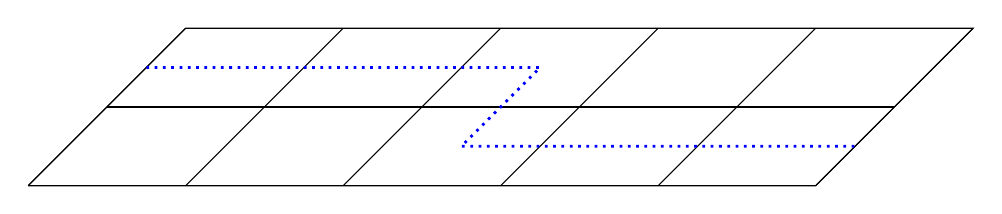
\begin{tikzpicture}[scale=2]
\def\rlvl{0.35}

% Grid
\draw (0,0) -- (1,1) -- (6,1) -- (5,0) -- (0,0);
\foreach \x in {0,1,...,5} {
    \draw (\x,0) -- (\x+1,1);
}
\draw (0.5,0.5) -- (5.5,0.5);

%Path
\draw[line width=0.35mm, blue, dotted] (0.75,0.75) -- (0.75+2.5,0.75) -- (0.75+2.5-0.5,0.75-0.5) -- (0.75+2.5-0.5+2.5,0.75-0.5);

% Raised squares
\raised{(1,0) rectangle (2,\rlvl)}{(2,0) -- (2.5,0.5) -- (2.5,0.5+\rlvl) -- (2,\rlvl)}{(2,\rlvl) -- (2.5,0.5+\rlvl) -- (1.5,0.5+\rlvl) -- (1,\rlvl)}
\raised{(1+2.5,0+0.5) rectangle (2+2.5,\rlvl+0.5)}{(2+2.5,0+0.5) -- (2.5+2.5,0.5+0.5) -- (2.5+2.5,0.5+\rlvl+0.5) -- (2+2.5,\rlvl+0.5)}{(2+2.5,\rlvl+0.5) -- (2.5+2.5,0.5+\rlvl+0.5) -- (1.5+2.5,0.5+\rlvl+0.5) -- (1+2.5,\rlvl+0.5)}
\raised{(1+2.5+1,0+0.5) rectangle (2+2.5+1,\rlvl+0.5)}{(2+2.5+1,0+0.5) -- (2.5+2.5+1,0.5+0.5) -- (2.5+2.5+1,0.5+\rlvl+0.5) -- (2+2.5+1,\rlvl+0.5)}{(2+2.5+1,\rlvl+0.5) -- (2.5+2.5+1,0.5+\rlvl+0.5) -- (1.5+2.5+1,0.5+\rlvl+0.5) -- (1+2.5+1,\rlvl+0.5)}
\end{tikzpicture}
}
    \caption{A grid of length $5$ with three raised squares and a path from left to right.}
    \label{fig:raised_grid}
\end{figure}

Let $G$ be the combinatorial class for passable grids. It is either the empty grid or contains at least one vertical slice. This is described by the admissible constructor disjoint union where a combinatorial class is split into nonintersecting parts. Now we have a combinatorial rule 
\[
    G \cong \set{\varepsilon} \sqcup G_{\geq 1}.
\]
In terms of generating functions this corresponds to addition, that is 
\[
    G(x) = 1 + G_{\geq1}(x).
\] 
Any valid grid consists of a combination of the vertical slices \gridN, \gridU\ and \gridD\ as one with both raised would block the path. We refer to a combinatorial object of length 1 as an \emph{atom}. The generating functions of the empty object and an atom are $1$ and $z$ respectively. Let $A$, $B$ and $C$ be the classes of passable grids starting with \gridN, \gridU\ and \gridD\ respectively and $D$ and $E$ the classes that can follow \gridU\ and \gridD\ respectively. Again we have a disjoint union 
\[
    G_{\geq1} \cong A \sqcup B \sqcup C.
\]
We define $\circ$ as the operator that prepends a vertical slice to all grids in a set. This is a Cartesian product, another admissible constructor denoted by $\times$, where
\[
X \times Y = \cset{(x,y)}{x\in X \text{ and } y \in Y}
\]
and in terms of generating functions corresponds to multiplication.

Now we have 
\[
    A \cong \gridN \circ G, \ B \cong \gridU \circ D \text{ and } C \cong \gridD \circ E.
\]
Following \gridU\ can be anything that does not start by blocking the lower square, that is 
\[
    D \cong \set{\varepsilon} \sqcup B \sqcup A
\]
and symmetrically we have 
\[
    E \cong \set{\varepsilon} \sqcup C \sqcup A.
\]
Now we have our specification, a system of rules with each class on the left at most once, defining an unambiguous formal grammar as shown in \FigureRef{fig:gridtree}.

\begin{figure}[ht!]
    \centering
    {
\newcommand{\gridnodeempty}{%
\begin{tikzpicture}[scale=0.3, baseline=(current bounding box.center)]
\useasboundingbox (0,-3) rectangle (3,3);
			\draw[thick, rounded corners=3pt] (0,0) rectangle (3,3);
			\draw[pattern=north west lines, pattern color=lightgray]  (3,0) to[rounded corners=3pt] (0,0) to[rounded corners=3pt] (0,3) to[rounded corners=3pt] (3,3) to[rounded corners=3pt] cycle;
;
			    \end{tikzpicture}
}

\newcommand{\gridnodesingle}[1]{%
\begin{tikzpicture}[scale=0.3, baseline=(current bounding box.center)]
\useasboundingbox (0,-3) rectangle (3,3);
			\draw[thick, rounded corners=3pt] (0,0) rectangle (3,3);
			\node at (1.5, 1.5) {#1};
;
			    \end{tikzpicture}
}


\begin{tikzpicture}[scale=0.8, every node/.style={scale=0.8}]
    \node (root) at (0, 0) {\gridnodesingle{$G$}};
    \node (lvl_1_1) at (-1.5, -2.25) {\gridnodeempty};
    \node (lvl_1_2) at (1.5, -2.25) {\gridnodesingle{$G_{\geq1}$}};
    \node (lvl_2_1) at (-3, -4.5) {\gridnodesingle{$A$}};
    \node (lvl_2_2) at (1.5, -4.5) {\gridnodesingle{$B$}};
    \node (lvl_2_3) at (6, -4.5) {\gridnodesingle{$C$}};
    \node (lvl_3_1) at (-4,-6.75) {\gridnodesingle{\gridN}};
    \node (lvl_3_2) at (-2,-6.75) {\gridnodesingle{$G$}};
    \node (lvl_3_3) at (0.5,-6.75) {\gridnodesingle{$D$}};
    \node (lvl_3_4) at (2.5,-6.75) {\gridnodesingle{\gridU}};
    \node (lvl_3_5) at (5,-6.75) {\gridnodesingle{\gridD}};
    \node (lvl_3_6) at (7,-6.75) {\gridnodesingle{$E$}};
    \node (lvl_4_1) at (-1,-9) {\gridnodeempty};
    \node (lvl_4_2) at (0.5,-9) {\gridnodesingle{$B$}};
    \node (lvl_4_3) at (2,-9) {\gridnodesingle{$A$}};
    \node (lvl_4_4) at (5.5,-9) {\gridnodeempty};
    \node (lvl_4_5) at (7,-9) {\gridnodesingle{$C$}};
    \node (lvl_4_6) at (8.5,-9) {\gridnodesingle{$A$}};
    
    \ptedge{(root)}{(-0.5,1.2)}{(lvl_1_1)}{(-0.5,1.3)}
    \ptedge{(root)}{(-0.5,1.2)}{(lvl_1_2)}{(-0.5,1.3)}
    
    \ptedge{(lvl_1_2)}{(-0.5,1.2)}{(lvl_2_1)}{(-0.5,1.3)}
    \ptedge{(lvl_1_2)}{(-0.5,1.2)}{(lvl_2_2)}{(-0.5,1.3)}
    \ptedge{(lvl_1_2)}{(-0.5,1.2)}{(lvl_2_3)}{(-0.5,1.3)}
    
    \ptedge{(lvl_2_1)}{(-0.5,1.2)}{(lvl_3_1)}{(-0.5,1.3)}
    \ptedge{(lvl_2_1)}{(-0.5,1.2)}{(lvl_3_2)}{(-0.5,1.3)}
    \ptedge{(lvl_2_2)}{(-0.5,1.2)}{(lvl_3_3)}{(-0.5,1.3)}
    \ptedge{(lvl_2_2)}{(-0.5,1.2)}{(lvl_3_4)}{(-0.5,1.3)}
    \ptedge{(lvl_2_3)}{(-0.5,1.2)}{(lvl_3_5)}{(-0.5,1.3)}
    \ptedge{(lvl_2_3)}{(-0.5,1.2)}{(lvl_3_6)}{(-0.5,1.3)}
    
    \ptedge{(lvl_3_3)}{(-0.5,1.2)}{(lvl_4_1)}{(-0.5,1.3)}
    \ptedge{(lvl_3_3)}{(-0.5,1.2)}{(lvl_4_2)}{(-0.5,1.3)}
    \ptedge{(lvl_3_3)}{(-0.5,1.2)}{(lvl_4_3)}{(-0.5,1.3)}
    \ptedge{(lvl_3_6)}{(-0.5,1.2)}{(lvl_4_4)}{(-0.5,1.3)}
    \ptedge{(lvl_3_6)}{(-0.5,1.2)}{(lvl_4_5)}{(-0.5,1.3)}
    \ptedge{(lvl_3_6)}{(-0.5,1.2)}{(lvl_4_6)}{(-0.5,1.3)}
\end{tikzpicture}
}
    \caption{The grammar for passable $2\times n$ grids.}
    \label{fig:gridtree}
\end{figure}

This system of rules when interpreted with generating functions is a set of equations with functions as its unknowns. In our example we have
\[
    \systeme*{G(z) = 1 + G_{\geq1}(z), G_{\geq1}(z) = A(z) + B(z) + C(z),A(z) = zG(z), B(z) = zD(z), C(z) = zE(z), D(z) = 1+B(z)+A(z), E(z) = 1+C(z)+A(z)}
\]
and solving for $G(z)$ gives 
\[
    G(z) = \frac{1+z}{1-2z-z^2}.
\]
The Taylor series for this function, at $z=0$, is
\[
    \sum_{i=0}^\infty \frac{G^{(i)}(0)}{i!}z^i = 1+3z+7z^2+17z^3+ 41z^4 + 99z^5 + \dotsm
\]
which corresponds to the number of grids for each size, e.g., there are 17 and 99 unique passable $2\times3$ and $2\times5$ grids respectively. We can even go further using calculus and find the exact formula, 
\[
|G_n| = \frac{\left(1+\sqrt{2}\right)^{n+1} + \left(1-\sqrt{2}\right)^{n+1}}{2}.
\]
This is not always the case and depends on the type of generating function we have.

In the context of this thesis, we will usually refer to combinatorial classes as just classes and the same goes for combinatorial specifications and rules. We also assume all constructors to be admissible and all rules to entail isomorphism. 

\section{Permutations\label{sec:permutations}}
A \emph{permutation} $\pi$ is a bijection between a set and itself. In our context, the set in question is $[n] = \setn$. We adopt a one line notation for permutations, $\pi = \perm{\pi}{n}$ where $\pi_i = j$ if $i$ maps to $j$. The permutation $1423$ maps $\{1,2,3,4\}$ to itself. This correspondence can be seen in \FigureRef{fig:perm_example} as well as a geometric representation of the permutation which displays the points $\cset{(i,\pi(i))}{i \in [n]}$ in the Cartesian plane.

\begin{figure}[ht!]
    \centering
    \begin{tikzpicture}[ele/.style={fill=black,circle,minimum width=.8pt,inner sep=1pt},every fit/.style={ellipse,draw,inner sep=15},scale=0.6, every node/.style={scale=0.6}]
    \draw[white] (0,0);
    \node[ele,label=left:$1$] (a1) at (0,4) {};    
    \node[ele,label=left:$2$] (a2) at (0,3) {};    
    \node[ele,label=left:$3$] (a3) at (0,2) {};
    \node[ele,label=left:$4$] (a4) at (0,1) {};
    
    \node[ele,,label=right:$1$] (b1) at (4,4) {};
    \node[ele,,label=right:$2$] (b2) at (4,3) {};
    \node[ele,,label=right:$3$] (b3) at (4,2) {};
    \node[ele,,label=right:$4$] (b4) at (4,1) {};
    
    \node[draw,fit= (a1) (a2) (a3) (a4),minimum width=2cm] {} ;
    \node[draw,fit= (b1) (b2) (b3) (b4),minimum width=2cm] {} ;  
    \draw[->,thick,shorten <=2pt,shorten >=2pt] (a1) -- (b1);
    \draw[->,thick,shorten <=2pt,shorten >=2] (a2) -- (b4);
    \draw[->,thick,shorten <=2pt,shorten >=2] (a3) -- (b2);
    \draw[->,thick,shorten <=2pt,shorten >=2] (a4) -- (b3);
\end{tikzpicture}
\hspace{2cm}
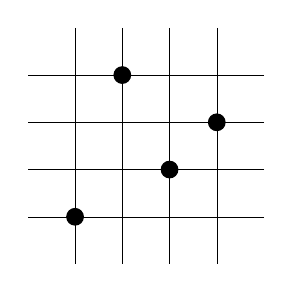
\begin{tikzpicture}[,scale=0.6, every node/.style={scale=0.6}]
        \foreach \x in {1,...,4} {
                \draw[ultra thin] (\x,5)--(\x,0);
                \draw[ultra thin] (5,\x)--(0,\x);
        }
        \draw[fill=black] (1,1) circle (5pt);
        \draw[fill=black] (2,4) circle (5pt);
        \draw[fill=black] (3,2) circle (5pt);
        \draw[fill=black] (4,3) circle (5pt);
\end{tikzpicture}

    \caption{The mapping and graphical representation of the permutation $1423$.}
    \label{fig:perm_example}
\end{figure}

A permutation on $[n]$ is said to be of length $n$ and $\mathcal{S}_n$ is the set of all permutations of length $n$. The set of permutations of length 3 is 
\[
    \mathcal{S}_3 = \{123,132,213,231,312,321\}.
\]
There is a permutation of length $0$, namely the empty permutation, denoted $\varepsilon$. This is the unique map from $\emptyset$ to $\emptyset$. The set of all permutations is denoted by $\mathcal{S}$. It is a combinatorial class since $\mathcal{S}_n$ is finite for all $n\in\N$, containing $n!$ elements.

Given a permutation $\pi = \perm{\pi}{n}$, its \emph{reverse} is
\[
    \rev(\pi) = \pi^\textsf{rev} = \wordrev{\pi}{n}
\]
and its \emph{inverse} is
\[
    \inv(\pi) = \pi^{-1} = \wordidx{\pi}{i}{n}
\]
where $\pi_{i_j} = k$ if $\pi_k = j$. The reverse of $132$ is $231$ and the inverse of $51324$ is $24351$. The reverse and inverse functions generate the dihedral group $D_4$, that is the symmetries of a square using the graphical representation of a permutation. We define these 8 symmetry maps as $\sym_1,\sym_2,\dotsc,\sym_8$ as is shown in \TableRef{tab:permsym} which also includes an example for the permutation $1423$.

\begin{table}[ht!]
    \centering
    {
\newcommand{\tsquare}[4]{\adjustbox{valign=t}{\begin{tikzpicture}\fill[white] (-.1,-.1) rectangle (.85,.85);\draw (0,0) rectangle (0.75,0.75); \draw (0,.75) node[xshift=1.4mm,yshift=-1.4mm] {\tiny{$#1$}}; \draw (.75,.75) node[xshift=-1.4mm,yshift=-1.4mm] {\tiny{$#2$}}; \draw (.75,.0) node[xshift=-1.4mm,yshift=1.4mm] {\tiny{$#3$}}; \draw (0,0) node[xshift=1.4mm,yshift=1.4mm] {\tiny{$#4$}};\end{tikzpicture}}}

\newcommand{\sA}{
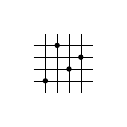
\begin{tikzpicture}[scale=0.15]
    \fill[white] (-.5,-.5) rectangle (5.5,5.5);
    \foreach \x in {1,...,4} {
        \draw[ultra thin] (\x,0)--(\x,5); %vline
        \draw[ultra thin] (0,\x)--(5,\x); %hline
    }
    \draw[fill=black] (1,1) circle (5pt);
    \draw[fill=black] (2,4) circle (5pt);
    \draw[fill=black] (3,2) circle (5pt);
    \draw[fill=black] (4,3) circle (5pt);
\end{tikzpicture}
}

\newcommand{\sB}{
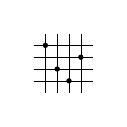
\begin{tikzpicture}[scale=0.15]
    \fill[white] (-.5,-.5) rectangle (5.5,5.5);
    \foreach \x in {1,...,4} {
        \draw[ultra thin] (\x,0)--(\x,5); %vline
        \draw[ultra thin] (0,\x)--(5,\x); %hline
    }
    \draw[fill=black] (1,4) circle (5pt);
    \draw[fill=black] (2,2) circle (5pt);
    \draw[fill=black] (3,1) circle (5pt);
    \draw[fill=black] (4,3) circle (5pt);
\end{tikzpicture}
}

\newcommand{\sC}{
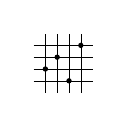
\begin{tikzpicture}[scale=0.15]
    \fill[white] (-.5,-.5) rectangle (5.5,5.5);
    \foreach \x in {1,...,4} {
        \draw[ultra thin] (\x,0)--(\x,5); %vline
        \draw[ultra thin] (0,\x)--(5,\x); %hline
    }
    \draw[fill=black] (1,2) circle (5pt);
    \draw[fill=black] (2,3) circle (5pt);
    \draw[fill=black] (3,1) circle (5pt);
    \draw[fill=black] (4,4) circle (5pt);
\end{tikzpicture}
}

\newcommand{\sD}{
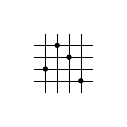
\begin{tikzpicture}[scale=0.15]
    \fill[white] (-.5,-.5) rectangle (5.5,5.5);
    \foreach \x in {1,...,4} {
        \draw[ultra thin] (\x,0)--(\x,5); %vline
        \draw[ultra thin] (0,\x)--(5,\x); %hline
    }
    \draw[fill=black] (1,2) circle (5pt);
    \draw[fill=black] (2,4) circle (5pt);
    \draw[fill=black] (3,3) circle (5pt);
    \draw[fill=black] (4,1) circle (5pt);
\end{tikzpicture}
}

\newcommand{\sE}{
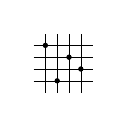
\begin{tikzpicture}[scale=0.15]
    \fill[white] (-.5,-.5) rectangle (5.5,5.5);
    \foreach \x in {1,...,4} {
        \draw[ultra thin] (\x,0)--(\x,5); %vline
        \draw[ultra thin] (0,\x)--(5,\x); %hline
    }
    \draw[fill=black] (1,4) circle (5pt);
    \draw[fill=black] (2,1) circle (5pt);
    \draw[fill=black] (3,3) circle (5pt);
    \draw[fill=black] (4,2) circle (5pt);
\end{tikzpicture}
}

\newcommand{\sF}{
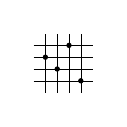
\begin{tikzpicture}[scale=0.15]
    \fill[white] (-.5,-.5) rectangle (5.5,5.5);
    \foreach \x in {1,...,4} {
        \draw[ultra thin] (\x,0)--(\x,5); %vline
        \draw[ultra thin] (0,\x)--(5,\x); %hline
    }
    \draw[fill=black] (1,3) circle (5pt);
    \draw[fill=black] (2,2) circle (5pt);
    \draw[fill=black] (3,4) circle (5pt);
    \draw[fill=black] (4,1) circle (5pt);
\end{tikzpicture}
}

\newcommand{\sG}{
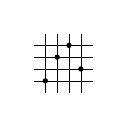
\begin{tikzpicture}[scale=0.15]
    \fill[white] (-.5,-.5) rectangle (5.5,5.5);
    \foreach \x in {1,...,4} {
        \draw[ultra thin] (\x,0)--(\x,5); %vline
        \draw[ultra thin] (0,\x)--(5,\x); %hline
    }
    \draw[fill=black] (1,1) circle (5pt);
    \draw[fill=black] (2,3) circle (5pt);
    \draw[fill=black] (3,4) circle (5pt);
    \draw[fill=black] (4,2) circle (5pt);
\end{tikzpicture}
}

\newcommand{\sH}{
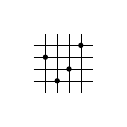
\begin{tikzpicture}[scale=0.15]
    \fill[white] (-.5,-.5) rectangle (5.5,5.5);
    \foreach \x in {1,...,4} {
        \draw[ultra thin] (\x,0)--(\x,5); %vline
        \draw[ultra thin] (0,\x)--(5,\x); %hline
    }
    \draw[fill=black] (1,3) circle (5pt);
    \draw[fill=black] (2,1) circle (5pt);
    \draw[fill=black] (3,2) circle (5pt);
    \draw[fill=black] (4,4) circle (5pt);
\end{tikzpicture}
}

\begin{tabular}{c|c|c|c|c|c}
    \adjustbox{valign=T}{$\textsf{sym}_0$} & \adjustbox{valign=T}{$\pi$} & \adjustbox{valign=T}{Rotate $0^\circ$} & \tsquare{A}{B}{C}{D} & \adjustbox{valign=T}{$1423$} & \adjustbox{valign=t}{\sA} \\
    \hline
    \adjustbox{valign=T}{$\textsf{sym}_1$} & \adjustbox{valign=T}{$\textsf{r}(\textsf{i}(\pi))$} & \adjustbox{valign=T}{Rotate $90^\circ$} & \tsquare{D}{A}{B}{C} & \adjustbox{valign=T}{$4213$} & \adjustbox{valign=t}{\sB}\\
    \hline
    \adjustbox{valign=T}{$\textsf{sym}_2$} & \adjustbox{valign=T}{$\textsf{i}(\textsf{r}(\textsf{i}(\textsf{r}(\pi))))$} & \adjustbox{valign=T}{Rotate $180^\circ$} & \tsquare{C}{D}{A}{B} & \adjustbox{valign=T}{$2314$} &\adjustbox{valign=t}{\sC} \\
    \hline
    \adjustbox{valign=T}{$\textsf{sym}_3$} & \adjustbox{valign=T}{$\textsf{i}(\textsf{r}(\pi))$} & \adjustbox{valign=T}{Rotate $270^\circ$} & \tsquare{B}{C}{D}{A} & \adjustbox{valign=T}{$2431$} & \adjustbox{valign=t}{\sD}\\
    \hline
    \adjustbox{valign=T}{$\textsf{sym}_4$} & \adjustbox{valign=T}{$\textsf{i}(\textsf{r}(\textsf{i}(\pi)))$} & \adjustbox{valign=T}{Horizontal flip} & \tsquare{D}{C}{B}{A} & \adjustbox{valign=T}{$4132$} &\adjustbox{valign=t}{\sE}\\
    \hline
    \adjustbox{valign=T}{$\textsf{sym}_5$} & \adjustbox{valign=T}{$\textsf{r}(\pi)$} & \adjustbox{valign=T}{Vertical flip} & \tsquare{B}{A}{D}{C} & \adjustbox{valign=T}{$3241$} &\adjustbox{valign=t}{\sF}\\
    \hline
    \adjustbox{valign=T}{$\textsf{sym}_6$} & \adjustbox{valign=T}{$\textsf{i}(\pi)$} & \adjustbox{valign=T}{Diagonal flip} & \tsquare{C}{B}{A}{D} & \adjustbox{valign=T}{$1342$} &\adjustbox{valign=t}{\sG}\\
    \hline
    \adjustbox{valign=T}{$\textsf{sym}_7$} & \adjustbox{valign=T}{$\textsf{r}(\textsf{i}(\textsf{r}(\pi)))$} & \adjustbox{valign=T}{Antidiagonal flip} & \tsquare{A}{D}{C}{B} & \adjustbox{valign=T}{$3124$} &\adjustbox{valign=t}{\sH}\\
\end{tabular}

}
    \caption{The 8 symmetry maps for permutations interpreted with reverse and inverse, dihedral group $D_4$ and an example for $\pi=1423$.}
    \label{tab:permsym}
\end{table}

We define $\sym(\pi) = \cset{\sym_i(\pi)}{i \in [8]}$ as the \emph{symmetries of} $\pi$. Note that two different symmetry functions can map to the same permutation, e.g., $\sym(1) = \set{1}$. Every permutation has between 1 and 8 symmetries.

Given a finite strictly totally ordered set $(M, <)$ where $M = \set{x_1,x_2,\dotsc,x_n}$, we define its \emph{sorting} as
\[
    \sort(M) = (x_{i_1},x_{i_2},\dotsc,x_{i_n})
\]
if $x_{i_1} < x_{i_2} < \dotsm < x_{i_n}$. Suppose $M=\set{1,5,2}$, then $\sort(M) = (1,2,5)$. The \emph{indexed subsequence} of a permutation $\pi \in \mathcal{S}_n$ for indices $S\subseteq [n]$ is the sequence
\[
    \sseq{S}{\pi}=\wordidx{\pi}{i}{|S|}
\]
if $\sort(S) = (i_1,i_2,\dotsc,i_{|S|})$. Given an indexed subsequence $\gamma$ of a permutation $\pi \in \mathcal{S}_n$, its \emph{standardization}, $\st{\gamma}$, is the sequence where the $i^\text{th}$ largest entry has been replaced by $i$. Let $\pi = 41253 \in \mathcal{S}_5$ and $S=\{1,3,4\}$, then $\st{\sseq{S}{\pi}} = \st{425} = 213$.

Given two permutations $\pi \in \mathcal{S}_n$ and $\sigma \in \mathcal{S}_k$ we say that $\pi$ \emph{contains} $\sigma$, denoted $\contains{\pi}{\sigma}$, if there exists a subset $S \subseteq [n]$ such that $\st{\sseq{S}{\pi}} = \sigma$. If $\pi$ does not contain $\sigma$, it \emph{avoids} it. In the context of containment, we usually refer to the contained permutation as a (classical) \emph{pattern}\footnote{There are other types of patterns that we do not concern ourselves with in this thesis.} and that permutations contain or avoid a pattern. The permutation $356214$ contains the pattern $4213$ since
\[
    \st{\sseq{\{2, 4, 5, 6\}}{356214}} = \st{5214} = 4213.
\]
It, however, avoids the pattern $1432$ since
\[
    1432 \notin \cset{\st{\sseq{S}{356214}}}{S \subseteq [6]}.
\]
An occurrence of $4213$ in $356214$ can be seen in \FigureRef{fig:pattern_containment}.

\begin{figure}[ht!]
    \centering
    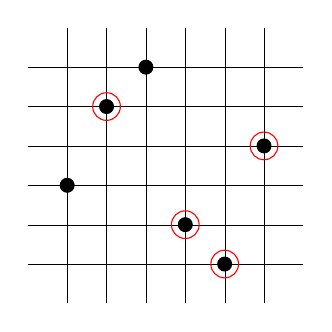
\begin{tikzpicture}[scale=.5,baseline=(current bounding box.center)]
    \foreach \x in {1,...,6} {
        \draw[ultra thin] (\x,0)--(\x,7); %vline
        \draw[ultra thin] (0,\x)--(7,\x); %hline
    }
    \draw[fill=black] (1,3) circle (5pt);
    \draw[fill=black] (2,5) circle (5pt);
    \draw[fill=black] (3,6) circle (5pt);
    \draw[fill=black] (4,2) circle (5pt);
    \draw[fill=black] (5,1) circle (5pt);
    \draw[fill=black] (6,4) circle (5pt);
    \draw[red] (2,5) circle (10pt);
    \draw[red] (4,2) circle (10pt);
    \draw[red] (5,1) circle (10pt);
    \draw[red] (6,4) circle (10pt);
\end{tikzpicture}
    \caption{The permutation $356214$ with an occurrence of $4213$ circled.}
    \label{fig:pattern_containment}
\end{figure}

A set of permutation $\Pi$ is \emph{closed downwards} with respect to containment if 
\[
    \bigcup_{\pi \in \Pi}\cset{\sigma \in \mathcal{S}}{\contains{\pi}{\sigma}} \subseteq \Pi.
\]
A set of permutations that is closed downwards is called a \emph{permutation class}. The set $\{\varepsilon, 1, 12, 123\}$ is closed downwards since all patterns contained in any of its elements belong to the set. We can extend this set to include all increasing permutations, $\set{\varepsilon, 1, 12, 123, 1234, \dotsc}$ and it is still closed downwards. Both sets are therefore permutation classes. Isorphism between permutation classes is often called \emph{Wilf equivalence} and their equivalence classes are called \emph{Wilf classes}. 

A permutation $\pi$ \emph{avoids} a set of permutations $\Pi$ if it avoids every $\sigma \in \Pi$. It \emph{contains} $\Pi$ if it does not avoid it, that is, it contains any permutation of $\Pi$. Let 
\[
    \Av{\Pi} = \cset{\pi \in \mathcal{S}}{\pi \text{ avoids } \Pi}.
\]
We may abuse this notation by omitting set brackets, writing $\Av{\sigma_1,\sigma_2}$ instead of $\Av{\set{\sigma_1,\sigma_2}}$. Define \[
    \Avn{n}{\Pi} = \cset{\pi \in \Av{\Pi}}{|\pi| = n}
\]
for $n\in\N$.

A set of permutations $\mathcal{B}$ is called a \emph{basis} if for all $\pi\in\mathcal{B}$ there does not exist a $\sigma \in \mathcal{B} \setminus \set{\pi}$ such that $\contains{\pi}{\sigma}$. The set $\{12,21\}$ is a basis while $\{12,231\}$ is not since $\contains{231}{12}$. Permutation classes can be described in terms of a basis avoided, e.g., 
\[
    \{\varepsilon,1,12,123\} = \Av{21, 1234}
\]
and
\[
    \{\varepsilon, 1, 12, 123, 1234,\dotsc\} = \Av{21}.
\]

Let $\mathcal{B}$ be a basis. We extent the definition of symmetry maps to bases such that
\[
    \sym_i(\mathcal{B}) = \cset{\sym_i(\sigma)}{\sigma \in \mathcal{B}}
\]
and
\[
    \sym(\mathcal{B}) = \cset{\sym_i(\mathcal{B})}{i \in [8]}.
\]
For any basis $\mathcal{B}$, the \emph{symmetry class} of $\Av{\mathcal{B}}$ is $\cset{\Av{B}}{B \in \sym(\mathcal{B})}$. The symmetry class of any permutation class is a subset of its Wilf class. As symmetries are considered trivial bijections we usually only concern ourselves with the lexicographically minimal representation of each symmetry class. For example, there are 7 symmetry classes and 3 Wilf classes for singleton bases in $\mathcal{S}_4$. They are shown in \TableRef{tab:wilfcls4}.

\begin{table}[ht!]
    \centering
    \begin{tabular}{c|c}
        Wilf class & Counting sequence\\
        \hline
        $\begin{matrix}\Av{1234}\\\Av{1243}\\\Av{1432}\\\Av{2143}\end{matrix}$ & $1, 2, 6, 23, 103, 513, 2761, 15767, \dotsc$ \\
        \hline
        $\begin{matrix}\Av{1324}\end{matrix}$ & $1, 2, 6, 23, 103, 513, 2762, 15793,\dotsc$\\
        \hline
        $\begin{matrix}\Av{1342}\\\Av{2413}\end{matrix}$ & $1, 2, 6, 23, 103, 512, 2740, 15485,\dotsc$
    \end{tabular}
    \caption{The $7$ lexicographical minimal representation of symmetry classes of permutation classes avoiding a single classical pattern of length $4$. They are grouped into $3$ Wilf classes by row.}
    \label{tab:wilfcls4}
\end{table}




\section{Gridded permutations\label{sec:griddedpermutations}}
A \emph{cell} $(a,b) \in \N^2$ is the region within $[0,\infty)^2$ defined by $[a, a+1) \times [b, b+1).$ A pair
\[
    (\pi,P) = (\perm{\pi}{n}, ((a_1,b_1),(a_2,b_2),\dotsc,(a_n,b_n)))
\]
where $P$ is a $n$-tuple of cells and $\pi$ is a permutation is called a \emph{gridded permutation} of length $n$ if for all $i,j \in [n]$, $i<j$ implies $a_i \leq a_j$ and $\pi_i < \pi_j$ implies $b_i \leq b_j$. A more detailed definition is given by Albert \cite{albert2012geometric}. We refer to $P$ as the \emph{positions} of the gridded permutation and $\pi$ as the \emph{underlying permutation}. We use a one line notation for gridded permutations 
\[
    \pi = \pi_1^{(a_1,b_1)}\pi_1^{(a_2,b_2)}\dotsb\pi_n^{(a_n,b_n)}
\]
where we can exclude all but the last position of consecutive occurrences of the same position. The gridded permutation $87^{(0,2)}1^{(1,0)}6^{(1,2)}2^{(1,0)}4^{(3,1)}3^{(3,0)}5^{(4,2)}$ can be seen in \FigureRef{fig:gridded_perm}.

\begin{figure}[ht!]
    \centering
    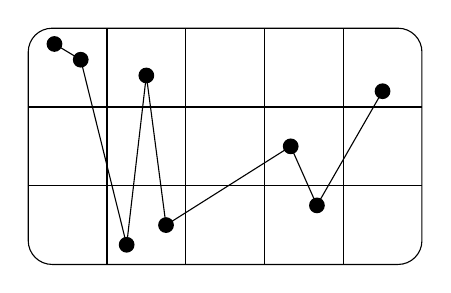
\begin{tikzpicture}
  \def\xs{1.0}
  \def\ys{1.0}
  \def\ps{1.0}
  \draw (0.001,0.001) grid[xscale=\xs,yscale=\ys] (4.999, 2.999);
  \draw[rounded corners=2ex] (0,0) rectangle (5,3);
  \coordinate (p0) at (0.3333333333333333*\xs,2.8*\ys);
  \coordinate (p1) at (0.6666666666666666*\xs,2.6*\ys);
  \coordinate (p2) at (1.25*\xs,0.25*\ys);
  \coordinate (p3) at (1.5*\xs,2.4*\ys);
  \coordinate (p4) at (1.75*\xs,0.5*\ys);
  \coordinate (p5) at (3.3333333333333335*\xs,1.5*\ys);
  \coordinate (p6) at (3.6666666666666665*\xs,0.75*\ys);
  \coordinate (p7) at (4.5*\xs,2.2*\ys);
  \draw (p0)--(p1)--(p2)--(p3)--(p4)--(p5)--(p6)--(p7);
  \fill (p0) circle (0.1*\ps);
  \fill (p1) circle (0.1*\ps);
  \fill (p2) circle (0.1*\ps);
  \fill (p3) circle (0.1*\ps);
  \fill (p4) circle (0.1*\ps);
  \fill (p5) circle (0.1*\ps);
  \fill (p6) circle (0.1*\ps);
  \fill (p7) circle (0.1*\ps);
\end{tikzpicture}
    \caption{The gridded permutation $87^{(0,2)}1^{(1,0)}6^{(1,2)}2^{(1,0)}4^{(3,1)}3^{(3,0)}5^{(4,2)}$.}
    \label{fig:gridded_perm}
\end{figure}

We extend the definition of indexed subsequences to gridded permutations so the sequence produced, $\sseq{S}{\pi}$, contains elements of the underlying permutation and positions. Given this extension, we can also extend the standardization of an indexed subsequence of a gridded permutation to be applied only to the underlying permutation. For example, given a gridded permutation $\pi = 1^{(0,0)}5^{(1,2)}2^{(2,0)}43^{(2,1)}$ and $S=\set{1,2,5}$ we have
\[
\st{\sseq{S}{\pi}} = \st{1^{(0,0)}5^{(1,2)}3^{(2,1)}} = 1^{(0,0)}3^{(1,2)}2^{(2,1)}.
\]
Using the extended definition of standardization we extend containment and avoidance to gridded permutations, for both single and sets of gridded permutations. For example, the gridded permutation $1^{(0,0)}5^{(1,2)}2^{(2,0)}43^{(2,1)}$ contains $1^{(0,0)}2^{(2,0)}3^{(2,1)}$ but avoids $1^{(0,0)}23^{(2,1)}$.

Let $\mathcal{G}$ be the set of all gridded permutations and $\mathcal{G}_n$ its subset with only gridded permutations of length $n$. The set $\mathcal{G}$ is not a combinatorial class since $\mathcal{G}_n$ is infinite for all $n \in \Z^+$, having infinitely many cells to choose from. If we restrict the choice of cells to be finite, then so are the gridded permutations we can form. Let $\mathcal{G}^{(c,r)}$ be the set of gridded permutation with positions in 
\[
\{0,1,\dotsc,c-1\} \times \{0,1,\dotsc,r-1\}
\]
and
\[
\mathcal{G}^{(c,r)}_n = \cset{\pi \in \mathcal{G}^{(c,r)}}{|\pi| = n}.
\]
The set $\mathcal{G}^{(c,r)}$ is a combinatorial class. Define
\[
    \textsf{Av}^{(c,r)}\left(\Pi\right) = \cset{\pi \in \mathcal{G}^{(c,r)}}{\pi \text{ avoids } \Pi}
\]
and
\[
    \textsf{Av}_n^{(c,r)}\left(\Pi\right) = \cset{\pi \in \mathcal{G}_n^{(c,r)}}{\pi \text{ avoids } \Pi}.
\]

\section{Tilings\label{sec:tilings}}
A \emph{tiling} is a triple
\[
\mathcal{T} = ((c,r), \mathcal{O}, \set{\mathcal{R}_1,\mathcal{R}_2,\dotsc,\mathcal{R}_k})
\]
where
\[
    (c,r) \in \Z^+ \times \Z^+, \ \mathcal{O} \subseteq \mathcal{G}^{(c,r)} \text{ and } \mathcal{R}=\set{\mathcal{R}_1,\mathcal{R}_2,\dotsc,\mathcal{R}_k} \subseteq \left(\mathcal{G}^{(c,r)}\right)^k
\]
are called \emph{dimension}, \emph{obstructions} and \emph{requirements} respectively. The gridded permutations in $\textsf{Av}^{(c,r)}\left(\mathcal{O}\right)$ that contain $\mathcal{R}_1,\dotsc,\mathcal{R}_k$ make up the combinatorial class $\textsf{Grid}(\mathcal{T})$. A more detailed definition is given by Bean \cite{BeanPhd:phd}. An example of a tiling can be seen in \FigureRef{fig:tiling_example} where obstructions are red and requirements blue. Positions with $12$ and $21$ obstruction and a $1$ requirement are represented with a larger black point.

\begin{figure}[ht!]
    \centering
    {
% rect
%\newcommand{\reqpnt}[3]{\fill[blue] (#1-#3,#2-#3) rectangle (#1+#3,#2+#3);}
% donut
%\newcommand{\reqpnt}[3]{\fill[blue] (#1,#2) circle (#3); \fill[white] (#1,#2) circle (#3 * 0.5);}
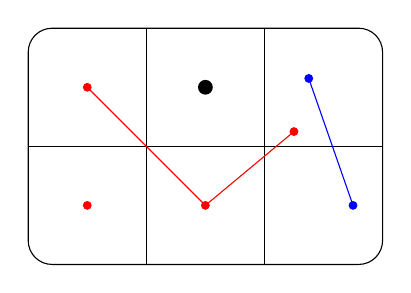
\begin{tikzpicture}[scale=0.75, every node/.style={scale=0.75}]
    \def\spnt{0.075} % Size of smaller points
    \def\lpnt{0.125} % Size of larger points
    \draw[rounded corners=2ex] (0,0) rectangle (6,4);
    \draw (2.0, 4) -- (2.0, 0);
    \draw (4.0, 4) -- (4.0, 0);
    \draw (0, 2) -- (6.0, 2);
    \fill[red] (1, 3) circle (\spnt);
    \fill[red] (1, 1) circle (\spnt);
    \fill[red] (3, 1) circle (\spnt);
    \fill[red] (4.5, 2.25) circle (\spnt);
    \draw[red] (1, 3) -- (3,1) -- (4.5,2.25);
    \fill (3,3) circle (\lpnt);
    \draw[blue] (4.75, 3.15) -- (5.5,1);
    \fill[blue] (4.75, 3.15) circle (\spnt);
    \fill[blue] (5.5, 1) circle (\spnt);
    %\reqpnt{4.75}{3.15}{\spnt*1.2}
    %\reqpnt{5.5}{1}{\spnt*1.2}
\end{tikzpicture}
}
    \caption{A $3 \times 2$ tiling with $\mathcal{R} = \set{\set{1^{(1,1)}}, \set{2^{(1,1)}1^{(2,0)}}}$ and $\mathcal{O}$ consisting of $1^{(0,0)}$, $12^{(1,1)}$, $21^{(1,1)}$ and $3^{(0,1)}1^{(1,0)}2^{(2,1)}$.}
    \label{fig:tiling_example}
\end{figure}

Typically, when we want to enumerate $\Av{132}$ we start with a disjoint union constructor as it is either empty or contains a largest point. If it contains a largest point, it must still avoid 132 on either side. Furthermore, the elements to the left of the largest point must be greater than those to its right or you have an occurrence of $132$ with the largest point. This is important since it allows us to uniquely map the elements to the right of the largest point from the rule. Now we have a specification
\begin{align*}
\Av{132} &\cong \set{\varepsilon} \sqcup \textsf{Av}_{\geq1}(132)\\
\textsf{Av}_{\geq1}(132) &\cong \Av{132} \times \set{\point{0.1}} \times \Av{132}
\end{align*}
and a generating function
\[
\frac{1-\sqrt{1-4z}}{2z}.
\]
This is a simple example but given different classes and constructors, we can end up with classes that are difficult to describe accurately. The purpose of tilings is to provide a sort of language to describe classes with more complicated permutation constraints or limited parts of permutations, e.g., we can describe $\textsf{Av}_{\geq1}(132)$ with the tiling seen in \FigureRef{fig:tiling132}.

\begin{figure}[ht!]
    \centering
    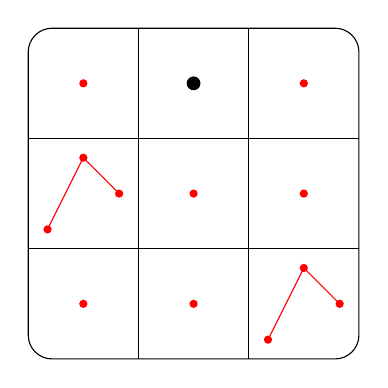
\begin{tikzpicture}[scale=0.7, every node/.style={scale=0.7}]
    \def\spnt{0.075} % Size of smaller points
    \def\lpnt{0.125} % Size of larger points
    \draw[rounded corners=2ex] (0,0) rectangle (6,6);
    \draw (2.0, 6) -- (2.0, 0);
    \draw (4.0, 6) -- (4.0, 0);
    \draw (0, 2) -- (6.0, 2);
    \draw (0, 4) -- (6.0, 4);
    \fill[red] (1, 5) circle (\spnt);
    \fill[red] (1, 1) circle (\spnt);
    \fill[red] (3, 3) circle (\spnt);
    \fill[red] (3, 1) circle (\spnt);
    \fill[red] (5, 5) circle (\spnt);
    \fill[red] (5, 3) circle (\spnt);
    \fill (3,5) circle (\lpnt);
    \draw[red] (0.25+0.1, 2.25+0.1) -- (1,3.75-0.1) -- (1.75-0.1,3);
    \draw[red] (4.25+0.1, 0.25+0.1) -- (5,1.75-0.1) -- (5.75-0.1,1);
    \fill[red] (0.25+0.1, 2.25+0.1) circle (\spnt);
    \fill[red] (1,3.75-0.1) circle (\spnt);
    \fill[red] (1.75-0.1,3) circle (\spnt);
    \fill[red] (4.25+0.1, 0.25+0.1) circle (\spnt);
    \fill[red] (5,1.75-0.1) circle (\spnt);
    \fill[red] (5.75-0.1,1) circle (\spnt);
\end{tikzpicture}
    \caption{A tiling $\mathcal{T}$ with $\textsf{Grid}(\mathcal{T})$ isomorphic to $\textsf{Av}_{\geq1}(132)$.}
    \label{fig:tiling132}
\end{figure}

\section{Combinatorial Exploration}
Combinatorial Exploration \cite{css} is a domain agnostic specification searcher. It uses strategies to generate rules for classes. Strategies are independent of classes and describe an action that may result in rules given an applicable class. 

The search method is done in a breadth-first manner from the root class. It uses a predefined set of strategies to generate rules for classes and expands a universe in the hope that it contains a specification.

To avoid tautologies, the searcher gives classes equivalence labels and tracks rules in terms of parent and children pairs in term of their equivalence labels. The rules within a single equivalence label may or may not be equivalence rules. Any single child rule that could result in a tautology could be contained in an equivalence label with nonequivalent classes. When the specification is found and extracted from the universe, any sequence of equivalence rules is merged into a single rule.

\section{TileScope}
TileScope \cite{tiling} is an implementation of Combinatorial Exploration for tilings. The root class usually has a single cell and no requirements and therefore a direct correspondence to a permutation class. The library also utilizes Permuta \cite{permuta}, a general permutation library. Most of the strategies TileScope uses can be found in Bean \cite{BeanPhd:phd}. We will explain those that are not.

\subsection{Column reverse}
\begin{definition}\label{def:rrgp}
Let $\pi=\pi_1^{(x_1,y_1)}\pi_2^{(x_2,y_2)}\dotsm\pi_n^{(x_n,y_n)} \in \mathcal{G}_n$ and define its \emph{column reverse} for $(a,b)\in\N^2$ where $a\leq b$ as the mapping $\textsf{rev}_{[a,b]}$ that reverses the longest subsequence of $\pi$ who's columns all belong to $[a,b]$.
\end{definition}

The column reverse can be extended to tilings such that it is applied to all of its obstructions and requirements. Let $\pi = 5^{(0,1)}2^{(0,0)}4^{(1,1)}1^{(1,0)}6^{(2,2)}3^{(3,1)}$, then $\textsf{rev}_{[1,2]}(\pi) = 5^{(0,1)}2^{(0,0)}6^{(1,2)}1^{(2,0)}4^{(2,1)}3^{(3,1)}$, as shown in \FigureRef{fig:gp_col_rev}. An example for tilings can be seen in \FigureRef{fig:t_col_rev}.

\begin{figure}[ht!]
    \centering
    {
\newcommand{\picw}{1}
\newcommand{\pich}{1}
\begin{tikzpicture}
    \fill[gray!20] (\picw,0) rectangle (3*\picw,3*\pich);
    \draw (1 * \picw, 0) -- (1 * \picw, \pich * 3);
    \draw (2 * \picw, 0) -- (2 * \picw, \pich * 3);
    \draw (3 * \picw, 0) -- (3 * \picw, \pich * 3);
    \draw (0, 1 * \pich) -- (4 * \picw, 1 * \pich);
    \draw (0, 2 * \pich) -- (4 * \picw, 2 * \pich);
    \draw[rounded corners=2ex] (0,0) rectangle (4*\picw,3*\pich);
    \draw (0.25*\picw,3.5*0.5*\pich) -- (0.75*\picw,1*0.5*\pich) -- (1.25*\picw,3*0.5*\pich) -- (1.75*\picw,0.5*0.5*\pich) -- (2.5*\picw,5*0.5*\pich) -- (3.5*\picw,2.5*0.5*\pich);
    \fill (0.25*\picw,3.5*0.5*\pich) circle (0.075) node[below] {$5$};
    \fill (0.75*\picw,1*0.5*\pich) circle (0.075) node[below] {$2$};
    \fill (1.25*\picw,3*0.5*\pich) circle (0.075) node[above] {$4$};
    \fill (1.75*\picw,0.5*0.5*\pich) circle (0.075) node[left] {$1$};
    \fill (2.5*\picw,5*0.5*\pich) circle (0.075) node[above] {$6$};
    \fill (3.5*\picw,2.5*0.5*\pich) circle (0.075) node[above] {$3$};
\end{tikzpicture}
\begin{tikzpicture}
    \draw[white] (0,0) rectangle (2,3*\pich);
    \draw[thick, ->] (0.25,1.5*\pich) -- (1.75,1.5*\pich) node[above,pos=.5] {$\textsf{rev}_{[1,2]}$};
\end{tikzpicture}
\begin{tikzpicture}
    \fill[gray!20] (\picw,0) rectangle (3*\picw,3*\pich);
    \draw (1 * \picw, 0) -- (1 * \picw, \pich * 3);
    \draw (2 * \picw, 0) -- (2 * \picw, \pich * 3);
    \draw (3 * \picw, 0) -- (3 * \picw, \pich * 3);
    \draw (0, 1 * \pich) -- (4 * \picw, 1 * \pich);
    \draw (0, 2 * \pich) -- (4 * \picw, 2 * \pich);
    \draw[rounded corners=2ex] (0,0) rectangle (4*\picw,3*\pich);
    \draw (0.25*\picw,3.5*0.5*\pich) -- (0.75*\picw,1*0.5*\pich) -- (1.5*\picw,5*0.5*\pich) -- (2.25*\picw,0.5*0.5*\pich) -- (2.75*\picw,3*0.5*\pich) -- (3.5*\picw,2.5*0.5*\pich);
    \fill (0.25*\picw,3.5*0.5*\pich) circle (0.075) node[below] {$5$};
    \fill (0.75*\picw,1*0.5*\pich) circle (0.075) node[below] {$2$};
    \fill (1.5*\picw,5*0.5*\pich) circle (0.075) node[above] {$6$};
    \fill (2.25*\picw,0.5*0.5*\pich) circle (0.075) node[right] {$1$};
    \fill (2.75*\picw,3*0.5*\pich) circle (0.075) node[above] {$4$};
    \fill (3.5*\picw,2.5*0.5*\pich) circle (0.075) node[above] {$3$};
\end{tikzpicture}
}
    \caption{The column reverse of a gridded permutation.}
    \label{fig:gp_col_rev}
\end{figure}

\begin{figure}[ht!]
    \centering
    
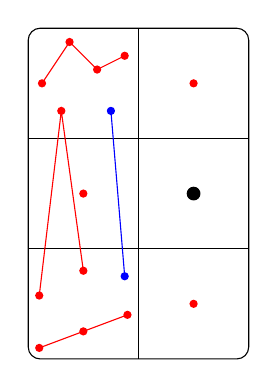
\begin{tikzpicture}[scale=0.7, every node/.style={scale=0.7}]
	\fill (3,3) circle (0.125);
	\fill[red] (1,3) circle (0.075);
	\fill[red] (3,5) circle (0.075);
	\fill[red] (3,1) circle (0.075);
    \draw[rounded corners=1ex] (0,0) rectangle (4,6);
    \draw (0,2) -- (4,2);
    \draw (0,4) -- (4,4);
    \draw (2,0) -- (2,6);
	\coordinate (a1) at (0.2,0.2);
	\coordinate (a2) at (1,0.5);
	\coordinate (a3) at (1.8,0.8);
	\coordinate (b1) at (0.2,1.15);
	\coordinate (b2) at (0.6,4.5);
	\coordinate (b3) at (1,1.6);
	\coordinate (c1) at (0.25,5);
	\coordinate (c2) at (0.75,5.75);
	\coordinate (c3) at (1.25,5.25);
	\coordinate (c4) at (1.75,5.5);
	\coordinate (d1) at (1.5,4.5);
	\coordinate (d2) at (1.75,1.5);
	\fill[red] (a1) circle (0.075);
	\fill[red] (a2) circle (0.075);
	\fill[red] (a3) circle (0.075);
	\fill[red] (b1) circle (0.075);
	\fill[red] (b2) circle (0.075);
	\fill[red] (b3) circle (0.075);
	\fill[red] (c1) circle (0.075);
	\fill[red] (c2) circle (0.075);
	\fill[red] (c3) circle (0.075);
	\fill[red] (c4) circle (0.075);
	\fill[blue] (d1) circle (0.075);
	\fill[blue] (d2) circle (0.075);
	\draw[red] (a1) -- (a2) -- (a3);
	\draw[red] (b1) -- (b2) -- (b3);
	\draw[red] (c1) -- (c2) -- (c3) -- (c4);
	\draw[blue] (d1) -- (d2);
\end{tikzpicture}
\begin{tikzpicture}[scale=0.7]
	\draw[white] (0,0) rectangle (2,6);
	\draw[thick, ->] (-.5,3) -- (2.5,3) node[above,pos=.5] {$\textsf{rev}_{[0,0]}$};
\end{tikzpicture}
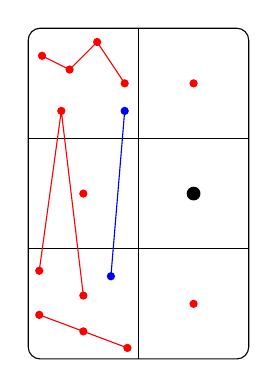
\begin{tikzpicture}[scale=0.7, every node/.style={scale=0.7}]
	\fill (3,3) circle (0.125);
	\fill[red] (1,3) circle (0.075);
	\fill[red] (3,5) circle (0.075);
	\fill[red] (3,1) circle (0.075);
    \draw[rounded corners=1ex] (0,0) rectangle (4,6);
    \draw (0,2) -- (4,2);
    \draw (0,4) -- (4,4);
    \draw (2,0) -- (2,6);
	\coordinate (a1) at (1.8,0.2);
	\coordinate (a2) at (1,0.5);
	\coordinate (a3) at (0.2,0.8);
	\coordinate (b1) at (1,1.15);
	\coordinate (b2) at (0.6,4.5);
	\coordinate (b3) at (0.2,1.6);
	\coordinate (c1) at (1.75,5);
	\coordinate (c2) at (1.25,5.75);
	\coordinate (c3) at (0.75,5.25);
	\coordinate (c4) at (0.25,5.5);
	\coordinate (d1) at (1.75,4.5);
	\coordinate (d2) at (1.5,1.5);
	\fill[red] (a1) circle (0.075);
	\fill[red] (a2) circle (0.075);
	\fill[red] (a3) circle (0.075);
	\fill[red] (b1) circle (0.075);
	\fill[red] (b2) circle (0.075);
	\fill[red] (b3) circle (0.075);
	\fill[red] (c1) circle (0.075);
	\fill[red] (c2) circle (0.075);
	\fill[red] (c3) circle (0.075);
	\fill[red] (c4) circle (0.075);
	\fill[blue] (d1) circle (0.075);
	\fill[blue] (d2) circle (0.075);
	\draw[red] (a1) -- (a2) -- (a3);
	\draw[red] (b1) -- (b2) -- (b3);
	\draw[red] (c1) -- (c2) -- (c3) -- (c4);
	\draw[blue] (d1) -- (d2);
\end{tikzpicture}
    \caption{The column reverse of a tiling.}
    \label{fig:t_col_rev}
\end{figure}

\begin{lemma}\label{lem:crevcontain}
Let $\pi, \sigma \in \mathcal{G}$ such that $\contains{\pi}{\sigma}$, then $\contains{\textsf{rev}_{[a,b]}(\pi)}{\textsf{rev}_{[a,b]}(\sigma)}$.
\end{lemma}
\begin{proof}
If $\pi$ has no elements within the columns then neither does $\sigma$ and both are mapped to themselves. If $\sigma$ has no elements within the columns then the mapping has no effect on the pattern which remains in $\textsf{rev}_{[a,b]}(\pi)$. 

Let $\set{i,i+1,\dotsc,i+k}$ be the indices of elements of $\pi$ within the columns. Let $\sigma = \st{\sseq{A_1\cup L \cup A_2}{\pi}}$ where $L \subseteq \set{i,i+1,\dotsc,i+k}$ and $A_1$ and $A_2$ are the indices in $\pi$ on either side of the columns.

\begin{align*}
    \textsf{rev}_{[a,b]}(\sigma) &= \st{\sseq{A_1}{\pi}\rev\left(\sseq{L}{\pi}\right)\sseq{A_2}{\pi}} \\
    &= \st{\sseq{A_1}{\textsf{rev}_{[a,b]}(\pi)}\sseq{\cset{2i+k-\ell}{\ell \in L}}{\textsf{rev}_{[a,b]}(\pi)}\sseq{A_2}{\textsf{rev}_{[a,b]}(\pi)}}\\
    &= \st{\sseq{A_1 \cup \cset{2i+k-\ell}{\ell \in L} \cup A_2}{\textsf{rev}_{[a,b]}(\pi)}}
\end{align*}
\end{proof}

\begin{lemma}\label{lem:crevgrid}
Let $\mathcal{T}$ be a tiling and $\pi \in \textsf{Grid}(\mathcal{T})$, then $\textsf{rev}_{[a,b]}(\pi)\in\textsf{Grid}(\textsf{rev}_{[a,b]}(\mathcal{T}))$.
\end{lemma}
\begin{proof}
By Lemma \ref{lem:crevcontain} all occurrences of requirements are preserved so the only way that $\textsf{rev}_{[a,b]}(\pi)$ is not in $\textsf{Grid}(\textsf{rev}_{[a,b]}(\mathcal{T}))$ is if there exists an obstruction $o$ that is avoided by $\pi$ while $\textsf{rev}_{[a,b]}(\pi)$ contains $\textsf{rev}_{[a,b]}(o)$. Suppose that there is such an obstruction, then $\textsf{rev}_{[a,b]}(\textsf{rev}_{[a,b]}(\pi)) = \pi$ must contain $\textsf{rev}_{[a,b]}(\textsf{rev}_{[a,b]}(o)) = o$ which contradicts $\pi$ avoiding $o$.
\end{proof}

\begin{proposition}\label{prop:rrtil}
Let $\mathcal{T}$ be a tiling, then $|\textsf{Grid}_n(\mathcal{T})| = |\textsf{Grid}_n(\textsf{rev}_{[a,b]}(\mathcal{T}))|$ for all $n\in\N$.
\end{proposition}
\begin{proof}
For any $\pi \in \textsf{Grid}_n(\mathcal{T})$ we have $(\textsf{rev}_{[a,b]} \circ \textsf{rev}_{[a,b]})(\pi) = \pi$ and therefore $\textsf{rev}_{[a,b]}$ is a bijection between $\textsf{Grid}_n(\mathcal{T})$ and $\cset{\textsf{rev}_{[a,b]}(\pi)}{\pi \in \textsf{Grid}_n(\mathcal{T})}$ with the latter being a subset of $\textsf{Grid}_n(\textsf{rev}_{[a,b]}(\mathcal{T}))$ by Lemma \ref{lem:crevgrid} and therefore $|\textsf{Grid}_n(\mathcal{T})| \leq |\textsf{Grid}_n(\textsf{rev}_{[a,b]}(\mathcal{T}))|$. By the same argument there is a bijection between $\textsf{Grid}_n(\textsf{rev}_{[a,b]}(\mathcal{T}))$ and
\[
    \cset{\textsf{rev}_{[a,b]}(\pi)}{\pi \in \textsf{Grid}_n(\textsf{rev}_{[a,b]}(\mathcal{T}))}
\]
with the latter being a subset of $\textsf{Grid}_n(\textsf{rev}_{[a,b]}(\textsf{rev}_{[a,b]}(\mathcal{T})))=\textsf{Grid}_n(\mathcal{T})$ and therefore $|\textsf{Grid}_b(\mathcal{T})| \geq |\textsf{Grid}(\textsf{rev}_{[a,b]}(\mathcal{T}))|$ and thus $|\textsf{Grid}_n(\mathcal{T})| = |\textsf{Grid}(\textsf{rev}_{[a,b]}(\mathcal{T}))|$
\end{proof}
\subsection{Column permutation}
Let $\pi=\pi_1^{(x_1,y_1)}\pi_2^{(x_2,y_2)}\dotsm\pi_n^{(x_n,y_n)} \in \mathcal{G}_n$ and define $\chi_x(\pi) = \pi_1^{(x,y_1)}\pi_2^{(x,y_2)}\dotsm\pi_n^{(x,y_n)}$, e.g.,
\[
\chi_{1}\left(1^{(0,0)}3^{(2,3)}2^{(5,2)}\right) = 1^{(1,0)}3^{(1,3)}2^{(1,2)}.
\]
This can also be extended to subsequences of gridded permutations.

\begin{definition}
Let $\pi = \pi_1^{(x_1,y_1)}\pi_2^{(x_2,y_2)}\dotsm\pi_n^{(x_n,y_n)} \in \mathcal{G}_n^{(c,r)}$ and $\sigma \in \mathcal{S}_k$ for $k \geq c$. The \emph{column permutation} $\sigma$ of $\pi$ is 
\[
    C_\sigma(\pi) = \chi_0(\sseq{A_{\sigma_1}}{\pi})\chi_1(\sseq{A_{\sigma_2}}{\pi}) \dotsm \chi_{k-1}(\sseq{A_{\sigma_k}}{\pi})
\]
where $A_i = \cset{j \in [n]}{x_j = i - 1}$ for $i \in [k]$.
\end{definition}

Note that $A_1,A_2,\dotsc,A_k$ can include empty sets and $\sigma$ can be larger than the number of columns the gridded permutation spans, but not vice versa. We extend this definition to tilings such that it is applied to all of its obstructions and requirements. Let $\sigma = 4312$ and
\[
\pi = 6^{(0,1)}2^{(0,0)}5^{(1,1)}3^{(1,0)}8^{(1,2)}4^{(2,1)}7^{(3,2)}1^{(3,0)},
\]
then $A_1=\set{1,2}$, $A_2=\set{3,4,5}$, $A_3=\set{6}$, $A_4=\set{7,8}$ and we have
\begin{align*}
    C_\sigma(\pi) &= \chi_0\left(\sseq{A_{\sigma_1}}{\pi}\right)\chi_1\left(\sseq{A_{\sigma_2}}{\pi}\right)\chi_2\left(\sseq{A_{\sigma_3}}{\pi}\right) \chi_3\left(\sseq{A_{\sigma_{4}}}{\pi}\right) \\
    &= \chi_0\left(\sseq{A_{4}}{\pi}\right)\chi_1\left(\sseq{A_{3}}{\pi}\right)\chi_2\left(\sseq{A_{1}}{\pi}\right)\chi_3\left(\sseq{A_{2}}{\pi}\right) \\
    &= \chi_0\left(\sseq{{\set{7,8}}}{\pi}\right) \chi_1\left(\sseq{{\set{6}}}{\pi}\right)\chi_2\left(\sseq{{\set{1,2}}}{\pi}\right)\chi_3\left(\sseq{\set{3,4,5}}{\pi}\right) \\
    &= \chi_0\left(7^{(3,2)}1^{(3,0)}\right)\chi_1\left(4^{(2,1)}\right)\chi_2\left(6^{(0,1)}2^{(0,0)}\right)\chi_3\left(5^{(1,1)}3^{(1,0)}8^{(1,2)}\right) \\
    &= 7^{(0,2)}1^{(0,0)}4^{(1,1)}6^{(2,1)}2^{(2,0)}5^{(3,1)}3^{(3,0)}8^{(3,2)}
\end{align*}
as is shown in \FigureRef{fig:gp_col_perm}. An example for tilings can be seen in \FigureRef{fig:t_col_perm}.

\begin{figure}[ht!]
    \centering
    {
\newcommand{\myscale}{0.7}
\begin{tikzpicture}[scale=\myscale, every node/.style={scale=\myscale}]
    \draw[rounded corners=2ex] (0,0) rectangle (8,6);
    \foreach \x in {2,4,6} {
        \draw (\x,0) -- (\x,6);
    }
    \foreach \y in {2,4} {
        \draw (0,\y) -- (8, \y);
    }
    \draw (0.5,3.5) -- (1.5,1) -- (2.5,3) -- (3,1.5) -- (3.5,5.5) -- (5,2.5) -- (6.5,4.5) -- (7.5,.5);
    
    \fill (0.5,3.5) circle (0.1) node[above] {$6$};
    \fill (1.5,1) circle (0.1) node[below] {$2$};
    \fill (2.5,3) circle (0.1) node[above] {$5$};
    \fill (3,1.5) circle (0.1) node[below] {$3$};
    \fill (3.5,5.5) circle (0.1) node[above] {$8$};
    \fill (5,2.5) circle (0.1) node[below] {$4$};
    \fill (6.5,4.5) circle (0.1) node[above] {$7$};
    \fill (7.5,.5) circle (0.1) node[below] {$1$};
    \foreach \x in {1,2,3,4} {
        \draw (\x*2-1, 0) node[below] {$\x$};
    }
\end{tikzpicture}
\begin{tikzpicture}[scale=\myscale]
    \draw[white] (0,0) rectangle (2,6);
    \draw[thick, ->] (0,3.4) -- (2,3.4) node[above,pos=.5] {$C_{4312}$};
\end{tikzpicture}
\begin{tikzpicture}[scale=\myscale, every node/.style={scale=\myscale}]
    \draw[rounded corners=2ex] (0,0) rectangle (8,6);
    \foreach \x in {2,4,6} {
        \draw (\x,0) -- (\x,6);
    }
    \foreach \y in {2,4} {
        \draw (0,\y) -- (8, \y);
    }
    \draw (0.5,4.5) -- (1.5,.5) -- (3,2.5) -- (4.5,3.5) -- (5.5,1) -- (6.5,3) -- (7,1.5) -- (7.5,5.5);
    \fill (0.5,4.5) circle (0.1) node[above] {$7$};
    \fill (1.5,.5) circle (0.1) node[below] {$1$};
    \fill (3,2.5) circle (0.1) node[below] {$4$};
    \fill (4.5,3.5) circle (0.1) node[above] {$6$};
    \fill (5.5,1) circle (0.1) node[below] {$2$};
    \fill (6.5,3) circle (0.1) node[above] {$5$};
    \fill (7,1.5) circle (0.1) node[below] {$3$};
    \fill (7.5,5.5) circle (0.1) node[above] {$8$};
    \draw (1,0) node[below] {$4$};
    \draw (3,0) node[below] {$3$};
    \draw (5,0) node[below] {$1$};
    \draw (7,0) node[below] {$2$};
\end{tikzpicture}
}
    \caption{The column permutation of a gridded permutation.}
    \label{fig:gp_col_perm}
\end{figure}

\begin{figure}[ht!]
    \centering
    {
\newcommand{\myscale}{0.75}
\begin{tikzpicture}[scale=\myscale, every node/.style={scale=\myscale}]
    \def\xscale{1.0} % Horizontal scale factor
    \def\yscale{0.95} % Vertical scale factor
    \def\spnt{0.075} % Size of smaller points
    \def\lpnt{0.125} % Size of larger points
    \draw[rounded corners=2ex] (0,0) rectangle (6*\xscale,6.26*\yscale);
    \fill[red] (5*\xscale,5.21666665*\yscale) circle (\spnt);
    \fill[red] (5*\xscale,3.13*\yscale) circle (\spnt);
    \fill[red] (3*\xscale,1.04333333*\yscale) circle (\spnt);
    \draw (2.0*\xscale, 6.26*\yscale) -- (2.0*\xscale, 0);
    \draw (4.0*\xscale, 6.26*\yscale) -- (4.0*\xscale, 0);
    \draw (0, 2.0866666666666664*\yscale) -- (6.0*\xscale, 2.0866666666666664*\yscale);
    \draw (0, 4.173333333333333*\yscale) -- (6.0*\xscale, 4.173333333333333*\yscale);
    \fill[red] (2.94*\xscale, 3.2*\yscale) circle (\spnt);
    \fill[red] (5.11*\xscale, 1.47*\yscale) circle (\spnt);
    \draw[red] (2.94*\xscale, 3.2*\yscale) -- (5.11*\xscale,1.47*\yscale);
    \fill[red] (4.498157727557963*\xscale, 1.1773727625023829*\yscale) circle (\spnt);
    \fill[red] (5.39*\xscale, 0.48*\yscale) circle (\spnt);
    \draw[red] (4.498157727557963*\xscale, 1.1773727625023829*\yscale) -- (5.39*\xscale,0.48*\yscale);
    \fill[red] (1.05*\xscale, 1.44*\yscale) circle (\spnt);
    \fill[red] (1.57*\xscale, 1.83*\yscale) circle (\spnt);
    \fill[red] (1.8507434638852711*\xscale, 3.256545283652403*\yscale) circle (\spnt);
    \draw[red] (1.05*\xscale, 1.44*\yscale) -- (1.57*\xscale,1.83*\yscale) -- (1.8507434638852711*\xscale,3.256545283652403*\yscale);
    \fill[red] (0.38*\xscale, 1.5*\yscale) circle (\spnt);
    \fill[red] (1.13*\xscale, 2.1866666666666665*\yscale) circle (\spnt);
    \fill[red] (1.36*\xscale, 2.85*\yscale) circle (\spnt);
    \draw[red] (0.38*\xscale, 1.5*\yscale) -- (1.13*\xscale,2.1866666666666665*\yscale) -- (1.36*\xscale,2.85*\yscale);
    \fill[red] (0.47*\xscale, 0.4256190749161856*\yscale) circle (\spnt);
    \fill[red] (0.99*\xscale, 1.08*\yscale) circle (\spnt);
    \fill[red] (1.53*\xscale, 0.74*\yscale) circle (\spnt);
    \draw[red] (0.47*\xscale, 0.4256190749161856*\yscale) -- (0.99*\xscale,1.08*\yscale) -- (1.53*\xscale,0.74*\yscale);
    \fill[red] (0.8*\xscale, 3.87*\yscale) circle (\spnt);
    \fill[red] (1.01*\xscale, 3.2095352654433555*\yscale) circle (\spnt);
    \fill[red] (1.59*\xscale, 3.5300000000000007*\yscale) circle (\spnt);
    \fill[red] (3.02*\xscale, 5.43*\yscale) circle (\spnt);
    \draw[red] (0.8*\xscale, 3.87*\yscale) -- (1.01*\xscale,3.2095352654433555*\yscale) -- (1.59*\xscale,3.5300000000000007*\yscale) -- (3.02*\xscale,5.43*\yscale);
    \fill[blue] (0.15*\xscale, 4.69*\yscale) circle (\spnt);
    \fill[blue] (0.56*\xscale, 1.97*\yscale) circle (\spnt);
    \draw[blue] (0.15*\xscale, 4.69*\yscale) -- (0.56*\xscale,1.97*\yscale);
\end{tikzpicture}
\begin{tikzpicture}
\draw[white] (0,0) rectangle (2,4);
\draw[thick, ->] (0.25,2.3) -- (1.75,2.3) node[above,pos=.5] {$C_{312}$};
\end{tikzpicture}
\begin{tikzpicture}[scale=\myscale, every node/.style={scale=\myscale}]
    \def\xscale{1.0} % Horizontal scale factor
    \def\yscale{0.95} % Vertical scale factor
    \def\spnt{0.075} % Size of smaller points
    \def\lpnt{0.125} % Size of larger points
    \draw[rounded corners=2ex] (0,0) rectangle (6*\xscale,6.26*\yscale);
    \fill[red] (1*\xscale, 5.21666667*\yscale) circle (\spnt);
    \fill[red] (1*\xscale, 3.13*\yscale) circle (\spnt);
    \fill[red] (5*\xscale, 1.04333333*\yscale) circle (\spnt);
    \draw (2.0*\xscale, 6.26*\yscale) -- (2.0*\xscale, 0);
    \draw (4.0*\xscale, 6.26*\yscale) -- (4.0*\xscale, 0);
    \draw (0, 2.0866666666666664*\yscale) -- (6.0*\xscale, 2.0866666666666664*\yscale);
    \draw (0, 4.173333333333333*\yscale) -- (6.0*\xscale, 4.173333333333333*\yscale);
    \fill[red] (1.71*\xscale, 0.21*\yscale) circle (\spnt);
    \fill[red] (5.32*\xscale, 2.93*\yscale) circle (\spnt);
    \draw[red] (1.71*\xscale, 0.21*\yscale) -- (5.32*\xscale,2.93*\yscale);
    \fill[red] (0.5850604532091456*\xscale, 1.4770759947591205*\yscale) circle (\spnt);
    \fill[red] (1.17*\xscale, 0.7*\yscale) circle (\spnt);
    \draw[red] (0.5850604532091456*\xscale, 1.4770759947591205*\yscale) -- (1.17*\xscale,0.7*\yscale);
    \fill[red] (2.28*\xscale, 1.16*\yscale) circle (\spnt);
    \fill[red] (3.13*\xscale, 1.65*\yscale) circle (\spnt);
    \fill[red] (3.63*\xscale, 2.48*\yscale) circle (\spnt);
    \draw[red] (2.28*\xscale, 1.16*\yscale) -- (3.13*\xscale,1.65*\yscale) -- (3.63*\xscale,2.48*\yscale);
    \fill[red] (2.57*\xscale, 1.69*\yscale) circle (\spnt);
    \fill[red] (2.85*\xscale, 2.59*\yscale) circle (\spnt);
    \fill[red] (3.62*\xscale, 3.1*\yscale) circle (\spnt);
    \draw[red] (2.57*\xscale, 1.69*\yscale) -- (2.85*\xscale,2.59*\yscale) -- (3.62*\xscale,3.1*\yscale);
    \fill[red] (3.01*\xscale, 0.26*\yscale) circle (\spnt);
    \fill[red] (3.34*\xscale, 1.07*\yscale) circle (\spnt);
    \fill[red] (3.68*\xscale, 0.73*\yscale) circle (\spnt);
    \draw[red] (3.01*\xscale, 0.26*\yscale) -- (3.34*\xscale,1.07*\yscale) -- (3.68*\xscale,0.73*\yscale);
    \fill[red] (2.56*\xscale, 3.88*\yscale) circle (\spnt);
    \fill[red] (2.91*\xscale, 3.13*\yscale) circle (\spnt);
    \fill[red] (3.48*\xscale, 3.58*\yscale) circle (\spnt);
    \fill[red] (5.11*\xscale, 5.3*\yscale) circle (\spnt);
    \draw[red] (2.56*\xscale, 3.88*\yscale) -- (2.91*\xscale,3.13*\yscale) -- (3.48*\xscale,3.58*\yscale) -- (5.11*\xscale,5.3*\yscale);
    \fill[blue] (2.1*\xscale, 4.91*\yscale) circle (\spnt);
    \fill[blue] (2.48*\xscale, 1.91*\yscale) circle (\spnt);
    \draw[blue] (2.1*\xscale, 4.91*\yscale) -- (2.48*\xscale,1.91*\yscale);
\end{tikzpicture}
}
    \caption{The column permutation of a tiling.}
    \label{fig:t_col_perm}
\end{figure}

Let $\pi=\pi_1\pi_2 \dotsm \pi_n \in\mathcal{S}_n$ and $A = (i_1, i_2,\dotsc,i_k)$ a finite sequence of length $k$ containing elements from $[n-1]$ and define the \emph{adjacent swap} of $\pi$ (relative to $A$) as
\[
\textsf{AdjSwap}_{A}(\pi) = \begin{cases}
\pi_1\pi_2 \dotsm \pi_{i_1-1}\pi_{i_1+1}\pi_{i_1}\pi_{i_1+2}\pi_{i_1+3} \dotsm \pi_n & \mbox{ if } k = 1,\\
\textsf{AdjSwap}_{(i_2,i_3,\dotsc,i_k)}\left(\textsf{AdjSwap}_{(i_1)}(\pi)\right) & \mbox{ otherwise.}
\end{cases}
\]
Let $\pi = 1423$, then $\textsf{AdjSwap}_{(1,2)}(\pi) = \textsf{AdjSwap}_{(2)}(4123) = 4213$.

\begin{lemma}\label{lem:swap}
Let $\pi = 12\dotsm n \in \textsf{Av}_n(21)$ then
\[
    \cset{\textsf{AdjSwap}_A(\pi)}{A \text{ is a finite sequence of elements from } [n-1]} = \mathcal{S}_n
\]
\end{lemma}
It is well known that permutation groups can be generated by adjacent swaps.\todo{Cite something}

\begin{comment}\begin{proof}
Suppose we can generate $\mathcal{S}_{n-1}$ this way from the permutation in $\textsf{Av}_{n-1}(21)$ and let $\pi = \pi_1 \pi_2 \dotsm \pi_n \in \mathcal{S}_n$ with $\pi_j = n$. Let $A = (i_1,i_2,\dotsc,i_k)$ be the sequence of swaps that turns $12\dotsm (n-1)$ into $\pi_1 \pi_2 \dotsm \pi_{j-1}\pi_{j+1}\dotsm \pi_n \in \mathcal{S}_{n-1}$, then
\begin{align*}
    \textsf{AdjSwap}_{(i_1,i_2,\dotsc,i_k, n-1, n-2,\dotsc,j)}(12\dotsm n) = \pi
\end{align*}
and since this holds for a base case, it holds for all lengths $n\in\N$.
\end{proof}\end{comment}

\begin{proposition}
Let $\mathcal{T} = ((n,m),\mathcal{O},\{\mathcal{R}_1,\dotsc,\mathcal{R}_k\})$ be a tiling. For all $\sigma\in\mathcal{S}_n$ and $i\in\mathbb{N}$ we have $|\textsf{Grid}_i(\mathcal{T})| = |\textsf{Grid}_i\left(C_\sigma(\mathcal{T})\right)|$.
\end{proposition}
\begin{proof}
Swapping two adjacent columns $i$ and $i+1$ can be expressed as compositions of bijective mappings, $\textsf{rev}_{[i,i]} \circ \textsf{rev}_{[i+1,i+1]} \circ \textsf{rev}_{[i,i+1]}$ and by Lemma \ref{lem:swap} we can produce any permutation of columns given adjacent swaps.
\end{proof}
\subsection{Sliding}
Sliding is a generalization (to the setting of tilings) of the sliding lemma described in \citeauthor{slide} \cite[Lemma 2.2]{slide}.

\begin{definition}
Let $\pi = \pi_1^{(x_1,0)}\pi_2^{(x_2,0)}\cdots\pi_n^{(x_n,0)} \in \mathcal{G}^{(c,1)}_n$. We define \emph{sliding} as the map $\Upsilon: \mathcal{G}^{(c,1)}_n \to \mathcal{G}^{(c,1)}_n$ defined as follows.
\begin{enumerate}[a)]
    \item If $\pi$ has no elements in $(1,0)$, we move whatever is in $(0,0)$ to $(1,0)$ and we are done.
    \item If $\pi$ has elements in $(1,0)$, we start by shifting all elements in $(2,0), (3,0), \dotsc, (c-1,0)$ one cell to the right and then we do the following until we have depleted the elements of $\pi$ in $(0,0)$:
    \begin{enumerate}[i.]
        \item If the rightmost element in $(0,0)$ is larger than all elements in $(1,0)$, we move the rightmost element of $(1,0)$ to $(2,0)$ as the leftmost element and then we move the rightmost element of $(0,0)$ to $(1,0)$ as the leftmost element.
        \item If the rightmost element in $(0,0)$ has a larger element in $(1,0)$, then we move the rightmost element of $(0,0)$ to the right of the smallest element in $(1,0)$ that is larger than it and that element is moved to be the leftmost element in $(2,0)$.
    \end{enumerate}
    Finally we shift all elements one cell to the left.
\end{enumerate}
\end{definition}

An example for $3594^{(0,0)}62^{(1,0)}718^{(2,0)}$ can be seen in \FigureRef{fig:slide_gp_example}. This mapping is also outlined in Algorithm~\ref{alg:slidealg}\footnote{Every algorithm in this thesis is accompanied by a Python implementation that can be found at the appropriate repository at \texttt{\href{https://github.com/PermutaTriangle}{https://github.com/PermutaTriangle}}.}.

\begin{algorithm}
{
\setphaserulewidth{.7pt}

\begin{algorithmic}[1]
\Statex \textbf{Input}: A gridded permutation $\pi = \pi_1^{(x_1,0)}\pi_2^{(x_2,0)} \cdots \pi_n^{(x_n,0)} \in \mathcal{G}^{(m,1)}_n$.
\Statex \textbf{Output}: A gridded permutation in $\mathcal{G}_n^{(m,1)}$ with $(0,0)$ slid through $(1,0)$.
\Procedure{slide}{$\pi$}
    \If{$\cset{i}{x_i = 1} = \emptyset$}
        \State \Return{$\pi_1^{(x_1+1-\textsf{sign}(x_1),0)}\pi_2^{(x_2+1-\textsf{sign}(x_2),0)} \cdots \pi_n^{(x_n+1-\textsf{sign}(x_n),0)}$}
    \EndIf
    
    \For{$i \gets |\cset{j}{x_j < 2}| + 1, n$}
        \State $x_i \gets x_i + 1$
    \EndFor
    
    \While{$\cset{j}{x_j = 0} \neq \emptyset$}
        \State $i \gets \max\cset{j}{x_j = 0}$
        \State $A \gets \cset{j}{x_j = 1 \text{ and } \pi_j > \pi_i}$
        \State $k \gets |\cset{j}{x_j < 2}|$
        \If{$A = \emptyset$}
            \State $x_k \gets 2$
            \State $x_i \gets 1$
        \Else
            \State $j \gets \max(A)$
            \State $\alpha \gets \pi_i$
            \State $\beta \gets \pi_j$
            \For{$z\gets i, j-1$}
                \State $\pi_{z}^{(x_z,y_z)} \gets \pi_{z+1}^{(x_{z+1},y_{z+1})}$
            \EndFor
            \State $\pi_{j-1} \gets \alpha$
            \For{$z\gets j, k - 1$}
                \State $\pi_{z}^{(x_z,y_z)} \gets \pi_{z+1}^{(x_{z+1},y_{z+1})}$
            \EndFor
            \State $\pi_{k}^{(x_k,y_k)} \gets \beta^{(2,0)}$
        \EndIf
    \EndWhile
    \State \Return{$\pi_1^{(x_1 - 1,0)}\pi_2^{(x_2 - 1,0)}\cdots\pi_n^{(x_n - 1,0)}$}
\EndProcedure
\end{algorithmic}

}
\caption{The sliding algorithm}
\label{alg:slidealg}
\end{algorithm}

\begin{figure}[ht!]
    \centering
    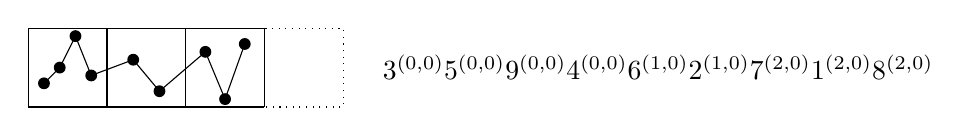
\begin{tikzpicture}
\def\xs{1.0}
\def\ys{1.0}
\def\ps{0.75}
\draw (0,0) grid[xscale=\xs,yscale=\ys] (3, 1);
\draw[dotted] (3*\xs,0) rectangle (4*\xs,1*\xs);
\coordinate (p0) at (0.2*\xs,0.30000000000000004*\ys);
\coordinate (p1) at (0.4*\xs,0.5*\ys);
\coordinate (p2) at (0.6000000000000001*\xs,0.9*\ys);
\coordinate (p3) at (0.8*\xs,0.4*\ys);
\coordinate (p4) at (1.3333333333333333*\xs,0.6000000000000001*\ys);
\coordinate (p5) at (1.6666666666666665*\xs,0.2*\ys);
\coordinate (p6) at (2.25*\xs,0.7000000000000001*\ys);
\coordinate (p7) at (2.5*\xs,0.1*\ys);
\coordinate (p8) at (2.75*\xs,0.8*\ys);
\draw (p0)--(p1)--(p2)--(p3)--(p4)--(p5)--(p6)--(p7)--(p8);
\fill (p0) circle (0.1*\ps);
\fill (p1) circle (0.1*\ps);
\fill (p2) circle (0.1*\ps);
\fill (p3) circle (0.1*\ps);
\fill (p4) circle (0.1*\ps);
\fill (p5) circle (0.1*\ps);
\fill (p6) circle (0.1*\ps);
\fill (p7) circle (0.1*\ps);
\fill (p8) circle (0.1*\ps);
\draw (8,0.5) node {$3^{(0,0)}5^{(0,0)}9^{(0,0)}4^{(0,0)}6^{(1,0)}2^{(1,0)}7^{(2,0)}1^{(2,0)}8^{(2,0)}$};
\end{tikzpicture}

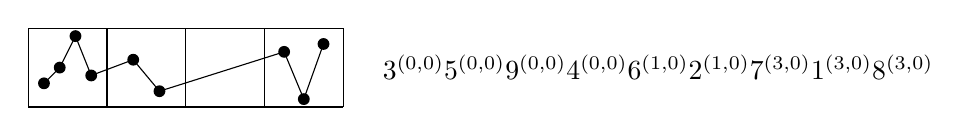
\begin{tikzpicture}
\def\xs{1.0}
\def\ys{1.0}
\def\ps{0.75}
\draw (0,0) grid[xscale=\xs,yscale=\ys] (4, 1);
\coordinate (p0) at (0.2*\xs,0.30000000000000004*\ys);
\coordinate (p1) at (0.4*\xs,0.5*\ys);
\coordinate (p2) at (0.6000000000000001*\xs,0.9*\ys);
\coordinate (p3) at (0.8*\xs,0.4*\ys);
\coordinate (p4) at (1.3333333333333333*\xs,0.6000000000000001*\ys);
\coordinate (p5) at (1.6666666666666665*\xs,0.2*\ys);
\coordinate (p6) at (1+2.25*\xs,0.7000000000000001*\ys);
\coordinate (p7) at (1+2.5*\xs,0.1*\ys);
\coordinate (p8) at (1+2.75*\xs,0.8*\ys);
\draw (p0)--(p1)--(p2)--(p3)--(p4)--(p5)--(p6)--(p7)--(p8);
\fill (p0) circle (0.1*\ps);
\fill (p1) circle (0.1*\ps);
\fill (p2) circle (0.1*\ps);
\fill (p3) circle (0.1*\ps);
\fill (p4) circle (0.1*\ps);
\fill (p5) circle (0.1*\ps);
\fill (p6) circle (0.1*\ps);
\fill (p7) circle (0.1*\ps);
\fill (p8) circle (0.1*\ps);
\draw (8,0.5) node {$3^{(0,0)}5^{(0,0)}9^{(0,0)}4^{(0,0)}6^{(1,0)}2^{(1,0)}7^{(3,0)}1^{(3,0)}8^{(3,0)}$};
\end{tikzpicture}

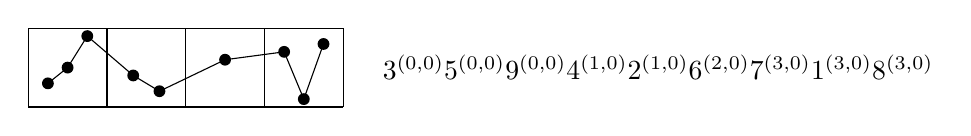
\begin{tikzpicture}
\def\xs{1.0}
\def\ys{1.0}
\def\ps{0.75}
\draw (0,0) grid[xscale=\xs,yscale=\ys] (4, 1);
\coordinate (p0) at (0.25*\xs,0.30000000000000004*\ys);
\coordinate (p1) at (0.5*\xs,0.5*\ys);
\coordinate (p2) at (0.75*\xs,0.9*\ys);
\coordinate (p3) at (1.3333333333333333*\xs,0.4*\ys);
\coordinate (p4) at (1.6666666666666665*\xs,0.2*\ys);
\coordinate (p5) at (2.5*\xs,0.6000000000000001*\ys);
\coordinate (p6) at (3.25*\xs,0.7000000000000001*\ys);
\coordinate (p7) at (3.5*\xs,0.1*\ys);
\coordinate (p8) at (3.75*\xs,0.8*\ys);
\draw (p0)--(p1)--(p2)--(p3)--(p4)--(p5)--(p6)--(p7)--(p8);
\fill (p0) circle (0.1*\ps);
\fill (p1) circle (0.1*\ps);
\fill (p2) circle (0.1*\ps);
\fill (p3) circle (0.1*\ps);
\fill (p4) circle (0.1*\ps);
\fill (p5) circle (0.1*\ps);
\fill (p6) circle (0.1*\ps);
\fill (p7) circle (0.1*\ps);
\fill (p8) circle (0.1*\ps);
\draw (8,0.5) node {$3^{(0,0)}5^{(0,0)}9^{(0,0)}4^{(1,0)}2^{(1,0)}6^{(2,0)}7^{(3,0)}1^{(3,0)}8^{(3,0)}$};
\end{tikzpicture}

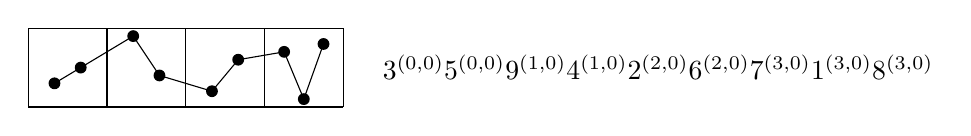
\begin{tikzpicture}
\def\xs{1.0}
\def\ys{1.0}
\def\ps{0.75}
\draw (0,0) grid[xscale=\xs,yscale=\ys] (4, 1);
\coordinate (p0) at (0.3333333333333333*\xs,0.30000000000000004*\ys);
\coordinate (p1) at (0.6666666666666666*\xs,0.5*\ys);
\coordinate (p2) at (1.3333333333333333*\xs,0.9*\ys);
\coordinate (p3) at (1.6666666666666665*\xs,0.4*\ys);
\coordinate (p4) at (2.3333333333333335*\xs,0.2*\ys);
\coordinate (p5) at (2.6666666666666665*\xs,0.6000000000000001*\ys);
\coordinate (p6) at (3.25*\xs,0.7000000000000001*\ys);
\coordinate (p7) at (3.5*\xs,0.1*\ys);
\coordinate (p8) at (3.75*\xs,0.8*\ys);
\draw (p0)--(p1)--(p2)--(p3)--(p4)--(p5)--(p6)--(p7)--(p8);
\fill (p0) circle (0.1*\ps);
\fill (p1) circle (0.1*\ps);
\fill (p2) circle (0.1*\ps);
\fill (p3) circle (0.1*\ps);
\fill (p4) circle (0.1*\ps);
\fill (p5) circle (0.1*\ps);
\fill (p6) circle (0.1*\ps);
\fill (p7) circle (0.1*\ps);
\fill (p8) circle (0.1*\ps);
\draw (8,0.5) node {$3^{(0,0)}5^{(0,0)}9^{(1,0)}4^{(1,0)}2^{(2,0)}6^{(2,0)}7^{(3,0)}1^{(3,0)}8^{(3,0)}$};
\end{tikzpicture}

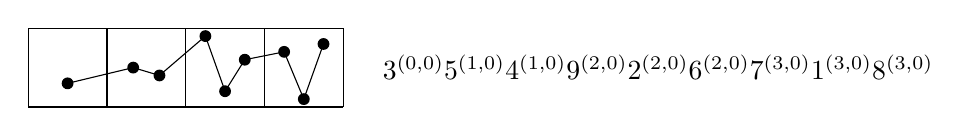
\begin{tikzpicture}
\def\xs{1.0}
\def\ys{1.0}
\def\ps{0.75}
\draw (0,0) grid[xscale=\xs,yscale=\ys] (4, 1);
\coordinate (p0) at (0.5*\xs,0.30000000000000004*\ys);
\coordinate (p1) at (1.3333333333333333*\xs,0.5*\ys);
\coordinate (p2) at (1.6666666666666665*\xs,0.4*\ys);
\coordinate (p3) at (2.25*\xs,0.9*\ys);
\coordinate (p4) at (2.5*\xs,0.2*\ys);
\coordinate (p5) at (2.75*\xs,0.6000000000000001*\ys);
\coordinate (p6) at (3.25*\xs,0.7000000000000001*\ys);
\coordinate (p7) at (3.5*\xs,0.1*\ys);
\coordinate (p8) at (3.75*\xs,0.8*\ys);
\draw (p0)--(p1)--(p2)--(p3)--(p4)--(p5)--(p6)--(p7)--(p8);
\fill (p0) circle (0.1*\ps);
\fill (p1) circle (0.1*\ps);
\fill (p2) circle (0.1*\ps);
\fill (p3) circle (0.1*\ps);
\fill (p4) circle (0.1*\ps);
\fill (p5) circle (0.1*\ps);
\fill (p6) circle (0.1*\ps);
\fill (p7) circle (0.1*\ps);
\fill (p8) circle (0.1*\ps);
\draw (8,0.5) node {$3^{(0,0)}5^{(1,0)}4^{(1,0)}9^{(2,0)}2^{(2,0)}6^{(2,0)}7^{(3,0)}1^{(3,0)}8^{(3,0)}$};
\end{tikzpicture}

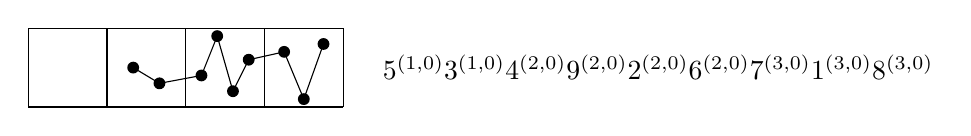
\begin{tikzpicture}
\def\xs{1.0}
\def\ys{1.0}
\def\ps{0.75}
\draw (0,0) grid[xscale=\xs,yscale=\ys] (4, 1);
\coordinate (p0) at (1.3333333333333333*\xs,0.5*\ys);
\coordinate (p1) at (1.6666666666666665*\xs,0.30000000000000004*\ys);
\coordinate (p2) at (2.2*\xs,0.4*\ys);
\coordinate (p3) at (2.4*\xs,0.9*\ys);
\coordinate (p4) at (2.6*\xs,0.2*\ys);
\coordinate (p5) at (2.8*\xs,0.6000000000000001*\ys);
\coordinate (p6) at (3.25*\xs,0.7000000000000001*\ys);
\coordinate (p7) at (3.5*\xs,0.1*\ys);
\coordinate (p8) at (3.75*\xs,0.8*\ys);
\draw (p0)--(p1)--(p2)--(p3)--(p4)--(p5)--(p6)--(p7)--(p8);
\fill (p0) circle (0.1*\ps);
\fill (p1) circle (0.1*\ps);
\fill (p2) circle (0.1*\ps);
\fill (p3) circle (0.1*\ps);
\fill (p4) circle (0.1*\ps);
\fill (p5) circle (0.1*\ps);
\fill (p6) circle (0.1*\ps);
\fill (p7) circle (0.1*\ps);
\fill (p8) circle (0.1*\ps);
\draw (8,0.5) node {$5^{(1,0)}3^{(1,0)}4^{(2,0)}9^{(2,0)}2^{(2,0)}6^{(2,0)}7^{(3,0)}1^{(3,0)}8^{(3,0)}$};
\end{tikzpicture}

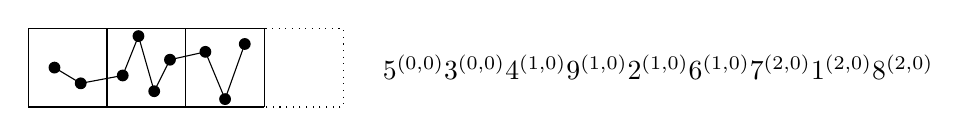
\begin{tikzpicture}
\def\xs{1.0}
\def\ys{1.0}
\def\ps{0.75}
\draw (0,0) grid[xscale=\xs,yscale=\ys] (3, 1);
\draw[dotted] (3*\xs,0) rectangle (4*\xs,1*\xs);
\coordinate (p0) at (-1+1.3333333333333333*\xs,0.5*\ys);
\coordinate (p1) at (-1+1.6666666666666665*\xs,0.30000000000000004*\ys);
\coordinate (p2) at (-1+2.2*\xs,0.4*\ys);
\coordinate (p3) at (-1+2.4*\xs,0.9*\ys);
\coordinate (p4) at (-1+2.6*\xs,0.2*\ys);
\coordinate (p5) at (-1+2.8*\xs,0.6000000000000001*\ys);
\coordinate (p6) at (-1+3.25*\xs,0.7000000000000001*\ys);
\coordinate (p7) at (-1+3.5*\xs,0.1*\ys);
\coordinate (p8) at (-1+3.75*\xs,0.8*\ys);
\draw (p0)--(p1)--(p2)--(p3)--(p4)--(p5)--(p6)--(p7)--(p8);
\fill (p0) circle (0.1*\ps);
\fill (p1) circle (0.1*\ps);
\fill (p2) circle (0.1*\ps);
\fill (p3) circle (0.1*\ps);
\fill (p4) circle (0.1*\ps);
\fill (p5) circle (0.1*\ps);
\fill (p6) circle (0.1*\ps);
\fill (p7) circle (0.1*\ps);
\fill (p8) circle (0.1*\ps);
\draw (8,0.5) node {$5^{(0,0)}3^{(0,0)}4^{(1,0)}9^{(1,0)}2^{(1,0)}6^{(1,0)}7^{(2,0)}1^{(2,0)}8^{(2,0)}$};
\end{tikzpicture}

\begin{tikzpicture}\end{tikzpicture}
    \caption{The sliding of $3594^{(0,0)}62^{(1,0)}718^{(2,0)}$.}
    \label{fig:slide_gp_example}
\end{figure}

\begin{definition}\label{def:slidable}
A pair of tilings
\[
    (\mathcal{T}_1,\mathcal{T}_2) = \left(\left((c,1), \mathcal{O}_1, \set{\mathcal{R}_1,\ldots,\mathcal{R}_k}\right), \left((c,1), \mathcal{O}_2, \set{\mathcal{R}'_1,\ldots,\mathcal{R}'_k}\right)\right)
\]
is \emph{slidable} if the following conditions are satisfied.
\begin{itemize}
    \item The tilings share requirements, that is $\set{\mathcal{R}_1,\ldots,\mathcal{R}_k}=\set{\mathcal{R}'_1,\ldots,\mathcal{R}'_k}$.
    \item No gridded permutation in $\mathcal{R}_1 \cup \cdots \cup \mathcal{R}_k$ has positions in columns $0$ and $1$.
    \item There exists an $n>1$ such that the obstructions $12\cdots n^{(0,0)}, 12\cdots (n-1)^{(0,0)}n^{(1,0)}$ and $12^{(1,0)}$ belong to $\mathcal{O}_1$, $12\cdots n^{(1,0)}, 1^{(0,0)}23\cdots n^{(1,0)}$ and $12^{(0,0)}$ belong to $\mathcal{O}_2$ and no other obstructions that are entirely within columns $0$ and $1$ belong to either $\mathcal{O}_1$ or $\mathcal{O}_2$.
    \item For any obstruction $\pi = \pi_1^{(x_1,0)}\pi_2^{(x_2,0)}\cdots\pi_n^{(x_w,0)} \in \mathcal{O}_1$ with at least one element outside columns $0$ and $1$ the subsequence $\sseq{\cset{i \in [w]}{x_i \in \set{0,1}}}{\pi}$ is either empty or in 
    \[
         \cset{j(j+1)^{(0,0)}, j^{(0,0)}(j+1)^{(1,0)}, j^{(0,0)},j^{(1,0)}}{j\in\Z^+}.
    \]
    Similarly, for $\mathcal{O}_2$, the subsequence must be either empty or in 
    \[
         \cset{j(j+1)^{(1,0)}, j^{(0,0)}(j+1)^{(1,0)}, j^{(0,0)},j^{(1,0)}}{j\in\Z^+}.
    \]
    \item Any obstruction entirely outside columns $0$ and $1$ in $\mathcal{O}_1$ must also exist in $\mathcal{O}_2$ and vice versa.
    \item Let $o_1 = \pi_1^{(0,0)}\pi_2^{(x_2,0)}\cdots\pi_s^{(x_s,0)}$ and $o_2 = \pi_1^{(1,0)}\pi_2^{(x_2,0)}\cdots\pi_s^{(x_s,0)}$ where $x_2,s > 1$ then $o_1 \in \mathcal{O}_1$, $o_2 \in \mathcal{O}_1$, $o_1 \in \mathcal{O}_2$ and $o_2 \in \mathcal{O}_2$ are equivalent. That is, any crossing obstruction with one point in the first two columns must exist in both tilings and with that point in both columns.
    \item Let \begin{align*}o_1 &= \pi_1^{(0,0)}\pi_2^{(0,0)}\pi_3^{(x_3,0)}\cdots\pi_s^{(x_s,0)}\\o_2 &= \pi_1^{(0,0)}\pi_2^{(1,0)}\pi_3^{(x_3,0)}\cdots\pi_s^{(x_s,0)}\\o_3 &= \pi_1^{(1,0)}\pi_2^{(1,0)}\pi_3^{(x_3,0)}\cdots\pi_s^{(x_s,0)}\end{align*} where $s > 2$, $x_3 > 1$ and $\pi_1 + 1 = \pi_2$, then $o_1 \in \mathcal{O}_1$, $o_2 \in \mathcal{O}_1$, $o_2 \in \mathcal{O}_2$ and $o_3 \in \mathcal{O}_2$ are equivalent. That is, any crossing obstruction with $j(j+1)$ in the first two columns (and at least one point outside of those columns) must exists in both tilings where $j(j+1)$ has been spread between the first two columns in all possible ways, excluding the one that collides with the $12$ obstruction.
\end{itemize}
\end{definition}

An example of two slidable tilings can be seen in \FigureRef{fig:slidable_tilings}.

\begin{figure}[ht]
    \centering
    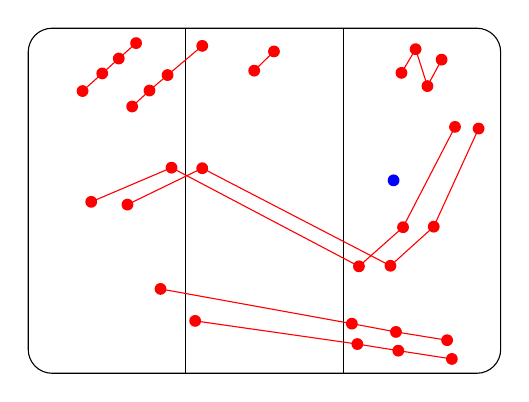
\begin{tikzpicture}[scale=1, every node/.style={scale=1}]
\def\xscale{1.0} % Horizontal scale factor
\def\yscale{0.7} % Vertical scale factor
\def\spnt{0.075} % Size of smaller points
\def\lpnt{0.125} % Size of larger points
\draw[rounded corners=2ex] (0,0) rectangle (6*\xscale,6.26*\yscale);
\draw (2.0*\xscale, 6.26*\yscale) -- (2.0*\xscale, 0);
\draw (4.0*\xscale, 6.26*\yscale) -- (4.0*\xscale, 0);
\fill[red] (2.87*\xscale, 5.49*\yscale) circle (\spnt);
\fill[red] (3.1209520279019056*\xscale, 5.838779282906702*\yscale) circle (\spnt);
\draw[red] (2.87*\xscale, 5.49*\yscale) -- (3.1209520279019056*\xscale,5.838779282906702*\yscale);
\fill[red] (0.69*\xscale, 5.12*\yscale) circle (\spnt);
\fill[red] (0.94*\xscale, 5.44*\yscale) circle (\spnt);
\fill[red] (1.15*\xscale, 5.71*\yscale) circle (\spnt);
\fill[red] (1.37*\xscale, 5.99*\yscale) circle (\spnt);
\draw[red] (0.69*\xscale, 5.12*\yscale) -- (0.94*\xscale,5.44*\yscale) -- (1.15*\xscale,5.71*\yscale) -- (1.37*\xscale,5.99*\yscale);
\fill[red] (1.32*\xscale, 4.84*\yscale) circle (\spnt);
\fill[red] (1.54*\xscale, 5.13*\yscale) circle (\spnt);
\fill[red] (1.77*\xscale, 5.41*\yscale) circle (\spnt);
\fill[red] (2.21*\xscale, 5.94*\yscale) circle (\spnt);
\draw[red] (1.32*\xscale, 4.84*\yscale) -- (1.54*\xscale,5.13*\yscale) -- (1.77*\xscale,5.41*\yscale) -- (2.21*\xscale,5.94*\yscale);
\fill[red] (4.74*\xscale, 5.45*\yscale) circle (\spnt);
\fill[red] (4.92*\xscale, 5.88*\yscale) circle (\spnt);
\fill[red] (5.07*\xscale, 5.21*\yscale) circle (\spnt);
\fill[red] (5.25*\xscale, 5.69*\yscale) circle (\spnt);
\draw[red] (4.74*\xscale, 5.45*\yscale) -- (4.92*\xscale,5.88*\yscale) -- (5.07*\xscale,5.21*\yscale) -- (5.25*\xscale,5.69*\yscale);
\fill[red] (1.68*\xscale, 1.53*\yscale) circle (\spnt);
\fill[red] (4.11*\xscale, 0.9*\yscale) circle (\spnt);
\fill[red] (4.67*\xscale, 0.75*\yscale) circle (\spnt);
\fill[red] (5.32*\xscale, 0.6*\yscale) circle (\spnt);
\draw[red] (1.68*\xscale, 1.53*\yscale) -- (4.11*\xscale,0.9*\yscale) -- (4.67*\xscale,0.75*\yscale) -- (5.32*\xscale,0.6*\yscale);
\fill[red] (2.12*\xscale, 0.95*\yscale) circle (\spnt);
\fill[red] (4.18*\xscale, 0.53*\yscale) circle (\spnt);
\fill[red] (4.7*\xscale, 0.41*\yscale) circle (\spnt);
\fill[red] (5.38*\xscale, 0.26*\yscale) circle (\spnt);
\draw[red] (2.12*\xscale, 0.95*\yscale) -- (4.18*\xscale,0.53*\yscale) -- (4.7*\xscale,0.41*\yscale) -- (5.38*\xscale,0.26*\yscale);
\fill[red] (0.8*\xscale, 3.11*\yscale) circle (\spnt);
\fill[red] (1.82*\xscale, 3.73*\yscale) circle (\spnt);
\fill[red] (4.2*\xscale, 1.94*\yscale) circle (\spnt);
\fill[red] (4.76*\xscale, 2.65*\yscale) circle (\spnt);
\fill[red] (5.42*\xscale, 4.47*\yscale) circle (\spnt);
\draw[red] (0.8*\xscale, 3.11*\yscale) -- (1.82*\xscale,3.73*\yscale) -- (4.2*\xscale,1.94*\yscale) -- (4.76*\xscale,2.65*\yscale) -- (5.42*\xscale,4.47*\yscale);
\fill[red] (1.26*\xscale, 3.06*\yscale) circle (\spnt);
\fill[red] (2.21*\xscale, 3.72*\yscale) circle (\spnt);
\fill[red] (4.6*\xscale, 1.95*\yscale) circle (\spnt);
\fill[red] (5.15*\xscale, 2.66*\yscale) circle (\spnt);
\fill[red] (5.72*\xscale, 4.44*\yscale) circle (\spnt);
\draw[red] (1.26*\xscale, 3.06*\yscale) -- (2.21*\xscale,3.72*\yscale) -- (4.6*\xscale,1.95*\yscale) -- (5.15*\xscale,2.66*\yscale) -- (5.72*\xscale,4.44*\yscale);
\fill[blue] (4.64*\xscale, 3.5*\yscale) circle (\spnt);
\end{tikzpicture}
\hspace{0.5cm}
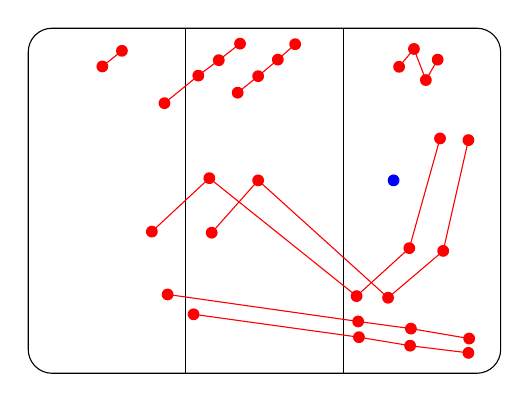
\begin{tikzpicture}[scale=1, every node/.style={scale=1}]
\def\xscale{1.0} % Horizontal scale factor
\def\yscale{0.7} % Vertical scale factor
\def\spnt{0.075} % Size of smaller points
\def\lpnt{0.125} % Size of larger points
\draw[rounded corners=2ex] (0,0) rectangle (6*\xscale,6.26*\yscale);
\draw (2.0*\xscale, 6.26*\yscale) -- (2.0*\xscale, 0);
\draw (4.0*\xscale, 6.26*\yscale) -- (4.0*\xscale, 0);
\fill[red] (0.9413254253242579*\xscale, 5.5665123438541855*\yscale) circle (\spnt);
\fill[red] (1.19*\xscale, 5.85*\yscale) circle (\spnt);
\draw[red] (0.9413254253242579*\xscale, 5.5665123438541855*\yscale) -- (1.19*\xscale,5.85*\yscale);
\fill[red] (1.73*\xscale, 4.9*\yscale) circle (\spnt);
\fill[red] (2.16*\xscale, 5.4*\yscale) circle (\spnt);
\fill[red] (2.42*\xscale, 5.68*\yscale) circle (\spnt);
\fill[red] (2.69*\xscale, 5.98*\yscale) circle (\spnt);
\draw[red] (1.73*\xscale, 4.9*\yscale) -- (2.16*\xscale,5.4*\yscale) -- (2.42*\xscale,5.68*\yscale) -- (2.69*\xscale,5.98*\yscale);
\fill[red] (2.66*\xscale, 5.09*\yscale) circle (\spnt);
\fill[red] (2.92*\xscale, 5.39*\yscale) circle (\spnt);
\fill[red] (3.17*\xscale, 5.69*\yscale) circle (\spnt);
\fill[red] (3.39*\xscale, 5.97*\yscale) circle (\spnt);
\draw[red] (2.66*\xscale, 5.09*\yscale) -- (2.92*\xscale,5.39*\yscale) -- (3.17*\xscale,5.69*\yscale) -- (3.39*\xscale,5.97*\yscale);
\fill[red] (4.71*\xscale, 5.56*\yscale) circle (\spnt);
\fill[red] (4.898395663501238*\xscale, 5.884152285333065*\yscale) circle (\spnt);
\fill[red] (5.05*\xscale, 5.32*\yscale) circle (\spnt);
\fill[red] (5.2*\xscale, 5.69*\yscale) circle (\spnt);
\draw[red] (4.71*\xscale, 5.56*\yscale) -- (4.898395663501238*\xscale,5.884152285333065*\yscale) -- (5.05*\xscale,5.32*\yscale) -- (5.2*\xscale,5.69*\yscale);
\fill[red] (1.77*\xscale, 1.43*\yscale) circle (\spnt);
\fill[red] (4.19*\xscale, 0.94*\yscale) circle (\spnt);
\fill[red] (4.86*\xscale, 0.81*\yscale) circle (\spnt);
\fill[red] (5.6*\xscale, 0.63*\yscale) circle (\spnt);
\draw[red] (1.77*\xscale, 1.43*\yscale) -- (4.19*\xscale,0.94*\yscale) -- (4.86*\xscale,0.81*\yscale) -- (5.6*\xscale,0.63*\yscale);
\fill[red] (2.1*\xscale, 1.07*\yscale) circle (\spnt);
\fill[red] (4.2*\xscale, 0.6546404918137944*\yscale) circle (\spnt);
\fill[red] (4.85*\xscale, 0.5*\yscale) circle (\spnt);
\fill[red] (5.59*\xscale, 0.37*\yscale) circle (\spnt);
\draw[red] (2.1*\xscale, 1.07*\yscale) -- (4.2*\xscale,0.6546404918137944*\yscale) -- (4.85*\xscale,0.5*\yscale) -- (5.59*\xscale,0.37*\yscale);
\fill[red] (1.57*\xscale, 2.57*\yscale) circle (\spnt);
\fill[red] (2.3*\xscale, 3.54*\yscale) circle (\spnt);
\fill[red] (4.17*\xscale, 1.4*\yscale) circle (\spnt);
\fill[red] (4.84*\xscale, 2.27*\yscale) circle (\spnt);
\fill[red] (5.23*\xscale, 4.26*\yscale) circle (\spnt);
\draw[red] (1.57*\xscale, 2.57*\yscale) -- (2.3*\xscale,3.54*\yscale) -- (4.17*\xscale,1.4*\yscale) -- (4.84*\xscale,2.27*\yscale) -- (5.23*\xscale,4.26*\yscale);
\fill[red] (2.33*\xscale, 2.55*\yscale) circle (\spnt);
\fill[red] (2.92*\xscale, 3.5*\yscale) circle (\spnt);
\fill[red] (4.57*\xscale, 1.37*\yscale) circle (\spnt);
\fill[red] (5.27*\xscale, 2.22*\yscale) circle (\spnt);
\fill[red] (5.59*\xscale, 4.23*\yscale) circle (\spnt);
\draw[red] (2.33*\xscale, 2.55*\yscale) -- (2.92*\xscale,3.5*\yscale) -- (4.57*\xscale,1.37*\yscale) -- (5.27*\xscale,2.22*\yscale) -- (5.59*\xscale,4.23*\yscale);
\fill[blue] (4.64*\xscale, 3.5*\yscale) circle (\spnt);
\end{tikzpicture}
    \caption{Typical slidable tilings.}
    \label{fig:slidable_tilings}
\end{figure}

\begin{lemma}\label{lem:slidemap}
Let $(\mathcal{T}_1,\mathcal{T}_2)$ be slidable and $i \in \N$, then $\Upsilon(\pi) \in \textsf{Grid}_i(\mathcal{T}_2)$ for every $\pi \in \textsf{Grid}_i(\mathcal{T}_1)$.
\end{lemma}
\begin{proof}
If $\pi$ contains no elements within the first two columns it is mapped to itself and since the tilings share requirements and are identical outside the first two columns then $\Upsilon(\pi) \in \textsf{Grid}_i(\mathcal{T}_2)$. If $\pi$ contains no elements in column $1$ then whatever is in column $0$ is moved to column $1$. Since $\pi$ avoided $12\dotsm n$ in column $0$ it will also do so in column $1$ once moved and any crossing obstruction in $\mathcal{T}_2$ with one or two points in column $1$ would have existed with those points in column $0$ in $\mathcal{T}_1$ and therefore $\Upsilon(\pi) \in \textsf{Grid}_i(\mathcal{T}_2)$.

Now suppose $\pi$ has elements in column $1$. By the end of the mapping all columns are shifted one to the left but we will refer to their indices before the shift in the mapped tiling. Note that the mapping is defined by placing elements in-order into column $1$ so we will never form an increasing pattern there. 

Suppose after a single step in the map that we form the first $12\cdots n$ (spread in any way across the first $3$ columns). Note that it can contain at most one point in column $1$ as that column is decreasing.

If the $12\cdots n$ pattern does contain the newly moved point in column $1$ and not the one we just moved to column $2$, then the pattern must have been there before the step was taken.

\begin{center}
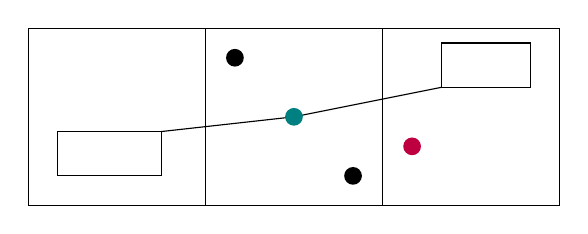
\begin{tikzpicture}[scale=0.75]
    \draw (2.25,1.25) -- (4.5,1.5) -- (7,2);
    \draw (0,0) rectangle (3,3);
    \draw (3,0) rectangle (6,3);
    \draw (6,0) rectangle (9,3);
    \fill (3.5,2.5) circle (0.15);
    \fill[teal] (4.5,1.5) circle (0.15);
    \fill (5.5,0.5) circle (0.15);
    \draw (0.5,0.5) rectangle (2.25,1.25);
    \fill[purple] (6.5,1) circle (0.15);
    \draw (7,2) rectangle (8.5,2.75);
\end{tikzpicture}
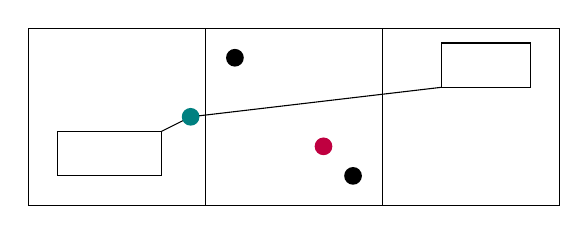
\begin{tikzpicture}[scale=0.75]
    \draw (2.25,1.25) -- (2.75,1.5) -- (7,2);
    \draw (0,0) rectangle (3,3);
    \draw (3,0) rectangle (6,3);
    \draw (6,0) rectangle (9,3);
    \fill (3.5,2.5) circle (0.15);
    \fill[teal] (2.75,1.5) circle (0.15);
    \fill (5.5,0.5) circle (0.15);
    \draw (0.5,0.5) rectangle (2.25,1.25);
    \fill[purple] (5,1) circle (0.15);
    \draw (7,2) rectangle (8.5,2.75);
\end{tikzpicture}
\end{center}

Suppose this pattern includes the newly moved element in column $2$ and no elements in column $1$ then the pattern must have existed before regardless of whether the new element in column $2$ was the smallest element in column $1$ before the move or not.

\begin{center}
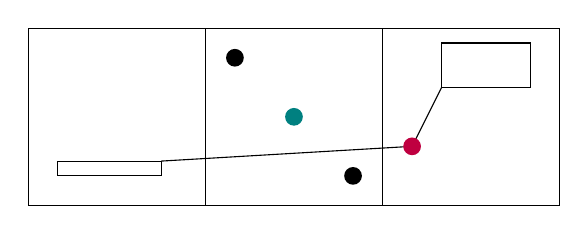
\begin{tikzpicture}[scale=0.75]
    \draw (2.25,0.75) -- (6.5,1) -- (7,2);
    \draw (0,0) rectangle (3,3);
    \draw (3,0) rectangle (6,3);
    \draw (6,0) rectangle (9,3);
    \fill (3.5,2.5) circle (0.15);
    \fill[teal] (4.5,1.5) circle (0.15);
    \fill (5.5,0.5) circle (0.15);
    \draw (0.5,0.5) rectangle (2.25,0.75);
    \fill[purple] (6.5,1) circle (0.15);
    \draw (7,2) rectangle (8.5,2.75);
\end{tikzpicture}
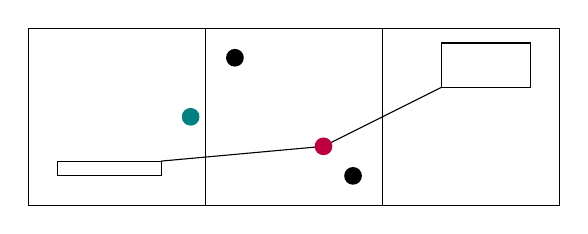
\begin{tikzpicture}[scale=0.75]
    \draw (2.25,0.75) -- (5,1) -- (7,2);
    \draw (0,0) rectangle (3,3);
    \draw (3,0) rectangle (6,3);
    \draw (6,0) rectangle (9,3);
    \fill (3.5,2.5) circle (0.15);
    \fill[teal] (2.75,1.5) circle (0.15);
    \fill (5.5,0.5) circle (0.15);
    \draw (0.5,0.5) rectangle (2.25,0.75);
    \fill[purple] (5,1) circle (0.15);
    \draw (7,2) rectangle (8.5,2.75);
\end{tikzpicture}
\end{center}

Finally suppose the pattern involves elements from both columns $1$ and $2$. Here two scenario can arise. One were the pattern involves both moved elements and the other only the one moved to column $2$. In the first one the pattern remains as we move both points together when we backtrack.

\begin{center}
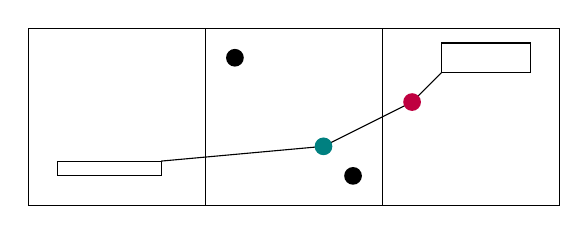
\begin{tikzpicture}[scale=0.75]
    \draw (2.25,0.75) -- (5,1) -- (6.5,1.75) -- (7,2.25);
    \draw (0,0) rectangle (3,3);
    \draw (3,0) rectangle (6,3);
    \draw (6,0) rectangle (9,3);
    \fill (3.5,2.5) circle (0.15);
    \fill[teal] (5,1) circle (0.15);
    \fill (5.5,0.5) circle (0.15);
    \draw (0.5,0.5) rectangle (2.25,0.75);
    \fill[purple] (6.5,1.75) circle (0.15);
    \draw (7,2.25) rectangle (8.5,2.75);
\end{tikzpicture}
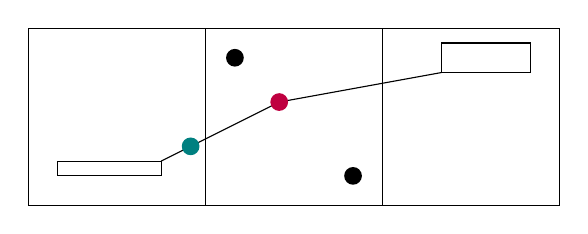
\begin{tikzpicture}[scale=0.75]
    \draw (2.25,0.75) -- (2.75,1) -- (4.25,1.75) -- (7,2.25);
    \draw (0,0) rectangle (3,3);
    \draw (3,0) rectangle (6,3);
    \draw (6,0) rectangle (9,3);
    \fill (3.5,2.5) circle (0.15);
    \fill[teal] (2.75,1) circle (0.15);
    \fill (5.5,0.5) circle (0.15);
    \draw (0.5,0.5) rectangle (2.25,0.75);
    \fill[purple] (4.25,1.75) circle (0.15);
    \draw (7,2.25) rectangle (8.5,2.75);
\end{tikzpicture}
\end{center}

In the latter, there is a smaller element in column $1$ than the moved one that belongs to the pattern. When we go back, the moved element goes back from column $1$ to column $0$ but that is between the element in column $1$ that formed the pattern and the element that was moved to column $2$, preserving the pattern.

\begin{center}
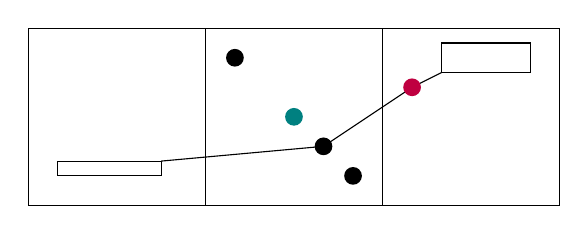
\begin{tikzpicture}[scale=0.75]
    \draw (2.25,0.75) -- (5,1) -- (6.5,2) -- (7,2.25);
    \draw (0,0) rectangle (3,3);
    \draw (3,0) rectangle (6,3);
    \draw (6,0) rectangle (9,3);
    \fill (5.5,0.5) circle (0.15);
    \fill (5,1) circle (0.15);
    \fill[teal] (4.5,1.5) circle (0.15);
    \fill[purple] (6.5,2) circle (0.15);
    \fill (3.5,2.5) circle (0.15);
    \draw (0.5,0.5) rectangle (2.25,0.75);
    \draw (7,2.25) rectangle (8.5,2.75);
\end{tikzpicture}
\begin{tikzpicture}[scale=0.75]
    \draw (2.25,0.75) -- (2.75,1.5) -- (4,2) -- (7,2.25);
    \draw (0,0) rectangle (3,3);
    \draw (3,0) rectangle (6,3);
    \draw (6,0) rectangle (9,3);
    \fill (5.5,0.5) circle (0.15);
    \fill (5,1) circle (0.15);
    \fill[teal] (2.75,1.5) circle (0.15);
    \fill[purple] (4,2) circle (0.15);
    \fill (3.5,2.5) circle (0.15);
    \draw (0.5,0.5) rectangle (2.25,0.75);
    \draw (7,2.25) rectangle (8.5,2.75);
\end{tikzpicture}
\end{center}

In the case of the first crossing obstructions forming for the first time with one element in the first 3 columns and some outside, then wherever that element was before must have been an occurrence of that pattern as well.

Now suppose we form the crossing pattern with the elements $k(k+1)$ in the first three columns (spread in any way) for the first time. This can happen in several ways. Note that the two increasing elements can not both be in column $1$ as it is always decreasing.

Suppose the $k(k+1)$ part in the first $3$ columns occurs between the first two, then the pattern must have existed before with $k(k+1)$ in column $0$.

\begin{center}
\begin{tikzpicture}[scale=0.63]
    \coordinate (a1) at (5.5,0.5);
    \coordinate (a2) at (2.75,1);
    \coordinate (a3) at (4.5,1.5);
    \coordinate (a4) at (6.25,2);
    \coordinate (a5) at (3.5,2.5);
    \draw (a2) -- (a3) -- (9.25,1.5);
    \draw (0,0) rectangle (3,3);
    \draw (3,0) rectangle (6,3);
    \draw (6,0) rectangle (9,3);
    \draw (9,0) rectangle (12,3);
    \fill (a1) circle (0.15);
    \fill (a2) circle (0.15);
    \fill[teal] (a3) circle (0.15);
    \fill[purple] (a4) circle (0.15);
    \fill (a5) circle (0.15);
    \draw (9.25,0.25) rectangle (11.75,2.75);
\end{tikzpicture}
\begin{tikzpicture}[scale=0.63]
    \coordinate (a1) at (5.5,0.5);
    \coordinate (a2) at (2.25,1);
    \coordinate (a3) at (2.75,1.5);
    \coordinate (a4) at (4,2);
    \coordinate (a5) at (3.5,2.5);
    \draw (a2) -- (a3) -- (9.25,1.5);
    \draw (0,0) rectangle (3,3);
    \draw (3,0) rectangle (6,3);
    \draw (6,0) rectangle (9,3);
    \draw (9,0) rectangle (12,3);
    \fill (a1) circle (0.15);
    \fill (a2) circle (0.15);
    \fill[teal] (a3) circle (0.15);
    \fill[purple] (a4) circle (0.15);
    \fill (a5) circle (0.15);
    \draw (9.25,0.25) rectangle (11.75,2.75);
\end{tikzpicture}
\end{center}

If the pattern occurs with $k(k+1)$ in columns $0$ and $2$, then it must have existed with $k(k+1)$ in columns $0$ and $1$ before.

\begin{center}
\begin{tikzpicture}[scale=0.63]
    \coordinate (a1) at (5.5,0.5);
    \coordinate (a2) at (5,1);
    \coordinate (a3) at (2.75,1.5);
    \coordinate (a4) at (6.25,2);
    \coordinate (a5) at (3.5,2.5);
    \draw (a3) -- (a4) -- (9.25,2);
    \draw (0,0) rectangle (3,3);
    \draw (3,0) rectangle (6,3);
    \draw (6,0) rectangle (9,3);
    \draw (9,0) rectangle (12,3);
    \fill (a1) circle (0.15);
    \fill[teal] (a2) circle (0.15);
    \fill (a3) circle (0.15);
    \fill[purple] (a4) circle (0.15);
    \fill (a5) circle (0.15);
    \draw (9.25,0.25) rectangle (11.75,2.75);
\end{tikzpicture}
\begin{tikzpicture}[scale=0.63]
    \coordinate (a1) at (5.5,0.5);
    \coordinate (a2) at (2.75,1);
    \coordinate (a3) at (2.25,1.5);
    \coordinate (a4) at (4,2);
    \coordinate (a5) at (3.5,2.5);
    \draw (a3) -- (a4) -- (9.25,2);
    \draw (0,0) rectangle (3,3);
    \draw (3,0) rectangle (6,3);
    \draw (6,0) rectangle (9,3);
    \draw (9,0) rectangle (12,3);
    \fill (a1) circle (0.15);
    \fill[teal] (a2) circle (0.15);
    \fill (a3) circle (0.15);
    \fill[purple] (a4) circle (0.15);
    \fill (a5) circle (0.15);
    \draw (9.25,0.25) rectangle (11.75,2.75);
\end{tikzpicture}
\end{center}

If the pattern occurs with $k(k+1)$ in columns $1$ and $2$ then, since they are adjacent in value and increasing, these must also be the two elements that were moved and therefore the pattern must have existed with $k(k+1)$ in columns $0$ and $1$ before.

\begin{center}
\begin{tikzpicture}[scale=0.63]
    \coordinate (a1) at (5.5,0.5);
    \coordinate (a2) at (5,1);
    \coordinate (a3) at (4.5,1.5);
    \coordinate (a4) at (6.25,2);
    \coordinate (a5) at (3.5,2.5);
    \draw (a3) -- (a4) -- (9.25,2);
    \draw (0,0) rectangle (3,3);
    \draw (3,0) rectangle (6,3);
    \draw (6,0) rectangle (9,3);
    \draw (9,0) rectangle (12,3);
    \fill (a1) circle (0.15);
    \fill (a2) circle (0.15);
    \fill[teal] (a3) circle (0.15);
    \fill[purple] (a4) circle (0.15);
    \fill (a5) circle (0.15);
    \draw (9.25,0.25) rectangle (11.75,2.75);
\end{tikzpicture}
\begin{tikzpicture}[scale=0.63]
    \coordinate (a1) at (5.5,0.5);
    \coordinate (a2) at (5,1);
    \coordinate (a3) at (2.75,1.5);
    \coordinate (a4) at (4,2);
    \coordinate (a5) at (3.5,2.5);
    \draw (a3) -- (a4) -- (9.25,2);
    \draw (0,0) rectangle (3,3);
    \draw (3,0) rectangle (6,3);
    \draw (6,0) rectangle (9,3);
    \draw (9,0) rectangle (12,3);
    \fill (a1) circle (0.15);
    \fill (a2) circle (0.15);
    \fill[teal] (a3) circle (0.15);
    \fill[purple] (a4) circle (0.15);
    \fill (a5) circle (0.15);
    \draw (9.25,0.25) rectangle (11.75,2.75);
\end{tikzpicture}
\end{center}

If the pattern occurs with $k(k+1)$ entirely within column $2$, then the pattern must have existed with $k(k+1)$ in columns $1$ and $2$ before.

\begin{center}
\begin{tikzpicture}[scale=0.63]
    \coordinate (a1) at (5.5,0.5);
    \coordinate (a2) at (5,1);
    \coordinate (a3) at (6.25,1.5);
    \coordinate (a4) at (6.75,2);
    \coordinate (a5) at (3.5,2.5);
    \draw (a3) -- (a4) -- (9.25,1.5);
    \draw (0,0) rectangle (3,3);
    \draw (3,0) rectangle (6,3);
    \draw (6,0) rectangle (9,3);
    \draw (9,0) rectangle (12,3);
    \fill (a1) circle (0.15);
    \fill[teal] (a2) circle (0.15);
    \fill[purple] (a3) circle (0.15);
    \fill (a4) circle (0.15);
    \fill (a5) circle (0.15);
    \draw (9.25,0.25) rectangle (11.75,2.75);
\end{tikzpicture}
\begin{tikzpicture}[scale=0.63]
    \coordinate (a1) at (5.5,0.5);
    \coordinate (a2) at (2.75,1);
    \coordinate (a3) at (4.5,1.5);
    \coordinate (a4) at (6.25,2);
    \coordinate (a5) at (3.5,2.5);
    \draw (a3) -- (a4) -- (9.25,1.5);
    \draw (0,0) rectangle (3,3);
    \draw (3,0) rectangle (6,3);
    \draw (6,0) rectangle (9,3);
    \draw (9,0) rectangle (12,3);
    \fill (a1) circle (0.15);
    \fill[teal] (a2) circle (0.15);
    \fill[purple] (a3) circle (0.15);
    \fill (a4) circle (0.15);
    \fill (a5) circle (0.15);
    \draw (9.25,0.25) rectangle (11.75,2.75);
\end{tikzpicture}
\end{center}

The trivial bijection of shifting the entire gridded permutation one column to the left (with column $0$ being depleted after the mapping) will not create any of these patterns. Since no obstruction from $\mathcal{T}_2$ can occur, $\Upsilon(\pi)$ is in $\textsf{Grid}_i(\mathcal{T}_2)$.
\end{proof}

\begin{definition}
Let $\pi = \pi_1^{(x_1,0)}\pi_2^{(x_2,0)}\cdots\pi_n^{(x_n,0)} \in \mathcal{G}^{(c,1)}_n$. We define \emph{inverse sliding} as the map $\Upsilon^{-1}: \mathcal{G}^{(c,1)}_n \to \mathcal{G}^{(c,1)}_n$ defined as follows.
\begin{enumerate}[a)]
    \item If $\pi$ has no elements in $(0,0)$, we move whatever is in $(1,0)$ to $(0,0)$ and we are done.
    \item If $\pi$ has elements in $(0,0)$, we start by shifting all elements one cell to the right and then we do the following until we have depleted the elements of $\pi$ in $(2,0)$:
    \begin{enumerate}[i.]
        \item If the leftmost element in $(2,0)$ is smaller than all elements in $(1,0)$, we move the leftmost element of $(1,0)$ to $(0,0)$ as the rightmost element and then we move the leftmost element of $(2,0)$ to $(1,0)$ as the rightmost element.
        \item If the leftmost element in $(2,0)$ has a smaller element in $(1,0)$, then we move the leftmost element in $(2,0)$ to the left of the largest element in $(1,0)$ that is smaller than it and that element is moved to be the rightmost element in $(0,0)$.
    \end{enumerate}
    Finally we shift all elements in $(3,0), (4,0), \ldots$ one cell to the left.
\end{enumerate}
\end{definition}

\begin{lemma}
Let $(\mathcal{T}_1,\mathcal{T}_2)$ be slidable and $i \in \N$, then $\Upsilon^{-1}(\pi) \in \textsf{Grid}_i(\mathcal{T}_1)$ for every $\pi \in \textsf{Grid}_i(\mathcal{T}_2)$.
\end{lemma}
\begin{proof}
The argument when $(0,0)$ is empty is an analog of the case in Lemma \ref{lem:slidemap} when $(1,0)$ is empty so we assume that $\pi$ has elements in $(0,0)$. The avoidance of $12\cdots n$ and any crossing obstruction is an analog of the same case in Lemma \ref{lem:slidemap}, viewing the images from right to left instead.
\end{proof}

\begin{proposition}
Let $(\mathcal{T}_1,\mathcal{T}_2)$ be slidable, then $|\textsf{Grid}_i(\mathcal{T}_1)| = |\textsf{Grid}_i(\mathcal{T}_2)|$ for all $i\in\N$.
\end{proposition}
\begin{proof}
Let $\pi \in \textsf{Grid}_i(\mathcal{T}_1)$ and $\pi' \in \textsf{Grid}_i(\mathcal{T}_2)$. A step in $\Upsilon$ where we move an element larger than all the elements in $(1,0)$ is cancelled out by the corresponding move in $\Upsilon^{-1}$ and vice versa.

\begin{center}
\begin{tikzpicture}[scale=0.75]
    \coordinate (a1) at (5.5,0.5);
    \coordinate (a2) at (5,1);
    \coordinate (a3) at (4.5,1.5);
    \coordinate (a4) at (4,2);
    \coordinate (a5) at (2.5,2.5);
    \draw[purple,->,thick] (a5) -- (3.5,2.5);
    \draw[teal,->,thick] (a1) -- (6.5,0.5);
    \draw (0,0) rectangle (3,3);
    \draw (3,0) rectangle (6,3);
    \draw (6,0) rectangle (9,3);
    \fill[teal] (a1) circle (0.15);
    \fill (a2) circle (0.15);
    \fill (a3) circle (0.15);
    \fill (a4) circle (0.15);
    \fill[purple] (a5) circle (0.15);
\end{tikzpicture}
\begin{tikzpicture}[scale=0.75]
    \coordinate (a1) at (6.5,0.5);
    \coordinate (a2) at (5,1);
    \coordinate (a3) at (4.5,1.5);
    \coordinate (a4) at (4,2);
    \coordinate (a5) at (3.5,2.5);
    \draw[purple,->,thick] (a5) -- (2.5,2.5);
    \draw[teal,->,thick] (a1) -- (5.5,0.5);
    \draw (0,0) rectangle (3,3);
    \draw (3,0) rectangle (6,3);
    \draw (6,0) rectangle (9,3);
    \fill[teal] (a1) circle (0.15);
    \fill (a2) circle (0.15);
    \fill (a3) circle (0.15);
    \fill (a4) circle (0.15);
    \fill[purple] (a5) circle (0.15);
\end{tikzpicture}
\end{center}

A step in $\Upsilon$ where we move an element not larger than all elements in $(1,0)$ is cancelled out by the corresponding move in $\Upsilon^{-1}$ and vice versa.

\begin{center}
\begin{tikzpicture}[scale=0.75]
    \coordinate (a1) at (5.5,0.5);
    \coordinate (a2) at (5,1);
    \coordinate (a3) at (2.5,1.5);
    \coordinate (a4) at (4,2);
    \coordinate (a5) at (3.5,2.5);
    \draw[purple,->,thick] (a3) -- (4.5,1.5);
    \draw[teal,->,thick] (a4) -- (6.5,2);
    \draw (0,0) rectangle (3,3);
    \draw (3,0) rectangle (6,3);
    \draw (6,0) rectangle (9,3);
    \fill (a1) circle (0.15);
    \fill (a2) circle (0.15);
    \fill[purple] (a3) circle (0.15);
    \fill[teal] (a4) circle (0.15);
    \fill (a5) circle (0.15);
\end{tikzpicture}
\begin{tikzpicture}[scale=0.75]
    \coordinate (a1) at (5.5,0.5);
    \coordinate (a2) at (5,1);
    \coordinate (a3) at (4.5,1.5);
    \coordinate (a4) at (6.5,2);
    \coordinate (a5) at (3.5,2.5);
    \draw[purple,->,thick] (a3) -- (2.5,1.5);
    \draw[teal,->,thick] (a4) -- (4,2);
    \draw (0,0) rectangle (3,3);
    \draw (3,0) rectangle (6,3);
    \draw (6,0) rectangle (9,3);
    \fill (a1) circle (0.15);
    \fill (a2) circle (0.15);
    \fill[purple] (a3) circle (0.15);
    \fill[teal] (a4) circle (0.15);
    \fill (a5) circle (0.15);
\end{tikzpicture}
\end{center}

Both maps move one point into and one out of $(1,0)$ at every step, so the number of elements in $(1,0)$ is fixed. Therefore the number of elements in the other column of the first two must also be fixed. When mapping $\pi$ with $\Upsilon$ we take a certain amount of steps and when we map back with $\Upsilon^{-1}$ we take the same amount of steps, each cancelling out the steps of $\Upsilon$ and therefore $\Upsilon^{-1}(\Upsilon(\pi)) = \pi$ and similarly $\Upsilon\left(\Upsilon^{-1}(\pi')\right) = \pi'$ and thus, $\Upsilon$ is a bijection between $\textsf{Grid}_i(\mathcal{T}_1)$ and $\textsf{Grid}_i(\mathcal{T}_2)$.
\end{proof}

We can extend the Definition~\ref{def:slidable} of slidable tilings for any nonequal columns $c_1$ and $c_2$ instead of just $0$ and $1$. The conditions would replace any constraints involving the first two columns with $c_1$ and $c_2$ and allow for subsequences on either side and between.

\begin{proposition}
Let $(\mathcal{T}_1,\mathcal{T}_2)$ be slidable in columns $c_1$ and $c_2$, then $|\textsf{Grid}_i(\mathcal{T}_1)| = |\textsf{Grid}_i(\mathcal{T}_2)|$ for all $i\in\N$.
\end{proposition}
\begin{proof}
Suppose the tilings have $c$ columns and let $\sigma = \sigma_1\sigma_2 \cdots \sigma_c \in \mathcal{S}_c$ where $\sigma_1 = c_1$ and $\sigma_2 = c_2$. We can permute the columns so $c_1$ and $c_2$ are the first two, slide them and permute back, that is we can use a composition of bijections, $C_{\sigma^{-1}} \circ \Upsilon \circ C_\sigma$, to map between the two.
\end{proof}

The sliding strategy enabled TileScope to discover a specification for $\Av{1432}$.
\subsection{Assumptions}
There are two strategies involving assumptions. One adds assumptions and the other rearranges them. Assumptions represent catalytic variables and are usually used to track the number of points in cells. 

Let $\mathcal{T}_1 = ((2,1),\set{12^{(0,0)},1^{(0,0)}23^{(1,0)},123^{(1,0)}},\emptyset)$ and suppose $\mathcal{T}_2$ is $\mathcal{T}_1$ with the assumption that we can count the number of points in $(0,0)$ as shown in \FigureRef{fig:addassumption}. Let $T_1(x)$ and $T_2(x,y)$ be the generating function for $\mathcal{T}_1$ and $\mathcal{T}_2$ respectively, then $T_1(x) = x^0 + 2x^1 + 5x^2 + 14x^3 + 42x^4 + \dotsm$ while $T_2(x,y)$ is
\begin{align*}
    &\ x^0y^0\\
    + &\ x^1y^0 + x^1y^1\\
    + &\ 2x^2y^0 + 2x^2y^1 + x^2y^2\\
    + &\ 5x^3y^0 + 5x^3y^1 + 3x^3y^2 + x^3y^3\\
    + &\ 14x^4y^0 + 14x^4y^1 + 9x^4y^2 + 4x^4y^3 + x^4y^4\\
    + &\ \dotsm  
\end{align*}
and $T_1(x) = T_2(x,1)$.

\begin{figure}[ht!]
    \centering
    \begin{tikzpicture}[scale=.5, every node/.style={scale=1}]
        \def\xscale{1.0} % Horizontal scale factor
        \def\yscale{1.0} % Vertical scale factor
        \def\spnt{0.1} % Size of smaller points
        \def\lpnt{0.125} % Size of larger points
        \def\roundscale{0.5} % The rounding factor
        \draw[rounded corners=2ex*\roundscale] (0,0) rectangle (7.95*\xscale,3.76*\yscale);
        \draw (3.975*\xscale, 3.76*\yscale) -- (3.975*\xscale, 0);
        \fill[red] (1.07*\xscale, 1.95*\yscale) circle (\spnt);
        \fill[red] (2.54528714910204*\xscale, 2.6989467166405166*\yscale) circle (\spnt);
        \draw[red] (1.07*\xscale, 1.95*\yscale) -- (2.54528714910204*\xscale,2.6989467166405166*\yscale);
        \fill[red] (2.0293687843386805*\xscale, 0.8303608518652064*\yscale) circle (\spnt);
        \fill[red] (4.74*\xscale, 2.15*\yscale) circle (\spnt);
        \fill[red] (6.14*\xscale, 2.86*\yscale) circle (\spnt);
        \draw[red] (2.0293687843386805*\xscale, 0.8303608518652064*\yscale) -- (4.74*\xscale,2.15*\yscale) -- (6.14*\xscale,2.86*\yscale);
        \fill[red] (4.98*\xscale, 0.77*\yscale) circle (\spnt);
        \fill[red] (6.182673140408181*\xscale, 1.4407267632510294*\yscale) circle (\spnt);
        \fill[red] (7.27*\xscale, 2.01*\yscale) circle (\spnt);
        \draw[red] (4.98*\xscale, 0.77*\yscale) -- (6.182673140408181*\xscale,1.4407267632510294*\yscale) -- (7.27*\xscale,2.01*\yscale);
\end{tikzpicture}
\begin{tikzpicture}[scale=0.5]
    \fill[white] (0,0) rectangle (1,3.76);
    \draw[->] (-5.5,3.76*.5) -- (6.5,3.76*.5) node[above,pos=.5] {Add assumption in cell $(0,0)$};
\end{tikzpicture}
\begin{tikzpicture}[scale=.5, every node/.style={scale=1}]
        \def\xscale{1.0} % Horizontal scale factor
        \def\yscale{1.0} % Vertical scale factor
        \def\spnt{0.1} % Size of smaller points
        \def\lpnt{0.125} % Size of larger points
        \def\roundscale{0.5} % The rounding factor
        \fill[green!20, rounded corners=2ex*\roundscale] (0,0) rectangle (1*\xscale,3.76*\yscale);
        \fill[green!20] (0.5*\xscale,0) rectangle (3.975*\xscale,3.76*\yscale);
        \draw[rounded corners=2ex*\roundscale] (0,0) rectangle (7.95*\xscale,3.76*\yscale);
        \draw (3.975*\xscale, 3.76*\yscale) -- (3.975*\xscale, 0);
        \fill[red] (1.07*\xscale, 1.95*\yscale) circle (\spnt);
        \fill[red] (2.54528714910204*\xscale, 2.6989467166405166*\yscale) circle (\spnt);
        \draw[red] (1.07*\xscale, 1.95*\yscale) -- (2.54528714910204*\xscale,2.6989467166405166*\yscale);
        \fill[red] (2.0293687843386805*\xscale, 0.8303608518652064*\yscale) circle (\spnt);
        \fill[red] (4.74*\xscale, 2.15*\yscale) circle (\spnt);
        \fill[red] (6.14*\xscale, 2.86*\yscale) circle (\spnt);
        \draw[red] (2.0293687843386805*\xscale, 0.8303608518652064*\yscale) -- (4.74*\xscale,2.15*\yscale) -- (6.14*\xscale,2.86*\yscale);
        \fill[red] (4.98*\xscale, 0.77*\yscale) circle (\spnt);
        \fill[red] (6.182673140408181*\xscale, 1.4407267632510294*\yscale) circle (\spnt);
        \fill[red] (7.27*\xscale, 2.01*\yscale) circle (\spnt);
        \draw[red] (4.98*\xscale, 0.77*\yscale) -- (6.182673140408181*\xscale,1.4407267632510294*\yscale) -- (7.27*\xscale,2.01*\yscale);
\end{tikzpicture}
    \caption{The tiling $((2,1),\set{12^{(0,0)},1^{(0,0)}23^{(1,0)},123^{(1,0)}},\emptyset)$ with and without an assumption.}
    \label{fig:addassumption}
\end{figure}

When the cells of one assumption is a subset of the cells of another we can rearrange them. This is demonstrated for the tiling $((3,1),\set{12^{(0,0)},1^{(0,0)}23^{(1,0)},12^{(1,0)}3^{(2,0)}},\emptyset)$ in \FigureRef{fig:assrear} where the left one has $y$ as a catalytic variable for points in $(0,0)$ and $z$ for points in either $(0,0)$ or $(1,0)$ while in the right one $z$ only tracks those in $(1,0)$ after the assumptions have been rearranged. If $T_1(x,y,z)$ is the generating function before the rearrangement and $T_2(x,y,z)$ after then $T_1(x,y,z) = T_2(x,yz,z)$.

\begin{figure}[ht!]
    \centering
    \begin{tikzpicture}[scale=.5, every node/.style={scale=1}]
        \def\xscale{1.0} % Horizontal scale factor
        \def\yscale{1.0} % Vertical scale factor
        \def\spnt{0.1} % Size of smaller points
        \def\lpnt{0.125} % Size of larger points
        \def\roundscale{0.5} % The rounding factor
        
        \fill[green!20, rounded corners=2ex*\roundscale] (0,0) rectangle (1*\xscale,3.76*\yscale*.5);
        \fill[green!20] (0.5*\xscale,0) rectangle (3.975*\xscale,3.76*\yscale*.5);
        \fill[green!20] (0,.5*\yscale) rectangle (3.975*\xscale,3.76*\yscale*.5);
        
        \fill[blue!20, rounded corners=2ex*\roundscale] (0,3.76*\yscale*.5) rectangle (7.95*\xscale,3.76*\yscale);
        \fill[blue!20] (3.97*\xscale,0) rectangle (7.95*\xscale,3.76*\yscale);
        \fill[blue!20] (0,3.76*\yscale*.5) rectangle (3.975*\xscale,3.76*\yscale*0.7);
        \fill[blue!20] (3.975*\xscale,0) rectangle (5*\xscale,3.76*\yscale);
        
        \draw[rounded corners=2ex*\roundscale] (0,0) rectangle (11.925*\xscale,3.76*\yscale);
        \draw (3.975*\xscale, 3.76*\yscale) -- (3.975*\xscale, 0);
        \draw (2*3.975*\xscale, 3.76*\yscale) -- (2*3.975*\xscale, 0);
        \fill[red] (1.07*\xscale, 1.95*\yscale) circle (\spnt);
        \fill[red] (2.54528714910204*\xscale, 2.6989467166405166*\yscale) circle (\spnt);
        \draw[red] (1.07*\xscale, 1.95*\yscale) -- (2.54528714910204*\xscale,2.6989467166405166*\yscale);
        \fill[red] (2.0293687843386805*\xscale, 0.8303608518652064*\yscale) circle (\spnt);
        \fill[red] (4.74*\xscale, 2.15*\yscale) circle (\spnt);
        \fill[red] (6.14*\xscale, 2.86*\yscale) circle (\spnt);
        \draw[red] (2.0293687843386805*\xscale, 0.8303608518652064*\yscale) -- (4.74*\xscale,2.15*\yscale) -- (6.14*\xscale,2.86*\yscale);
        \fill[red] (4.98*\xscale, 0.77*\yscale) circle (\spnt);
        \fill[red] (7*\xscale, 1.75*\yscale) circle (\spnt);
        \fill[red] (9.5*\xscale, 3*\yscale) circle (\spnt);
        \draw[red] (4.98*\xscale, 0.77*\yscale) -- (7*\xscale,1.75*\yscale) -- (9.5*\xscale,3*\yscale);
\end{tikzpicture}
\hspace{0.5cm}
\begin{tikzpicture}[scale=.5, every node/.style={scale=1}]
        \def\xscale{1.0} % Horizontal scale factor
        \def\yscale{1.0} % Vertical scale factor
        \def\spnt{0.1} % Size of smaller points
        \def\lpnt{0.125} % Size of larger points
        \def\roundscale{0.5} % The rounding factor
        \fill[green!20, rounded corners=2ex*\roundscale] (0,0) rectangle (1*\xscale,3.76*\yscale);
        \fill[green!20] (0.5*\xscale,0) rectangle (3.975*\xscale,3.76*\yscale);
        \fill[blue!20] (0+3.975*\xscale,0) rectangle (1*\xscale+3.975*\xscale,3.76*\yscale);
        \fill[blue!20] (0.5*\xscale+3.975*\xscale,0) rectangle (3.975*\xscale+3.975*\xscale,3.76*\yscale);
        \draw[rounded corners=2ex*\roundscale] (0,0) rectangle (11.925*\xscale,3.76*\yscale);
        \draw (3.975*\xscale, 3.76*\yscale) -- (3.975*\xscale, 0);
        \draw (2*3.975*\xscale, 3.76*\yscale) -- (2*3.975*\xscale, 0);
        \fill[red] (1.07*\xscale, 1.95*\yscale) circle (\spnt);
        \fill[red] (2.54528714910204*\xscale, 2.6989467166405166*\yscale) circle (\spnt);
        \draw[red] (1.07*\xscale, 1.95*\yscale) -- (2.54528714910204*\xscale,2.6989467166405166*\yscale);
        \fill[red] (2.0293687843386805*\xscale, 0.8303608518652064*\yscale) circle (\spnt);
        \fill[red] (4.74*\xscale, 2.15*\yscale) circle (\spnt);
        \fill[red] (6.14*\xscale, 2.86*\yscale) circle (\spnt);
        \draw[red] (2.0293687843386805*\xscale, 0.8303608518652064*\yscale) -- (4.74*\xscale,2.15*\yscale) -- (6.14*\xscale,2.86*\yscale);
        \fill[red] (4.98*\xscale, 0.77*\yscale) circle (\spnt);
        \fill[red] (7*\xscale, 1.75*\yscale) circle (\spnt);
        \fill[red] (9.5*\xscale, 3*\yscale) circle (\spnt);
        \draw[red] (4.98*\xscale, 0.77*\yscale) -- (7*\xscale, 1.75*\yscale) -- (9.5*\xscale,3*\yscale);
\end{tikzpicture}
    \caption{By rearranging the assumptions on the left we get the assumptions on the right.}
    \label{fig:assrear}
\end{figure}
\subsection{Fusion}
The fusion strategy tries to merge adjacent columns in a single row tiling (or rows in a single column tiling). It is possible to fuse columns $c$ and $c+1$ in a tiling $\mathcal{T}$ if for every gridded permutation
\[
\alpha \alpha_1^{(c,0)}\alpha_2^{(c,0)}\dotsm\alpha_i^{(c,0)}\beta_1^{(c+1,0)}\beta_2^{(c+1,0)}\dotsm\beta_j^{(c+1,0)} \beta 
\]
in $\textsf{Grid}(\mathcal{T})$ where the subsequences $\alpha$ and $\beta$ are outside of said columns the class $\textsf{Grid}(\mathcal{T})$ also contains
\begin{align*}
    &\alpha\alpha_1^{(c,0)}\alpha_2^{(c,0)}\dotsm\alpha_i^{(c,0)}\beta_1^{(c,0)}\beta_2^{(c,0)}\dotsm\beta_j^{(c,0)}\beta,\\
    &\alpha\alpha_1^{(c,0)}\alpha_2^{(c,0)}\dotsm\alpha_i^{(c,0)}\beta_1^{(c,0)}\beta_2^{(c,0)}\dotsm\beta_j^{(c+1,0)}\beta,\\
    &\hspace{2.5cm}\vdots\\
    &\alpha\alpha_1^{(c+1,0)}\alpha_2^{(c+1,0)}\dotsm\alpha_i^{(c+1,0)}\beta_1^{(c+1,0)}\beta_2^{(c+1,0)}\dotsm\beta_j^{(c+1,0)}\beta.
\end{align*}
An example of a fusable tiling is seen in \FigureRef{fig:fusable}. The rules, in terms of generating functions, depend on the tiling's assumptions. Some common scenarios are shown in \TableRef{tab:fusegf}

\begin{figure}[ht!]
    \centering
    {
\newcommand{\myscale}{0.6}
\begin{tikzpicture}[scale=\myscale, every node/.style={scale=\myscale}]
        \def\xscale{1.0} % Horizontal scale factor
        \def\yscale{1.0} % Vertical scale factor
        \def\spnt{0.1} % Size of smaller points
        \def\lpnt{0.125} % Size of larger points
        \def\roundscale{0.5} % The rounding factor
        \draw[rounded corners=2ex*\roundscale] (0,0) rectangle (8.32*\xscale,3.76*\yscale);
        \draw (4.16*\xscale, 3.76*\yscale) -- (4.16*\xscale, 0);
        \fill[red] (0.6*\xscale, 0.88*\yscale) circle (\spnt);
        \fill[red] (1.73*\xscale, 1.88*\yscale) circle (\spnt);
        \fill[red] (3.05*\xscale, 3.06*\yscale) circle (\spnt);
        \draw[red] (0.6*\xscale, 0.88*\yscale) -- (1.73*\xscale,1.88*\yscale) -- (3.05*\xscale,3.06*\yscale);
        \fill[red] (2.13*\xscale, 0.9*\yscale) circle (\spnt);
        \fill[red] (3.28*\xscale, 1.89*\yscale) circle (\spnt);
        \fill[red] (4.64*\xscale, 3.1*\yscale) circle (\spnt);
        \draw[red] (2.13*\xscale, 0.9*\yscale) -- (3.28*\xscale,1.89*\yscale) -- (4.64*\xscale,3.1*\yscale);
        \fill[red] (3.75*\xscale, 0.93*\yscale) circle (\spnt);
        \fill[red] (4.88*\xscale, 1.91*\yscale) circle (\spnt);
        \fill[red] (6.17*\xscale, 3.08*\yscale) circle (\spnt);
        \draw[red] (3.75*\xscale, 0.93*\yscale) -- (4.88*\xscale,1.91*\yscale) -- (6.17*\xscale,3.08*\yscale);
        \fill[red] (5.3*\xscale, 0.9*\yscale) circle (\spnt);
        \fill[red] (6.29*\xscale, 1.82*\yscale) circle (\spnt);
        \fill[red] (7.56*\xscale, 3.06*\yscale) circle (\spnt);
        \draw[red] (5.3*\xscale, 0.9*\yscale) -- (6.29*\xscale,1.82*\yscale) -- (7.56*\xscale,3.06*\yscale);
\end{tikzpicture}
\begin{tikzpicture}[scale=\myscale, every node/.style={scale=1}]
    \draw[white] (0,0) rectangle (2,3.76);
    \draw[->] (-3,1.88) -- (5,1.88) node[above,pos=.5] {Fuse columns $0$ and $1$};
\end{tikzpicture}
\begin{tikzpicture}[scale=\myscale, every node/.style={scale=\myscale}]
        \def\xscale{1.0} % Horizontal scale factor
        \def\yscale{1.0} % Vertical scale factor
        \def\spnt{0.1} % Size of smaller points
        \def\lpnt{0.125} % Size of larger points
        \def\roundscale{0.5} % The rounding factor
        \def\sh{0.35}
        \draw[rounded corners=2ex*\roundscale] (0,0) rectangle (4.16*\xscale,3.76*\yscale);
        \fill[red] ({(\sh+0.6)*\xscale}, 0.88*\yscale) circle (\spnt);
        \fill[red] ({(\sh+1.73)*\xscale}, 1.88*\yscale) circle (\spnt);
        \fill[red] ({(\sh+3.05)*\xscale}, 3.06*\yscale) circle (\spnt);
        \draw[red] ({(\sh+0.6)*\xscale}, 0.88*\yscale) -- ({(\sh+1.73)*\xscale},1.88*\yscale) -- ({(\sh+3.05)*\xscale},3.06*\yscale);
\end{tikzpicture}
}
    \caption{A tiling where the fusion strategy applies.}
    \label{fig:fusable}
\end{figure}

\begin{table}[ht!]
    \centering
    {
\newcommand{\myscale}{0.6}

\newcommand{\twocell}[2]{\begin{tikzpicture}[scale=#1, every node/.style={scale=#1}]
        \def\xscale{1.0} % Horizontal scale factor
        \def\yscale{1.0} % Vertical scale factor
        \def\spnt{0.1} % Size of smaller points
        \def\lpnt{0.125} % Size of larger points
        \def\roundscale{0.5} % The rounding factor
        \ifthenelse{\equal{#2}{0}}{
            \fill[green!20,rounded corners=2ex*\roundscale] (0,0) rectangle (8.32*\xscale*0.5,3.76*\yscale);
            \fill[green!20] (0.3*\xscale,0) rectangle (8.32*0.5*\xscale,3.76*\yscale);
        }{
            \ifthenelse{\equal{#2}{1}}{
                \fill[green!20,rounded corners=2ex*\roundscale] (8.32*0.5*\xscale,0*\yscale) rectangle (8.32*\xscale,3.76*\yscale);
                \fill[green!20] (8.32*0.5*\xscale,0*\yscale) rectangle (8.32*0.75*\xscale,3.76*\yscale);
            }{
                \fill[green!20,rounded corners=2ex*\roundscale] (0,0) rectangle (8.32*\xscale*0.5,3.76*\yscale);
                \fill[green!20] (0.3*\xscale,0) rectangle (8.32*0.5*\xscale,3.76*\yscale);
                \fill[blue!20,rounded corners=2ex*\roundscale] (8.32*0.5*\xscale,0*\yscale) rectangle (8.32*\xscale,3.76*\yscale);
                \fill[blue!20] (8.32*0.5*\xscale,0*\yscale) rectangle (8.32*0.75*\xscale,3.76*\yscale);
            }
            
        }
        \draw[rounded corners=2ex*\roundscale] (0,0) rectangle (8.32*\xscale,3.76*\yscale);
        \draw (4.16*\xscale, 3.76*\yscale) -- (4.16*\xscale, 0);
        \fill[red] (0.6*\xscale, 0.88*\yscale) circle (\spnt);
        \fill[red] (1.73*\xscale, 1.88*\yscale) circle (\spnt);
        \fill[red] (3.05*\xscale, 3.06*\yscale) circle (\spnt);
        \draw[red] (0.6*\xscale, 0.88*\yscale) -- (1.73*\xscale,1.88*\yscale) -- (3.05*\xscale,3.06*\yscale);
        \fill[red] (2.13*\xscale, 0.9*\yscale) circle (\spnt);
        \fill[red] (3.28*\xscale, 1.89*\yscale) circle (\spnt);
        \fill[red] (4.64*\xscale, 3.1*\yscale) circle (\spnt);
        \draw[red] (2.13*\xscale, 0.9*\yscale) -- (3.28*\xscale,1.89*\yscale) -- (4.64*\xscale,3.1*\yscale);
        \fill[red] (3.75*\xscale, 0.93*\yscale) circle (\spnt);
        \fill[red] (4.88*\xscale, 1.91*\yscale) circle (\spnt);
        \fill[red] (6.17*\xscale, 3.08*\yscale) circle (\spnt);
        \draw[red] (3.75*\xscale, 0.93*\yscale) -- (4.88*\xscale,1.91*\yscale) -- (6.17*\xscale,3.08*\yscale);
        \fill[red] (5.3*\xscale, 0.9*\yscale) circle (\spnt);
        \fill[red] (6.29*\xscale, 1.82*\yscale) circle (\spnt);
        \fill[red] (7.56*\xscale, 3.06*\yscale) circle (\spnt);
        \draw[red] (5.3*\xscale, 0.9*\yscale) -- (6.29*\xscale,1.82*\yscale) -- (7.56*\xscale,3.06*\yscale);
\end{tikzpicture}}

\newcommand{\singlecell}[1]{\begin{tikzpicture}[scale=#1, every node/.style={scale=#1}]
        \def\xscale{1.0} % Horizontal scale factor
        \def\yscale{1.0} % Vertical scale factor
        \def\spnt{0.1} % Size of smaller points
        \def\lpnt{0.125} % Size of larger points
        \def\roundscale{0.5} % The rounding factor
        \def\sh{0.35}
        \fill[green!20, rounded corners=2ex*\roundscale] (0,0) rectangle (4.16*\xscale,3.76*\yscale);
        \draw[rounded corners=2ex*\roundscale] (0,0) rectangle (4.16*\xscale,3.76*\yscale);
        \fill[red] ({(\sh+0.6)*\xscale}, 0.88*\yscale) circle (\spnt);
        \fill[red] ({(\sh+1.73)*\xscale}, 1.88*\yscale) circle (\spnt);
        \fill[red] ({(\sh+3.05)*\xscale}, 3.06*\yscale) circle (\spnt);
        \draw[red] ({(\sh+0.6)*\xscale}, 0.88*\yscale) -- ({(\sh+1.73)*\xscale},1.88*\yscale) -- ({(\sh+3.05)*\xscale},3.06*\yscale);
\end{tikzpicture}}

\newcommand{\cellwrap}[1]{\begin{tabular}{c}#1\end{tabular}}

\begin{tabular}{c|c|c}
    $\mathcal{T}_1$ & $\mathcal{T}_2$ & Rule \\
    \hline & \\[-2ex]
    \cellwrap{\twocell{\myscale}{0}} & \cellwrap{\singlecell{\myscale}} & \cellwrap{$T_1(x,y) = \frac{yT_2(x,y) - T_2(x,1)}{y-1}$} \\
    \cellwrap{\twocell{\myscale}{1}} & \cellwrap{\singlecell{\myscale}} & \cellwrap{$T_1(x,y) = \frac{yT_2(x,y) - T_2(x,1)}{y-1}$} \\
    \cellwrap{\twocell{\myscale}{2}} & \cellwrap{\singlecell{\myscale}} & \cellwrap{$T_1(x,y,z) = \frac{yT_2(x,y) - zT_2(y,z)}{y-z}$} \\
\end{tabular}
}


    \caption{The fusion rules for some common assumptions in terms of generating functions.}
    \label{tab:fusegf}
\end{table}

\clearpage
\coverchapter{Parallel specifications}\label{ch:parallel}
The concept of parallelism\footnote{Not to be confused with the programming paradigm.} in specifications is a binary relation over $\specset \times \specset$ where $\specset$ is the set of all specifications. The purpose of parallelism is to structurally match specifications with the aim of constructing a bijection between them. In order to define this relation  we will need to formalize some notation and define supporting concepts.

A combinatorial class that is empty or contains a single element of size less than 2 is called a \emph{terminal class}. Let
\begin{align*}
    \sclsi{C}{1} &\cong \sclsi{C}{11} \circ_1 \sclsi{C}{12} \circ_1 \dotsm \circ_1 \sclsi{C}{1n_1}\\
    \sclsi{C}{2} &\cong \sclsi{C}{21} \circ_2 \sclsi{C}{22} \circ_2 \dotsm \circ_2 \sclsi{C}{2n_2}\\
    &\hspace{0.25cm}\vdots\\
    \sclsi{C}{k} &\cong \sclsi{C}{k1} \circ_k \sclsi{C}{k2} \circ_k \dotsm \circ_k \sclsi{C}{kn_k}\\
\end{align*}
be the rules of a specification $\spec{C}$ for a class $\sclsi{C}{1}$ where $\circ_1,\circ_2,\dotsc,\circ_k$ are constructors and each $\sclsi{C}{ij}$ is a terminal class or in $\set{\sclsi{C}{1}, \sclsi{C}{2}, \dotsc, \sclsi{C}{k}}$ for
\[
    (i,j) \in \mathscr{D}(\spec{C}) = \cset{(a,b)}{a \in [k], b \in [n_a]}.
\]
For any $i\in[k]$ where $n_i=1$ the constructor $\circ_i$ is a unary operator and in the case of equivalence rules, $\sclsi{C}{i} \cong \sclsi{C}{i1}$, the constructor $\circ_i$ is an identity unary operator $\mathbf{1}^\circ$. To describe this specification we will use the notation 
\[
    \spec{C} = (L,O,R,D) = 
    \left(
    \begin{pmatrix}
        \sclsi{C}{1}\\ \sclsi{C}{2}\\ \vdots\\ \sclsi{C}{k}
    \end{pmatrix}
    \begin{matrix}\\ \\ \\,\end{matrix}
    \begin{pmatrix}
        \circ_1\\\circ_2\\\vdots\\\circ_k
    \end{pmatrix}
    \begin{matrix}\\ \\ \\,\end{matrix}
    \begin{pmatrix}
    R_{11} & R_{12} & \dotsm & R_{1t} \\
    R_{21} & R_{22} & \dotsm & R_{2t} \\
    \vdots & \vdots & \ddots & \vdots \\
    R_{k1} & R_{k2} & \dotsm & R_{kt}
    \end{pmatrix}
    \begin{matrix}\\ \\ \\,\end{matrix}
    \begin{pmatrix}
        n_1\\n_2\\\vdots\\n_k
    \end{pmatrix}
    \right)
\]
where $t = \max\set{n_1,n_2,\dotsc,n_k}$, $R_{ij} = \sclsi{C}{ij}$ for $(i,j) \in \mathscr{D}(\spec{C})$ and the remaining entries of $R$ are the empty set (and of no importance). If we revisit the specification for $\Av{132}$ from \SectionRef{sec:tilings} with this notation we have 
\[
    \spec{C} = \left(
    \begin{pmatrix}\Av{132}\\\textsf{Av}_{\geq1}(132)\end{pmatrix}
    \begin{matrix}\\,\end{matrix}
    \begin{pmatrix}\sqcup\\ \times\end{pmatrix}
    \begin{matrix}\\,\end{matrix}
    \begin{pmatrix}
    \set{\varepsilon} & \textsf{Av}_{\geq1}(132) & \emptyset \\
    \Av{132} & \set{\point{0.1}} & \Av{132}
    \end{pmatrix}
    \begin{matrix}\\,\end{matrix}
    \begin{pmatrix}2\\3\end{pmatrix}
    \right)\begin{matrix}\\.\end{matrix}
\]

\section{Specification graphs}
\begin{definition}
Let $\spec{C} = \left(L, O, R, D\right)$ be a specification with $k$ rules. The \emph{specification graph} of $\spec{C}$ is the rooted directed multigraph $\specg{C} = (V,E,r,\src,\dst,\op)$ with vertices 
\[
    V = \bigcup_{i=1}^k\set{L_i,R_{i1},R_{i2},\dotsc,R_{iD_i}},
\]
labelled edges
\[
    E = \left[\sum_{i=1}^kD_i\right],
\]
a root $r = L_1$ and mappings from edge labels to their sources, destinations and constructors, 
\[
    (\src(e), \dst(e), \op(e)) = \left(L_{\alpha(e)},R_{\alpha(e)\beta(e)},O_{\alpha(e)}\right)
\]
with
\[
    \alpha(e) = \min\cset{i \in [k]}{D_1 + D_2 + \dotsm + D_k \geq e}
\]
and
\[
    \beta(e) = e-\sum_{i=1}^{\alpha(e) - 1}D_i.
\]
\end{definition}

The edge labels are defined to share order with the lexicographical order of $\mathscr{D}(\spec{C})$. That is, edge $i$ will have a destination $R_{jk}$ if $(j,k)$ is the $i^\text{th}$ largest entry in $\mathscr{D}(\spec{C})$. The source and constructor for said edge are the corresponding class in $L$ and constructor in $O$. An example for the aforementioned specification for $\Av{132}$ can be seen in \FigureRef{fig:specgraph132} where the root is drawn with double circle. The destinations of labels are
\[
    \begin{pmatrix}
        \dst(1) & \dst(2) & \emptyset\\
        \dst(3) & \dst(4) & \dst(5)
    \end{pmatrix}
    =
    \begin{pmatrix}
    \set{\varepsilon} & \textsf{Av}_{\geq1}(132) & \emptyset \\
    \Av{132} & \set{\point{0.1}} & \Av{132}
    \end{pmatrix}
    = R.
\]

\begin{figure}[ht!]
    \centering
    \begin{tikzpicture}[vertex/.style = {shape=circle,draw,minimum size=1.5em},edge/.style = {->,> = latex'}]
    \node[vertex, double=white] (a) at (0,0) {$\Av{132}$};
    \node[vertex] (b) at (-4,0) {$\set{\varepsilon}$};
    \node[vertex] (c) at (4,0) {$\textsf{Av}_{\geq1}(132)$};
    \node[vertex] (d) at (8,0) {$\set{\tikz[baseline={([yshift=-.5ex]current bounding box.center)}]{\fill (0,0) circle(0.1)}}$};
    
    \draw[edge] (a) to node[midway,above] {{\tiny$1$,$\sqcup$}} (b);
    \draw[edge] (a) to node[midway,above] {{\tiny$2$,$\sqcup$}} (c);
    \draw[edge] (c) to node[midway,above] {{\tiny$4$,$\times$}} (d);
    \draw[edge] (c) to[bend left] node[midway,above] {{\tiny$3$,$\times$}} (a);
    \draw[edge] (c) to[bend right] node[midway,above] {{\tiny$5$,$\times$}} (a);
\end{tikzpicture}
    \caption{The specification graph for a specification for $\Av{132}$.}
    \label{fig:specgraph132}
\end{figure}

A path in a rooted multigraph can be described as a sequence of edges\footnote{Using a sequence of vertices is ambiguous in multigraphs.}. A rooted path is any such sequence that starts with an edge from the root. There is also an empty rooted path, $\varepsilon$, corresponding to going nowhere from the root. For a finite rooted path $p=e_1e_2\dotsm e_n$, of length $|p|=n$, in a specification graph we define $\textsf{tail}(p)$ as $\dst(e_n)$ if $n>0$ and the root otherwise and refer to it as the \emph{tail} of $p$. Define $\oplus$ as the operator that concatenates two paths (or edges), that is
\[
    \alpha_1\alpha_2 \dotsm \alpha_n \oplus \beta_1\beta_2 \dotsm \beta_k = \alpha_1\alpha_2 \dotsm \alpha_n\beta_1\beta_2 \dotsm \beta_k.
\]

\begin{definition}
Let $(V,E,r,\src,\dst,\op)$ be a specification graph. Given a finite rooted path $p$, its \emph{path expansion} is the set 
\[
    p^+ = \cset{p \oplus e}{e \in E, \ \dst(e) \neq \emptyset \text{ and } \src(e) = \textsf{tail}(p)}.
\]
\end{definition}
If a path ends in a terminal class, its path expansion is the empty set. Note that we never expand to empty classes and that expansions only depend on the tail of the path. In the graph from \FigureRef{fig:specgraph132} we have $\varepsilon^+ = \set{1,2}$, $2^+ = \set{23,24,25}$, $24^+ = \emptyset$ and $2523^+ = \set{25231, 25232}$.


\begin{definition}
A \emph{specification path} in a specification graph $(V,E,r,\src,\dst,\op)$ is a finite rooted path $p=e_1e_2\dotsm e_m \in E^m$ in the graph such that $\textsf{tail}(p)$ is a terminal class or there exists a $j\in[m]$ such that $\src(e_j) = \textsf{tail}(p)$.
\end{definition}
The paths $1$, $24$, $23$, $25$, $23232$, $232323$ and $252324$ are examples of specification paths in the specification graph in \FigureRef{fig:specgraph132}. In fact, all finite rooted paths in the graph except the paths $\varepsilon$ and $2$ are specification paths. We will use the notation $e_1^{\op(e_1)}e_2^{\op(e_2)}\dotsm e_m^{\op(e_m)}$ interchangeably with the one without the constructors, often opting for the inclusion of constructors when their relevance is of importance. 

Let $\spec{C}$ be a specification and $p=e_1e_2\dotsm e_m \in E^m$ be a specification path in $\mathfrak{G}\left(\spec{C}\right) = (V,E,r,\src, \dst, \op)$. The \emph{nonequivalent steps} of $p$, denoted $p^\ast$, is the set of edge indices of edges in $p$ that do not correspond to a equivalence rule, that is $p^\ast = \cset{i\in[m]}{\op(e_i) \neq \mathbf{1}^\circ}$. Suppose we have a specification  
\[
    \spec{C} = \left(\begin{pmatrix}A\\B\\C\\D\end{pmatrix}\begin{matrix}\\\\\\,\end{matrix} \begin{pmatrix}\sqcup\\ \mathbf{1}^\circ\\ \times\\ \mathbf{1}^\circ\end{pmatrix}\begin{matrix}\\\\\\,\end{matrix}\begin{pmatrix} \set{\varepsilon} & B \\ C & \emptyset \\ \set{c} & D \\ A & \emptyset\end{pmatrix}\begin{matrix}\\\\\\,\end{matrix}\begin{pmatrix}2\\1\\2\\1\end{pmatrix}\right)
\]
where $c$ is an atom. For the specification path $p = 2356235$ in $\mathfrak{G}\left(\spec{C}\right)$ the nonequivalent steps are $p^\ast = \set{1,3,5,7}$. The specification graph for $\spec{C}$, as well as the path $p$ where the nonequivalent steps are solid can be seen in \FigureRef{fig:noneqsteps}. 
\begin{figure}[ht!]
    \centering
    \begin{tikzpicture}[vertex/.style = {shape=circle,draw,minimum size=1.5em},edge/.style = {->,> = latex'}]
    % Left vertices
    \node[vertex, double=white] (a) at (0,0) {$A$};
    \node[vertex] (b) at (4,0) {$B$};
    \node[vertex] (c) at (4,4) {$C$};
    \node[vertex] (d) at (0,4) {$D$};
    \node[vertex] (e) at (1.4,1.4) {$\set{\varepsilon}$};
    \node[vertex] (f) at (2.6,2.6) {$\set{c}$};
    % Left edges
    \draw[edge] (a) to node[midway,above] {{\tiny$2$,$\sqcup$}} (b);
    \draw[edge] (b) to node[midway,left] {{\tiny$3$,$\idop$}} (c);
    \draw[edge] (c) to node[midway,below] {{\tiny$5$,$\times$}} (d);
    \draw[edge] (d) to node[midway,right] {{\tiny$6$,$\idop$}} (a);
    \draw[edge] (a) to node[midway,above left,xshift=0.5mm,yshift=-0.5mm] {{\tiny$1$,$\sqcup$}} (e);
    \draw[edge] (c) to node[midway,above left,xshift=0.5mm,yshift=-0.5mm] {{\tiny$4$,$\times$}} (f);
    % Right vertices
    \foreach \c [count=\xi] in {A,B,C,D,A,B,C,D} {
        \node[vertex] (e\xi) at ({8 + 2*cos((\xi-1)*45)},{2 + 2*sin((\xi-1)*45)}) {$\c$};    
    }
    % Right edges
    \foreach \x [evaluate=\y using int(1+\x)] in {1,2,...,7} {
        \ifthenelse{\x = 2 \OR \x = 4 \OR \x = 6}{%
            \draw[edge,dotted] (e\x) to node[midway,xshift={10*cos((\x-1)*45 + 22.5)},yshift={10*sin((\x-1)*45 + 22.5)}] {{\tiny$e_{\x}$}} (e\y);
        }{%
            \draw[edge] (e\x) to node[midway,xshift={10*cos((\x-1)*45 + 22.5)},yshift={10*sin((\x-1)*45 + 22.5)}] {{\tiny$e_{\x}$}} (e\y);
        }
    }
\end{tikzpicture}

    \caption{A specification graph on the left and a specification path from the graph, $e_1e_2\dotsm e_7=2356235$, on the right with nonequivalent steps, $\set{1,3,5,7}$, as solid arrows.}
    \label{fig:noneqsteps}
\end{figure}

Given a path $p = e_1e_2\dotsm e_n$ in a specification graph $(V,E,r,\src,\dst,\op)$ we define the \emph{left strip} of $p$ as
\[
     \textsf{lstrip}(p) = \begin{cases} \textsf{lstrip}(e_2e_3\dotsm e_n) & \text{ if } n > 0 \text{ and } \op(e_1) = \mathbf{1}^\circ,\\
     p & \text{ otherwise}
     \end{cases}
\]
and the \emph{right extend} of $p$ as
\[
    \textsf{rextend}(p) = \begin{cases}
        \textsf{rextend}(q) & \text{ if } p^+ = \set{q} \text{ and } \textsf{tail}(p) \cong \textsf{tail}(q),\\
        p & \text{ otherwise}.
    \end{cases}
\]
In the graph from \FigureRef{fig:noneqsteps} we have $\textsf{lstrip}(356) = 56$ and $\textsf{rextend}(35) = 356$.

\section{Parallel specifications}
\begin{definition}
Two constructors $\circ_1$ and $\circ_2$ are equivalent, $\circ_1 \equiv \circ_2$, if there exists a $\pi\in\mathcal{S}_n$ such that
\[
    \sclsi{C}{1} \circ_1 \sclsi{C}{2} \circ_1 \dotsm \circ_1 \sclsi{C}{n} \cong \sclsi{D}{1} \circ_2 \sclsi{D}{2} \circ_2 \dotsm \circ_2 \sclsi{D}{n}
\]
are isomorphic for all classes $\sclsi{C}{1},\sclsi{C}{2},\dotsc,\sclsi{C}{n}$ and $\sclsi{D}{1},\sclsi{D}{2},\dotsc,\sclsi{D}{n}$ in the domain of $\circ_1$ and $\circ_2$ respectively\footnote{For our purposes it would suffice to restrict the domains to classes of specifications.} where $\sclsi{C}{i}\cong\sclsi{D}{\pi_i}$ for all $i\in[n]$.
\end{definition}

Before defining \emph{parallel specification paths} formally, we will give a brief informal description. Two specification paths in two different specifications are parallel if they have equivalent constructors at every step and end in either isomorphic terminal classes or a recursion at an equal distance, ignoring equivalence steps.

\begin{definition}
Let $\spec{C}$ and $\spec{D}$ be two specifications with specification graphs 
\[
\specg{C}=(V_1,E_1,r_1,\src_1,\dst_1,\op_1) \text{ and } \specg{D} = (V_2,E_2,r_2,\src_2,\dst_2,\op_2).
\]
Let $\alpha=\alpha_1\alpha_2 \dotsm \alpha_n$ be a specification path in $\mathfrak{G}\left(\spec{C}\right)$ and $\beta=\beta_1\beta_2 \dotsm \beta_k$ in $\mathfrak{G}\left(\spec{D}\right)$. We say that $\alpha$ and $\beta$ are \emph{parallel specification paths} if all of the following conditions are met.
\begin{enumerate}[i.]
    \item The length, ignoring equivalences, is the same, that is $|\alpha^\ast| = |\beta^\ast| = s$.
    \item For all $q\in[s]$ we have $\op_1(\alpha_{i_q}) \equiv \op_2(\beta_{j_q})$ where $\sort(\alpha^\ast) = (i_1,i_2,\dotsc,i_s)$ and $\sort(\beta^\ast) = (j_1,j_2,\dotsc,j_s)$.
    \item Either $\textsf{tail}(\alpha_n)$ and $\textsf{tail}(\beta_n)$ are isomorphic terminal classes or there exists a $(i,j) \in [n] \times [k]$ such that $\src_1(\alpha_i) = \dst_1(\alpha_n)$, $\src_2(\beta_j) = \dst_2(\beta_k)$ and
    \[
        |\cset{\ell \in \alpha^\ast}{i \leq \ell \leq n}| = |\cset{\ell \in \beta^\ast}{j \leq \ell \leq k}|.
    \]
\end{enumerate}
\end{definition}
We write $\alpha \parallel \beta$ to indicate that specification paths $\alpha$ and $\beta$ are parallel and $\alpha \nparallel \beta$ to indicate that they are not. Suppose we have specifications
\[
    \spec{C} = \left(
        \begin{pmatrix}
            A\\
            B
        \end{pmatrix}
        \begin{matrix}\\,\end{matrix}
        \begin{pmatrix}
            \sqcup\\
            \times
        \end{pmatrix}
        \begin{matrix}\\,\end{matrix}
        \begin{pmatrix}
            \set{\varepsilon} & B\\
            \set{c} & A
        \end{pmatrix}
        \begin{matrix}\\,\end{matrix}
        \begin{pmatrix}
            2\\
            2
        \end{pmatrix}
    \right)
\]
and
\[
    \spec{D} = \left(
        \begin{pmatrix}
            E\\
            F\\
            G\\
            H\\
            I\\
            J
        \end{pmatrix}
        \begin{matrix}\\\\\\\\\\,\end{matrix}
        \begin{pmatrix}
            \sqcup\\
            \sqcup\\
            \mathbf{1}^\circ\\
            \times\\
            \sqcup\\
            \times
        \end{pmatrix}
        \begin{matrix}\\\\\\\\\\,\end{matrix}
        \begin{pmatrix}
            F & G\\
            \set{\varepsilon} & E\\
            H & \emptyset\\
            \set{d} & I\\
            \set{\varepsilon} & J\\
            \set{d} & I
        \end{pmatrix}
        \begin{matrix}\\\\\\\\\\,\end{matrix}
        \begin{pmatrix}
            2\\
            2\\
            1\\
            2\\
            2\\
            2
        \end{pmatrix}
    \right)
\]
where $c$ and $d$ are atoms. For the specification graphs $\mathfrak{G}\left(\spec{C}\right)$ and $\mathfrak{G}\left(\spec{D}\right)$ in \FigureRef{fig:para_path}, we have $2^\sqcup4^\times2^\sqcup4^\times \parallel 2^\sqcup5^{\mathbf{1}^\circ}7^\times9^\sqcup11^\times$ and $2^\sqcup4^\times1^\sqcup \nparallel 1^\sqcup$.
\begin{figure}[ht!]
    \centering
    \begin{tikzpicture}[vertex/.style = {shape=circle,draw,minimum size=1.5em},edge/.style = {->,> = latex'}]
    \node[vertex, double=white] (a) at (0,0) {$A$};
    \node[vertex] (b) at (4,0) {$B$};
    \node[vertex] (c) at (0,2) {$\set{\varepsilon}$};
    \node[vertex] (d) at (4,2) {$\set{c}$};
    \draw[edge] (a) to node[midway,right] {{\tiny$1$,$\sqcup$}} (c);
    \draw[edge] (a) to[bend left] node[midway,above] {{\tiny$2$,$\sqcup$}} (b);
    \draw[edge] (b) to node[midway,left] {{\tiny$3$,$\times$}} (d);
    \draw[edge] (b) to[bend left] node[midway,below] {{\tiny$4$,$\times$}} (a);
\end{tikzpicture}
\hspace{1cm}
\begin{tikzpicture}[vertex/.style = {shape=circle,draw,minimum size=1.5em},edge/.style = {->,> = latex'}]
    \node[vertex, double=white] (a) at (0,0) {$E$};
    \node[vertex] (b) at (2,0) {$F$};
    \node[vertex] (c) at (4,0) {$\set{\varepsilon}$};
    \node[vertex] (d) at (0,3) {$G$};
    \node[vertex] (e) at (2,3) {$H$};
    \node[vertex] (f) at (4,3) {$\set{d}$};
    \node[vertex] (g) at (6,0) {$I$};
    \node[vertex] (h) at (6,3) {$J$};
    
    \draw[edge] (a) to[bend left] node[midway,above] {{\tiny$1$,$\sqcup$}} (b);
    \draw[edge] (a) to node[midway,right] {{\tiny$2$,$\sqcup$}} (d);
    
    \draw[edge] (b) to node[midway,below] {{\tiny$3$,$\sqcup$}} (c);
    \draw[edge] (b) to[bend left] node[midway,below] {{\tiny$4$,$\sqcup$}} (a);
    
    \draw[edge] (d) to node[midway,above] {{\tiny$5$,$\mathbf{1}^\circ$}} (e);
    
    \draw[edge] (e) to node[midway,above] {{\tiny$6$,$\times$}} (f);
    \draw[edge] (e) to node[midway,below left] {{\tiny$7$,$\times$}} (g);
    
    \draw[edge] (g) to node[midway,below] {{\tiny$8$,$\sqcup$}} (c);
    \draw[edge] (g) to[bend left] node[midway,left] {{\tiny$9$,$\sqcup$}} (h);
    
    \draw[edge] (h) to node[midway,above] {{\tiny$10$,$\times$}} (f);
    \draw[edge] (h) to[bend left] node[midway,right] {{\tiny$11$,$\times$}} (g);
\end{tikzpicture}


    \caption{The paths $2^\sqcup4^\times2^\sqcup4^\times$ in the left graph and $2^\sqcup5^{\mathbf{1}^\circ}7^\times9^\sqcup11^\times$ in the right graph are parallel specification paths.}
    \label{fig:para_path}
\end{figure}

Before defining parallelism in specifications, we introduce the idea informally and provide a supporting definition. The relation is satisfied if, recursively, every path pair is either parallel or we can pair the expansions of both such that each pair is parallel, starting from the empty rooted paths and ignoring equivalences.

Let $\mathfrak{G}(\spec{C})$ and $\mathfrak{G}(\spec{D})$ be two specification graphs. The rooted paths $\alpha$ in $\mathfrak{G}(\spec{C})$ and $\beta$ in $\mathfrak{G}(\spec{D})$ are said to be \emph{matchable} if $\textsf{rextend}(\alpha) \parallel \textsf{rextend}(\beta)$ or if there exists a bijection $\phi: \textsf{rextend}(\alpha)^+ \mapsto \textsf{rextend}(\beta)^+$ such that $a$ and $\phi(a)$ are matchable for all $a\in \textsf{rextend}(\alpha)^+$.

\begin{definition}\label{def:parspec}
Two specifications $\spec{C}$ and $\spec{D}$ are \emph{parallel} if the empty rooted paths in their respective specification graphs are matchable.
\end{definition}

We use $\spec{C} \parallel \spec{D}$ and $\spec{C} \nparallel \spec{D}$ to indicate that specifications are or are not parallel. Take for example the specifications
\[
    \spec{C} = \left(
    \begin{pmatrix}
        A\\B    
    \end{pmatrix}
    \begin{matrix}\\,\end{matrix}
    \begin{pmatrix}
        \sqcup\\
        \times
    \end{pmatrix}
    \begin{matrix}\\,\end{matrix}
    \begin{pmatrix}
        \set{\varepsilon} & B & \emptyset\\
        \set{c} & A & A
    \end{pmatrix}
    \begin{matrix}\\,\end{matrix}
    \begin{pmatrix}
        2\\3
    \end{pmatrix}
    \right)
\]
and
\[
    \spec{D} = \left(
        \begin{pmatrix}
            E\\F\\G\\H
        \end{pmatrix}
        \begin{matrix}\\\\\\,\end{matrix}
        \begin{pmatrix}
            \sqcup\\\times\\\mathbf{1}^\circ\\\sqcup
        \end{pmatrix}
        \begin{matrix}\\\\\\,\end{matrix}
        \begin{pmatrix}
            F & \set{\varepsilon} & \emptyset\\
            G & \set{d} & E\\
            H & \emptyset & \emptyset\\
            \set{\varepsilon} & F & \emptyset
        \end{pmatrix}
        \begin{matrix}\\\\\\,\end{matrix}
        \begin{pmatrix}
            2\\3\\1\\2
        \end{pmatrix}
    \right)
\]
where $c$ and $d$ are atoms. Their specification graphs are shown in \FigureRef{fig:para_spec} and a matchable recursion tree for their empty rooted paths is shown in \FigureRef{fig:para_spec_rec}.
\begin{figure}[ht!]
    \centering
    \begin{tikzpicture}[vertex/.style = {shape=circle,draw,minimum size=1.5em},edge/.style = {->,> = latex'}]
    \node[vertex, double=white] (a) at (0,0) {$A$};
    \node[vertex] (b) at (4,0) {$B$};
    \node[vertex] (c) at (0,2) {$\set{\varepsilon}$};
    \node[vertex] (d) at (4,2) {$\set{c}$};
    \draw[edge] (a) to node[midway,right] {{\tiny$1$,$\sqcup$}} (c);
    \draw[edge] (a) to node[midway,above] {{\tiny$2$,$\sqcup$}} (b);
    \draw[edge] (b) to node[midway,left] {{\tiny$3$,$\times$}} (d);
    \draw[edge] (b) to[bend left] node[midway,below] {{\tiny$4$,$\times$}} (a);
    \draw[edge] (b) to[bend right] node[midway,above] {{\tiny$5$,$\times$}} (a);
    \draw[white] (0,-1.5);
\end{tikzpicture}
\hspace{0.5cm}
\begin{tikzpicture}[vertex/.style = {shape=circle,draw,minimum size=1.5em},edge/.style = {->,> = latex'}]
    \node[vertex, double=white] (e) at (0,0) {$E$};
    \node[vertex] (f) at (0,4) {$F$};
    \node[vertex] (g) at (6,4) {$G$};
    \node[vertex] (h) at (6,0) {$H$};
    \node[vertex] (n) at (3,0) {$\set{\varepsilon}$};
    \node[vertex] (d) at (-2,4) {$\set{d}$};
    
    \draw[edge] (e) to[bend left] node[midway,left] {{\tiny$1$,$\sqcup$}} (f);
    \draw[edge] (e) to node[midway,above] {{\tiny$2$,$\sqcup$}} (n);
    \draw[edge] (f) to node[midway,above] {{\tiny$3$,$\times$}} (g);
    \draw[edge] (f) to node[midway,above] {{\tiny$4$,$\times$}} (d);
    \draw[edge] (f) to[bend left] node[midway,right] {{\tiny$5$,$\times$}} (e);
    \draw[edge] (g) to node[midway,left] {{\tiny$6$,$\mathbf{1}^\circ$}} (h);
    \draw[edge] (h) to node[midway,above] {{\tiny$7$,$\sqcup$}} (n);
    \draw[edge] (h) to node[midway,above] {{\tiny$8$,$\sqcup$}} (f);
\end{tikzpicture}


    \caption{The specification graphs of two parallel specifications.}
    \label{fig:para_spec}
\end{figure}
\begin{figure}[ht!]
    \centering
    {


\newcommand{\base}[2]{\useasboundingbox (0,-4) rectangle (7,4); \fill[rounded corners=3pt, gray!20] (0,3.6) rectangle (7,4); \fill[gray!20] (0,3) rectangle (7,3.6); \draw[thick, rounded corners=3pt] (0,0) rectangle (7,4); \node at (3.5, 3.5) {$\mathfrak{p}(#1,#2)$};\draw (0,3) -- (7,3);}

\newcommand{\basetwo}[2]{\useasboundingbox (0,0) rectangle (7,4); \fill[rounded corners=3pt, gray!20] (0,3.6) rectangle (7,4); \fill[gray!20] (0,3) rectangle (7,3.6); \draw[thick, rounded corners=3pt] (0,0) rectangle (7,4); \node at (3.5, 3.5) {$\mathfrak{p}(#1,#2)$};\draw (0,3) -- (7,3);}


\newcommand{\binode}[3]{%
\begin{tikzpicture}[scale=0.5, baseline=(current bounding box.center)]
			\base{#1}{#2}
			\draw (3.5,1.5) node {$\phi:\begin{cases}#3\end{cases}$};
;
			    \end{tikzpicture}
}


\newcommand{\termnode}[4]{%
\begin{tikzpicture}[scale=0.5, baseline=(current bounding box.center)]
			\base{#1}{#2}
			\draw (3.5,1.5) node {$|#3| = |#4|$};
;
			    \end{tikzpicture}
}


\newcommand{\recnode}[4]{%
\begin{tikzpicture}[scale=0.5, baseline=(current bounding box.center)]
			\base{#1}{#2}
			\draw (3.5,2.25) node {$#3$};
			\draw (3.5,1) node {$#4$};
;
			    \end{tikzpicture}
}


\newcommand{\reqnode}[3]{%
\begin{tikzpicture}[scale=0.5, baseline=(current bounding box.center)]
			\base{#1}{#2}
			\draw (3.5,2.25) node {$p_+(#2) = \set{#3}$};
			\draw (3.5,1) node {$\textsf{tail}(#2) \cong \textsf{tail}(#3)$};
;
			    \end{tikzpicture}
}

\newcommand{\lrecnode}[4]{%
\begin{tikzpicture}[scale=0.5, baseline=(current bounding box.center)]
			\basetwo{#1}{#2}
			\draw (3.5,2.25) node {$#3$};
			\draw (3.5,1) node {$#4$};
;
			    \end{tikzpicture}
}

\newcommand{\ltermnode}[4]{%
\begin{tikzpicture}[scale=0.5, baseline=(current bounding box.center)]
			\basetwo{#1}{#2}
			\draw (3.5,1.5) node {$|#3| = |#4|$};
;
			    \end{tikzpicture}
}


\begin{tikzpicture}[scale=0.8, every node/.style={scale=0.8}]
    % Vertices
    \node (root) at (0,0) {\binode{\varepsilon_\mathcal{C}}{\varepsilon_\mathcal{D}}{1\mapsto2\\2\mapsto1}};
    \node (lvl11) at (-3,-3.5) {\termnode{1}{2}{\varepsilon}{\varepsilon}};
    \node (lvl12) at (3,-3.5) {\binode{2}{1}{23\mapsto14\\25\mapsto13\\24\mapsto15}};
    \node (lvl21) at (-2,-7) {\termnode{23}{14}{c}{d}};
    \node (lvl22) at (3,-7) {\reqnode{25}{13}{136}};
    \node (lvl23) at (8,-7) {\recnode{24}{15}{\mathbf{A}\overset{\sqcup}{\rightarrow}B\overset{\times}{\rightarrow}\mathbf{A}}{\mathbf{E}\overset{\sqcup}{\rightarrow}F\overset{\times}{\rightarrow}\mathbf{E}}};
    \node (lvl31) at (3,-10.5) {\binode{25}{136}{252\mapsto1368\\251\mapsto1367}};
    \node (lvl41) at (-2,-13) {\lrecnode{252}{1368}{A\overset{\sqcup}{\rightarrow}\mathbf{B}\overset{\times}{\rightarrow}A\overset{\sqcup}{\rightarrow}\mathbf{B}}{E\overset{\sqcup}{\rightarrow}\mathbf{F}\overset{\times}{\rightarrow}G\overset{\mathbf{1}^\circ}{\rightarrow}H\overset{\sqcup}{\rightarrow}\mathbf{F}}};
    \node (lvl42) at (8,-13) {\ltermnode{251}{1367}{\varepsilon}{\varepsilon}};
    
    % Edges
    \ptedge{(root)}{(-0.5,1.25)}{(lvl11)}{(-0.5,2.35)}
    \ptedge{(root)}{(-0.5,1.25)}{(lvl12)}{(-0.5,2.35)}
    \ptedge{(lvl12)}{(-0.5,1.25)}{(lvl21)}{(-0.5,2.35)}
    \ptedge{(lvl12)}{(-0.5,1.25)}{(lvl22)}{(-0.5,2.35)}
    \ptedge{(lvl12)}{(-0.5,1.25)}{(lvl23)}{(-0.5,2.35)}
    \ptedge{(lvl22)}{(-0.5,1.25)}{(lvl31)}{(-0.5,2.35)}
    \ptedge{(lvl31)}{(-0.5,1.25)}{(lvl41)}{(-0.5,1.35)}
    \ptedge{(lvl31)}{(-0.5,1.25)}{(lvl42)}{(-0.5,1.35)}
    
    %\node[draw=red, minimum width=\textwidth, fit=(current bounding box.north west) (current bounding box.south east),]at (current bounding box.center){};
\end{tikzpicture}
}
    \caption{The recursion tree that shows that the empty rooted paths from the specifications graphs in \FigureRef{fig:para_spec} are matchable.}
    \label{fig:para_spec_rec}
\end{figure}

The parallel relation is reflexive and symmetric for both specification paths and specifications. This is a natural consequence of the definition of specification paths. For specifications we can use the identity map and the inverse of the bijection to match path expansions. The parallel relation is, however, not transitive for specification paths. A counterexample would be a path $a$ parallel to $b$ and $b$ parallel to $c$, both with recursion but at different positions in $b$ (ignoring equivalences). We will later show that the parallel relation is transitive for specifications but first we need to introduce a systematic way to capture the bijection between the path expansions.

\section{Matching order}
Later when we look to construct bijections from parallel specifications in \ChapterRef{ch:pbijection} the bijections used to pair path expansions will become important. Let $\alpha$ and $\beta$ be matchable paths in each specification graph of two parallel specifications. Suppose they are matchable because there was a bijection between $\textsf{rextend}(\alpha)^+$ and $\textsf{rextend}(\beta)^+$, such that every pair was matchable. The only difference between the paths in $\textsf{rextend}(\alpha)^+$ is the last edge and the same goes for $\textsf{rextend}(\beta)^+$. Therefore, what we actually have is a bijection between the last edge of paths in $\textsf{rextend}(\alpha)^+$ and $\textsf{rextend}(\beta)^+$. 

Suppose we have rooted paths $p_1$ and $p_2$ in $\mathfrak{G}(\spec{C})$ and $p_3$ and $p_4$ in $\mathfrak{G}(\spec{D})$ such that $p_1$ and $p_3$ are matchable because of a bijection between $\textsf{rextend}(p_1)^+$ and $\textsf{rextend}(p_3)^+$ and $p_2$ and $p_4$ because of a bijection between $\textsf{rextend}(p_2)^+$ and $\textsf{rextend}(p_4)^+$. If
\[
    \textsf{tail}(\textsf{rextend}(p_1)) = \textsf{tail}(\textsf{rextend}(p_2)) \text{ and } \textsf{tail}(\textsf{rextend}(p_3))=\textsf{tail}(\textsf{rextend}(p_4))
\]
then, in terms of last edges in their expansions, the domain and codomain of the two bijections are identical as the expansion only depends on tails. By Definition \ref{def:parspec} there is nothing stopping us from using different bijections in terms of last edges (if more than one exist) for the same tail pair if it comes up multiple times but then again, there is also nothing stopping us from using the same one every time and that is precisely what we will do. This way, we can relate pairs of classes, in each specification, that are on the left of a nonequivalence rule to a bijection between edges from them. We refer to this mapping as the \emph{matching order} of the pair of classes.

\begin{definition}
Let $\spec{C} = \left(L^{(1)}, O^{(1)}, R^{(1)}, D^{(1)}\right)$ and $\spec{D} = \left(L^{(2)}, O^{(2)}, R^{(2)}, D^{(2)}\right)$ be two parallel specifications with $n$ and $m$ rules respectively. Let
\[
    \left(\mathcal{C},\mathcal{D}\right) \in \set{L^{(1)}_1,L^{(1)}_2,\dotsc,L^{(1)}_n} \times \set{L^{(2)}_1, L^{(2)}_2, \dotsc, L^{(2)}_m}
\]
be a pair of classes that are tails of paths $\textsf{rextend}(\alpha)$ and $\textsf{rextend}(\beta)$. Suppose $\alpha$ and $\beta$ are matchable because of a path expansion bijection $\phi: \textsf{rextend}(\alpha)^+ \mapsto \textsf{rextend}(\beta)^+$ with
\[
    \textsf{rextend}(\alpha)^+ = \cset{\textsf{rextend}(\alpha) \oplus a_i}{i \in [k]} \text{ and } \textsf{rextend}(\beta)^+ = \cset{\textsf{rextend}(\beta) \oplus b_i}{i \in [k]}
\]
where $a_i$ and $b_i$ are edges. The \emph{matching order}, $\Gamma_{\mathcal{C},\mathcal{D}}$, for $\mathcal{C}$ and $\mathcal{D}$ is a bijection such that $\Gamma_{\mathcal{C},\mathcal{D}}(a_i) = b_j$ if $\phi(\textsf{rextend}(\alpha) \oplus a_i) = \textsf{rextend}(\beta) \oplus b_j$.
\end{definition}

 The bijections shown in the recursion tree in \FigureRef{fig:para_spec_rec} interpreted with matching order for classes of specifications can be seen in \TableRef{tab:corrmatch}. There are no recurring pairs in this example but if there were, one would have to choose a fixed bijection and which one does not matter. The benefit of using the matching order is that it allows us to extend this pairing to paths of any finite length.

\begin{table}[ht!]
    \centering
    \begin{tabular}{c|c|c|c|c}
Paths & Path tails & Path expansion bijections & Matching order & Class matches \\
\hline
$(\varepsilon_{\spec{C}},\varepsilon_{\spec{D}})$ & $(A,E)$ & $\begin{cases} 1 \mapsto 2 \\ 2 \mapsto 1\end{cases}$ & $\begin{cases}1 \mapsto 2\\2 \mapsto 1\end{cases}$ & 
$\begin{array}{cc}
    \set{\varepsilon} & \set{\varepsilon} \\
    B & F
\end{array}$\\
\hline
$(2,1)$ & $(B,F)$ & $\begin{cases} 23 \mapsto 14 \\ 25 \mapsto 13\\24 \mapsto 15\end{cases}$ & $\begin{cases}1 \mapsto 2\\2 \mapsto 1\\3\mapsto 3\end{cases}$ & $\begin{array}{cc} \set{c} & \set{d} \\ A & G \\ A & E\end{array}$\\
\hline
$(25,135)$ & $(A,H)$ & $\begin{cases} 252 \mapsto 1368 \\ 251 \mapsto 1367\end{cases}$ & $\begin{cases}1 \mapsto 1\\2 \mapsto 2\end{cases}$ & $\begin{array}{cc} \set{\varepsilon} & \set{\varepsilon}\\ B & F \end{array}$\\
\end{tabular}
    \caption{The bijections from \FigureRef{fig:para_spec_rec} interpreted with matching order.}
    \label{tab:corrmatch}
\end{table}

\section{Path matching}
Define
\[
    \mathscr{P}(\spec{C}) = \cset{p}{p \text{ is a finite rooted path in } \mathfrak{G}(\spec{C}) \text{ and }p = \textsf{rextend}(p)}
\]
for a specification $\spec{C}$. These are the paths that do not have a tail on the left hand side of an equivalence rule. Given a specification $\spec{D}$, parallel to $\spec{C}$, we can extend the matching of edges to paths in $\mathscr{P}(\spec{C})$ and $\mathscr{P}(\spec{D})$. We will mostly do so sequentially for each edge but special attention must be paid to equivalence rules.

Let $\alpha = \alpha_1\alpha_2 \dotsm \alpha_n$ be a path in $\mathfrak{G}(\spec{C})$ and $\beta = \beta_1\beta_2\dotsm \beta_k$ in $\mathfrak{G}(\spec{D})$ where $\spec{C} \parallel \spec{D}$. Define
\[
    \Psi_{\spec{C},\spec{D}}(\alpha,\beta) = \psi_{\spec{C},\spec{D}}(\textsf{lstrip}(\alpha),\textsf{rextend}(\beta)) 
\]
where
\[
    \psi_{\spec{C},\spec{D}}(\alpha,\beta) = \begin{cases}
        \beta & \text{ if } n = 0,\\
        \Psi_{\spec{C},\spec{D}}(\alpha_2\alpha_3\dotsm\alpha_n, \beta \oplus \Gamma_{\src(\alpha_1),\textsf{tail}(\beta)}(\alpha_1)) & \text{ otherwise}.
    \end{cases}
\]
The purpose of $\Psi_{\spec{C},\spec{D}}$ is to apply $\psi_{\spec{C},\spec{D}}$ after handling removing or adding equivalence steps while $\psi_{\spec{C},\spec{D}}$ converts an edge in one specification graph to a corresponding one in the other. For $\psi_{\spec{D},\spec{C}}$ we would replace $\Gamma$ with $\Gamma^{-1}$.

\begin{definition}\label{def:pathmatch}
Let $\spec{C}$ and $\spec{D}$ be parallel specifications and $p \in \mathscr{P}(\spec{C})$. The \emph{path matching} of $p$ in $\mathscr{P}(\spec{D})$ is $\gamma_{\spec{C},\spec{D}}(p) = \Psi_{\spec{C},\spec{D}}(p,\varepsilon)$.
\end{definition}

As an example, consider the path $242523$ in $\mathscr{P}(\spec{C})$ in \FigureRef{fig:para_spec}. Its path matching in $\mathscr{P}(\spec{D})$ and its image path matching in $\mathscr{P}(\spec{C})$ are
\begin{alignat*}{3}
    \gamma_{\spec{C},\spec{D}}(242523) &= \Psi_{\spec{C},\spec{D}}(242523, \varepsilon) &&= \psi_{\spec{C},\spec{D}}(242523, \varepsilon)\\
    &= \Psi_{\spec{C},\spec{D}}(42523,1) &&= \psi_{\spec{C},\spec{D}}(42523,1)\\
    &= \Psi_{\spec{C},\spec{D}}(2523,15) &&= \psi_{\spec{C},\spec{D}}(2523,15)\\
    &= \Psi_{\spec{C},\spec{D}}(523,151) &&= \psi_{\spec{C},\spec{D}}(523,151)\\
    &= \Psi_{\spec{C},\spec{D}}(23,1513) &&= \psi_{\spec{C},\spec{D}}(23,15136)\\
    &= \Psi_{\spec{C},\spec{D}}(3,151368) &&= \psi_{\spec{C},\spec{D}}(3,151368)\\
    &= \Psi_{\spec{C},\spec{D}}(\varepsilon,1513684) &&= \psi_{\spec{C},\spec{D}}(\varepsilon,1513684)\\
    &= 1513684
\end{alignat*}
and
\begin{alignat*}{3}
    \gamma_{\spec{D},\spec{C}}(1513684) &= \Psi_{\spec{D},\spec{C}}(1513684, \varepsilon) &&= \psi_{\spec{D},\spec{C}}(1513684, \varepsilon)\\
    &= \Psi_{\spec{D},\spec{C}}(513684, 2) &&= \psi_{\spec{D},\spec{C}}(513684, 2)\\
    &= \Psi_{\spec{D},\spec{C}}(13684, 24) &&= \psi_{\spec{D},\spec{C}}(13684, 24)\\
    &= \Psi_{\spec{D},\spec{C}}(3684, 242) &&= \psi_{\spec{D},\spec{C}}(3684, 242)\\
    &= \Psi_{\spec{D},\spec{C}}(684, 2425) &&= \psi_{\spec{D},\spec{C}}(84, 2425)\\
    &= \Psi_{\spec{D},\spec{C}}(4, 24252) &&= \psi_{\spec{D},\spec{C}}(4, 24252)\\
    &= \Psi_{\spec{D},\spec{C}}(\varepsilon, 242523) &&= \psi_{\spec{D},\spec{C}}(\varepsilon, 242523)\\
    &= 242523.
\end{alignat*}

The matching order of any class pair will always relate a terminal class to another terminal class such that they are isomorphic. Therefore the map $\gamma_{\spec{C},\spec{D}}$ will preserve terminal class tails in the sense that their tails are isomorphic terminal classes. For each nonequivalent step in a path $p$ in the domain of $\gamma_{\spec{C},\spec{D}}$ a nonequivalent step is constructed for $\gamma_{\spec{C},\spec{D}}(p)$. Any other edges added are equivalent steps\footnote{The complement of nonequivalent steps.}. Therefore the number of nonequivalent steps is preserved.

\begin{proposition}
The mapping $\gamma_{\spec{C},\spec{D}}: \mathscr{P}(\spec{C}) \mapsto \mathscr{P}(\spec{D})$ is a bijection for parallel specifications $\spec{C}$ and $\spec{D}$ with $\gamma_{\spec{D},\spec{C}} = \gamma_{\spec{C},\spec{D}}^{-1}$.
\end{proposition}
\begin{proof}
Let $(\alpha,\beta) = (\alpha_1\alpha_2\dotsm\alpha_a,\beta_1\beta_2\dotsm\beta_b)\in \mathscr{P}(\spec{C}) \times \mathscr{P}(\spec{D})$ such that
\[
    \alpha = A_1 \oplus \alpha_{i_1} \oplus A_2 \oplus \alpha_{i_2} \oplus \dotsm \oplus A_k \oplus \alpha_{i_k} \oplus A_{k+1}
\]
and
\[
    \beta = B_1 \oplus \beta_{j_1} \oplus B_2 \oplus \beta_{j_2} \oplus \dotsm \oplus B_k \oplus \beta_{j_k} \oplus B_{k+1}
\]
where $\sort(\alpha^\ast) = (\alpha_{i_1},\alpha_{i_2},\dotsm,\alpha_{i_k})$ and $\sort(\beta^\ast) = (\beta_{j_1},\beta_{j_2},\dotsc,\beta_{j_k})$ and $A_i$ and $B_i$ are paths containing only equivalent steps for $i \in [k+1]$. The equivalent steps are uniquely determined by the nonequivalent steps and the map will ignore them for elements in the domain and add them for elements in the codomain.

Suppose that $\gamma_{\spec{C},\spec{D}}(\alpha) = \beta$, then
\[
    \Gamma_{\src(\alpha_{i_\ell}),\src(\beta_{j_\ell})}(\alpha_{i_\ell}) = \beta_{j_\ell} \text{ and }
    \Gamma_{\src(\alpha_{i_\ell}),\src(\beta_{j_\ell})}^{-1}(\beta_{j_\ell}) = \alpha_{i_\ell}
\]
for all $\ell \in [k]$. The map $\gamma_{\spec{D},\spec{C}}$ will ignore any equivalent steps in $\beta$ and convert $\beta_{j_\ell}$ to $\alpha_{i_\ell}$ for all $\ell \in [k]$. Since the equivalent steps in $\alpha$ are uniquely determined by the nonequivalent steps $\alpha_{i_1}, \alpha_{i_2}, \dotsc, \alpha_{i_k}$, the equivalent steps added by $\gamma_{\spec{D},\spec{C}}$ will be the same as in $\alpha$ and in the same positions, that is $\gamma_{\spec{D},\spec{C}}(\beta) = \alpha$.

Analogously, we have $\gamma_{\spec{C},\spec{D}}(\alpha) = \beta$ assuming $\gamma_{\spec{D},\spec{C}}(\beta) = \alpha$. Since $\gamma_{\spec{D},\spec{C}}(\gamma_{\spec{C},\spec{D}}(\alpha)) = \alpha$ and $\gamma_{\spec{C},\spec{D}}(\gamma_{\spec{D},\spec{C}}(\beta)) = \beta$ the map is a bijection.
\end{proof}

\begin{proposition}
The parallel relation for specifications is transitive.
\end{proposition}
\begin{proof}
Let $\spec{A}$, $\spec{B}$ and $\spec{C}$ be specifications such that $\spec{A} \parallel\spec{B}$ and $\spec{B} \parallel \spec{C}$. The empty rooted paths, $\varepsilon_{\spec{A}}$ and $\varepsilon_{\spec{C}}$, are matchable if $\textsf{rextend}(\varepsilon_{\spec{A}}) \parallel \textsf{rextend}(\varepsilon_{\spec{C}})$ or there exists a bijection
\[
    \phi: \textsf{rextend}(\varepsilon_{\spec{A}})^+ \mapsto \textsf{rextend}(\varepsilon_{\spec{C}})^+
\]
such that $p$ and $\phi(p)$ are matchable for all $p \in \textsf{rextend}(\varepsilon_{\spec{A}})^+$. Suppose we arrive, via this expansion, at paths $a$ and $c$ in the specification graphs of $\spec{A}$ and $\spec{C}$ respectively. If the tail of either $\textsf{rextend}(a)$ or $\textsf{rextend}(c)$ is a terminal class then the tail of the other must be as well since $\gamma_{\spec{B},\spec{C}}(\gamma_{\spec{A},\spec{B}}(\textsf{rextend}(a))) = c$ and both maps preserve terminal classes. Furthermore they must be isomorphic and thus the paths are parallel. If they include a recursion at the same distance they are parallel but that is not implied as the parallel relation is not transitive for specification paths. Suppose the paths are not parallel, then we can use the bijection
\[
    \gamma_{\spec{B},\spec{C}} \circ \gamma_{\spec{A},\spec{B}}: \textsf{rextend}(a)^+ \mapsto \textsf{rextend}(c)^+
\]
to expand further. Since there are finite possible pairs from each specification, we always end up with a recursion at an equal distance or in terminal classes.
\end{proof}



\section{The parallel algorithm}\label{sec:paralg}
The parallel algorithm checks if two specifications are parallel and if so, returns the matching order. The graphs are expanded as trees simultaneously\footnote{Not concurrently.} and lineal descendants from the root form a path. At any node\footnote{We refer to vertices as nodes in algorithmic context.} in the tree is the tail of its path from the root. A node corresponding to the path $q$, is the parent of the nodes corresponding to the paths in $q^+$, which are called children. Matching orders are stored in a dictionary with class pair keys. We alter the matching order such that both the domain and codomain are standardized, e.g., the $i^\text{th}$ largest edge label is replaced by $i$. If we can traverse the trees down to matched specification paths, we have parallel specifications.

The algorithm uses dynamic programming to match pairs, remembering both successes and failures. The matching order is done with an iterative backtracking to avoid nesting recursions and expanding unnecessarily. If we cannot match the first child to some child in the other node, there is no point trying to match the second child. Whether the first and third child match for given nodes has nothing to do with what children were matched previously so we also remember child matching failures to limit each pair to a single attempt.

The algorithm takes two specifications as input where each specification is represented by a quadruple $(r,o,\phi,n)$ where $r$ is the root class and $o$, $\phi$ and $n$ are maps from classes to constructors, $n$-tuple of non-empty children and the number of non-empty children respectively. The pseudocode can be seen in Algorithm \ref{alg:paraspec} where we use a \texttt{stack} with \texttt{size}, \texttt{pop} and \texttt{push} operations. 

\begin{algorithm}
\makeatletter
\newcounter{phase}[algorithm]
\newlength{\phaserulewidth}
\newcommand{\setphaserulewidth}{\setlength{\phaserulewidth}}
\newcommand{\phase}[1]{%
  \vspace{-1.25ex}
  % Top phase rule
  \Statex\leavevmode\llap{\rule{\dimexpr\labelwidth+\labelsep}{\phaserulewidth}}\rule{\linewidth}{\phaserulewidth}
  \Statex\strut\refstepcounter{phase}\textit{Phase~\thephase~--~#1}% Phase text
  % Bottom phase rule
  \vspace{-1.25ex}\Statex\leavevmode\llap{\rule{\dimexpr\labelwidth+\labelsep}{\phaserulewidth}}\rule{\linewidth}{\phaserulewidth}}
\makeatother

\setphaserulewidth{.7pt}

\begin{algorithmic}[1]
\Statex \textbf{Input}: Two specifications $\spec{C} = (r_1,o_1,\alpha,n_1)$ and $\spec{D} = (r_2,o_2,\beta,n_2)$.
\Statex \textbf{Output}: Boolean and children order for matched pair
\State $(S,F,A,M) \gets (\emptyset,\emptyset,\emptyset,\emptyset)$ \Comment{Successes, Failures, Ancestors, Map}
\Procedure{p}{$\mathcal{C}, \mathcal{D}$}
    %\phase{Base cases}
    \If{$\left(\mathcal{C}, \mathcal{D}\right) \in S \cup F$}
        \State\Return{$\left|\set{(\mathcal{C}, \mathcal{D})} \cap S\right|$}
    \EndIf
    \If{$|\mathcal{C}| = |\mathcal{D}| = 1$}
        \State\Return{$2-\left|\cset{|c|}{c \in \mathcal{C} \cup \mathcal{D}}\right|$}
    \EndIf
    \State $(V,U) \gets \left(\set{\mathcal{C}}, \set{\mathcal{D}}\right)$
    \While{$o_1(\mathcal{C}) = \mathbf{1}^\circ$}
        \State $\left(V, \mathcal{C}\right) \gets \left(V \cup \set{\alpha_1(\mathcal{C})}, \alpha_1(\mathcal{C})\right)$
    \EndWhile
    \While{$o_2(\mathcal{D}) = \mathbf{1}^\circ$}
        \State $\left(U, \mathcal{D}\right) \gets \left(U \cup \set{\beta_1(\mathcal{D})}, \beta_1(\mathcal{D})\right)$
    \EndWhile
    \If{$V\times U \cap A \neq \emptyset$}
        \State \Return{$1$}
    \EndIf
    \If{$n_1(\mathcal{C}) \neq n_2(\mathcal{D}) \text{ or } o_1(\mathcal{C}) \not\equiv o_2(\mathcal{D})$}
        \State \Return{$0$}
    \EndIf
    %\phase{Expansion}
    \State $(B,A,m) \gets (\emptyset, A \cup V \times U, (1,2,\ldots,n_1(\mathcal{C}))$
    \State $s \gets \textsf{stack}[(1,n_1(\mathcal{C}),\set{n_1(\mathcal{C})}),\dotsc,(1,2,\set{2}),(1,1,\set{1})]$
    \While{$\Call{size}{s} > 0$}
        \State $(i_1,i_2,u) \gets \Call{pop}{s}$
        \If{$(i_1,i_2) \in B \text{ or } \Call{p}{\alpha_{i_1}(\mathcal{C}),\beta_{i_2}(\mathcal{D})} \neq 1$}
            \State $B \gets B \cup \set{(i_1,i_2)}$
            \State \algorithmiccontinue
        \EndIf
        \State $m_{i_2} \gets i_1$
        \If{$i_1 = n_1(\mathcal{C})$}
            \State $(A,S,M) \gets \left(A \setminus V \times U, S \cup \set{(\mathcal{C}, \mathcal{D})}, M \cup \set{((\mathcal{C}, \mathcal{D}), m)}\right)$
            \State\Return{$1$}
        \EndIf
        \For{$j \in [n_1(\mathcal{C})] \setminus u \text{ in decreasing order }$}
            \State \Call{push}{$s, (i_1 + 1, j, u \cup \set{j})$}
        \EndFor
    \EndWhile
    \State $(A, F) \gets \left(A \setminus V \times U, F \cup \set{(\mathcal{C}, \mathcal{D})}\right)$
    \State\Return{$0$}
\EndProcedure
\State\Return{\Call{p}{$r_1,r_2$}, $M$}
\end{algorithmic}
\caption{The parallel algorithm}
\label{alg:paraspec}
\end{algorithm}

Let $n$ and $k$ be the number of classes in the two specifications and $m$ the largest number of children in both specifications. Each pair of classes is never expanded more than once. Each expansion will at most attempt to match each pair of children. By the rule of product there are $nk$ pairs of classes and at most $m^2$ pairs of children. Therefore the worst case time complexity is $\mathcal{O}(nkm^2)$.\clearpage
\coverchapter{Parallel bijections}\label{ch:pbijection}

Given an object of a root class in a specification, we need a systematic way of breaking it down into objects of terminal classes and given such objects of terminal classes, a systematic way to reconstruct the object of the root class. The idea behind our bijection is fairly simple. We take an object belonging to the root of a specification, break it down and reconstruct it with a parallel specification.

Let $\spec{C} = (L,(\circ_1,\circ_2,\dotsc,\circ_k),R,D)$ be a specification. In order for us to achieve this bijection, every rule $L_i \cong R_{i1} \circ_i R_{i2} \circ_i \dotsm \circ_i R_{iD_i}$ must be accompanied by a bijection between $L_i$ and $R_{i1} \circ_i R_{i2} \circ_i \dotsm \circ_i R_{iD_i}$. A specification along with such a collection of bijections is said to be \emph{parsable}.

Take for example a rule $\mathcal{C} \cong \mathcal{C}^{(1)} \times \mathcal{C}^{(2)}$. Any bijection for this rule would map an object of $\mathcal{C}$ to a pair of objects $(c_1,c_2)$ with $c_1 \in \mathcal{C}^{(1)}$ and $c_2 \in \mathcal{C}^{(2)}$. It is not as simple for disjoint union as the object will belong to exactly one of the resulting classes. Suppose $\mathcal{C} \cong \mathcal{C}^{(1)} \sqcup \mathcal{C}^{(2)}$ and we have an object $c\in\mathcal{C}$ and a bijection $\phi$ for this rule, how does $\phi(c)$ look exactly? If this was just a typical set union, the bijection would be the identity map but there would be no information about which set the mapped element belongs to. Flajolet and Sedgewick \cite{flajolet:ac} use unique colors, $m_1$ and $m_2$, to mark the elements, that is
\[
    \mathcal{C}^{(1)} \sqcup \mathcal{C}^{(2)} = \left(\set{m_1} \times \mathcal{C}^{(1)}\right) \cup \left(\set{m_2} \times \mathcal{C}^{(2)}\right).
\]
This way, $\phi(c)$ would be a tuple of a color and an element in $\mathcal{C}^{(1)} \cup \mathcal{C}^{(2)}$. We propose a slightly different approach, which ultimately achieves the same thing. Instead of marking with colors, we mark with edges from the specification graph. We further extend this marking for any constructor. The bijective nature of the map remains as the edges are uniquely determined but will need some trivial transformation for elements to belong to the original set.

Given a specification $\spec{C} = (L,(\circ_1,\circ_2,\dotsc,\circ_k),R,D)$ accompanied by a collection of bijections for each of its rules, we refer to $(\phi_1,\phi_2,\dotsc,\phi_k)$ as its \emph{parser} where $\phi_i$ maps an element of $L_i$, to an element of $R_{i1} \circ_i R_{i2} \circ_i \dotsm \circ_i R_{iD_i}$, using the corresponding bijection extended with the corresponding edge labels. If we look at the specification for $\Av{132}$ with the specification graph from \FigureRef{fig:specgraph132} and let $(\phi_1,\phi_2)$ be its parser, then we have $\phi_1(\varepsilon) = (\varepsilon, 1)$, $\phi_1(321) = (321, 2)$ and 
\[
    \phi_2(534612) = ((\st{534},3), (\st{6},4), (\st{12},5)) = ((312,3), (1,4), (12,5)).
\]

\section{Object parsing}
% Unification otherway? 
Let $\spec{C} = (L,O,R,D)$ be a parsable specification with $k$ rules, parser $(\phi_1,\phi_2,\dotsc,\phi_k)$, specification graph $\mathfrak{G}(\spec{C})$ and an object $c$ in the root class. We define $\omega_{\spec{C}}(c) = \varphi_{\spec{C}}(c,\varepsilon)$ as the \emph{atomic partitioning} of $c$ in $\spec{C}$ where \[
    \varphi_{\spec{C}}(c,p) = \begin{cases}
        \set{p} & \text{ if } \textsf{tail}(p) \text{ is a terminal class}\\
        \bigcup_{j=1}^\ell\varphi_{\spec{C}}(c_j,p \oplus e_j) & \text{ if }
        \textsf{tail}(p) = L_i \text{ and } \phi_j(c) = ((c_1,e_1),\dotsc,(c_\ell,e_\ell))
    \end{cases}
\]

Let $\spec{C}$ be the aforementioned specification for $\Av{132}$ and using the specification graph in \FigureRef{fig:specgraph132} and starting with $\pi=3241 \in \Av{132}$ we have
\begin{align*}
    \omega_{\spec{C}}(\pi) &= \varphi_{\spec{C}}(3241,\varepsilon)
    = \varphi_{\spec{C}}(3241, 2) \\
    &= \varphi_{\spec{C}}(21,23) \cup \set{24} \cup \varphi_{\spec{C}}(1,25)
    = \set{24} \cup \varphi_{\spec{C}}(21,232) \cup \varphi_{\spec{C}}(1,252) \\
    &= \set{24, 2324, 2524} \cup \varphi_{\spec{C}}(\varepsilon,2323) \cup \varphi_{\spec{C}}(1,2325) \cup \varphi_{\spec{C}}(\varepsilon, 2523) \cup  \varphi_{\spec{C}}(\varepsilon, 2525) \\
    &= \set{24, 2324, 2524, 23231, 25231, 25251} \cup \varphi_{\spec{C}}(1,2325) \\
    &= \set{24, 2324, 2524, 23231, 25231, 25251, 232524} \cup \varphi_{\spec{C}}(\varepsilon,232523) \cup \varphi_{\spec{C}}(\varepsilon,232525) \\
    &= \set{24, 2324, 2524, 23231, 25231, 25251, 232524,2325231,2325251}
\end{align*}
This is shown with a tree in \FigureRef{fig:atomic_partitioning}. Note that the image of this map is not all subsets of the set of paths that end in terminal classes. The set $\set{24}$ is not the atomic partitioning of any object since it requires siblings that would not be generated. Since every step taken involves a bijective rule then $\omega_{\spec{C}}$ is a bijection between the objects of the root class and the possible atomic partitionings.

\begin{figure}[ht!]
    \centering
    {
\newcommand{\thisscale}{0.8}

\newcommand{\nodebase}[1]{\begin{tikzpicture}[node/.style = {shape=circle},scale=\thisscale, every node/.style={scale=\thisscale}]
\useasboundingbox (0,-0.15) circle (.45);
\node at (0,0) {$\Av{132}$};
\node at (0,-0.4) {\tiny #1};
\end{tikzpicture}}

\newcommand{\nodepos}[1]{\begin{tikzpicture}[node/.style = {shape=circle},scale=\thisscale, every node/.style={scale=\thisscale}]
\useasboundingbox (0,-0.15) circle (.55);
\node at (0,0) {$\textsf{Av}_{\geq1}(132)$};
\node at (0,-0.45) {\tiny #1};
\end{tikzpicture}}

\newcommand{\nodeposempty}{\begin{tikzpicture}[node/.style = {shape=circle},scale=\thisscale, every node/.style={scale=\thisscale}]
\useasboundingbox (0,0) circle (.55);
\node at (0,0) {$\textsf{Av}_{\geq1}(132)$};
\end{tikzpicture}}

\newcommand{\nodeneut}[1]{\begin{tikzpicture}[node/.style = {shape=circle},scale=\thisscale, every node/.style={scale=\thisscale}]
\useasboundingbox (0,-0.15) circle (.45);
\node at (0,0) {$\set{\varepsilon}$};
\node at (0,-0.45) {\tiny \underline{\underline{#1}}};
\end{tikzpicture}}

\newcommand{\nodeatom}[1]{\begin{tikzpicture}[node/.style = {shape=circle},scale=\thisscale, every node/.style={scale=\thisscale}]
\useasboundingbox (0,-0.15) circle (.45);
\node at (0,0) {$\set{\tikz{\fill (0,0) circle (0.1);}}$};
\node at (0,-0.45) {\tiny \underline{\underline{#1}}};
\end{tikzpicture}}

\begin{tikzpicture}[vertex/.style = {shape=circle,draw,minimum size=.5em},scale=\thisscale, every node/.style={scale=\thisscale}]
    \node[vertex] (lvl0) at (0,0) {\nodebase{$(3241,\varepsilon)$}};
    
    \node[vertex] (lvl11) at (-1,-2.5) {$\set{\varepsilon}$};
    \draw[dotted] (lvl0) -- (lvl11);
    \node[vertex] (lvl12) at (1,-2.5) {\nodepos{$(3241,2)$}};
    \draw (lvl0) -- (lvl12) node[pos=.5,xshift=4.5,yshift=1.5] {\small $2$};
    
    \node[vertex] (lvl21) at (-2,-5) {\nodebase{$(21,23)$}};
    \draw (lvl12) -- (lvl21) node[pos=.5,xshift=-5.5,yshift=2] {\small $3$};
    \node[vertex] (lvl22) at (0,-5) {\nodeatom{$24$}};
    \draw (lvl12) -- (lvl22) node[pos=.5,xshift=-5.5,yshift=1] {\small $4$};
    \node[vertex] (lvl23) at (2,-5) {\nodebase{$(1,25)$}};
    \draw (lvl12) -- (lvl23) node[pos=.5,xshift=5,yshift=1] {\small $5$};
    
    \node[vertex] (lvl31) at (-3,-7.5) {$\set{\varepsilon}$};
    \draw[dotted] (lvl21) -- (lvl31);
    \node[vertex] (lvl32) at (-1,-7.5) {\nodepos{$(21,232)$}};
    \draw (lvl21) -- (lvl32) node[pos=.5,xshift=5,yshift=0] {\small $2$};
    \node[vertex] (lvl33) at (1,-7.5) {$\set{\varepsilon}$};
    \draw[dotted] (lvl23) -- (lvl33);
    \node[vertex] (lvl34) at (3,-7.5) {\nodepos{$(1,252)$}};
    \draw (lvl23) -- (lvl34) node[pos=.5,xshift=5,yshift=0] {\small $2$};
    
    \node[vertex] (lvl41) at (-5,-10) {\nodebase{$(\varepsilon,2323)$}};
    \draw (lvl32) -- (lvl41) node[pos=.5,xshift=-6,yshift=2.25] {\small $3$};
    \node[vertex] (lvl42) at (-3,-10) {\nodeatom{$2324$}};
    \draw (lvl32) -- (lvl42) node[pos=.5,xshift=5,yshift=0] {\small $4$};
    \node[vertex] (lvl43) at (-1,-10) {\nodebase{$(1,2325)$}};
    \draw (lvl32) -- (lvl43) node[pos=.5,xshift=5,yshift=0] {\small $5$};
    \node[vertex] (lvl44) at (1,-10) {\nodebase{$(\varepsilon,2523)$}};
    \draw (lvl34) -- (lvl44) node[pos=.5,xshift=-5.5,yshift=1.5] {\small $3$};
    \node[vertex] (lvl45) at (3,-10) {\nodeatom{$2524$}};
    \draw (lvl34) -- (lvl45) node[pos=.5,xshift=-5,yshift=0] {\small $4$};
    \node[vertex] (lvl46) at (5,-10) {\nodebase{$(\varepsilon,2525)$}};
    \draw (lvl34) -- (lvl46) node[pos=.5,xshift=5,yshift=1] {\small $5$};
    
    \node[vertex] (lvl51) at (-7,-12.5) {\nodeneut{$23231$}};
    \draw (lvl41) -- (lvl51) node[pos=.5,xshift=-6,yshift=2] {\small $1$};
    \node[vertex] (lvl52) at (-5,-12.5) {\nodeposempty};
    \draw[dotted] (lvl41) -- (lvl52);
    \node[vertex] (lvl53) at (-3,-12.5) {$\set{\varepsilon}$};
    \draw[dotted] (lvl43) -- (lvl53);
    \node[vertex] (lvl54) at (-1,-12.5) {\nodepos{$(1,23252)$}};
    \draw (lvl43) -- (lvl54) node[pos=.5,xshift=-5,yshift=0] {\small $2$};;
    \node[vertex] (lvl55) at (1,-12.5) {\nodeneut{$25231$}};
    \draw (lvl44) -- (lvl55) node[pos=.5,xshift=5,yshift=0] {\small $1$};
    \node[vertex] (lvl56) at (3,-12.5) {\nodeposempty};
    \draw[dotted] (lvl44) -- (lvl56);
    \node[vertex] (lvl57) at (5,-12.5) {\nodeneut{$25251$}};
    \draw (lvl46) -- (lvl57) node[pos=.5,xshift=-5,yshift=0] {\small $1$};
    \node[vertex] (lvl58) at (7,-12.5) {\nodeposempty};
    \draw[dotted] (lvl46) -- (lvl58);
    
    \node[vertex] (lvl61) at (-3,-15) {\nodebase{$(\varepsilon,232523)$}};
    \draw (lvl54) -- (lvl61) node[pos=.5,xshift=-6,yshift=1.5] {\small $3$};
    \node[vertex] (lvl62) at (-1,-15) {\nodeatom{$232524$}};
    \draw (lvl54) -- (lvl62) node[pos=.5,xshift=-5,yshift=0] {\small $4$};
    \node[vertex] (lvl63) at (1,-15) {\nodebase{$(\varepsilon,232525)$}};
    \draw (lvl54) -- (lvl63) node[pos=.5,xshift=6,yshift=1.5] {\small $5$};
    
    \node[vertex] (lvl71) at (-4,-17.5) {\nodeneut{$2325231$}};
    \draw (lvl61) -- (lvl71) node[pos=.5,xshift=-6,yshift=1] {\small $1$};
    \node[vertex] (lvl72) at (-2,-17.5) {\nodeposempty};
    \draw[dotted] (lvl61) -- (lvl72);
    \node[vertex] (lvl73) at (0,-17.5) {\nodeneut{$2325251$}};
    \draw (lvl63) -- (lvl73) node[pos=.5,xshift=-6,yshift=1] {\small $1$};
    \node[vertex] (lvl74) at (2,-17.5) {\nodeposempty};
    \draw[dotted] (lvl63) -- (lvl74);
\end{tikzpicture}

}
    \caption{The atomic partitioning of $3241$ for the specification graph in \FigureRef{fig:specgraph132}. Double underlining is used to highlight paths to terminal classes.}
    \label{fig:atomic_partitioning}
\end{figure}

To define the inverse of $\omega_{\spec{C}}$ we start by providing a few supporting maps. Given a set of terminal ending paths $S$ we define $T(S) = \cset{(c,p)}{p \in S \text{ and } c \in \textsf{tail}(p)}$. Given set of paths and object pairs $P$ we define $\textsf{nxt}(P)$ as the longest path in $P$, breaking ties with lexicographic order of edge labels as tuples. We define the \emph{next siblings} as
\[
    \textsf{sib}(P) = \cset{(c, e_1e_2 \dotsm e_{n-1} \oplus e') \in P}{\textsf{nxt}(P) = e_1e_2 \dotsm e_n}.
\]
This mapping is undefined for a singleton set where the only path is the empty one. Suppose
\[
    \textsf{sib}(P) = \set{(c_1, (p \oplus q_1)),\dotsc, (c_r, (p \oplus q_r))}
\]
where $q_1 < q_2 < \dotsm < q_r$, then the \emph{next parent} is
\[
    \textsf{par}(P) = (\phi^{-1}_i((c_1,q_1), (c_2,q_2), \dotsc, (c_r,q_r)),p)
\]
if $\textsf{tail}(p) = L_i$. Note that the way edge labels are defined guarantees consistency between order of labels and the right hand side of rules.

Given an atomic partitioning $Q$ we define $\omega^{-1}_{\spec{C}}(Q) = \vartheta(T(Q))$ where
\[
    \vartheta(P) = \begin{cases}
        c & \text{if } |P| = 1 \text{ and } (c, \varepsilon) \in P\\
        \vartheta(\left(P \setminus \textsf{sib}(P)\right) \cup \set{\textsf{par}(P)}) & \text{otherwise}
    \end{cases}
\]

Suppose we start with the set of terminal endings from $\omega_{\spec{C}}(\pi)$ in the previous example. We start by extending the set to include the terminal classes, that is
\begin{align*}
    P = T(\omega_{\spec{C}}(\pi)) = \{&(1,24), (1,2324), (1,2524), (\varepsilon,23231), (\varepsilon,25231),\\ &(\varepsilon,25251), (1,232524), (\varepsilon,2325231), (\varepsilon,2325251)\}.
\end{align*}
Now we have $\textsf{sib}(P) = \set{(\varepsilon,2325251)}$ and the next step in the algorithm will just replace $(\varepsilon,2325251)$ with $(\varepsilon,232525)$. The same applies for the next step, replacing $(\varepsilon,2325231)$ with $(\varepsilon,232523)$. At this point we have
\begin{align*}
    P = \{&(1,24), (1,2324), (1,2524), (\varepsilon,23231), (\varepsilon,25231),\\ &(\varepsilon,25251), (1,232524), (\varepsilon,232523), (\varepsilon,232525)\}.
\end{align*}
Now we have $\textsf{sib}(P) = \set{(1,232523), (\varepsilon,232524), (\varepsilon,232525)}$ and next parent
\[
    \textsf{par}(P) = (\phi_2^{-1}((\varepsilon, 232523),(1, 232524),(\varepsilon, 232525)), 23252) = (1,23252).
\]
We replace the siblings with the parent and get
\[
    P = \{(1,24), (1,2324), (1,2524), (\varepsilon,23231), (\varepsilon,25231),(\varepsilon,25251), (1,23252)\}.
\]
For the next four steps, $\textsf{sib}(P)$ will be a singleton set with no changes to the object itself and thus we can remove the last step of each of their path, arriving at
\[
    P = \{(1,24), (1,2324), (1,2524), (\varepsilon,2323), (\varepsilon,2523),(\varepsilon,2525), (1,2325)\}.
\]
Next we have $\textsf{sib}(P) = \set{(\varepsilon, 2323), (1, 2324), (1,2325)}$ with parent $(21,232)$ and after that, $\textsf{sib}(P) = \set{(\varepsilon, 2523), (1, 2524), (\varepsilon,2525)}$ with parent $(1,252)$. These two parents are next, with no siblings and parent $(21,23)$ and $(1,25)$ respectively and we arrive at 
\[
    P = \set{(21,23),(1,24),(1,25)}.
\]
Now we have
\begin{align*}
    \vartheta(P) &= \vartheta(P \setminus \set{(21,23),(1,24),(1,25)} \cup \set{\phi_2^{-1}((21,3),(1,4),(1,5))}, 2)\\
    &= \vartheta(\set{(3241,2)}) = \vartheta(\set{(3241,\varepsilon)}) = 3241.
\end{align*}
Looking at \FigureRef{fig:atomic_partitioning}, what we are essentially doing is taking the longest path that ends in a terminal class and gathering all siblings required to map in the other direction and taking a step backward, repeating until we are back at the root.

\section{Parallel bijections}
\begin{definition}
If $\spec{C}$ and $\spec{D}$ be two parallel specifications with path matching $\gamma_{\spec{C},\spec{D}}$ and root classes $\mathcal{C}$ and $\mathcal{D}$, then their \emph{parallel map} is
$\mathfrak{P}: \mathcal{C} \mapsto \mathcal{D}$ where, for any $c \in \mathcal{C}$, we have
$\mathfrak{P}(c) = \omega_{\spec{D}}^{-1}(\cset{\gamma_{\spec{C},\spec{D}}(p)}{p \in \omega_{\spec{C}}(c)})$.
\end{definition}

As an example we will look at the specifications $\spec{C}$ and $\spec{D}$ for $\mathcal{C}^{(1)} = \Av{231,321}$ and $\mathcal{D}^{(1)} = \Av{132,312}$, found by TileScope. The specifications can be described as
\[
    \spec{C} = \left(
    \begin{pmatrix}
        \mathcal{C}^{(1)}\\\mathcal{C}^{(2)}\\\mathcal{C}^{(3)}\\\mathcal{C}^{(4)}\\\mathcal{C}^{(5)}    
    \end{pmatrix}
    \begin{matrix}\\ \\ \\ \\,\end{matrix}
    \begin{pmatrix}
        \sqcup\\
        \mathbf{1}^\circ\\
        \times\\
        \sqcup\\
        \times
    \end{pmatrix}
    \begin{matrix}\\ \\ \\ \\,\end{matrix}
    \begin{pmatrix}
        \set{\varepsilon} & \mathcal{C}^{(2)} & \emptyset\\
        \mathcal{C}^{(3)} & \emptyset & \emptyset\\
        \mathcal{C}^{(1)} & \set{1} & \mathcal{C}^{(4)}\\
        \set{\varepsilon} & \mathcal{C}^{(5)}  & \emptyset\\
        \mathcal{C}^{(4)} & \set{1} & \emptyset
    \end{pmatrix}
    \begin{matrix}\\ \\ \\ \\,\end{matrix}
    \begin{pmatrix}
        2\\1\\3\\2\\2
    \end{pmatrix}
    \right)
\]
and
\[
    \spec{D} = \left(
    \begin{pmatrix}
        \mathcal{D}^{(1)} \\\mathcal{D}^{(2)}\\\mathcal{D}^{(3)}\\\mathcal{D}^{(4)}\\\mathcal{D}^{(5)}    
    \end{pmatrix}
    \begin{matrix}\\ \\ \\ \\,\end{matrix}
    \begin{pmatrix}
        \sqcup\\
        \mathbf{1}^\circ\\
        \times\\
        \sqcup\\
        \times
    \end{pmatrix}
    \begin{matrix}\\ \\ \\ \\,\end{matrix}
    \begin{pmatrix}
        \set{\varepsilon} & \mathcal{D}^{(2)} & \emptyset\\
        \mathcal{D}^{(3)} & \emptyset & \emptyset\\
        \mathcal{D}^{(1)} & \set{1} & \mathcal{D}^{(4)}\\
        \set{\varepsilon} & \mathcal{D}^{(5)} & \emptyset\\
        \set{1} & \mathcal{D}^{(4)} & \emptyset
    \end{pmatrix}
    \begin{matrix}\\ \\ \\ \\,\end{matrix}
    \begin{pmatrix}
        2\\1\\3\\2\\2
    \end{pmatrix}
    \right)
\]
where the rules in both are (in order) top most point placement, row and column separation, factoring, top most point placement and factoring. The classes are summarized in \TableRef{tab:parmapex}.

\begin{table}[ht!]
    \centering
    {
\newcommand{\tablewrap}[1]{\begin{tabular}{c}#1\end{tabular}}

\newcommand{\sone}[1]{
\begin{tikzpicture}[scale=#1, every node/.style={scale=#1}]
\def\xscale{1.0} % Horizontal scale factor
\def\yscale{1.0} % Vertical scale factor
\def\spnt{0.075} % Size of smaller points
\def\lpnt{0.125} % Size of larger points
\def\roundscale{0.5} % The rounding factor
\fill[red] (0.9583333333333333*\xscale,2.9625000000000004*\yscale) circle (\spnt);
\fill[red] (2.875*\xscale,0.9875*\yscale) circle (\spnt);
\fill[red] (4.791666666666666*\xscale,2.9625000000000004*\yscale) circle (\spnt);
\draw[rounded corners=2ex*\roundscale] (0,0) rectangle (5.75*\xscale,3.95*\yscale);
\draw (1.9166666666666665*\xscale, 3.95*\yscale) -- (1.9166666666666665*\xscale, 0);
\draw (3.833333333333333*\xscale, 3.95*\yscale) -- (3.833333333333333*\xscale, 0);
\draw (0, 1.975*\yscale) -- (5.75*\xscale, 1.975*\yscale);
\fill[red] (1.332083333333333*\xscale, 1.56*\yscale) circle (\spnt);
\fill[red] (4.3220833333333335*\xscale, 0.2*\yscale) circle (\spnt);
\draw[red] (1.332083333333333*\xscale, 1.56*\yscale) -- (4.3220833333333335*\xscale,0.2*\yscale);
\fill[red] (4.560407356283088*\xscale, 1.3380675274396725*\yscale) circle (\spnt);
\fill[red] (5.15583333333333*\xscale, 0.81*\yscale) circle (\spnt);
\draw[red] (4.560407356283088*\xscale, 1.3380675274396725*\yscale) -- (5.15583333333333*\xscale,0.81*\yscale);
\fill[red] (0.3545833333333332*\xscale, 0.66*\yscale) circle (\spnt);
\fill[red] (0.6325000000000001*\xscale, 1.07*\yscale) circle (\spnt);
\fill[red] (0.9870833333333333*\xscale, 0.37*\yscale) circle (\spnt);
\draw[red] (0.3545833333333332*\xscale, 0.66*\yscale) -- (0.6325000000000001*\xscale,1.07*\yscale) -- (0.9870833333333333*\xscale,0.37*\yscale);
\fill[red] (0.5111393411037212*\xscale, 1.6467511603126708*\yscale) circle (\spnt);
\fill[red] (1.0541666666666665*\xscale, 1.14*\yscale) circle (\spnt);
\fill[red] (1.5525*\xscale, 0.67*\yscale) circle (\spnt);
\draw[red] (0.5111393411037212*\xscale, 1.6467511603126708*\yscale) -- (1.0541666666666665*\xscale,1.14*\yscale) -- (1.5525*\xscale,0.67*\yscale);
\fill (2.875*\xscale,3.05*\yscale) circle (\lpnt);
\end{tikzpicture}
}

\newcommand{\stwo}[1]{
\begin{tikzpicture}[scale=#1, every node/.style={scale=#1}]
\def\xscale{1.0} % Horizontal scale factor
\def\yscale{1.0} % Vertical scale factor
\def\spnt{0.075} % Size of smaller points
\def\lpnt{0.125} % Size of larger points
\def\roundscale{0.5} % The rounding factor
\fill[red] (0.765*\xscale,2.19*\yscale) circle (\spnt);
\fill[red] (2.295*\xscale,2.19*\yscale) circle (\spnt);
\fill[red] (3.825*\xscale,0.73*\yscale) circle (\spnt);
\fill[red] (0.765*\xscale,3.65*\yscale) circle (\spnt);
\fill[red] (3.825*\xscale,3.65*\yscale) circle (\spnt);
\fill[red] (2.295*\xscale,0.73*\yscale) circle (\spnt);
\draw[rounded corners=2ex*\roundscale] (0,0) rectangle (4.59*\xscale,4.38*\yscale);
\draw (1.53*\xscale, 4.38*\yscale) -- (1.53*\xscale, 0);
\draw (3.06*\xscale, 4.38*\yscale) -- (3.06*\xscale, 0);
\draw (0, 1.46*\yscale) -- (4.59*\xscale, 1.46*\yscale);
\draw (0, 2.92*\yscale) -- (4.59*\xscale, 2.92*\yscale);
\fill[red] (3.6772476262884157*\xscale, 2.3637251062711004*\yscale) circle (\spnt);
\fill[red] (4.06*\xscale, 2.02*\yscale) circle (\spnt);
\draw[red] (3.6772476262884157*\xscale, 2.3637251062711004*\yscale) -- (4.06*\xscale,2.02*\yscale);
\fill[red] (0.72*\xscale, 1.01*\yscale) circle (\spnt);
\fill[red] (0.9499730296272679*\xscale, 1.2176362279060076*\yscale) circle (\spnt);
\fill[red] (1.16*\xscale, 0.76*\yscale) circle (\spnt);
\draw[red] (0.72*\xscale, 1.01*\yscale) -- (0.9499730296272679*\xscale,1.2176362279060076*\yscale) -- (1.16*\xscale,0.76*\yscale);
\fill[red] (0.29554671859097026*\xscale, 0.9038634453362121*\yscale) circle (\spnt);
\fill[red] (0.58*\xscale, 0.62*\yscale) circle (\spnt);
\fill[red] (0.87*\xscale, 0.32*\yscale) circle (\spnt);
\draw[red] (0.29554671859097026*\xscale, 0.9038634453362121*\yscale) -- (0.58*\xscale,0.62*\yscale) -- (0.87*\xscale,0.32*\yscale);
\fill (2.29*\xscale,3.66*\yscale) circle (\lpnt);
\end{tikzpicture}
}

\newcommand{\sfour}[1]{
\begin{tikzpicture}[scale=#1, every node/.style={scale=#1}]
\def\xscale{1.0} % Horizontal scale factor
\def\yscale{1.0} % Vertical scale factor
\def\spnt{0.075} % Size of smaller points
\def\lpnt{0.125} % Size of larger points
\def\roundscale{0.5} % The rounding factor
\fill[red] (0.98*\xscale,2.82*\yscale) circle (\spnt);
\fill[red] (2.94*\xscale,0.94*\yscale) circle (\spnt);
\draw[rounded corners=2ex*\roundscale] (0,0) rectangle (3.92*\xscale,3.76*\yscale);
\draw (1.96*\xscale, 3.76*\yscale) -- (1.96*\xscale, 0);
\draw (0, 1.88*\yscale) -- (3.92*\xscale, 1.88*\yscale);
\fill[red] (0.54*\xscale, 1.3*\yscale) circle (\spnt);
\fill[red] (1.2*\xscale, 0.58*\yscale) circle (\spnt);
\draw[red] (0.54*\xscale, 1.3*\yscale) -- (1.2*\xscale,0.58*\yscale);
\fill (2.99*\xscale,2.88*\yscale) circle (\lpnt);
\end{tikzpicture}
}

\newcommand{\rone}[1]{
\begin{tikzpicture}[scale=#1, every node/.style={scale=#1}]
\def\xscale{1.0} % Horizontal scale factor
\def\yscale{1.0} % Vertical scale factor
\def\spnt{0.075} % Size of smaller points
\def\lpnt{0.125} % Size of larger points
\def\roundscale{0.5} % The rounding factor
\fill[red] (0.9983333333333333*\xscale,3.1875*\yscale) circle (\spnt);
\fill[red] (2.995*\xscale,1.0625*\yscale) circle (\spnt);
\fill[red] (4.991666666666667*\xscale,3.1875*\yscale) circle (\spnt);
\draw[rounded corners=2ex*\roundscale] (0,0) rectangle (5.99*\xscale,4.25*\yscale);
\draw (1.9966666666666666*\xscale, 4.25*\yscale) -- (1.9966666666666666*\xscale, 0);
\draw (3.993333333333333*\xscale, 4.25*\yscale) -- (3.993333333333333*\xscale, 0);
\draw (0, 2.125*\yscale) -- (5.99*\xscale, 2.125*\yscale);
\fill[red] (1.67*\xscale, 0.22*\yscale) circle (\spnt);
\fill[red] (4.75*\xscale, 1.69*\yscale) circle (\spnt);
\draw[red] (1.67*\xscale, 0.22*\yscale) -- (4.75*\xscale,1.69*\yscale);
\fill[red] (4.732236384680166*\xscale, 0.6242609551628963*\yscale) circle (\spnt);
\fill[red] (5.522903281967225*\xscale, 1.3542394074839805*\yscale) circle (\spnt);
\draw[red] (4.732236384680166*\xscale, 0.6242609551628963*\yscale) -- (5.522903281967225*\xscale,1.3542394074839805*\yscale);
\fill[red] (0.35*\xscale, 0.36*\yscale) circle (\spnt);
\fill[red] (0.7154899325903636*\xscale, 1.1547306827522712*\yscale) circle (\spnt);
\fill[red] (0.99*\xscale, 0.74*\yscale) circle (\spnt);
\draw[red] (0.35*\xscale, 0.36*\yscale) -- (0.7154899325903636*\xscale,1.1547306827522712*\yscale) -- (0.99*\xscale,0.74*\yscale);
\fill[red] (0.98*\xscale, 1.77*\yscale) circle (\spnt);
\fill[red] (1.3054413127577942*\xscale, 0.8751235304486729*\yscale) circle (\spnt);
\fill[red] (1.61*\xscale, 1.44*\yscale) circle (\spnt);
\draw[red] (0.98*\xscale, 1.77*\yscale) -- (1.3054413127577942*\xscale,0.8751235304486729*\yscale) -- (1.61*\xscale,1.44*\yscale);
\fill (3.1159662424913406*\xscale,3.3513458634503923*\yscale) circle (\lpnt);
\end{tikzpicture}
}

\newcommand{\rtwo}[1]{
\begin{tikzpicture}[scale=#1, every node/.style={scale=#1}]
\def\xscale{1.0} % Horizontal scale factor
\def\yscale{1.0} % Vertical scale factor
\def\spnt{0.075} % Size of smaller points
\def\lpnt{0.125} % Size of larger points
\def\roundscale{0.5} % The rounding factor
\fill[red] (4.058333333333334*\xscale,2.21*\yscale) circle (\spnt);
\fill[red] (0.8116666666666668*\xscale,0.7366666666666667*\yscale) circle (\spnt);
\fill[red] (2.4350000000000005*\xscale,2.21*\yscale) circle (\spnt);
\fill[red] (0.8116666666666668*\xscale,3.6833333333333336*\yscale) circle (\spnt);
\fill[red] (4.058333333333334*\xscale,3.6833333333333336*\yscale) circle (\spnt);
\fill[red] (2.4350000000000005*\xscale,0.7366666666666667*\yscale) circle (\spnt);
\draw[rounded corners=2ex*\roundscale] (0,0) rectangle (4.87*\xscale,4.42*\yscale);
\draw (1.6233333333333335*\xscale, 4.42*\yscale) -- (1.6233333333333335*\xscale, 0);
\draw (3.246666666666667*\xscale, 4.42*\yscale) -- (3.246666666666667*\xscale, 0);
\draw (0, 1.4733333333333334*\yscale) -- (4.87*\xscale, 1.4733333333333334*\yscale);
\draw (0, 2.9466666666666668*\yscale) -- (4.87*\xscale, 2.9466666666666668*\yscale);
\fill[red] (3.784862925620181*\xscale, 0.46813349471921223*\yscale) circle (\spnt);
\fill[red] (4.434399544003685*\xscale, 0.9270111507874877*\yscale) circle (\spnt);
\draw[red] (3.784862925620181*\xscale, 0.46813349471921223*\yscale) -- (4.434399544003685*\xscale,0.9270111507874877*\yscale);
\fill[red] (0.6*\xscale, 2.21*\yscale) circle (\spnt);
\fill[red] (1.06*\xscale, 2.65*\yscale) circle (\spnt);
\fill[red] (1.33*\xscale, 2.37*\yscale) circle (\spnt);
\draw[red] (0.6*\xscale, 2.21*\yscale) -- (1.06*\xscale,2.65*\yscale) -- (1.33*\xscale,2.37*\yscale);
\fill[red] (0.32*\xscale, 2.28*\yscale) circle (\spnt);
\fill[red] (0.7*\xscale, 1.75*\yscale) circle (\spnt);
\fill[red] (1.0*\xscale, 2.02*\yscale) circle (\spnt);
\draw[red] (0.32*\xscale, 2.28*\yscale) -- (0.7*\xscale,1.75*\yscale) -- (1.0*\xscale,2.02*\yscale);
\fill (2.43*\xscale,3.72*\yscale) circle (\lpnt);
\end{tikzpicture}
}

\newcommand{\rfour}[1]{
\begin{tikzpicture}[scale=#1, every node/.style={scale=#1}]
\def\xscale{1.0} % Horizontal scale factor
\def\yscale{1.0} % Vertical scale factor
\def\spnt{0.075} % Size of smaller points
\def\lpnt{0.125} % Size of larger points
\def\roundscale{0.5} % The rounding factor
\fill[red] (3.2024999999999997*\xscale,2.82*\yscale) circle (\spnt);
\fill[red] (1.0675*\xscale,0.94*\yscale) circle (\spnt);
\draw[rounded corners=2ex*\roundscale] (0,0) rectangle (4.27*\xscale,3.76*\yscale);
\draw (2.135*\xscale, 3.76*\yscale) -- (2.135*\xscale, 0);
\draw (0, 1.88*\yscale) -- (4.27*\xscale, 1.88*\yscale);
\fill[red] (2.94*\xscale, 0.63*\yscale) circle (\spnt);
\fill[red] (3.57*\xscale, 1.24*\yscale) circle (\spnt);
\draw[red] (2.94*\xscale, 0.63*\yscale) -- (3.57*\xscale,1.24*\yscale);
\fill (1.01*\xscale,2.87*\yscale) circle (\lpnt);
\end{tikzpicture}
}

\begin{tabular}{c|c|c|c}
    %\toprule
    $\mathcal{C}^{(2)}$ & $\mathcal{C}^{(3)}$ & $\mathcal{C}^{(4)}$ & $\mathcal{C}^{(5)}$ \\
    %\hline & & & \\[-0.5ex]
    \tablewrap{\sone{0.75*0.8}} & \tablewrap{\stwo{0.75*0.8}} & \tablewrap{$\Av{21}$} & \tablewrap{\sfour{0.75*0.8}}\\
    \midrule
    $\mathcal{D}^{(2)}$ & $\mathcal{D}^{(3)}$ & $\mathcal{D}^{(4)}$ & $\mathcal{D}^{(5)}$ \\
    %\hline & & & \\[-0.5ex]
    \tablewrap{\rone{0.7*0.8}} & \tablewrap{\rtwo{0.7*0.8}} & $\Av{12}$ & \tablewrap{\rfour{0.7*0.8}}%\\
    %\bottomrule
\end{tabular}
}
    \caption{The non-root classes of specifications found for the permutation classes $\Av{231,321}$ and $\Av{132,312}$ by TileScope.}
    \label{tab:parmapex}
\end{table}

The specification graphs for these two specifications are shown in \FigureRef{fig:avexspecgraphs}. Their matching order are shown in \TableRef{tab:avexmatchingorder}. Parallel specifications are usually not this similar when the specification contains more classes but for demonstrational purposes we chose specifications with few classes which are most often quite similar.

\begin{figure}[ht!]
    \centering
    \begin{tikzpicture}[vertex/.style = {shape=circle,draw,minimum size=1.5em},edge/.style = {->,> = latex'}]
\node[vertex, double=white] (a) at (0,0) {$\mathcal{C}^{(1)}$};
\node[vertex] (b) at (-2,0) {$\mathcal{C}^{(2)}$};
\node[vertex] (c) at (-2,-2) {$\mathcal{C}^{(3)}$};
\node[vertex] (d) at (0,-2) {$\mathcal{C}^{(4)}$};
\node[vertex] (e) at (0,-4) {$\mathcal{C}^{(5)}$};
\node[vertex] (neutral) at (2,-2) {$\set{\varepsilon}$};
\node[vertex] (atom) at (-2,-4) {$\set{1}$};

\draw[edge] (a) to node[midway,above right] {{\tiny$1$, $\sqcup$}} (neutral);
\draw[edge] (a) to node[midway, above] {{\tiny$2$,$\sqcup$}} (b);
\draw[edge] (b) to node[midway, left] {{\tiny$3$,$\mathbf{1}^\circ$}} (c);
\draw[edge] (c) to node[midway, above left, xshift=4, yshift=-4] {{\tiny$4$,$\times$}} (a);
\draw[edge] (c) to node[midway,left] {{\tiny$5$,$\times$}} (atom);
\draw[edge] (c) to node[midway,above] {{\tiny$6$,$\times$}} (d);
\draw[edge] (d) to node[midway,above] {{\tiny$7$,$\sqcup$}} (neutral);
\draw[edge] (d) to[bend left] node[midway,right] {{\tiny$8$,$\sqcup$}} (e);
\draw[edge] (e) to[bend left] node[midway,left] {{\tiny$9$,$\times$}} (d);
\draw[edge] (e) to node[midway,above] {{\tiny$10$,$\times$}} (atom);
\end{tikzpicture}
\hspace{0.5cm}
\begin{tikzpicture}[vertex/.style = {shape=circle,draw,minimum size=1.5em},edge/.style = {->,> = latex'}]
\node[vertex, double=white] (a) at (0,0) {$\mathcal{D}^{(1)}$};
\node[vertex] (b) at (-2,0) {$\mathcal{D}^{(2)}$};
\node[vertex] (c) at (-2,-2) {$\mathcal{D}^{(3)}$};
\node[vertex] (d) at (0,-2) {$\mathcal{D}^{(4)}$};
\node[vertex] (e) at (0,-4) {$\mathcal{D}^{(5)}$};
\node[vertex] (neutral) at (2,-2) {$\set{\varepsilon}$};
\node[vertex] (atom) at (-2,-4) {$\set{1}$};

\draw[edge] (a) to node[midway,above right] {{\tiny$1$, $\sqcup$}} (neutral);
\draw[edge] (a) to node[midway, above] {{\tiny$2$,$\sqcup$}} (b);
\draw[edge] (b) to node[midway, left] {{\tiny$3$,$\mathbf{1}^\circ$}} (c);
\draw[edge] (c) to node[midway, above left, xshift=4, yshift=-4] {{\tiny$4$,$\times$}} (a);
\draw[edge] (c) to node[midway,left] {{\tiny$5$,$\times$}} (atom);
\draw[edge] (c) to node[midway,above] {{\tiny$6$,$\times$}} (d);
\draw[edge] (d) to node[midway,above] {{\tiny$7$,$\sqcup$}} (neutral);
\draw[edge] (d) to[bend left] node[midway,right] {{\tiny$8$,$\sqcup$}} (e);
\draw[edge] (e) to[bend left] node[midway,left] {{\tiny$10$,$\times$}} (d);
\draw[edge] (e) to node[midway,above] {{\tiny$9$,$\times$}} (atom);
\end{tikzpicture}
    \caption{The specification graphs of specifications found for the permutation classes $\Av{231,321}$ and $\Av{132,312}$ by TileScope.}
    \label{fig:avexspecgraphs}
\end{figure}

\begin{table}[ht!]
    \centering
    {
\newcommand{\tablemap}[1]{\begin{tabular}{rcl}#1\end{tabular}}
\begin{tabular}{c|c}
    $\Gamma_{\mathcal{C}^{(1)},\mathcal{D}^{(1)}}$ & \tablemap{$1$&$\rightarrow$&$1$\\$2$&$\rightarrow$&$2$}\\
    \hline
    $\Gamma_{\mathcal{C}^{(3)},\mathcal{D}^{(3)}}$ & \tablemap{$4$&$\rightarrow$&$4$\\$5$&$\rightarrow$&$5$\\$6$&$\rightarrow$&$6$}\\
    \hline
    $\Gamma_{\mathcal{C}^{(4)},\mathcal{D}^{(4)}}$ & \tablemap{$7$&$\rightarrow$&$7$\\$8$&$\rightarrow$&$8$} \\
    \hline
    $\Gamma_{\mathcal{C}^{(5)},\mathcal{D}^{(5)}}$ & \tablemap{$9$&$\rightarrow$&$10$\\$10$&$\rightarrow$&$9$}\\
\end{tabular}
}
    \caption{The matching order for the specifications found for the permutation classes $\Av{231,321}$ and $\Av{132,312}$ by TileScope.}
    \label{tab:avexmatchingorder}
\end{table}

Since we are working with tilings, the objects we map are gridded permutations. The root classes only have a single cell so the bijection to permutation is trivial. Let $\pi=132^{(0,0)} \in \mathcal{C}^{(1)}$. As can be seen in the upper tree of \FigureRef{fig:mapexap}, its atomic partitioning is 
\[
    \omega_{\spec{C}}(\pi) = \set{235, 236(10), 234235,236897,2342341,2342367}.
\]

\begin{figure}[ht!]
    \centering
    {
\newcommand{\thisscale}{0.745}
\newcommand{\neutral}{$\set{\varepsilon}$}
\newcommand{\atom}{$\set{1^{(0,0)}}$}
\newcommand{\defrad}{.45}
\newcommand{\sep}{16}

\newcommand{\nodifyC}[4]{\begin{tikzpicture}[node/.style = {shape=circle},scale=\thisscale, every node/.style={scale=\thisscale}]
\useasboundingbox (0,-0.35) ellipse (#4 and \defrad);
\node at (0,0) {$\mathcal{C}^{(#1)}$};
\node at (0,-0.4) {\tiny #2};
\node at (0,-0.8) {\tiny #3};
\end{tikzpicture}}

\newcommand{\nodifyD}[4]{\begin{tikzpicture}[node/.style = {shape=circle},scale=\thisscale, every node/.style={scale=\thisscale}]
\useasboundingbox (0,-0.35) ellipse (#4 and \defrad);
\node at (0,0) {$\mathcal{D}^{(#1)}$};
\node at (0,-0.4) {\tiny #2};
\node at (0,-0.8) {\tiny #3};
\end{tikzpicture}}

\newcommand{\nodifyA}[2]{\begin{tikzpicture}[node/.style = {shape=circle},scale=\thisscale, every node/.style={scale=\thisscale}]
\useasboundingbox (0,-0.2) circle (\defrad);
\node at (0,0) {#1};
\node at (0,-0.5) {\tiny #2};
\end{tikzpicture}}
% Todo: use rects or ovals rather than circs to fit gridded perm
\begin{tikzpicture}[vertex/.style = {shape=ellipse,draw,minimum width=.5em, minimum height=.5em},scale=\thisscale, every node/.style={scale=\thisscale}]
    \node[vertex] (clvl0) at (0,0) {\nodifyC{1}{$132^{(0,0)}$}{$\varepsilon$}{.5}};
    
    \node[vertex] (clvl11) at (-2,-2) {\neutral};
    \node[vertex] (clvl12) at (2,-2) {\nodifyC{2}{$1^{(0,0)}3^{(1,1)}2^{(2,0)}$}{$2$}{.8}};
    
    \node[vertex] (clvl21) at (0,-4) {\nodifyC{3}{$1^{(0,0)}3^{(1,2)}2^{(2,1)}$}{$23$}{.8}};
    
    \node[vertex] (clvl31) at (-2,-6) {\nodifyC{1}{$1^{(0,0)}$}{$234$}{\defrad}};
    \node[vertex,thick,fill=gray!10] (clvl32) at (0,-6) {\nodifyA{\atom}{$235$}};
    \node[vertex] (clvl33) at (2,-6) {\nodifyC{4}{$1^{(0,0)}$}{$236$}{\defrad}};
    
    \node[vertex] (clvl41) at (-3,-8) {\neutral};
    \node[vertex] (clvl42) at (-1,-8) {\nodifyC{2}{$1^{(0,0)}$}{$2342$}{\defrad}};
    \node[vertex] (clvl43) at (1,-8) {\neutral};
    \node[vertex] (clvl44) at (3,-8) {\nodifyC{5}{$1^{(0,0)}$}{$2368$}{\defrad}};
    
    \node[vertex] (clvl51) at (-2,-10) {\nodifyC{3}{$1^{(0,0)}$}{$23423$}{\defrad}};
    \node[vertex] (clvl52) at (2,-10) {\nodifyC{4}{$\varepsilon$}{$23689$}{\defrad}};
    \node[vertex,thick,fill=gray!10] (clvl53) at (4,-10) {\nodifyA{\atom}{$236(10)$}};
    
    \node[vertex] (clvl61) at (-4,-12) {\nodifyC{1}{$\varepsilon$}{$234234$}{\defrad}};
    \node[vertex,thick,fill=gray!10] (clvl62) at (-2,-12) {\nodifyA{\atom}{$234235$}};
    \node[vertex] (clvl63) at (0,-12) {\nodifyC{4}{$\varepsilon$}{$234236$}{\defrad}};
    \node[vertex,thick,fill=gray!10] (clvl64) at (2,-12) {\nodifyA{\neutral}{$236897$}};
    \node[vertex] (clvl65) at (4,-12) {$\mathcal{C}^{(5)}$};
    
    \node[vertex,thick,fill=gray!10] (clvl71) at (-5,-14) {\nodifyA{\neutral}{$2342341$}};
    \node[vertex] (clvl72) at (-3,-14) {$\mathcal{C}^{(2)}$};
    \node[vertex,thick,fill=gray!10] (clvl73) at (-1,-14) {\nodifyA{\neutral}{$2342367$}};
    \node[vertex] (clvl74) at (1,-14) {$\mathcal{C}^{(5)}$};
    
    \draw[->,dotted] (clvl0) -- (clvl11);
    \draw[->] (clvl0) -- (clvl12) node[pos=.5,above right] {$2$};
    \draw[->] (clvl12) -- (clvl21) node[pos=.5,above left] {$3$};
    \draw[->] (clvl21) -- (clvl31) node[pos=.5,above left] {$4$};
    \draw[->] (clvl21) -- (clvl32) node[pos=.5,left] {$5$};
    \draw[->] (clvl21) -- (clvl33) node[pos=.5,above right] {$6$};
    \draw[->, dotted] (clvl31) -- (clvl41);
    \draw[->] (clvl31) -- (clvl42) node[pos=.5,above right] {$2$};
    \draw[->, dotted] (clvl33) -- (clvl43);
    \draw[->] (clvl33) -- (clvl44) node[pos=.5,above right] {$8$};
    \draw[->] (clvl42) -- (clvl51) node[pos=.5,above left] {$3$};
    \draw[->] (clvl44) -- (clvl52) node[pos=.5,above left] {$9$};
    \draw[->] (clvl44) -- (clvl53) node[pos=.5,above right] {$10$};
    \draw[->] (clvl51) -- (clvl61) node[pos=.5,above left] {$4$};
    \draw[->] (clvl51) -- (clvl62) node[pos=.5,left] {$5$};
    \draw[->] (clvl51) -- (clvl63) node[pos=.5,above right] {$6$};
    \draw[->] (clvl52) -- (clvl64) node[pos=.5,left] {$7$};
    \draw[->,dotted] (clvl52) -- (clvl65);
    \draw[->] (clvl61) -- (clvl71) node[pos=.5,above left] {$1$};
    \draw[->,dotted] (clvl61) -- (clvl72);
    \draw[->] (clvl63) -- (clvl73) node[pos=.5,above left] {$7$};
    \draw[->,dotted] (clvl63) -- (clvl74);
    
    \draw[dotted,thick] (-6,{-(14+\sep)*0.5}) -- (6,{-(14+\sep)*0.5});

    \node[vertex] (dlvl0) at (0,-14-\sep) {\nodifyD{1}{$231^{(0,0)}$}{$\varepsilon$}{.5}};
    
    \node[vertex] (dlvl11) at (-2,-12-\sep) {\neutral};
    \node[vertex] (dlvl12) at (2,-12-\sep) {\nodifyD{2}{$2^{(0,0)}3^{(1,1)}1^{(2,0)}$}{$2$}{.8}};
    
    \node[vertex] (dlvl21) at (0,-10-\sep) {\nodifyD{3}{$2^{(0,1)}3^{(1,2)}1^{(2,0)}$}{$23$}{.8}};
    
    \node[vertex] (dlvl31) at (-2,-8-\sep) {\nodifyD{1}{$1^{(0,0)}$}{$234$}{\defrad}};
    \node[vertex,thick,fill=gray!10] (dlvl32) at (0,-8-\sep) {\nodifyA{\atom}{$235$}};
    \node[vertex] (dlvl33) at (2,-8-\sep) {\nodifyD{4}{$1^{(0,0)}$}{$236$}{\defrad}};
    
    \node[vertex] (dlvl41) at (-3,-6-\sep) {\neutral};
    \node[vertex] (dlvl42) at (-1,-6-\sep) {\nodifyD{2}{$1^{(0,0)}$}{$2342$}{\defrad}};
    \node[vertex] (dlvl43) at (1,-6-\sep) {\neutral};
    \node[vertex] (dlvl44) at (3,-6-\sep) {\nodifyD{5}{$1^{(0,0)}$}{$2368$}{\defrad}};
    
    \node[vertex] (dlvl51) at (-2,-4-\sep) {\nodifyD{3}{$1^{(0,0)}$}{$23423$}{\defrad}};
    \node[vertex,thick,fill=gray!10] (dlvl52) at (2,-4-\sep) {\nodifyA{\atom}{$2369$}};
    \node[vertex] (dlvl53) at (4,-4-\sep) {\nodifyD{4}{$\varepsilon$}{$2368(10)$}{\defrad}};
    
    \node[vertex] (dlvl61) at (-4,-2-\sep) {\nodifyD{1}{$\varepsilon$}{$234234$}{\defrad}};
    \node[vertex,thick,fill=gray!10] (dlvl62) at (-2,-2-\sep) {\nodifyA{\atom}{$234235$}};
    \node[vertex] (dlvl63) at (0,-2-\sep) {\nodifyD{4}{$\varepsilon$}{$234236$}{\defrad}};
    \node[vertex,thick,fill=gray!10] (dlvl64) at (2,-2-\sep) {\nodifyA{\neutral}{$2368(10)7$}};
    \node[vertex] (dlvl65) at (4,-2-\sep) {$\mathcal{D}^{(5)}$};
    
    \node[vertex,thick,fill=gray!10] (dlvl71) at (-5,0-\sep) {\nodifyA{\neutral}{$2342341$}};
    \node[vertex] (dlvl72) at (-3,0-\sep) {$\mathcal{D}^{(2)}$};
    \node[vertex,thick,fill=gray!10] (dlvl73) at (-1,0-\sep) {\nodifyA{\neutral}{$2342367$}};
    \node[vertex] (dlvl74) at (1,0-\sep) {$\mathcal{D}^{(5)}$};
    
    \draw[<-,dotted] (dlvl0) -- (dlvl11);
    \draw[<-] (dlvl0) -- (dlvl12) node[pos=.5,below right] {$2$};
    \draw[<-] (dlvl12) -- (dlvl21) node[pos=.5,below left] {$3$};
    \draw[<-] (dlvl21) -- (dlvl31) node[pos=.5,below left] {$4$};
    \draw[<-] (dlvl21) -- (dlvl32) node[pos=.5,left] {$5$};
    \draw[<-] (dlvl21) -- (dlvl33) node[pos=.5,below right] {$6$};
    \draw[<-, dotted] (dlvl31) -- (dlvl41);
    \draw[<-] (dlvl31) -- (dlvl42) node[pos=.5,below right] {$2$};
    \draw[<-, dotted] (dlvl33) -- (dlvl43);
    \draw[<-] (dlvl33) -- (dlvl44) node[pos=.5,below right] {$8$};
    \draw[<-] (dlvl42) -- (dlvl51) node[pos=.5,below left] {$3$};
    \draw[<-] (dlvl44) -- (dlvl52) node[pos=.5,below left] {$9$};
    \draw[<-] (dlvl44) -- (dlvl53) node[pos=.5,below right] {$10$};
    \draw[<-] (dlvl51) -- (dlvl61) node[pos=.5,below left] {$4$};
    \draw[<-] (dlvl51) -- (dlvl62) node[pos=.5,left] {$5$};
    \draw[<-] (dlvl51) -- (dlvl63) node[pos=.5,below right] {$6$};
    \draw[<-] (dlvl53) -- (dlvl64) node[pos=.5,below left] {$7$};
    \draw[<-,dotted] (dlvl53) -- (dlvl65);
    \draw[<-] (dlvl61) -- (dlvl71) node[pos=.5,below left] {$1$};
    \draw[<-,dotted] (dlvl61) -- (dlvl72);
    \draw[<-] (dlvl63) -- (dlvl73) node[pos=.5,below left] {$7$};
    \draw[<-,dotted] (dlvl63) -- (dlvl74);
    
    \draw [blue,dashed,thick,->] plot [smooth] coordinates {(clvl32.south) (.5,-10.5) (1.75,-13.5) (1.75,-16.5) (0.5,-19.5) (dlvl32.north)};
    \draw[blue,dashed,thick,->] (clvl71) -- (dlvl71);
    \draw[blue,dashed,thick,->] (clvl73) -- (dlvl73);
    \draw[blue,dashed,thick,->] (clvl62) -- (dlvl62);
    \draw[blue,dashed,thick,->] (clvl64) -- (dlvl64);
    
    \draw[blue,dashed,thick,->] plot [smooth] coordinates {(clvl53.south east) (5,-13) (5,-15) (3.5,-17.25) (dlvl52.75)};
\end{tikzpicture}
}

















\begin{comment}
{
\newcommand{\thisscale}{0.8}
\newcommand{\neutral}{$\set{\varepsilon}$}
\newcommand{\atom}{$\set{1^{(0,0)}}$}
\newcommand{\defrad}{.45}

\newcommand{\nodifyC}[4]{\begin{tikzpicture}[node/.style = {shape=circle},scale=\thisscale, every node/.style={scale=\thisscale}]
\useasboundingbox (0,-0.35) ellipse (#4 and \defrad);
\node at (0,0) {$\mathcal{C}^{(#1)}$};
\node at (0,-0.4) {\tiny #2};
\node at (0,-0.8) {\tiny #3};
\end{tikzpicture}}

\newcommand{\nodifyA}[2]{\begin{tikzpicture}[node/.style = {shape=circle},scale=\thisscale, every node/.style={scale=\thisscale}]
\useasboundingbox (0,-0.2) circle (\defrad);
\node at (0,0) {#1};
\node at (0,-0.5) {\tiny #2};
\end{tikzpicture}}
% Todo: use rects or ovals rather than circs to fit gridded perm
\begin{tikzpicture}[vertex/.style = {shape=ellipse,draw,minimum width=.5em, minimum height=.5em},scale=\thisscale, every node/.style={scale=\thisscale}]
    \node[vertex] (clvl0) at (0,0) {\nodifyC{1}{$132^{(0,0)}$}{$\varepsilon$}{.5}};
    
    \node[vertex] (clvl11) at (-2,-2) {\neutral};
    \node[vertex] (clvl12) at (2,-2) {\nodifyC{2}{$1^{(0,0)}3^{(1,1)}2^{(2,0)}$}{$2$}{.8}};
    
    \node[vertex] (clvl21) at (0,-4) {\nodifyC{3}{$1^{(0,0)}3^{(1,2)}2^{(2,1)}$}{$23$}{.8}};
    
    \node[vertex] (clvl31) at (-2,-6) {\nodifyC{1}{$1^{(0,0)}$}{$234$}{\defrad}};
    \node[vertex,thick,fill=gray!10] (clvl32) at (0,-6) {\nodifyA{\atom}{$235$}};
    \node[vertex] (clvl33) at (2,-6) {\nodifyC{4}{$1^{(0,0)}$}{$236$}{\defrad}};
    
    \node[vertex] (clvl41) at (-3,-8) {\neutral};
    \node[vertex] (clvl42) at (-1,-8) {\nodifyC{2}{$1^{(0,0)}$}{$2342$}{\defrad}};
    \node[vertex] (clvl43) at (1,-8) {\neutral};
    \node[vertex] (clvl44) at (3,-8) {\nodifyC{5}{$1^{(0,0)}$}{$2368$}{\defrad}};
    
    \node[vertex] (clvl51) at (-2,-10) {\nodifyC{3}{$1^{(0,0)}$}{$23423$}{\defrad}};
    \node[vertex] (clvl52) at (2,-10) {\nodifyC{4}{$\varepsilon$}{$23689$}{\defrad}};
    \node[vertex,thick,fill=gray!10] (clvl53) at (4,-10) {\nodifyA{\atom}{$236(10)$}};
    
    \node[vertex] (clvl61) at (-4,-12) {\nodifyC{1}{$\varepsilon$}{$234234$}{\defrad}};
    \node[vertex,thick,fill=gray!10] (clvl62) at (-2,-12) {\nodifyA{\atom}{$234235$}};
    \node[vertex] (clvl63) at (0,-12) {\nodifyC{4}{$\varepsilon$}{$234236$}{\defrad}};
    \node[vertex,thick,fill=gray!10] (clvl64) at (2,-12) {\nodifyA{\neutral}{$236897$}};
    \node[vertex] (clvl65) at (4,-12) {$\mathcal{C}^{(5)}$};
    
    \node[vertex,thick,fill=gray!10] (clvl71) at (-5,-14) {\nodifyA{\neutral}{$2342341$}};
    \node[vertex] (clvl72) at (-3,-14) {$\mathcal{C}^{(2)}$};
    \node[vertex,thick,fill=gray!10] (clvl73) at (-1,-14) {\nodifyA{\neutral}{$2342367$}};
    \node[vertex] (clvl74) at (1,-14) {$\mathcal{C}^{(5)}$};
    
    \draw[->,dotted] (clvl0) -- (clvl11);
    \draw[->] (clvl0) -- (clvl12) node[pos=.5,above right] {$2$};
    \draw[->] (clvl12) -- (clvl21) node[pos=.5,above left] {$3$};
    \draw[->] (clvl21) -- (clvl31) node[pos=.5,above left] {$4$};
    \draw[->] (clvl21) -- (clvl32) node[pos=.5,left] {$5$};
    \draw[->] (clvl21) -- (clvl33) node[pos=.5,above right] {$6$};
    \draw[->, dotted] (clvl31) -- (clvl41);
    \draw[->] (clvl31) -- (clvl42) node[pos=.5,above right] {$2$};
    \draw[->, dotted] (clvl33) -- (clvl43);
    \draw[->] (clvl33) -- (clvl44) node[pos=.5,above right] {$8$};
    \draw[->] (clvl42) -- (clvl51) node[pos=.5,above left] {$3$};
    \draw[->] (clvl44) -- (clvl52) node[pos=.5,above left] {$9$};
    \draw[->] (clvl44) -- (clvl53) node[pos=.5,above right] {$10$};
    \draw[->] (clvl51) -- (clvl61) node[pos=.5,above left] {$4$};
    \draw[->] (clvl51) -- (clvl62) node[pos=.5,left] {$5$};
    \draw[->] (clvl51) -- (clvl63) node[pos=.5,above right] {$6$};
    \draw[->] (clvl52) -- (clvl64) node[pos=.5,left] {$7$};
    \draw[->,dotted] (clvl52) -- (clvl65);
    \draw[->] (clvl61) -- (clvl71) node[pos=.5,above left] {$1$};
    \draw[->,dotted] (clvl61) -- (clvl72);
    \draw[->] (clvl63) -- (clvl73) node[pos=.5,above left] {$7$};
    \draw[->,dotted] (clvl63) -- (clvl74);
\end{tikzpicture}
}
\end{comment}
\begin{comment}
{
\newcommand{\thisscale}{0.8}
\newcommand{\neutral}{$\set{\varepsilon}$}
\newcommand{\atom}{$\set{1^{(0,0)}}$}
\newcommand{\defrad}{.45}
\newcommand{\sep}{14}

\newcommand{\nodifyD}[4]{\begin{tikzpicture}[node/.style = {shape=circle},scale=\thisscale, every node/.style={scale=\thisscale}]
\useasboundingbox (0,-0.35) ellipse (#4 and \defrad);
\node at (0,0) {$\mathcal{D}^{(#1)}$};
\node at (0,-0.4) {\tiny #2};
\node at (0,-0.8) {\tiny #3};
\end{tikzpicture}}

\newcommand{\nodifyA}[2]{\begin{tikzpicture}[node/.style = {shape=circle},scale=\thisscale, every node/.style={scale=\thisscale}]
\useasboundingbox (0,-0.2) circle (\defrad);
\node at (0,0) {#1};
\node at (0,-0.5) {\tiny #2};
\end{tikzpicture}}
% Todo: use rects or ovals rather than circs to fit gridded perm
\begin{tikzpicture}[vertex/.style = {shape=ellipse,draw,minimum width=.5em, minimum height=.5em},scale=\thisscale, every node/.style={scale=\thisscale}]
    \node[vertex] (dlvl0) at (0,-14-\sep) {\nodifyD{1}{$231^{(0,0)}$}{$\varepsilon$}{.5}};
    
    \node[vertex] (dlvl11) at (-2,-12-\sep) {\neutral};
    \node[vertex] (dlvl12) at (2,-12-\sep) {\nodifyD{2}{$2^{(0,0)}3^{(1,1)}1^{(2,0)}$}{$2$}{.8}};
    
    \node[vertex] (dlvl21) at (0,-10-\sep) {\nodifyD{3}{$2^{(0,1)}3^{(1,2)}1^{(2,0)}$}{$23$}{.8}};
    
    \node[vertex] (dlvl31) at (-2,-8-\sep) {\nodifyD{1}{$1^{(0,0)}$}{$234$}{\defrad}};
    \node[vertex,thick,fill=gray!10] (dlvl32) at (0,-8-\sep) {\nodifyA{\atom}{$235$}};
    \node[vertex] (dlvl33) at (2,-8-\sep) {\nodifyD{4}{$1^{(0,0)}$}{$236$}{\defrad}};
    
    \node[vertex] (dlvl41) at (-3,-6-\sep) {\neutral};
    \node[vertex] (dlvl42) at (-1,-6-\sep) {\nodifyD{2}{$1^{(0,0)}$}{$2342$}{\defrad}};
    \node[vertex] (dlvl43) at (1,-6-\sep) {\neutral};
    \node[vertex] (dlvl44) at (3,-6-\sep) {\nodifyD{5}{$1^{(0,0)}$}{$2368$}{\defrad}};
    
    \node[vertex] (dlvl51) at (-2,-4-\sep) {\nodifyD{3}{$1^{(0,0)}$}{$23423$}{\defrad}};
    \node[vertex,thick,fill=gray!10] (dlvl52) at (2,-4-\sep) {\nodifyA{\atom}{$2369$}};
    \node[vertex] (dlvl53) at (4,-4-\sep) {\nodifyD{4}{$\varepsilon$}{$2368(10)$}{\defrad}};
    
    \node[vertex] (dlvl61) at (-4,-2-\sep) {\nodifyD{1}{$\varepsilon$}{$234234$}{\defrad}};
    \node[vertex,thick,fill=gray!10] (dlvl62) at (-2,-2-\sep) {\nodifyA{\atom}{$234235$}};
    \node[vertex] (dlvl63) at (0,-2-\sep) {\nodifyD{4}{$\varepsilon$}{$234236$}{\defrad}};
    \node[vertex,thick,fill=gray!10] (dlvl64) at (2,-2-\sep) {\nodifyA{\neutral}{$2368(10)7$}};
    \node[vertex] (dlvl65) at (4,-2-\sep) {$\mathcal{D}^{(5)}$};
    
    \node[vertex,thick,fill=gray!10] (dlvl71) at (-5,0-\sep) {\nodifyA{\neutral}{$2342341$}};
    \node[vertex] (dlvl72) at (-3,0-\sep) {$\mathcal{D}^{(2)}$};
    \node[vertex,thick,fill=gray!10] (dlvl73) at (-1,0-\sep) {\nodifyA{\neutral}{$2342367$}};
    \node[vertex] (dlvl74) at (1,0-\sep) {$\mathcal{D}^{(5)}$};
    
    \draw[<-,dotted] (dlvl0) -- (dlvl11);
    \draw[<-] (dlvl0) -- (dlvl12) node[pos=.5,below right] {$2$};
    \draw[<-] (dlvl12) -- (dlvl21) node[pos=.5,below left] {$3$};
    \draw[<-] (dlvl21) -- (dlvl31) node[pos=.5,below left] {$4$};
    \draw[<-] (dlvl21) -- (dlvl32) node[pos=.5,left] {$5$};
    \draw[<-] (dlvl21) -- (dlvl33) node[pos=.5,below right] {$6$};
    \draw[<-, dotted] (dlvl31) -- (dlvl41);
    \draw[<-] (dlvl31) -- (dlvl42) node[pos=.5,below right] {$2$};
    \draw[<-, dotted] (dlvl33) -- (dlvl43);
    \draw[<-] (dlvl33) -- (dlvl44) node[pos=.5,below right] {$8$};
    \draw[<-] (dlvl42) -- (dlvl51) node[pos=.5,below left] {$3$};
    \draw[<-] (dlvl44) -- (dlvl52) node[pos=.5,below left] {$9$};
    \draw[<-] (dlvl44) -- (dlvl53) node[pos=.5,below right] {$10$};
    \draw[<-] (dlvl51) -- (dlvl61) node[pos=.5,below left] {$4$};
    \draw[<-] (dlvl51) -- (dlvl62) node[pos=.5,left] {$5$};
    \draw[<-] (dlvl51) -- (dlvl63) node[pos=.5,below right] {$6$};
    \draw[<-] (dlvl53) -- (dlvl64) node[pos=.5,below left] {$7$};
    \draw[<-,dotted] (dlvl53) -- (dlvl65);
    \draw[<-] (dlvl61) -- (dlvl71) node[pos=.5,below left] {$1$};
    \draw[<-,dotted] (dlvl61) -- (dlvl72);
    \draw[<-] (dlvl63) -- (dlvl73) node[pos=.5,below left] {$7$};
    \draw[<-,dotted] (dlvl63) -- (dlvl74);
\end{tikzpicture}
}
\end{comment}
    \caption{The parallel map of $132$ for the specifications found for the permutation classes $\Av{231,321}$ and $\Av{132,312}$ by TileScope.}
    \label{fig:mapexap}
\end{figure}

The path matching of $236(10)$ in $\mathscr{P}(\spec{D})$ is
\begin{align*}
\gamma_{\spec{D}}(236(10)) &= \Psi_{\spec{D}}(236(10),\varepsilon) = \psi_{\spec{D}}(236(10), \varepsilon) \\
&= \Psi_{\spec{D}}(36(10),2) = \psi_{\spec{D}}(6(10),23) \\
&= \Psi_{\spec{D}}((10),236) = \psi_{\spec{D}}((10),236) \\
&= \Psi{\spec{D}}(\varepsilon, 2369) = \psi_{\spec{D}}(\varepsilon, 2369) \\
&= 2369.
\end{align*}
We do the same for the other paths and get
\[
    \cset{\gamma_{\spec{D}}(p)}{p \in \omega_{\spec{C}}(c)} = \set{235, 2369, 234235,2368(10)7,2342341,2342367}.
\]
We then extend this set to contain the tail of every path and work our way up to the root of $\spec{D}$, using the inverse of every rule's bijection, as is shown in \FigureRef{fig:mapexap} and end up with $\mathfrak{P}(132) = 231$.

\begin{proposition}
The parallel map is a bijection for parallel specifications.
\end{proposition}
\begin{proof}
The function $\mathfrak{P}$ is a composition of a bijection and a bijection lifted to a powerset.
\end{proof}
\begin{corollary}
Let $\mathcal{C}$ and $\mathcal{D}$ be the root classes of two parallel specifications, then $\mathcal{C} \cong \mathcal{D}$.
\end{corollary}

\section{Nonbijective rules}
There are rules that are not inherently bijective but still allow us to count a left hand side from the right hand side. We will discuss a solution to nonbijective rules where there is a map that is not injective. As an example we will look at fusion but this can be generalized beyond that.

Suppose we have class $\mathcal{C}$ on the left hand side of a rule and that $\phi$ is a mapping of an element of $\mathcal{C}$ to an element of the rule's right hand side that is not injective. Define $\overline{c}$ as $\cset{c' \in \mathcal{C}}{\phi(c') = \phi(c)}$. 

\begin{definition}
A rule with a class $\mathcal{C}$ as its left hand side and a mapping $\phi$ from its left to its right hand side is \emph{indexable} if $\overline{c}$ is a strictly totally ordered finite set for every $c \in \mathcal{C}$ for some binary relation.
\end{definition}

Given an indexable rule with a map $\phi$ from $\mathcal{C}$ we can convert it into a bijection 
$\hat{\phi}$ by extending the codomain to be the Cartesian product of itself and the natural numbers. Let $\hat{\phi}(c) = (\phi(c),i)$ if $c$ is the $i+1^\text{th}$ largest\footnote{The offset is done for zero based indexing.} element in $\overline{c}$. Its inverse, $\hat{\phi}^{-1}$, will map $(\phi(c),i)$ to $c_i$ if $\textsf{sort}(\overline{c}) = (c_1,c_2,\dotsc,c_n)$

As an example we will look at the fusion rule in \FigureRef{fig:fusable} with tilings
\[
    \mathcal{T}_1 = ((2,1), \set{123^{(0,0)},12^{(0,0)}3^{(1,0)},1^{(0,0)}23^{(1,0)},123^{(1,0)}}, \emptyset)
\]
and
\[
    \mathcal{T}_2 = ((1,1),\set{123^{(0,0)}}, \emptyset).
\]
Any gridded permutation in $\textsf{Grid}(\mathcal{T}_1)$ is a permutation from $\Av{123}$ spread across the first two cells in all possible ways. They all map to their underlying permutation within the single cell of $\mathcal{T}_2$. The elements that map to the same element can be thought of as the underlying permutation with a vertical line drawn between its points in all possible ways as demonstrate in \TableRef{tab:fuseline}. We can use the index of the line that splits them and $<$ as a binary relation and that makes the set of elements that map to the same element a strictly totally ordered finite set for all such sets within $\textsf{Grid}(\mathcal{T}_1)$.

\begin{table}[ht!]
    \centering
    \begin{tabular}{c|l}
        $|\pi_1\pi_2\dotsm\pi_n$ & $\pi_1\pi_2\dotsm\pi_n^{(1,0)}$ \\
        $\pi_1|\pi_2\dotsm\pi_n$ & $\pi_1^{(0,0)}\pi_2\dotsm\pi_n^{(1,0)}$ \\
        $\vdots$ & \hspace{1cm}$\vdots$ \\
        $\pi_1\pi_2\dotsm\pi_n|$ & $\pi_1\pi_2\dotsm\pi_n^{(0,0)}$ \\
    \end{tabular}
    \caption{The map for Fusion interpreted with vertical splitting lines.}
    \label{tab:fuseline}
\end{table}

Let $c = 1^{(0,0)}32^{(1,0)} \in \textsf{Grid}(\mathcal{T}_1)$, then
\[
    \overline{c} = \set{132^{(0,0)},13^{(0,0)}2^{(1,0)}, 1^{(0,0)}32^{(1,0)}, 132^{(1,0)}}
\]
and 
\[
    \textsf{sort}(\overline{c}) = \left(132^{(1,0)},1^{(0,0)}32^{(1,0)},13^{(0,0)}2^{(1,0)},132^{(0,0)}\right).
\]
The bijection from all elements in $\overline{c}$ are shown in \TableRef{tab:fuseidxmap}. These bijections would then be further extended by the edge label when used in a parallel bijection.

\begin{table}[ht!]
    \centering
    \begin{tabular}{c|c|c|c|c}
        $c$ & $\phi(c)$ & $i$ & $\hat{\phi}(c)$ & $\hat{\phi}^{-1}(\phi(c),i)$\\
        \hline
        $132^{(1,0)}$ & $132^{(0,0)}$ & $0$ & $\left(132^{(0,0)}, 0\right)$ & $132^{(1,0)}$ \\
        $1^{(0,0)}32^{(1,0)}$ & $132^{(0,0)}$ & $1$ & $\left(132^{(0,0)}, 1\right)$ & $1^{(0,0)}32^{(1,0)}$ \\
        $13^{(0,0)}2^{(1,0)}$ & $132^{(0,0)}$ & $2$ & $\left(132^{(0,0)}, 2\right)$ & $13^{(0,0)}2^{(1,0)}$\\
        $132^{(0,0)}$ & $132^{(0,0)}$ & $3$ & $\left(132^{(0,0)}, 3\right)$ & $132^{(0,0)}$
    \end{tabular}
    \caption{The indexed map for a fusion rule.}
    \label{tab:fuseidxmap}
\end{table}

Suppose we have two indexable rules that are nonbijective from left hand sides $\mathcal{C}$ and $\mathcal{D}$. In order for the two of them to be equivalent, they additionally need to satisfy an existance of a bijection between $\cset{\overline{c}}{c \in \mathcal{C}}$ and $\cset{\overline{d}}{d \in \mathcal{D}}$ that preserves cardinality.

\begin{figure}[ht!]
    \centering
    {
\newcommand{\myscale}{0.5}
\newcommand{\mynscale}{.1}
\newcommand{\drawingA}{\begin{tikzpicture}[scale=\myscale]
    \def\xscale{1.0} % Horizontal scale factor
    \def\yscale{1.0} % Vertical scale factor
    \def\spnt{\mynscale} % Size of smaller points
    \def\lpnt{0.125} % Size of larger points
    \def\roundscale{0.5} % The rounding factor
    \fill[green!20] (8*\xscale,0) rectangle (10*\xscale,3.76*\yscale);
    \fill[green!20,rounded corners=2ex*\roundscale] (9*\xscale,0) rectangle (12.0*\xscale,3.76*\yscale);
    \draw[rounded corners=2ex*\roundscale] (0,0) rectangle (12.0*\xscale,3.76*\yscale);
    \draw (4.0*\xscale, 3.76*\yscale) -- (4.0*\xscale, 0);
    \draw (8.0*\xscale, 3.76*\yscale) -- (8.0*\xscale, 0);
    \fill[red] (4.91*\xscale, 0.54*\yscale) circle (\spnt);
    \fill[red] (7.02*\xscale, 1.83*\yscale) circle (\spnt);
    \draw[red] (4.91*\xscale, 0.54*\yscale) -- (7.02*\xscale,1.83*\yscale);
    \fill[red] (7.07*\xscale, 0.55*\yscale) circle (\spnt);
    \fill[red] (8.94*\xscale, 1.89*\yscale) circle (\spnt);
    \draw[red] (7.07*\xscale, 0.55*\yscale) -- (8.94*\xscale,1.89*\yscale);
    \fill[red] (9.01*\xscale, 0.59*\yscale) circle (\spnt);
    \fill[red] (10.85*\xscale, 1.95*\yscale) circle (\spnt);
    \draw[red] (9.01*\xscale, 0.59*\yscale) -- (10.85*\xscale,1.95*\yscale);
    \fill[red] (0.65*\xscale, 1.79*\yscale) circle (\spnt);
    \fill[red] (1.67*\xscale, 2.35*\yscale) circle (\spnt);
    \fill[red] (2.762187154916756*\xscale, 2.966522493755792*\yscale) circle (\spnt);
    \draw[red] (0.65*\xscale, 1.79*\yscale) -- (1.67*\xscale,2.35*\yscale) -- (2.762187154916756*\xscale,2.966522493755792*\yscale);
    \fill[red] (1.3*\xscale, 1.42*\yscale) circle (\spnt);
    \fill[red] (3.23*\xscale, 1.86*\yscale) circle (\spnt);
    \fill[red] (6.16*\xscale, 2.53*\yscale) circle (\spnt);
    \draw[red] (1.3*\xscale, 1.42*\yscale) -- (3.23*\xscale,1.86*\yscale) -- (6.16*\xscale,2.53*\yscale);
    \fill[red] (1.3498042727188464*\xscale, 1.068284045019615*\yscale) circle (\spnt);
    \fill[red] (3.28*\xscale, 1.53*\yscale) circle (\spnt);
    \fill[red] (9.835891816355456*\xscale, 2.9909541538545663*\yscale) circle (\spnt);
    \draw[red] (1.3498042727188464*\xscale, 1.068284045019615*\yscale) -- (3.28*\xscale,1.53*\yscale) -- (9.835891816355456*\xscale,2.9909541538545663*\yscale);
\end{tikzpicture}}
\newcommand{\drawingB}{\begin{tikzpicture}[scale=\myscale]
    \def\xscale{1.0} % Horizontal scale factor
    \def\yscale{1.0} % Vertical scale factor
    \def\spnt{\mynscale} % Size of smaller points
    \def\lpnt{0.125} % Size of larger points
    \def\roundscale{0.5} % The rounding factor
    \fill[green!20] (4*\xscale,0) rectangle (6*\xscale,3.76*\yscale);
    \fill[green!20,rounded corners=2ex*\roundscale] (5*\xscale,0) rectangle (8.0*\xscale,3.76*\yscale);
    \draw[rounded corners=2ex*\roundscale] (0,0) rectangle (8*\xscale,3.76*\yscale);
    \draw (4.0*\xscale, 3.76*\yscale) -- (4.0*\xscale, 0);
    \fill[red] (4.91*\xscale, 0.54*\yscale) circle (\spnt);
    \fill[red] (7.02*\xscale, 1.83*\yscale) circle (\spnt);
    \draw[red] (4.91*\xscale, 0.54*\yscale) -- (7.02*\xscale,1.83*\yscale);
    \fill[red] (0.65*\xscale, 1.79*\yscale) circle (\spnt);
    \fill[red] (1.67*\xscale, 2.35*\yscale) circle (\spnt);
    \fill[red] (2.762187154916756*\xscale, 2.966522493755792*\yscale) circle (\spnt);
    \draw[red] (0.65*\xscale, 1.79*\yscale) -- (1.67*\xscale,2.35*\yscale) -- (2.762187154916756*\xscale,2.966522493755792*\yscale);
    \fill[red] (1.3*\xscale, 1.42*\yscale) circle (\spnt);
    \fill[red] (3.23*\xscale, 1.86*\yscale) circle (\spnt);
    \fill[red] (6.16*\xscale, 2.53*\yscale) circle (\spnt);
    \draw[red] (1.3*\xscale, 1.42*\yscale) -- (3.23*\xscale,1.86*\yscale) -- (6.16*\xscale,2.53*\yscale);
\end{tikzpicture}}
\newcommand{\drawingC}{\begin{tikzpicture}[scale=\myscale]
    \def\xscale{1.0} % Horizontal scale factor
    \def\yscale{1.0} % Vertical scale factor
    \def\spnt{\mynscale} % Size of smaller points
    \def\lpnt{0.125} % Size of larger points
    \def\roundscale{0.5} % The rounding factor
    \fill[green!20] (8*\xscale,0) rectangle (10*\xscale,3.76*\yscale);
    \fill[green!20,rounded corners=2ex*\roundscale] (9*\xscale,0) rectangle (12.0*\xscale,3.76*\yscale);
    \draw[rounded corners=2ex*\roundscale] (0,0) rectangle (12.0*\xscale,3.76*\yscale);
    \draw (4.0*\xscale, 3.76*\yscale) -- (4.0*\xscale, 0);
    \draw (8.0*\xscale, 3.76*\yscale) -- (8.0*\xscale, 0);
    \fill[red] (5.4*\xscale, 1.52*\yscale) circle (\spnt);
    \fill[red] (6.76*\xscale, 0.43*\yscale) circle (\spnt);
    \draw[red] (5.4*\xscale, 1.52*\yscale) -- (6.76*\xscale,0.43*\yscale);
    \fill[red] (7.47*\xscale, 1.58*\yscale) circle (\spnt);
    \fill[red] (9.0*\xscale, 0.43*\yscale) circle (\spnt);
    \draw[red] (7.47*\xscale, 1.58*\yscale) -- (9.0*\xscale,0.43*\yscale);
    \fill[red] (9.73*\xscale, 1.55*\yscale) circle (\spnt);
    \fill[red] (11.12*\xscale, 0.38*\yscale) circle (\spnt);
    \draw[red] (9.73*\xscale, 1.55*\yscale) -- (11.12*\xscale,0.38*\yscale);
    \fill[red] (0.43*\xscale, 0.59*\yscale) circle (\spnt);
    \fill[red] (1.3703996242949779*\xscale, 2.4290843934359203*\yscale) circle (\spnt);
    \fill[red] (2.19*\xscale, 1.61*\yscale) circle (\spnt);
    \draw[red] (0.43*\xscale, 0.59*\yscale) -- (1.3703996242949779*\xscale,2.4290843934359203*\yscale) -- (2.19*\xscale,1.61*\yscale);
    \fill[red] (2.78*\xscale, 1.96*\yscale) circle (\spnt);
    \fill[red] (3.56*\xscale, 2.8*\yscale) circle (\spnt);
    \fill[red] (7.34*\xscale, 2.28*\yscale) circle (\spnt);
    \draw[red] (2.78*\xscale, 1.96*\yscale) -- (3.56*\xscale,2.8*\yscale) -- (7.34*\xscale,2.28*\yscale);
    \fill[red] (2.54*\xscale, 2.32*\yscale) circle (\spnt);
    \fill[red] (3.5*\xscale, 3.3*\yscale) circle (\spnt);
    \fill[red] (10.1*\xscale, 2.55*\yscale) circle (\spnt);
    \draw[red] (2.54*\xscale, 2.32*\yscale) -- (3.5*\xscale,3.3*\yscale) -- (10.1*\xscale,2.55*\yscale);
\end{tikzpicture}}
\newcommand{\drawingD}{\begin{tikzpicture}[scale=\myscale]
    \def\xscale{1.0} % Horizontal scale factor
    \def\yscale{1.0} % Vertical scale factor
    \def\spnt{\mynscale} % Size of smaller points
    \def\lpnt{0.125} % Size of larger points
    \def\roundscale{0.5} % The rounding factor
    \fill[green!20] (4*\xscale,0) rectangle (6*\xscale,3.76*\yscale);
    \fill[green!20,rounded corners=2ex*\roundscale] (5*\xscale,0) rectangle (8.0*\xscale,3.76*\yscale);
    \draw[rounded corners=2ex*\roundscale] (0,0) rectangle (8.0*\xscale,3.76*\yscale);
    \draw (4.0*\xscale, 3.76*\yscale) -- (4.0*\xscale, 0);
    \fill[red] (5.4*\xscale, 1.52*\yscale) circle (\spnt);
    \fill[red] (6.76*\xscale, 0.43*\yscale) circle (\spnt);
    \draw[red] (5.4*\xscale, 1.52*\yscale) -- (6.76*\xscale,0.43*\yscale);
    \fill[red] (0.43*\xscale, 0.59*\yscale) circle (\spnt);
    \fill[red] (1.3703996242949779*\xscale, 2.4290843934359203*\yscale) circle (\spnt);
    \fill[red] (2.19*\xscale, 1.61*\yscale) circle (\spnt);
    \draw[red] (0.43*\xscale, 0.59*\yscale) -- (1.3703996242949779*\xscale,2.4290843934359203*\yscale) -- (2.19*\xscale,1.61*\yscale);
    \fill[red] (2.78*\xscale, 1.96*\yscale) circle (\spnt);
    \fill[red] (3.56*\xscale, 2.8*\yscale) circle (\spnt);
    \fill[red] (7.34*\xscale, 2.28*\yscale) circle (\spnt);
    \draw[red] (2.78*\xscale, 1.96*\yscale) -- (3.56*\xscale,2.8*\yscale) -- (7.34*\xscale,2.28*\yscale);
\end{tikzpicture}}

\newcommand{\rarr}[1]{\begin{tikzpicture}[scale=\myscale, every node/.style={scale=0.8}]
    \fill[white] (0,0) rectangle (.1,3.76);
    \draw[->] (0,3.76*.5) -- (6.5,3.76*0.5) node[pos=.5,above] {#1};
\end{tikzpicture}}

\begin{tabular}{ccc}
    \drawingA & \rarr{Fuse $(1,0)$ and $(2,0)$} & \drawingB \\
    & & \\
    \drawingC & \rarr{Fuse $(1,0)$ and $(2,0)$} & \drawingD 
\end{tabular}
}
    \caption{Two equivalent fusion rules.}
    \label{fig:fuseq}
\end{figure}

The two fusion rules shown in \FigureRef{fig:fuseq} are an example of two equivalent rules that are nonbijective.  Combinatorial Exporation found the generating function of both right hand sides to be
\[
    T(x,y) = \frac{C(x)}{1-xyC(x)}\quad\text{where } C(x) = \frac{1-\sqrt{1-4x}}{2x}
\]
is the Catalan generating function. Let $T_1$ and $T_2$ be the generating functions for the upper and lower left hand sides respectively. The assumptions are identical in both so we have
\[
    T_1(x,y) = \frac{yT(x,y)-T(x,1)}{y-1} = T_2(x,y).
\]
Since the generating functions are identical for both right hand sides, then there are equally many gridded permutations of length $n$ with $k$ points in cell $(1,0)$. For each such gridded permutation in either class there are a total of $k+1$ corresponding gridded permutations in their respective left hand sides that would map to it. Therefore a bijection does exist between the sets of elements that map to the same element in the two left hand sides. The rules are equivalent because the generating functions for the left hand sides are the same (given that the right hand sides are) and this bijection exists.

\section{The parallel bijection algorithm}
The parallel map is implemented with a parse tree where the original object is broken down into atoms for the domain's specification. While doing so we follow along in the codomain's specification and then build back up to the root in the codomain's specifications. The matching order is used to pair the correct children.

The algorithm can be seen in Algorithm~\ref{alg:parmap}. It uses the specifications as objects and assumes they have access to their root classes and rule look-ups $\mathscr{R}_1$ and $\mathscr{R}_2$, respectively, from their left hand side classes. Any rule object knows its classes and can map both forward ($\phi$) and backward ($\phi^{-1}$). The matching order will be a function that both filters out any empty classes and sorts a tuple of broken down objects and their corresponding classes by the matched order between the classes. In the case where a forward map only maps to a subset of its right hand side classes (e.g., disjoint union) then the objects for the classes that are not being used is set to \texttt{null}.

Suppose we have an object of length $n$ and two parallel specifications where the one with more rules has $r$ rules. We will always reach an atom before exhausting every rule and thus reduce the object by at least one at that point. The worst time complexity of the map is therefore $\mathcal{O}(nr)$.

\begin{algorithm}[ht!]
{
\newcommand{\isatom}[1]{#1 is a nonempty terminal class}
\newcommand{\combclass}[1]{\textsf{lhs}(#1)}
\newcommand{\minobj}[1]{minimum sized object of #1}
\newcommand{\isequiv}[1]{#1 is an equivalence rule}
\newcommand{\isnequiv}[1]{#1 is not an equivalence rule}
\newcommand{\recurse}[3]{\Call{map}{#1,#2,#3}}
\newcommand{\SReturn}[1]{\State \Return{#1}}
\newcommand{\bmap}[2]{\phi^{-1}_{#1}(#2)}
\newcommand{\fmap}[2]{\phi_{#1}(#2)}
\newcommand{\getrule}[2]{\mathscr{R}_{#1}(#2)}
\newcommand{\child}[2]{\textsf{rhs}(#1)}
\newcommand{\childati}[2]{\textsf{rhs}(#1,#2)}

\setphaserulewidth{.7pt}
\begin{algorithmic}[1]
\Statex \textbf{Input}: Two parallel specifications $\spec{C}$ and $\spec{D}$, their matching order $M$ and an object $x$ of the root of $\spec{C}$.
\Statex \textbf{Output}: The corresponding object in the codomain.
\Procedure{map}{$o$, $r_1$, $r_2$}
    \If{\isatom{$\combclass{r_1}$}}
        \SReturn{\minobj{$\combclass{r_2}$}}
    \EndIf
    \If{\isequiv{$r_2$}}
        \If{\isnequiv{$r_1$}}
            \SReturn{$\bmap{r_2}{\recurse{o}{r_1}{\getrule{2}{\child{r_2}}}}$}
        \EndIf
        \SReturn{$\bmap{r_2}{\recurse{\fmap{r_1}{o}}{\getrule{1}{\child{r_1}}}{\getrule{2}{\child{r_2}}}}$}
    \EndIf
    \If{\isequiv{$r_1$}}
        \SReturn{$\recurse{\fmap{r_1}{o}}{\getrule{1}{\child{r_1}}}{r_2}$}
    \EndIf
    \State $(p,c) \gets M(\fmap{r_1}{o},\textsf{rhs}(r_1))$ \Comment{list of objects and list of classes}
    \State $i \gets 1$
    \State $c' \gets [\ ]$
    \For{$j\gets 1$, number of right hand side classes in $r_2$}
        \If{$\childati{r_2}{j} = \emptyset$} \Comment{the $j^\text{th}$ rhs class}
            \State $c' \gets c' + [\texttt{null}]$
        \Else
            \If{$p_i = null$}
                \State $c' \gets c' + [\texttt{null}]$
            \Else
                \State $c' \gets c' + [\recurse{p_i}{\mathscr{R}_1(c_i)}{\mathscr{R}_2(\childati{r_2}{j})}]$
            \EndIf
            \State $i \gets i + 1$
        \EndIf
    \EndFor
    \SReturn{$\bmap{r_2}{c'}$}
\EndProcedure
\State\Return{\Call{map}{$x$, $\mathscr{R}\left(\textsf{root}\left(\spec{C}\right)\right)$, $\mathscr{R}\left(\textsf{root}\left(\spec{D}\right)\right)$}}
\end{algorithmic}
}
\caption{The parallel bijection algorithm.}
\label{alg:parmap}
\end{algorithm}\clearpage
\coverchapter{Bijection search}\label{ch:search}
We already know how to check if two specifications are parallel and if so, how to map objects between them but now we turn our attention to searching for parallel specifications. This is done by using Combinatorial Exploration's search for specification with further steps taken once it has finished.

\section{The bijection search algorithm}
When finding a bijection between classes we expand universes\footnote{Strategies used to expand universes are defined in packs prior to expanding.} of rules for both until they contain at least one specification each. We can expand further but usually universes will contain multiple specifications as soon as they contain one. Once that is done we gather the information we need in our search and store in better suited data structures.

The universes will contain rules in the form of equivalence labels $(p, (c_1,c_2,\dotsc,c_n))$ where the $p$ is the equivalence label of the parent and $c_i$ is an equivalence label of child $i$. Any equivalence label $p$ can have multiple rules
\begin{align*}
    &\left(p, \left(c^{(1)}_1, c^{(1)}_2, \dotsc, c^{(1)}_{n_i}\right)\right)\\
    &\left(p, \left(c^{(2)}_1, c^{(2)}_2, \dotsc, c^{(2)}_{n_2}\right)\right)\\
    &\hspace{2.1cm}\vdots\\
    &\left(p, \left(c^{(k)}_1, c^{(k)}_2, \dotsc, c^{(k)}_{n_k}\right)\right)
\end{align*}
in the universe. Depending on which one is looked at, there may be some equivalence rules needed to reach the children of that rule. That means we do not have to worry about equivalence rules in our search.

The algorithm works similarly to the parallel algorithm in Section~\ref{sec:paralg}. The main difference is that we ignore equivalence rules and for any parent pair $p_1$ and $p_2$ from each universe, we gather every possible matching of their children. This is done since $p_1$ and $p_2$ can match with some specific children at one point while $p_1$ could match another equivalence label in the other universe later using another rule but our specifications need a single rule for any parent. The complexity of finding these matches is the same as for the parallel algorithm but now the number of rules is significantly larger. The complexity of the specification search dominates our algorithm so the complexity of the search itself is the same as that of the specification search.

Once we have found all matched equivalence labels and assuming the roots have matched we start looking within the collection of matched labels for specifications that are consistent in the sense that only a single rule is used for each equivalence label. This is done with backtracking starting from the two roots. This stage will also guard against any false positives from recursion as shown in \FigureRef{fig:recfalsepos}.

\begin{figure}[ht!]
    \centering
    \begin{tikzpicture}[vertex/.style = {shape=circle,draw,minimum size=1.5em},edge/.style = {->,> = latex'}]
    \node[vertex] (a) at (0,0) {$A$};
    \node[vertex] (b) at (-1,-2) {$B$};
    \node[vertex] (c) at (1,-2) {$C$};
    \node[vertex] (d) at (-2,-4) {$\set{\varepsilon}$};
    \node[vertex] (e) at (0,-4) {$A$};
    
    \draw[edge] (a) to (b);
    \draw[edge, red, dotted] (a) to (c);
    \draw[edge] (b) to (d);
    \draw[edge] (b) to (e);
    
    \node[vertex] (f) at (7,0) {$D$};
    \node[vertex] (g) at (6,-2) {$E$};
    \node[vertex] (h) at (8,-2) {$F$};
    \node[vertex] (i) at (5,-4) {$\set{\varepsilon}$};
    \node[vertex] (j) at (7,-4) {$D$};
    
    \draw[edge] (f) to (g);
    \draw[edge, red, dotted] (f) to (h);
    \draw[edge] (g) to (i);
    \draw[edge] (g) to (j);
\end{tikzpicture}
    \caption{Labels $B$ and $E$ falsely matched because of a recursion to their respective parents that then fails to match the next children pair. In this case $A$ and $D$ might not be equinumerous.}
    \label{fig:recfalsepos}
\end{figure}

If all of those stages are successful we pass the rules (in terms of equivalence labels) of the specifications found to a specification extractor that handles creating any required path of equivalence rules. A minimal working example on how to use this search can be seen in Appendix~\ref{ch:minex}.


\section{Fusion and assumptions}
When dealing with universes constructed from packs involving fusion or assumption strategies we need some slight alterations to the base algorithms. 

As already discussed, we need to extend fusion rule's map to include indices as the base map is not bijective. On top of that we can have matching rules where one has the fused assumption on the left while the other on the right in which case we reverse the indices in the second specification's backward map. If there are assumptions on both sides we track the assumptions down with breadth first search until we find the parents and decide whether to reverse the indices based on where they end up in the parents. This is done after the specifications have been constructed.

In the search itself, fusion and assumptions rules may be within the same equivalence label. That is a systemic choice of Combinatorial Exploration to avoid tautologies. This will require us to extract the rules within each pair of matching equivalence labels given their children and grandparents and validate if the paths are in fact valid.

In the case of multiple assumptions, their correspondence between tilings of the two specifications can matter. This can not be done for the class they appear in but instead we label assumptions as soon as they appear and make sure any atoms containing assumptions have the same label.\clearpage

\coverchapter{Results}\label{ch:results}
The search method we have developed and the resulting bijections work between different domains. The problem, however, is the lack of maintained implementations of domains using \css{}. With \css{} being a product of a research group that is mainly interested in permutation patterns, unsurprisingly, the most supported domain is permutations with \tsc{}. As a consequence, we will mostly demonstrate bijections found between permutation classes.

\section{Cross-domain successes}
There is a very simple example implementation of words provided in repository for \css{}. A word over an alphabet $\Sigma$ is any sequence of elements from $\Sigma$. A pattern in a word is another word that occurs as a consecutive subsequence. This class can be described as a triple $\mathcal{W} = (p, \Sigma, A)$, where $p$ is a required prefix, $\Sigma$ is the alphabet and $A$ is the set of patterns to avoid. For example $(\varepsilon, \set{0,1}, \set{11})$ is the set of binary strings that avoid consecutive 1's, that is
\[
    (\varepsilon, \set{0,1}, \set{11}) = \set{\varepsilon, 0, 1, 00, 01, 10, 000, 001, 010, 100, 101, \dotsc}.
\]


The bijection search will easily find bijections between sets such as $(\varepsilon, \set{0,1}, \set{11})$ and $(\varepsilon, \set{a,b}, \set{bb})$, that are identical given a bijection of the letters of the alphabet. The same goes for the trivial sets $(\epsilon, \set{0}, \emptyset)$ and $\Av{12}$, where there is only a single element of each length. The implementation for words has few strategies and limited effort was allocated to finding bijections between words and permutation classes. We will demonstrate two such bijections in greater detail but there is a caveat that needs to be addressed.

Take, e.g., the class $\mathcal{W} = (\varepsilon, \set{a,b}, \emptyset)$. For any fixed length $n$, there are $2^n$ unique words as we have a choice between two letters for each position in any sequence. This produces the sequence $1, 2, 4, 8, 16, 32, 64, \dotsc$ while the permutation class, $\Av{231,321}$, has the sequence $1, 1, 2, 4, 8, 16, 32, \dotsc$ which is off by one. We could use $\textsf{Av}_{\geq1}(231,312)$ instead, which shares this sequence with the words if we start from $n=1$, but that brings another problem. Words of length $n$ would map to permutations of length $n+1$ while parallel specifications require atoms to match. What we can do instead is place the top point of $\textsf{Av}_{\geq1}(231,312)$ and factor it out. That leaves us with a tiling root $\mathcal{T}$ where
\begin{align*}
    \Av{231,312} &\cong \set{\varepsilon} \sqcup \textsf{Av}_{\geq1}(231,312),\\
    \textsf{Av}_{\geq1}(231,312) &\cong \set{\point{0.1}}\times \textsf{Grid}(\mathcal{T}).
\end{align*}
The tiling in question here is
\[
    \mathcal{T} = \left((2,1), \set{2^{(0,0)}1^{(1,0)}, 21^{(1,0)}, 231^{(0,0)}, 321^{(0,0)}},\emptyset\right).
\]
Now we can find and construct bijections between $\mathcal{W}$ and $\textsf{Grid}(\mathcal{T})$. It will map the words to gridded permutations in $\mathcal{G}^{(2,1)}$ instead of $\mathcal{G}^{(1,1)}$ but there is a trivial bijection from these gridded permutations to permutations.

The other bijection found was between $\mathcal{W} = (\varepsilon, \set{0,1}, \set{11})$ and $\Av{231,312,321}$. These are counted by the Fibonacci numbers but here we have the same issue as before, with one sequence being off by one. We remedy this in the same way as before, leaving us with a tiling root that can be seen in \FigureRef{fig:fibpermoffbyone}. This tiling can have at most a single point in cell $(1,0)$ and if it includes one, it must be greater than all the points in cell $(0,0)$. We can map any such gridded permutation to a permutation with a trivial bijection. Given a gridded permutation of length $n$ that contains no point in cell $(1,0)$ we append $n+1$ to the underlying permutation. If it contains a point in $(1,0)$ we place $n+1$ immediately prior to the last element.

\TableRef{tab:wordtilmap} shows the bijection constructed for $n \in \set{0,1,2,3}$ and the corresponding permutation with the mapping described above. \FigureRef{fig:fibwordtree} and \FigureRef{fig:fibpermtree} show the two parallel specifications that were found. Note that there is an empty class in the specification for words.

\begin{figure}[ht!]
    \centering
    \begin{tikzpicture}[scale=1, every node/.style={scale=1}]
    \def\xscale{0.75} % Horizontal scale factor
    \def\yscale{0.75} % Vertical scale factor
    \def\spnt{0.075*0.75} % Size of smaller points
    \def\lpnt{0.125*0.75} % Size of larger points
    \draw (3.52*\xscale, 3.76*\yscale) -- (3.52*\xscale, 0);
    \draw[rounded corners=2ex] (0,0) rectangle (7.04*\xscale,3.76*\yscale);
    
    \fill[red] (4.55*\xscale, 1.18*\yscale) circle (\spnt);
    \fill[red] (6.05*\xscale, 2.78*\yscale) circle (\spnt);
    \draw[red] (4.55*\xscale, 1.18*\yscale) -- (6.05*\xscale,2.78*\yscale);
    
    \fill[red] (4.55*\xscale, 2.79*\yscale) circle (\spnt);
    \fill[red] (6.05*\xscale, 1.12*\yscale) circle (\spnt);
    \draw[red] (4.55*\xscale, 2.79*\yscale) -- (6.05*\xscale,1.12*\yscale);
    
    \fill[red] (2.67*\xscale, 3.21*\yscale) circle (\spnt);
    \fill[red] (4.29*\xscale, 0.3*\yscale) circle (\spnt);
    \draw[red] (2.67*\xscale, 3.21*\yscale) -- (4.29*\xscale,0.3*\yscale);
    
    \fill[red] (1.09*\xscale, 3.07*\yscale) circle (\spnt);
    \fill[red] (1.526001050877835*\xscale, 3.393088634545991*\yscale) circle (\spnt);
    \fill[red] (2.13*\xscale, 2.55*\yscale) circle (\spnt);
    \draw[red] (1.09*\xscale, 3.07*\yscale) -- (1.526001050877835*\xscale,3.393088634545991*\yscale) -- (2.13*\xscale,2.55*\yscale);
    
    \fill[red] (0.64*\xscale, 1.39*\yscale) circle (\spnt);
    \fill[red] (1.01*\xscale, 0.79*\yscale) circle (\spnt);
    \fill[red] (1.35*\xscale, 1.03*\yscale) circle (\spnt);
    \draw[red] (0.64*\xscale, 1.39*\yscale) -- (1.01*\xscale,0.79*\yscale) -- (1.35*\xscale,1.03*\yscale);
    
    \fill[red] (1.98*\xscale, 1.84*\yscale) circle (\spnt);
    \fill[red] (2.3511520552717013*\xscale, 1.3932029657051672*\yscale) circle (\spnt);
    \fill[red] (2.71*\xscale, 0.92*\yscale) circle (\spnt);
    \draw[red] (1.98*\xscale, 1.84*\yscale) -- (2.3511520552717013*\xscale,1.3932029657051672*\yscale) -- (2.71*\xscale,0.92*\yscale);
\end{tikzpicture}
    \caption{The tiling used instead of $\Av{231,312,321}$ to deal with the sequence offset of binary strings with no consecutive 1's.}
    \label{fig:fibpermoffbyone}
\end{figure}

\begin{table}[ht!]
    \centering
    \begin{tabular}{c|c|c}
    Word & Gridded permutation & Permutation\\
    \hline
    $\varepsilon$ & $\varepsilon$ & $1$\\
    $0$ & $1^{(0,0)}$ & $12$\\
    $1$ & $1^{(1,0)}$ & $21$\\
    $00$ & $12^{(0,0)}$ & $123$\\
    $01$ & $21^{(0,0)}$ & $213$\\
    $10$ & $1^{(0,0)}2^{(1,0)}$ & $132$\\
    $000$ & $123^{(0,0)}$ & $1234$\\
    $001$ & $213^{(0,0)}$ & $2134$\\
    $010$ & $132^{(0,0)}$ & $1324$\\
    $100$ & $12^{(0,0)}3^{(1,0)}$ & $1243$\\
    $101$ & $21^{(0,0)}3^{(1,0)}$ & $2143$\\
\end{tabular}
    \caption{An automated bijection up to $n=3$ between binary strings avoiding consecutive 1's and $\textsf{Grid}(\mathcal{T})$, where $\mathcal{T}$ is the tiling for $\textsf{Av}_{\geq1}(231,312,321)$ after placing and factoring out the top point. The corresponding permutation is also shown.}
    \label{tab:wordtilmap}
\end{table}

\begin{figure}
    \centering
    % TODO: Redo this crap properly 

{
\newcommand{\wordclass}[2]{%
\begin{tikzpicture}[scale=0.3, baseline=(current bounding box.center)]
\useasboundingbox (0,-3) rectangle (#1,3);
			\draw[thick, rounded corners=3pt] (0,0) rectangle (#1,3);
			\node at ({#1/2}, 1.5) {#2};
;
			    \end{tikzpicture}
}
    \begin{center}
    \scalebox{1}{\begin{tikzpicture}[scale=0.8, every node/.style={scale=0.8}]
        \node (root) at (0, 0) {\wordclass{8}{$(\varepsilon,\set{0,1},\set{11})$}};
        \node (lvl_1_1) at (-4, -2.25) {\wordclass{8}{$(0,\set{0,1},\set{11})$}};
        \node (lvl_1_2) at (0, -2.25) {\wordclass{8}{$\set{\varepsilon}$}};
        \node (lvl_1_3) at (4, -2.25) {\wordclass{8}{$(1,\set{0,1},\set{11})$}};
        \node (lvl_2_1) at (-6, -4.5) {\wordclass{8}{$\set{0}$}};
        \node (lvl_2_2) at (-2, -4.5) {\wordclass{8}{$(\varepsilon,\set{0,1},\set{11})$}};
        \node (lvl_2_3) at (1, -4.5) {\wordclass{8}{$\set{1}$}};
        \node (lvl_2_4) at (4, -4.5) {\wordclass{8.5}{$(10,\set{0,1},\set{11})$}};
        \node (lvl_2_5) at (7, -4.5) {\wordclass{8.5}{$(11,\set{0,1},\set{11})$}};
        \node (lvl_3_1) at (2, -6.75) {\wordclass{8}{$\set{10}$}};
        \node (lvl_3_2) at (6, -6.75) {\wordclass{8.5}{$(\varepsilon,\set{0,1},\set{11})$}};
        \node (lvl_4_1) at (0, -9) {\wordclass{8}{$\set{1}$}};
        \node (lvl_4_2) at (4, -9) {\wordclass{8}{$\set{0}$}};
        \ptedge{(root)}{(-0.5,1.2)}{(lvl_1_1)}{(-0.5,1.3)}
        \ptedge{(root)}{(-0.5,1.2)}{(lvl_1_2)}{(-0.5,1.3)}
        \ptedge{(root)}{(-0.5,1.2)}{(lvl_1_3)}{(-0.5,1.3)}
        \ptedge{(lvl_1_1)}{(-0.5,1.2)}{(lvl_2_1)}{(-0.5,1.3)}
        \ptedge{(lvl_1_1)}{(-0.5,1.2)}{(lvl_2_2)}{(-0.5,1.3)}
        \ptedge{(lvl_1_3)}{(-0.5,1.2)}{(lvl_2_3)}{(-0.5,1.3)}
        \ptedge{(lvl_1_3)}{(-0.5,1.2)}{(lvl_2_4)}{(-0.5,1.3)}
        \ptedge{(lvl_1_3)}{(-0.5,1.2)}{(lvl_2_5)}{(-0.5,1.3)}
        \ptedge{(lvl_2_4)}{(-0.5,1.2)}{(lvl_3_1)}{(-0.5,1.3)}
        \ptedge{(lvl_2_4)}{(-0.5,1.2)}{(lvl_3_2)}{(-0.5,1.3)}
        \ptedge{(lvl_3_1)}{(-0.5,1.2)}{(lvl_4_1)}{(-0.5,1.3)}
        \ptedge{(lvl_3_1)}{(-0.5,1.2)}{(lvl_4_2)}{(-0.5,1.3)}
    \end{tikzpicture}}
    \end{center}
}
    \vspace*{-12.5mm}
    \caption{The grammar of the specification found for binary strings avoiding consecutive 1's.}
    \label{fig:fibwordtree}
\end{figure}
\begin{figure}
    \centering
    {


\newcommand{\tnodeempty}{%
\begin{tikzpicture}[scale=0.3, baseline=(current bounding box.center)]
\useasboundingbox (0,-3) rectangle (3,3);
			\draw[thick, rounded corners=3pt] (0,0) rectangle (3,3);
			\draw[pattern=north west lines, pattern color=lightgray]  (3,0) to[rounded corners=3pt] (0,0) to[rounded corners=3pt] (0,3) to[rounded corners=3pt] (3,3) to[rounded corners=3pt] cycle;
;
			    \end{tikzpicture}
}

\newcommand{\todesingle}[1]{%
\begin{tikzpicture}[scale=0.3, baseline=(current bounding box.center)]
\useasboundingbox (0,-3) rectangle (3,3);
			\draw[thick, rounded corners=3pt] (0,0) rectangle (3,3);
			\node at (1.5, 1.5) {#1};
;
			    \end{tikzpicture}
}
\newcommand{\tone}{%
\begin{tikzpicture}[scale=0.25, every node/.style={scale=0.25}, baseline=(current bounding box.center)]
\useasboundingbox (0,-3) rectangle (3,3);
\def\xscale{1} % Horizontal scale factor
\def\yscale{1} % Vertical scale factor
\def\spnt{0.15} % Size of smaller points
\def\lpnt{0.125} % Size of larger points
\draw (3.52*\xscale, 3.76*\yscale) -- (3.52*\xscale, 0);
\draw[rounded corners=2ex*0.25] (0,0) rectangle (7.04*\xscale,3.76*\yscale);
\fill[red] (4.55*\xscale, 1.18*\yscale) circle (\spnt);
\fill[red] (6.05*\xscale, 2.78*\yscale) circle (\spnt);
\draw[red] (4.55*\xscale, 1.18*\yscale) -- (6.05*\xscale,2.78*\yscale);
\fill[red] (4.55*\xscale, 2.79*\yscale) circle (\spnt);
\fill[red] (6.05*\xscale, 1.12*\yscale) circle (\spnt);
\draw[red] (4.55*\xscale, 2.79*\yscale) -- (6.05*\xscale,1.12*\yscale);
\fill[red] (2.67*\xscale, 3.21*\yscale) circle (\spnt);
\fill[red] (4.29*\xscale, 0.3*\yscale) circle (\spnt);
\draw[red] (2.67*\xscale, 3.21*\yscale) -- (4.29*\xscale,0.3*\yscale);
\fill[red] (1.09*\xscale, 3.07*\yscale) circle (\spnt);
\fill[red] (1.526001050877835*\xscale, 3.393088634545991*\yscale) circle (\spnt);
\fill[red] (2.13*\xscale, 2.55*\yscale) circle (\spnt);
\draw[red] (1.09*\xscale, 3.07*\yscale) -- (1.526001050877835*\xscale,3.393088634545991*\yscale) -- (2.13*\xscale,2.55*\yscale);
\fill[red] (0.64*\xscale, 1.39*\yscale) circle (\spnt);
\fill[red] (1.01*\xscale, 0.79*\yscale) circle (\spnt);
\fill[red] (1.35*\xscale, 1.03*\yscale) circle (\spnt);
\draw[red] (0.64*\xscale, 1.39*\yscale) -- (1.01*\xscale,0.79*\yscale) -- (1.35*\xscale,1.03*\yscale);
\fill[red] (1.98*\xscale, 1.84*\yscale) circle (\spnt);
\fill[red] (2.3511520552717013*\xscale, 1.3932029657051672*\yscale) circle (\spnt);
\fill[red] (2.71*\xscale, 0.92*\yscale) circle (\spnt);
\draw[red] (1.98*\xscale, 1.84*\yscale) -- (2.3511520552717013*\xscale,1.3932029657051672*\yscale) -- (2.71*\xscale,0.92*\yscale);
\end{tikzpicture} 
}
\newcommand{\ttwo}{%
\begin{tikzpicture}[scale=0.5, every node/.style={scale=0.5}]
\def\xscale{1.0} % Horizontal scale factor
\def\yscale{1.0} % Vertical scale factor
\def\spnt{0.075} % Size of smaller points
\def\lpnt{0.125} % Size of larger points
\draw[rounded corners=2ex*0.5] (0,0) rectangle (6*\xscale,3.76*\yscale);
\draw (2.0*\xscale, 3.76*\yscale) -- (2.0*\xscale, 0);
\draw (4.0*\xscale, 3.76*\yscale) -- (4.0*\xscale, 0);
\draw (0, 1.88*\yscale) -- (6.0*\xscale, 1.88*\yscale);
\fill[red] (4.61*\xscale, 0.54*\yscale) circle (\spnt);
\fill[red] (5.38*\xscale, 1.3*\yscale) circle (\spnt);
\draw[red] (4.61*\xscale, 0.54*\yscale) -- (5.38*\xscale,1.3*\yscale);
\fill[red] (1.68*\xscale, 1.37*\yscale) circle (\spnt);
\fill[red] (4.32*\xscale, 0.19*\yscale) circle (\spnt);
\draw[red] (1.68*\xscale, 1.37*\yscale) -- (4.32*\xscale,0.19*\yscale);
\fill[red] (4.61*\xscale, 1.29*\yscale) circle (\spnt);
\fill[red] (5.41*\xscale, 0.55*\yscale) circle (\spnt);
\draw[red] (4.61*\xscale, 1.29*\yscale) -- (5.41*\xscale,0.55*\yscale);
\fill[red] (1.12*\xscale, 0.83*\yscale) circle (\spnt);
\fill[red] (1.4096601986560762*\xscale, 1.0249991174784614*\yscale) circle (\spnt);
\fill[red] (1.73*\xscale, 0.59*\yscale) circle (\spnt);
\draw[red] (1.12*\xscale, 0.83*\yscale) -- (1.4096601986560762*\xscale,1.0249991174784614*\yscale) -- (1.73*\xscale,0.59*\yscale);
\fill[red] (1*\xscale, 2.82*\yscale) circle (\spnt);
\fill[red] (5*\xscale, 2.82*\yscale) circle (\spnt);
\fill[red] (3*\xscale, 1*\yscale) circle (\spnt);
\fill[red] (0.36*\xscale, 1.58*\yscale) circle (\spnt);
\fill[red] (0.6091281492290661*\xscale, 1.0877096738635244*\yscale) circle (\spnt);
\fill[red] (0.91*\xscale, 1.26*\yscale) circle (\spnt);
\draw[red] (0.36*\xscale, 1.58*\yscale) -- (0.6091281492290661*\xscale,1.0877096738635244*\yscale) -- (0.91*\xscale,1.26*\yscale);
\fill[red] (0.35*\xscale, 0.83*\yscale) circle (\spnt);
\fill[red] (0.61*\xscale, 0.57*\yscale) circle (\spnt);
\fill[red] (0.89*\xscale, 0.28*\yscale) circle (\spnt);
\draw[red] (0.35*\xscale, 0.83*\yscale) -- (0.61*\xscale,0.57*\yscale) -- (0.89*\xscale,0.28*\yscale);
\fill (2.98*\xscale,2.84*\yscale) circle (\lpnt);
\end{tikzpicture}
}
\newcommand{\tthree}{%
\begin{tikzpicture}[scale=0.5, every node/.style={scale=0.5}]
\def\xscale{1.0} % Horizontal scale factor
\def\yscale{1.0} % Vertical scale factor
\def\spnt{0.075} % Size of smaller points
\def\lpnt{0.125} % Size of larger points
\draw[rounded corners=2ex*0.5] (0,0) rectangle (4.2*\xscale,3.76*\yscale);
\draw (2.1*\xscale, 3.76*\yscale) -- (2.1*\xscale, 0);
\draw (0, 1.88*\yscale) -- (4.2*\xscale, 1.88*\yscale);
\fill[red] (1.05*\xscale, 2.82*\yscale) circle (\spnt);
\fill[red] (3.15*\xscale, 0.94*\yscale) circle (\spnt);
\fill[red] (0.9*\xscale, 1.37*\yscale) circle (\spnt);
\fill[red] (1.2199471753311761*\xscale, 1.6524363073940609*\yscale) circle (\spnt);
\fill[red] (1.63*\xscale, 1.12*\yscale) circle (\spnt);
\draw[red] (0.9*\xscale, 1.37*\yscale) -- (1.2199471753311761*\xscale,1.6524363073940609*\yscale) -- (1.63*\xscale,1.12*\yscale);
\fill[red] (1.17*\xscale, 0.87*\yscale) circle (\spnt);
\fill[red] (1.436829177631258*\xscale, 0.37686266458866924*\yscale) circle (\spnt);
\fill[red] (1.67*\xscale, 0.57*\yscale) circle (\spnt);
\draw[red] (1.17*\xscale, 0.87*\yscale) -- (1.436829177631258*\xscale,0.37686266458866924*\yscale) -- (1.67*\xscale,0.57*\yscale);
\fill[red] (0.3*\xscale, 1.3*\yscale) circle (\spnt);
\fill[red] (0.55*\xscale, 0.96*\yscale) circle (\spnt);
\fill[red] (0.83*\xscale, 0.56*\yscale) circle (\spnt);
\draw[red] (0.3*\xscale, 1.3*\yscale) -- (0.55*\xscale,0.96*\yscale) -- (0.83*\xscale,0.56*\yscale);
\fill (3.150000000000005*\xscale,2.8210223642172525*\yscale) circle (\lpnt);
\end{tikzpicture}
}
\newcommand{\tfour}{%
\begin{tikzpicture}[scale=0.5, every node/.style={scale=0.5}]
\def\xscale{1.0} % Horizontal scale factor
\def\yscale{1.0} % Vertical scale factor
\def\spnt{0.075} % Size of smaller points
\def\lpnt{0.125} % Size of larger points
\draw[rounded corners=2ex*0.5] (0,0) rectangle (5.14*\xscale,3.76*\yscale);
\draw (1.285*\xscale, 3.76*\yscale) -- (1.285*\xscale, 0);
\draw (2.57*\xscale, 3.76*\yscale) -- (2.57*\xscale, 0);
\draw (3.855*\xscale, 3.76*\yscale) -- (3.855*\xscale, 0);
\draw (0, 1.2533333333333332*\yscale) -- (5.14*\xscale, 1.2533333333333332*\yscale);
\draw (0, 2.5066666666666664*\yscale) -- (5.14*\xscale, 2.5066666666666664*\yscale);
\fill[red] ({(0*1.285+0.6425)*\xscale}, {(1*1.253+0.63)*\yscale}) circle (\spnt);
\fill[red] ({(0*1.285+0.6425)*\xscale}, {(2*1.253+0.63)*\yscale}) circle (\spnt);
\fill[red] ({(1*1.285+0.6425)*\xscale}, {(0*1.253+0.63)*\yscale}) circle (\spnt);
\fill[red] ({(1*1.285+0.6425)*\xscale}, {(2*1.253+0.63)*\yscale}) circle (\spnt);
\fill[red] ({(2*1.285+0.6425)*\xscale}, {(1*1.253+0.63)*\yscale}) circle (\spnt);
\fill[red] ({(2*1.285+0.6425)*\xscale}, {(2*1.253+0.63)*\yscale}) circle (\spnt);
\fill[red] ({(3*1.285+0.6425)*\xscale}, {(0*1.253+0.63)*\yscale}) circle (\spnt);
\fill[red] ({(3*1.285+0.6425)*\xscale}, {(1*1.253+0.63)*\yscale}) circle (\spnt);
\fill[red] (2.93*\xscale, 0.29*\yscale) circle (\spnt);
\fill[red] (3.52*\xscale, 0.9*\yscale) circle (\spnt);
\draw[red] (2.93*\xscale, 0.29*\yscale) -- (3.52*\xscale,0.9*\yscale);
\fill[red] (1.07*\xscale, 1.13*\yscale) circle (\spnt);
\fill[red] (2.83*\xscale, 0.59*\yscale) circle (\spnt);
\draw[red] (1.07*\xscale, 1.13*\yscale) -- (2.83*\xscale,0.59*\yscale);
\fill[red] (2.92*\xscale, 0.89*\yscale) circle (\spnt);
\fill[red] (3.53*\xscale, 0.28*\yscale) circle (\spnt);
\draw[red] (2.92*\xscale, 0.89*\yscale) -- (3.53*\xscale,0.28*\yscale);
\fill[red] (0.49*\xscale, 0.91*\yscale) circle (\spnt);
\fill[red] (0.6644210751853692*\xscale, 1.086774200246225*\yscale) circle (\spnt);
\fill[red] (0.9*\xscale, 0.73*\yscale) circle (\spnt);
\draw[red] (0.49*\xscale, 0.91*\yscale) -- (0.6644210751853692*\xscale,1.086774200246225*\yscale) -- (0.9*\xscale,0.73*\yscale);
\fill[red] (0.66*\xscale, 0.61*\yscale) circle (\spnt);
\fill[red] (0.89*\xscale, 0.29*\yscale) circle (\spnt);
\fill[red] (1.06*\xscale, 0.46*\yscale) circle (\spnt);
\draw[red] (0.66*\xscale, 0.61*\yscale) -- (0.89*\xscale,0.29*\yscale) -- (1.06*\xscale,0.46*\yscale);
\fill[red] (0.18033887520734232*\xscale, 0.816133743581277*\yscale) circle (\spnt);
\fill[red] (0.42*\xscale, 0.44*\yscale) circle (\spnt);
\fill[red] (0.63*\xscale, 0.1*\yscale) circle (\spnt);
\draw[red] (0.18033887520734232*\xscale, 0.816133743581277*\yscale) -- (0.42*\xscale,0.44*\yscale) -- (0.63*\xscale,0.1*\yscale);
\fill (1.92*\xscale,1.88*\yscale) circle (\lpnt);
\fill (4.56*\xscale,3.15*\yscale) circle (\lpnt);
\end{tikzpicture}
}
\newcommand{\tpair}{%
\begin{tikzpicture}[scale=0.35, every node/.style={scale=0.35}, baseline=(current bounding box.center)]
\def\xscale{1.0} % Horizontal scale factor
\def\yscale{1.0} % Vertical scale factor
\def\spnt{0.105} % Size of smaller points
\def\lpnt{0.155} % Size of larger points
\draw[rounded corners=2ex*.35] (0,0) rectangle (3.94*\xscale,3.76*\yscale);
\draw (1.97*\xscale, 3.76*\yscale) -- (1.97*\xscale, 0);
\draw (0, 1.88*\yscale) -- (3.94*\xscale, 1.88*\yscale);
\fill (0.99*\xscale,0.864920127795527*\yscale) circle (\lpnt);
\fill (2.97*\xscale,2.841054313099042*\yscale) circle (\lpnt);
\fill[red] (0.99*\xscale,3.76*0.75*\yscale) circle (\spnt);
\fill[red] (3*0.99*\xscale,3.76*0.25*\yscale) circle (\spnt);
\end{tikzpicture}
}
\begin{center}
\scalebox{1}{\begin{tikzpicture}
    \node (root) at (-0.5, 0) {\tone};
    \node (lvl_1_1) at (-3,-2.25) {\ttwo};
    \node (lvl_1_2) at (0,-2.25) {\tnodeempty};
    \node (lvl_1_3) at (3,-2.25) {\tthree};
    
    \node (lvl_2_1) at (-4.5,-5.5) {\tone};
    \node (lvl_2_2) at (-2, -5.5) {\todesingle{\point{0.08}}};
    
    \node (lvl_2_3) at (1.75,-5.5) {\tfour};
    \node (lvl_2_4) at (4.25,-5.5) {\todesingle{\point{0.08}}};
    
    \node (lvl_3_1) at (0,-9) {\tone};
    \node (lvl_3_2) at (3.25,-8.73) {\tpair};
    
    \node (lvl_4_1) at (2,-11.75) {\todesingle{\point{0.08}}};
    \node (lvl_4_2) at (4.5,-11.75) {\todesingle{\point{0.08}}};
    
    \ptedge{(root)}{(0,1.2)}{(lvl_1_1)}{(-0.5,1.3)}
    \ptedge{(root)}{(0,1.2)}{(lvl_1_2)}{(-0.5,1.3)}
    \ptedge{(root)}{(0,1.2)}{(lvl_1_3)}{(-0.5,1.3)}
    
    \ptedge{(lvl_1_1)}{(-0.5,0.25)}{(lvl_2_1)}{(0,1.3)}
    \ptedge{(lvl_1_1)}{(-0.5,0.25)}{(lvl_2_2)}{(-0.5,1.3)}
    \ptedge{(lvl_1_3)}{(-0.5,0.25)}{(lvl_2_3)}{(-0.5,1.3)}
    \ptedge{(lvl_1_3)}{(-0.5,0.25)}{(lvl_2_4)}{(-0.5,1.3)}
    
    \ptedge{(lvl_2_3)}{(-0.5,0.25)}{(lvl_3_1)}{(0,1.3)}
    \ptedge{(lvl_2_3)}{(-0.5,0.25)}{(lvl_3_2)}{(-0.5,1.02)}
    
    
    \ptedge{(lvl_3_2)}{(-0.5,0.53)}{(lvl_4_1)}{(-0.5,1.3)}
    \ptedge{(lvl_3_2)}{(-0.5,0.53)}{(lvl_4_2)}{(-0.5,1.3)}
\end{tikzpicture}}
\end{center}
}
    \vspace*{-14mm}
    \caption{The grammar of the specification found for $\textsf{Av}_{\geq1}(231,312,321)$ after placing and factoring out the top point.}
    \label{fig:fibpermtree}
\end{figure}

\section{Permutation classes}
The experiments we carried out can be separated into known Wilf classes and \emph{experimental classes}. An experimental class is a collection of permutation classes that share the first $n$ terms in their counting sequence for a fixed $n$.

The experiments for known Wilf classes includes bijections found for all the permutation classes that Simion and Schmidt gave bijections for in \cite{simionandschmidt}, excluding symmetries.

For the experimental classes we focused on classes avoiding patterns of length $4$. We started with those avoiding eleven patterns and worked our way downwards. Symmetries and classes with a regular insertion encoding\todo{add to background} were disregarded. 


\subsection{Avoiding one pattern of length 3}\label{ss:onexthree}
The parallel specification we found for $\Av{123}$ and $\Av{132}$ are quite similar and even use the exact same rules. They are 
\begin{align*}
    \spec{C} = \left(
        \begin{pmatrix}
            \mathcal{C}^{(1)}\\
            \mathcal{C}^{(2)}\\
            \mathcal{C}^{(3)}\\
            \mathcal{C}^{(4)}\\
            \mathcal{C}^{(5)}\\
            \mathcal{C}^{(6)}\\
            \mathcal{C}^{(7)}
        \end{pmatrix}
        \begin{matrix}\\ \\ \\ \\ \\ \\ ,\end{matrix}
        \begin{pmatrix}
            o_1\\
            o_2\\
            o_3\\
            o_4\\
            o_5\\
            o_6\\
            o_7
        \end{pmatrix}
        \begin{matrix}\\ \\ \\ \\ \\ \\ ,\end{matrix}
        \begin{pmatrix}
            \set{\varepsilon} & \mathcal{C}^{(2)} & \emptyset\\
            \mathcal{C}^{(3)} & \set{1} & \emptyset\\
            \mathcal{C}^{(4)} & \emptyset & \emptyset\\
            \set{\varepsilon} & \mathcal{C}^{(5)} & \mathcal{C}^{(6)}\\
            \mathcal{C}^{(7)} & \set{1} & \emptyset\\
            \mathcal{C}^{(4)} & \mathcal{C}^{(8)} & \emptyset\\
            \mathcal{C}^{(4)} & \emptyset & \emptyset
        \end{pmatrix}
        \begin{matrix}\\ \\ \\ \\ \\ \\ ,\end{matrix}
        \begin{pmatrix}
        2\\
        2\\
        1\\
        3\\
        2\\
        2\\
        1
        \end{pmatrix}
    \right)
\end{align*}
and
\begin{align*}
    \spec{D} = \left(
        \begin{pmatrix}
            \mathcal{D}^{(1)}\\
            \mathcal{D}^{(2)}\\
            \mathcal{D}^{(3)}\\
            \mathcal{D}^{(4)}\\
            \mathcal{D}^{(5)}\\
            \mathcal{D}^{(6)}\\
            \mathcal{D}^{(7)}
        \end{pmatrix}
        \begin{matrix}\\ \\ \\ \\ \\ \\ ,\end{matrix}
        \begin{pmatrix}
            o_1\\
            o_2\\
            o_3\\
            o_4\\
            o_5\\
            o_6\\
            o_7
        \end{pmatrix}
        \begin{matrix}\\ \\ \\ \\ \\ \\ ,\end{matrix}
        \begin{pmatrix}
            \set{\varepsilon} & \mathcal{D}^{(2)} & \emptyset\\
            \mathcal{D}^{(3)} & \set{1} & \emptyset\\
            \mathcal{D}^{(4)} & \emptyset & \emptyset\\
            \set{\varepsilon} & \mathcal{D}^{(5)} & \mathcal{D}^{(6)}\\
            \mathcal{D}^{(7)} & \set{1} & \emptyset\\
            \mathcal{D}^{(4)} & \mathcal{D}^{(8)} & \emptyset\\
            \mathcal{D}^{(4)} & \emptyset & \emptyset
        \end{pmatrix}
        \begin{matrix}\\ \\ \\ \\ \\ \\ ,\end{matrix}
        \begin{pmatrix}
        2\\
        2\\
        1\\
        3\\
        2\\
        2\\
        1
        \end{pmatrix}
    \right)
\end{align*}
where the constructor's rules can be seen in \TableRef{tab:av123av132constructors} and the classes are listed in \TableRef{tab:ssclasses} in matched pairs.

\begin{table}[ht!]
    \centering
    \begin{tabular}{c|l}
    Constructor & Rule\\
    \hline
    $o_1$ & Place bottommost point ($+$) \\
    $o_2$ & Factor ($\times$) \\
    $o_3$ & Add assumption in cell $(1,0)$ \\
    $o_4$ & Place bottommost in row ($+$) \\
    $o_5$ & Factor ($\times$) \\
    $o_6$ & Factor ($\times$) \\
    $o_7$ & Fuse columns $1$ and $2$ \\
\end{tabular}
    \caption{Rules for the parallel specifications of $\Av{123}$ and $\Av{132}$.}
    \label{tab:av123av132constructors}
\end{table}

\begin{table}[ht!]
    \centering
    {
\newcommand{\tablewrap}[1]{\begin{tabular}{c}#1\end{tabular}}
\newcommand{\tablewraptwo}[2]{\begin{tabular}{c}#2\\#1\end{tabular}}

% ROOT 

\newcommand{\AONE}[2]{\begin{tikzpicture}[scale=#1, every node/.style={scale=#1}]
\def\xscale{1.0} % Horizontal scale factor
\def\yscale{1.0} % Vertical scale factor
\def\spnt{0.075*#2} % Size of smaller points
\def\lpnt{0.125*#2} % Size of larger points
\def\roundscale{0.5} % The rounding factor
\draw[rounded corners=2ex*\roundscale] (0,0) rectangle (4.0*\xscale,4.0*\yscale);
\fill[red] (1.01*\xscale, 1.03*\yscale) circle (\spnt);
\fill[red] (2.05*\xscale, 2.01*\yscale) circle (\spnt);
\fill[red] (3.02*\xscale, 2.93*\yscale) circle (\spnt);
\draw[red] (1.01*\xscale, 1.03*\yscale) -- (2.05*\xscale,2.01*\yscale) -- (3.02*\xscale,2.93*\yscale);
\end{tikzpicture}}

\newcommand{\BONE}[2]{\begin{tikzpicture}[scale=#1, every node/.style={scale=#1}]
\def\xscale{1.0} % Horizontal scale factor
\def\yscale{1.0} % Vertical scale factor
\def\spnt{0.075*#2} % Size of smaller points
\def\lpnt{0.125*#2} % Size of larger points
\def\roundscale{0.5} % The rounding factor
\draw[rounded corners=2ex*\roundscale] (0,0) rectangle (4.0*\xscale,4.0*\yscale);
\fill[red] (0.8716573396242947*\xscale, 1.0019086145039522*\yscale) circle (\spnt);
\fill[red] (2.165701642136188*\xscale, 3.0754616857922144*\yscale) circle (\spnt);
\fill[red] (3.146447488953841*\xscale, 2.172826722776084*\yscale) circle (\spnt);
\draw[red] (0.8716573396242947*\xscale, 1.0019086145039522*\yscale) -- (2.165701642136188*\xscale,3.0754616857922144*\yscale) -- (3.146447488953841*\xscale,2.172826722776084*\yscale);
\end{tikzpicture}}

% LVL 1

\newcommand{\ATWO}[2]{\begin{tikzpicture}[scale=#1, every node/.style={scale=#1}]
\def\xscale{1.0} % Horizontal scale factor
\def\yscale{1.0} % Vertical scale factor
\def\spnt{0.075*#2} % Size of smaller points
\def\lpnt{0.125*#2} % Size of larger points
\def\roundscale{0.5} % The rounding factor
\fill[red] (6.0*\xscale,6.0*\yscale) circle (\spnt);
\fill[red] (10.0*\xscale,2.0*\yscale) circle (\spnt);
\fill[red] (2.0*\xscale,2.0*\yscale) circle (\spnt);
\draw[rounded corners=2ex*\roundscale] (0,0) rectangle (12.0*\xscale,8.0*\yscale);
\draw (4.0*\xscale, 8.0*\yscale) -- (4.0*\xscale, 0);
\draw (8.0*\xscale, 8.0*\yscale) -- (8.0*\xscale, 0);
\draw (0, 4.0*\yscale) -- (12.0*\xscale, 4.0*\yscale);
\fill[red] (9.4*\xscale, 5.02*\yscale) circle (\spnt);
\fill[red] (10.91*\xscale, 6.35*\yscale) circle (\spnt);
\draw[red] (9.4*\xscale, 5.02*\yscale) -- (10.91*\xscale,6.35*\yscale);
\fill[red] (1.05*\xscale, 4.49*\yscale) circle (\spnt);
\fill[red] (2.24*\xscale, 5.14*\yscale) circle (\spnt);
\fill[red] (3.4284957400417544*\xscale, 5.739789457224862*\yscale) circle (\spnt);
\draw[red] (1.05*\xscale, 4.49*\yscale) -- (2.24*\xscale,5.14*\yscale) -- (3.4284957400417544*\xscale,5.739789457224862*\yscale);
\fill[red] (0.81*\xscale, 5.92*\yscale) circle (\spnt);
\fill[red] (3.09*\xscale, 6.32*\yscale) circle (\spnt);
\fill[red] (9.549682814183685*\xscale, 7.419343648657292*\yscale) circle (\spnt);
\draw[red] (0.81*\xscale, 5.92*\yscale) -- (3.09*\xscale,6.32*\yscale) -- (9.549682814183685*\xscale,7.419343648657292*\yscale);
\fill (5.99*\xscale,1.96*\yscale) circle (\lpnt);
\end{tikzpicture}}

\newcommand{\BTWO}[2]{\begin{tikzpicture}[scale=#1, every node/.style={scale=#1}]
\def\xscale{1.0} % Horizontal scale factor
\def\yscale{1.0} % Vertical scale factor
\def\spnt{0.075*#2} % Size of smaller points
\def\lpnt{0.125*#2} % Size of larger points
\def\roundscale{0.5} % The rounding factor
\fill[red] (6.0*\xscale,6.0*\yscale) circle (\spnt);
\fill[red] (10.0*\xscale,2.0*\yscale) circle (\spnt);
\fill[red] (2.0*\xscale,2.0*\yscale) circle (\spnt);
\draw[rounded corners=2ex*\roundscale] (0,0) rectangle (12.0*\xscale,8.0*\yscale);
\draw (4.0*\xscale, 8.0*\yscale) -- (4.0*\xscale, 0);
\draw (8.0*\xscale, 8.0*\yscale) -- (8.0*\xscale, 0);
\draw (0, 4.0*\yscale) -- (12.0*\xscale, 4.0*\yscale);
\fill[red] (8.682948436047251*\xscale, 5.949925271773672*\yscale) circle (\spnt);
\fill[red] (10.428201662843525*\xscale, 4.665194343339079*\yscale) circle (\spnt);
\draw[red] (8.682948436047251*\xscale, 5.949925271773672*\yscale) -- (10.428201662843525*\xscale,4.665194343339079*\yscale);
\fill[red] (0.51*\xscale, 5.31*\yscale) circle (\spnt);
\fill[red] (1.26*\xscale, 6.95*\yscale) circle (\spnt);
\fill[red] (2.21*\xscale, 6.21*\yscale) circle (\spnt);
\draw[red] (0.51*\xscale, 5.31*\yscale) -- (1.26*\xscale,6.95*\yscale) -- (2.21*\xscale,6.21*\yscale);
\fill[red] (2.2*\xscale, 4.62*\yscale) circle (\spnt);
\fill[red] (3.39*\xscale, 7.41*\yscale) circle (\spnt);
\fill[red] (10.68*\xscale, 6.19*\yscale) circle (\spnt);
\draw[red] (2.2*\xscale, 4.62*\yscale) -- (3.39*\xscale,7.41*\yscale) -- (10.68*\xscale,6.19*\yscale);
\fill (6.04*\xscale,1.97*\yscale) circle (\lpnt);
\end{tikzpicture}}

% LVL 2

\newcommand{\ATHREE}[2]{\begin{tikzpicture}[scale=#1, every node/.style={scale=#1}]
\def\xscale{1.0} % Horizontal scale factor
\def\yscale{1.0} % Vertical scale factor
\def\spnt{0.075*#2} % Size of smaller points
\def\lpnt{0.125*#2} % Size of larger points
\def\roundscale{0.5} % The rounding factor
\draw[rounded corners=2ex*\roundscale] (0,0) rectangle (8.0*\xscale,4.0*\yscale);
\draw (4.0*\xscale, 4.0*\yscale) -- (4.0*\xscale, 0);
\fill[red] (5.598960089839087*\xscale, 0.9002276274053245*\yscale) circle (\spnt);
\fill[red] (7.04*\xscale, 1.67*\yscale) circle (\spnt);
\draw[red] (5.598960089839087*\xscale, 0.9002276274053245*\yscale) -- (7.04*\xscale,1.67*\yscale);
\fill[red] (0.76*\xscale, 1.88*\yscale) circle (\spnt);
\fill[red] (1.88*\xscale, 2.44*\yscale) circle (\spnt);
\fill[red] (2.97*\xscale, 2.97*\yscale) circle (\spnt);
\draw[red] (0.76*\xscale, 1.88*\yscale) -- (1.88*\xscale,2.44*\yscale) -- (2.97*\xscale,2.97*\yscale);
\fill[red] (1.44*\xscale, 0.87*\yscale) circle (\spnt);
\fill[red] (2.97*\xscale, 1.59*\yscale) circle (\spnt);
\fill[red] (6.029333567440057*\xscale, 2.98047911380251*\yscale) circle (\spnt);
\draw[red] (1.44*\xscale, 0.87*\yscale) -- (2.97*\xscale,1.59*\yscale) -- (6.029333567440057*\xscale,2.98047911380251*\yscale);
\end{tikzpicture}}

\newcommand{\BTHREE}[2]{\begin{tikzpicture}[scale=#1, every node/.style={scale=#1}]
\def\xscale{1.0} % Horizontal scale factor
\def\yscale{1.0} % Vertical scale factor
\def\spnt{0.075*#2} % Size of smaller points
\def\lpnt{0.125*#2} % Size of larger points
\def\roundscale{0.5} % The rounding factor
\draw[rounded corners=2ex*\roundscale] (0,0) rectangle (8.0*\xscale,4.0*\yscale);
\draw (4.0*\xscale, 4.0*\yscale) -- (4.0*\xscale, 0);
\fill[red] (5.854277604508614*\xscale, 3.237297302338969*\yscale) circle (\spnt);
\fill[red] (7.218773962502269*\xscale, 1.979962497743513*\yscale) circle (\spnt);
\draw[red] (5.854277604508614*\xscale, 3.237297302338969*\yscale) -- (7.218773962502269*\xscale,1.979962497743513*\yscale);
\fill[red] (0.7800987765155368*\xscale, 1.4844050917510438*\yscale) circle (\spnt);
\fill[red] (1.514406103733271*\xscale, 3.2931924028795447*\yscale) circle (\spnt);
\fill[red] (2.66*\xscale, 2.5*\yscale) circle (\spnt);
\draw[red] (0.7800987765155368*\xscale, 1.4844050917510438*\yscale) -- (1.514406103733271*\xscale,3.2931924028795447*\yscale) -- (2.66*\xscale,2.5*\yscale);
\fill[red] (2.56*\xscale, 0.99*\yscale) circle (\spnt);
\fill[red] (3.58*\xscale, 3.04*\yscale) circle (\spnt);
\fill[red] (5.77*\xscale, 1.6370373134954155*\yscale) circle (\spnt);
\draw[red] (2.56*\xscale, 0.99*\yscale) -- (3.58*\xscale,3.04*\yscale) -- (5.77*\xscale,1.6370373134954155*\yscale);
\end{tikzpicture}}

% LVL 3

\newcommand{\AFOUR}[2]{\begin{tikzpicture}[scale=#1, every node/.style={scale=#1}]
\def\xscale{1.0} % Horizontal scale factor
\def\yscale{1.0} % Vertical scale factor
\def\spnt{0.075*#2} % Size of smaller points
\def\lpnt{0.125*#2} % Size of larger points
\def\roundscale{0.5} % The rounding factor
\fill[green!20,rounded corners=2ex*\roundscale] (4*\xscale,0) rectangle (8.0*\xscale,4.0*\yscale);
\fill[green!20] (4*\xscale,0) rectangle (6*\xscale,4*\yscale);
\draw[rounded corners=2ex*\roundscale] (0,0) rectangle (8.0*\xscale,4.0*\yscale);
\draw (4.0*\xscale, 4.0*\yscale) -- (4.0*\xscale, 0);
\fill[red] (5.598960089839087*\xscale, 0.9002276274053245*\yscale) circle (\spnt);
\fill[red] (7.04*\xscale, 1.67*\yscale) circle (\spnt);
\draw[red] (5.598960089839087*\xscale, 0.9002276274053245*\yscale) -- (7.04*\xscale,1.67*\yscale);
\fill[red] (0.76*\xscale, 1.88*\yscale) circle (\spnt);
\fill[red] (1.88*\xscale, 2.44*\yscale) circle (\spnt);
\fill[red] (2.97*\xscale, 2.97*\yscale) circle (\spnt);
\draw[red] (0.76*\xscale, 1.88*\yscale) -- (1.88*\xscale,2.44*\yscale) -- (2.97*\xscale,2.97*\yscale);
\fill[red] (1.44*\xscale, 0.87*\yscale) circle (\spnt);
\fill[red] (2.97*\xscale, 1.59*\yscale) circle (\spnt);
\fill[red] (6.029333567440057*\xscale, 2.98047911380251*\yscale) circle (\spnt);
\draw[red] (1.44*\xscale, 0.87*\yscale) -- (2.97*\xscale,1.59*\yscale) -- (6.029333567440057*\xscale,2.98047911380251*\yscale);
\end{tikzpicture}}

\newcommand{\BFOUR}[2]{\begin{tikzpicture}[scale=#1, every node/.style={scale=#1}]
\def\xscale{1.0} % Horizontal scale factor
\def\yscale{1.0} % Vertical scale factor
\def\spnt{0.075*#2} % Size of smaller points
\def\lpnt{0.125*#2} % Size of larger points
\def\roundscale{0.5} % The rounding factor
\fill[green!20,rounded corners=2ex*\roundscale] (4*\xscale,0) rectangle (8.0*\xscale,4.0*\yscale);
\fill[green!20] (4*\xscale,0) rectangle (6*\xscale,4*\yscale);
\draw[rounded corners=2ex*\roundscale] (0,0) rectangle (8.0*\xscale,4.0*\yscale);
\draw (4.0*\xscale, 4.0*\yscale) -- (4.0*\xscale, 0);
\fill[red] (5.854277604508614*\xscale, 3.237297302338969*\yscale) circle (\spnt);
\fill[red] (7.218773962502269*\xscale, 1.979962497743513*\yscale) circle (\spnt);
\draw[red] (5.854277604508614*\xscale, 3.237297302338969*\yscale) -- (7.218773962502269*\xscale,1.979962497743513*\yscale);
\fill[red] (0.7800987765155368*\xscale, 1.4844050917510438*\yscale) circle (\spnt);
\fill[red] (1.514406103733271*\xscale, 3.2931924028795447*\yscale) circle (\spnt);
\fill[red] (2.66*\xscale, 2.5*\yscale) circle (\spnt);
\draw[red] (0.7800987765155368*\xscale, 1.4844050917510438*\yscale) -- (1.514406103733271*\xscale,3.2931924028795447*\yscale) -- (2.66*\xscale,2.5*\yscale);
\fill[red] (2.56*\xscale, 0.99*\yscale) circle (\spnt);
\fill[red] (3.58*\xscale, 3.04*\yscale) circle (\spnt);
\fill[red] (5.77*\xscale, 1.6370373134954155*\yscale) circle (\spnt);
\draw[red] (2.56*\xscale, 0.99*\yscale) -- (3.58*\xscale,3.04*\yscale) -- (5.77*\xscale,1.6370373134954155*\yscale);
\end{tikzpicture}}

% LVL 4 - 1

\newcommand{\AFIVE}[2]{\begin{tikzpicture}[scale=#1, every node/.style={scale=#1}]
\def\xscale{1.0} % Horizontal scale factor
\def\yscale{1.0} % Vertical scale factor
\def\spnt{0.075*#2} % Size of smaller points
\def\lpnt{0.125*#2} % Size of larger points
\def\roundscale{0.5} % The rounding factor
\fill[red] (6.0*\xscale,6.0*\yscale) circle (\spnt);
\fill[red] (10.0*\xscale,2.0*\yscale) circle (\spnt);
\fill[red] (14.0*\xscale,2.0*\yscale) circle (\spnt);
\fill[red] (2.0*\xscale,2.0*\yscale) circle (\spnt);
\fill[green!20, rounded corners=2ex*\roundscale] (12*\xscale,4*\yscale) rectangle (16.0*\xscale,8.0*\yscale);
\fill[green!20] (12*\xscale,4*\yscale) rectangle (14.0*\xscale,8.0*\yscale);
\draw[rounded corners=2ex*\roundscale] (0,0) rectangle (16.0*\xscale,8.0*\yscale);
\draw (4.0*\xscale, 8.0*\yscale) -- (4.0*\xscale, 0);
\draw (8.0*\xscale, 8.0*\yscale) -- (8.0*\xscale, 0);
\draw (12.0*\xscale, 8.0*\yscale) -- (12.0*\xscale, 0);
\draw (0, 4.0*\yscale) -- (16.0*\xscale, 4.0*\yscale);
\fill[red] (9.801112294950762*\xscale, 4.87433400586728*\yscale) circle (\spnt);
\fill[red] (11.435748036487725*\xscale, 6.031005179302951*\yscale) circle (\spnt);
\draw[red] (9.801112294950762*\xscale, 4.87433400586728*\yscale) -- (11.435748036487725*\xscale,6.031005179302951*\yscale);
\fill[red] (10.625978487198118*\xscale, 4.71691728339242*\yscale) circle (\spnt);
\fill[red] (14.204868883096946*\xscale, 6.149917253543268*\yscale) circle (\spnt);
\draw[red] (10.625978487198118*\xscale, 4.71691728339242*\yscale) -- (14.204868883096946*\xscale,6.149917253543268*\yscale);
\fill[red] (13.595631280437269*\xscale, 4.61944982640392*\yscale) circle (\spnt);
\fill[red] (15.042199599259325*\xscale, 5.8848845525829105*\yscale) circle (\spnt);
\draw[red] (13.595631280437269*\xscale, 4.61944982640392*\yscale) -- (15.042199599259325*\xscale,5.8848845525829105*\yscale);
\fill[red] (0.82*\xscale, 5.85*\yscale) circle (\spnt);
\fill[red] (1.87*\xscale, 6.66*\yscale) circle (\spnt);
\fill[red] (3.038470356788786*\xscale, 7.538371658226805*\yscale) circle (\spnt);
\draw[red] (0.82*\xscale, 5.85*\yscale) -- (1.87*\xscale,6.66*\yscale) -- (3.038470356788786*\xscale,7.538371658226805*\yscale);
\fill[red] (2.18*\xscale, 4.69*\yscale) circle (\spnt);
\fill[red] (3.47*\xscale, 4.93*\yscale) circle (\spnt);
\fill[red] (9.53*\xscale, 6.06*\yscale) circle (\spnt);
\draw[red] (2.18*\xscale, 4.69*\yscale) -- (3.47*\xscale,4.93*\yscale) -- (9.53*\xscale,6.06*\yscale);
\fill[red] (2.2*\xscale, 6.06*\yscale) circle (\spnt);
\fill[red] (3.39*\xscale, 6.2*\yscale) circle (\spnt);
\fill[red] (13.98024739273349*\xscale, 7.380027548539661*\yscale) circle (\spnt);
\draw[red] (2.2*\xscale, 6.06*\yscale) -- (3.39*\xscale,6.2*\yscale) -- (13.98024739273349*\xscale,7.380027548539661*\yscale);
\fill (6.1*\xscale,1.94*\yscale) circle (\lpnt);
\end{tikzpicture}}

\newcommand{\BFIVE}[2]{
\begin{tikzpicture}[scale=#1, every node/.style={scale=#1}]
\def\xscale{1.0} % Horizontal scale factor
\def\yscale{1.0} % Vertical scale factor
\def\spnt{0.075*#2} % Size of smaller points
\def\lpnt{0.125*#2} % Size of larger points
\def\roundscale{0.5} % The rounding factor
\fill[red] (6.0*\xscale,6.0*\yscale) circle (\spnt);
\fill[red] (10.0*\xscale,2.0*\yscale) circle (\spnt);
\fill[red] (14.0*\xscale,2.0*\yscale) circle (\spnt);
\fill[red] (2.0*\xscale,2.0*\yscale) circle (\spnt);
\fill[green!20, rounded corners=2ex*\roundscale] (12*\xscale,4*\yscale) rectangle (16.0*\xscale,8.0*\yscale);
\fill[green!20] (12*\xscale,4*\yscale) rectangle (14.0*\xscale,8.0*\yscale);
\draw[rounded corners=2ex*\roundscale] (0,0) rectangle (16.0*\xscale,8.0*\yscale);
\draw (4.0*\xscale, 8.0*\yscale) -- (4.0*\xscale, 0);
\draw (8.0*\xscale, 8.0*\yscale) -- (8.0*\xscale, 0);
\draw (12.0*\xscale, 8.0*\yscale) -- (12.0*\xscale, 0);
\draw (0, 4.0*\yscale) -- (16.0*\xscale, 4.0*\yscale);
\fill[red] (10.12*\xscale, 7.4*\yscale) circle (\spnt);
\fill[red] (10.96*\xscale, 6.23*\yscale) circle (\spnt);
\draw[red] (10.12*\xscale, 7.4*\yscale) -- (10.96*\xscale,6.23*\yscale);
\fill[red] (11.45*\xscale, 7.5*\yscale) circle (\spnt);
\fill[red] (13.83*\xscale, 6.01*\yscale) circle (\spnt);
\draw[red] (11.45*\xscale, 7.5*\yscale) -- (13.83*\xscale,6.01*\yscale);
\fill[red] (14.49*\xscale, 7.45*\yscale) circle (\spnt);
\fill[red] (15.341775454722875*\xscale, 6.279291533596879*\yscale) circle (\spnt);
\draw[red] (14.49*\xscale, 7.45*\yscale) -- (15.341775454722875*\xscale,6.279291533596879*\yscale);
\fill[red] (0.7*\xscale, 5.86*\yscale) circle (\spnt);
\fill[red] (1.34*\xscale, 7.27*\yscale) circle (\spnt);
\fill[red] (2.1*\xscale, 6.64*\yscale) circle (\spnt);
\draw[red] (0.7*\xscale, 5.86*\yscale) -- (1.34*\xscale,7.27*\yscale) -- (2.1*\xscale,6.64*\yscale);
\fill[red] (2.72*\xscale, 4.52*\yscale) circle (\spnt);
\fill[red] (3.45*\xscale, 5.79*\yscale) circle (\spnt);
\fill[red] (8.52*\xscale, 4.91*\yscale) circle (\spnt);
\draw[red] (2.72*\xscale, 4.52*\yscale) -- (3.45*\xscale,5.79*\yscale) -- (8.52*\xscale,4.91*\yscale);
\fill[red] (1.8062192976217373*\xscale, 4.668919054695671*\yscale) circle (\spnt);
\fill[red] (3.199753219993414*\xscale, 6.868448702576094*\yscale) circle (\spnt);
\fill[red] (12.53*\xscale, 5.3*\yscale) circle (\spnt);
\draw[red] (1.8062192976217373*\xscale, 4.668919054695671*\yscale) -- (3.199753219993414*\xscale,6.868448702576094*\yscale) -- (12.53*\xscale,5.3*\yscale);
\fill (5.97*\xscale,2.04*\yscale) circle (\lpnt);
\end{tikzpicture}}

% LVL 4 - 2

\newcommand{\ASIX}[2]{\begin{tikzpicture}[scale=#1, every node/.style={scale=#1}]
\def\xscale{1.0} % Horizontal scale factor
\def\yscale{1.0} % Vertical scale factor
\def\spnt{0.075*#2} % Size of smaller points
\def\lpnt{0.125*#2} % Size of larger points
\def\roundscale{0.5} % The rounding factor
\fill[red] (6.0*\xscale,2.0*\yscale) circle (\spnt);
\fill[red] (10.0*\xscale,6.0*\yscale) circle (\spnt);
\fill[red] (2.0*\xscale,2.0*\yscale) circle (\spnt);
\fill[green!20,rounded corners=2ex*\roundscale] (8*\xscale,0) rectangle (12.0*\xscale,4.0*\yscale);
\fill[green!20] (8*\xscale,0) rectangle (10.0*\xscale,4.0*\yscale);
\fill[green!20] (4*\xscale,4*\yscale) rectangle (8.0*\xscale,8.0*\yscale);
\draw[rounded corners=2ex*\roundscale] (0,0) rectangle (12.0*\xscale,8.0*\yscale);
\draw (4.0*\xscale, 8.0*\yscale) -- (4.0*\xscale, 0);
\draw (8.0*\xscale, 8.0*\yscale) -- (8.0*\xscale, 0);
\draw (0, 4.0*\yscale) -- (12.0*\xscale, 4.0*\yscale);
\fill[red] (5.34854305480012*\xscale, 5.141934256406755*\yscale) circle (\spnt);
\fill[red] (7.27*\xscale, 6.31*\yscale) circle (\spnt);
\draw[red] (5.34854305480012*\xscale, 5.141934256406755*\yscale) -- (7.27*\xscale,6.31*\yscale);
\fill[red] (1.0*\xscale, 5.95602761572349*\yscale) circle (\spnt);
\fill[red] (2.07*\xscale, 6.49*\yscale) circle (\spnt);
\fill[red] (3.236674307340645*\xscale, 7.080100135433983*\yscale) circle (\spnt);
\draw[red] (1.0*\xscale, 5.95602761572349*\yscale) -- (2.07*\xscale,6.49*\yscale) -- (3.236674307340645*\xscale,7.080100135433983*\yscale);
\fill[red] (1.87*\xscale, 5.12*\yscale) circle (\spnt);
\fill[red] (3.21*\xscale, 5.8*\yscale) circle (\spnt);
\fill[red] (5.08*\xscale, 6.74*\yscale) circle (\spnt);
\draw[red] (1.87*\xscale, 5.12*\yscale) -- (3.21*\xscale,5.8*\yscale) -- (5.08*\xscale,6.74*\yscale);
\fill (10.1*\xscale,2.12*\yscale) circle (\lpnt);
\end{tikzpicture}}

\newcommand{\BSIX}[2]{\begin{tikzpicture}[scale=#1, every node/.style={scale=#1}]
\def\xscale{1.0} % Horizontal scale factor
\def\yscale{1.0} % Vertical scale factor
\def\spnt{0.075*#2} % Size of smaller points
\def\lpnt{0.125*#2} % Size of larger points
\def\roundscale{0.5} % The rounding factor
\fill[red] (6.0*\xscale,6.0*\yscale) circle (\spnt);
\fill[red] (10.0*\xscale,2.0*\yscale) circle (\spnt);
\fill[red] (2.0*\xscale,2.0*\yscale) circle (\spnt);
\fill[green!20,rounded corners=2ex*\roundscale] (8*\xscale,4*\yscale) rectangle (12.0*\xscale,8.0*\yscale);
\fill[green!20] (8*\xscale,4*\yscale) rectangle (10.0*\xscale,8.0*\yscale);
\fill[green!20] (4*\xscale,0) rectangle (8.0*\xscale,4.0*\yscale);
\draw[rounded corners=2ex*\roundscale] (0,0) rectangle (12.0*\xscale,8.0*\yscale);
\draw (4.0*\xscale, 8.0*\yscale) -- (4.0*\xscale, 0);
\draw (8.0*\xscale, 8.0*\yscale) -- (8.0*\xscale, 0);
\draw (0, 4.0*\yscale) -- (12.0*\xscale, 4.0*\yscale);
\fill[red] (8.682948436047251*\xscale, 5.949925271773672*\yscale) circle (\spnt);
\fill[red] (10.428201662843525*\xscale, 4.665194343339079*\yscale) circle (\spnt);
\draw[red] (8.682948436047251*\xscale, 5.949925271773672*\yscale) -- (10.428201662843525*\xscale,4.665194343339079*\yscale);
\fill[red] (0.51*\xscale, 5.31*\yscale) circle (\spnt);
\fill[red] (1.26*\xscale, 6.95*\yscale) circle (\spnt);
\fill[red] (2.21*\xscale, 6.21*\yscale) circle (\spnt);
\draw[red] (0.51*\xscale, 5.31*\yscale) -- (1.26*\xscale,6.95*\yscale) -- (2.21*\xscale,6.21*\yscale);
\fill[red] (2.2*\xscale, 4.62*\yscale) circle (\spnt);
\fill[red] (3.39*\xscale, 7.41*\yscale) circle (\spnt);
\fill[red] (10.68*\xscale, 6.19*\yscale) circle (\spnt);
\draw[red] (2.2*\xscale, 4.62*\yscale) -- (3.39*\xscale,7.41*\yscale) -- (10.68*\xscale,6.19*\yscale);
\fill (6.04*\xscale,1.97*\yscale) circle (\lpnt);
\end{tikzpicture}}

% LVL 5
\newcommand{\ASEVEN}[2]{\begin{tikzpicture}[scale=#1, every node/.style={scale=#1}]
\def\xscale{1.0} % Horizontal scale factor
\def\yscale{1.0} % Vertical scale factor
\def\spnt{0.075*#2} % Size of smaller points
\def\lpnt{0.125*#2} % Size of larger points
\def\roundscale{0.5} % The rounding factor
\fill[green!20, rounded corners=2ex*\roundscale] (8*\xscale,0) rectangle (12.0*\xscale,4.0*\yscale);
\fill[green!20] (10*\xscale,0) rectangle (12.0*\xscale,4.0*\yscale);
\draw[rounded corners=2ex*\roundscale] (0,0) rectangle (12.0*\xscale,4.0*\yscale);
\draw (4.0*\xscale, 4.0*\yscale) -- (4.0*\xscale, 0);
\draw (8.0*\xscale, 4.0*\yscale) -- (8.0*\xscale, 0);
\fill[red] (5.91*\xscale, 0.54*\yscale) circle (\spnt);
\fill[red] (7.33*\xscale, 0.97*\yscale) circle (\spnt);
\draw[red] (5.91*\xscale, 0.54*\yscale) -- (7.33*\xscale,0.97*\yscale);
\fill[red] (6.89*\xscale, 1.31*\yscale) circle (\spnt);
\fill[red] (8.89*\xscale, 1.93*\yscale) circle (\spnt);
\draw[red] (6.89*\xscale, 1.31*\yscale) -- (8.89*\xscale,1.93*\yscale);
\fill[red] (9.5*\xscale, 0.79*\yscale) circle (\spnt);
\fill[red] (11.05*\xscale, 1.36*\yscale) circle (\spnt);
\draw[red] (9.5*\xscale, 0.79*\yscale) -- (11.05*\xscale,1.36*\yscale);
\fill[red] (0.67*\xscale, 2.33*\yscale) circle (\spnt);
\fill[red] (1.91*\xscale, 2.72*\yscale) circle (\spnt);
\fill[red] (3.15*\xscale, 3.09*\yscale) circle (\spnt);
\draw[red] (0.67*\xscale, 2.33*\yscale) -- (1.91*\xscale,2.72*\yscale) -- (3.15*\xscale,3.09*\yscale);
\fill[red] (1.31*\xscale, 1.63*\yscale) circle (\spnt);
\fill[red] (3.29*\xscale, 2.1*\yscale) circle (\spnt);
\fill[red] (6.46*\xscale, 2.85*\yscale) circle (\spnt);
\draw[red] (1.31*\xscale, 1.63*\yscale) -- (3.29*\xscale,2.1*\yscale) -- (6.46*\xscale,2.85*\yscale);
\fill[red] (2.02*\xscale, 1.1*\yscale) circle (\spnt);
\fill[red] (3.33*\xscale, 1.4*\yscale) circle (\spnt);
\fill[red] (10.33*\xscale, 2.97*\yscale) circle (\spnt);
\draw[red] (2.02*\xscale, 1.1*\yscale) -- (3.33*\xscale,1.4*\yscale) -- (10.33*\xscale,2.97*\yscale);
\end{tikzpicture}}

\newcommand{\BSEVEN}[2]{\begin{tikzpicture}[scale=#1, every node/.style={scale=#1}]
\def\xscale{1.0} % Horizontal scale factor
\def\yscale{1.0} % Vertical scale factor
\def\spnt{0.075*#2} % Size of smaller points
\def\lpnt{0.125*#2} % Size of larger points
\def\roundscale{0.5} % The rounding factor
\fill[green!20, rounded corners=2ex*\roundscale] (8*\xscale,0) rectangle (12.0*\xscale,4.0*\yscale);
\fill[green!20] (10*\xscale,0) rectangle (12.0*\xscale,4.0*\yscale);
\draw[rounded corners=2ex*\roundscale] (0,0) rectangle (12.0*\xscale,4.0*\yscale);
\draw (4.0*\xscale, 4.0*\yscale) -- (4.0*\xscale, 0);
\draw (8.0*\xscale, 4.0*\yscale) -- (8.0*\xscale, 0);
\fill[red] (5.75*\xscale, 1.24*\yscale) circle (\spnt);
\fill[red] (7.01*\xscale, 0.84*\yscale) circle (\spnt);
\draw[red] (5.75*\xscale, 1.24*\yscale) -- (7.01*\xscale,0.84*\yscale);
\fill[red] (7.56*\xscale, 2.08*\yscale) circle (\spnt);
\fill[red] (8.71*\xscale, 1.64*\yscale) circle (\spnt);
\draw[red] (7.56*\xscale, 2.08*\yscale) -- (8.71*\xscale,1.64*\yscale);
\fill[red] (9.79*\xscale, 2.04*\yscale) circle (\spnt);
\fill[red] (11.19*\xscale, 1.52*\yscale) circle (\spnt);
\draw[red] (9.79*\xscale, 2.04*\yscale) -- (11.19*\xscale,1.52*\yscale);
\fill[red] (0.58*\xscale, 1.37*\yscale) circle (\spnt);
\fill[red] (1.08*\xscale, 2.86*\yscale) circle (\spnt);
\fill[red] (1.69*\xscale, 2.33*\yscale) circle (\spnt);
\draw[red] (0.58*\xscale, 1.37*\yscale) -- (1.08*\xscale,2.86*\yscale) -- (1.69*\xscale,2.33*\yscale);
\fill[red] (2.54*\xscale, 1.36*\yscale) circle (\spnt);
\fill[red] (3.48*\xscale, 2.36*\yscale) circle (\spnt);
\fill[red] (6.52*\xscale, 1.92*\yscale) circle (\spnt);
\draw[red] (2.54*\xscale, 1.36*\yscale) -- (3.48*\xscale,2.36*\yscale) -- (6.52*\xscale,1.92*\yscale);
\fill[red] (2.46*\xscale, 2.52*\yscale) circle (\spnt);
\fill[red] (3.42*\xscale, 3.46*\yscale) circle (\spnt);
\fill[red] (8.62*\xscale, 2.83*\yscale) circle (\spnt);
\draw[red] (2.46*\xscale, 2.52*\yscale) -- (3.42*\xscale,3.46*\yscale) -- (8.62*\xscale,2.83*\yscale);
\end{tikzpicture}}

% Catalytic atom

\newcommand{\AEIGHT}[2]{\begin{tikzpicture}[scale=#1, every node/.style={scale=#1}]
\def\xscale{1.0} % Horizontal scale factor
\def\yscale{1.0} % Vertical scale factor
\def\spnt{0.075*#2} % Size of smaller points
\def\lpnt{0.125*#2} % Size of larger points
\def\roundscale{0.5} % The rounding factor
\fill[green!20,rounded corners=2ex*\roundscale] (0,0) rectangle (4.0*\xscale,4.0*\yscale);
\draw[rounded corners=2ex*\roundscale] (0,0) rectangle (4.0*\xscale,4.0*\yscale);
\fill (2*\xscale,2*\yscale) circle (\lpnt);
\end{tikzpicture}}

\newcommand{\BEIGHT}[2]{\begin{tikzpicture}[scale=#1, every node/.style={scale=#1}]
\def\xscale{1.0} % Horizontal scale factor
\def\yscale{1.0} % Vertical scale factor
\def\spnt{0.075*#2} % Size of smaller points
\def\lpnt{0.125*#2} % Size of larger points
\def\roundscale{0.5} % The rounding factor
\fill[green!20,rounded corners=2ex*\roundscale] (0,0) rectangle (4.0*\xscale,4.0*\yscale);
\draw[rounded corners=2ex*\roundscale] (0,0) rectangle (4.0*\xscale,4.0*\yscale);
\fill (2*\xscale,2*\yscale) circle (\lpnt);
\end{tikzpicture}}

\begin{tabular}{c|c}
    \tablewrap{Tilings in the specification for $\Av{123}$} & \tablewrap{Tilings in the specification for $\Av{132}$}\\
    \hline & \\[-1ex]
    \tablewraptwo{\AONE{0.4}{1.5}}{$\mathcal{C}^{(1)}$} & \tablewraptwo{\BONE{0.4}{1.5}}{$\mathcal{D}^{(1)}$} \\
    \tablewraptwo{\ATWO{0.3}{2}}{$\mathcal{C}^{(2)}$} & \tablewraptwo{\BTWO{0.3}{2}}{$\mathcal{D}^{(2)}$} \\
    \tablewraptwo{\ATHREE{0.4}{1.7}}{$\mathcal{C}^{(3)}$} & \tablewraptwo{\BTHREE{0.4}{1.7}}{$\mathcal{D}^{(3)}$} \\
    \tablewraptwo{\AFOUR{0.4}{1.7}}{$\mathcal{C}^{(4)}$} & \tablewraptwo{\BFOUR{0.4}{1.7}}{$\mathcal{D}^{(4)}$} \\
    \tablewraptwo{\AFIVE{0.3}{2}}{$\mathcal{C}^{(5)}$} & \tablewraptwo{\BFIVE{0.3}{2}}{$\mathcal{D}^{(5)}$} \\
    \tablewraptwo{\ASIX{0.3}{2}}{$\mathcal{C}^{(6)}$} & \tablewraptwo{\BSIX{0.3}{2}}{$\mathcal{D}^{(6)}$} \\
    \tablewraptwo{\ASEVEN{0.4}{1.7}}{$\mathcal{C}^{(7)}$} & \tablewraptwo{\BSEVEN{0.4}{1.7}}{$\mathcal{D}^{(7)}$} \\
    \tablewraptwo{\AEIGHT{0.4}{1.5}}{$\mathcal{C}^{(8)}$} & \tablewraptwo{\BEIGHT{0.4}{1.5}}{$\mathcal{D}^{(8)}$}
\end{tabular}
}
    \caption{The classes and their matching for the parallel specifications of $\Av{123}$ and $\Av{132}$.}
    \label{tab:ssclasses}
\end{table}

\subsection{Avoiding two patterns of length 3}
The only Wilf class with more than one permutation class (ignoring symmetries) is the class consisting of $\Av{123,132}$, $\Av{132,213}$ and $\Av{132,231}$. The bijection we found can be seen in XXXXXXX.

\begin{figure}[ht!]
    \centering
\begin{tikzpicture}[vertex/.style = {shape=circle,draw,minimum size=1.5em},scale=0.75, every node/.style={scale=0.75}]
    \node[vertex] (a) at (0,1) {$\Av{123,132}$};
    \node[vertex] (b) at (-4,0) {$\Av{132,213}$};
    \node[vertex] (c) at (4,0) {$\Av{132,231}$};
    \draw (a) to (b);
    \draw (a) to (c);
\end{tikzpicture}
    \caption{Caption}
    \label{fig:2x3bi}
\end{figure}

\subsection{Avoiding three patterns of length 3}
The bijections found can be seen in XXXXXXX. 
\begin{figure}[ht!]
    \centering
\begin{tikzpicture}[vertex/.style = {shape=circle,draw,minimum size=1.5em},scale=0.65, every node/.style={scale=0.65}]
    \node[vertex] (a) at (-6,0) {$\Av{123, 132, 231}$};
    \node[vertex] (b) at (0,1) {$\Av{132, 213, 231}$};
    \node[vertex] (c) at (6,0) {$\Av{123, 231, 312}$};
    \draw (a) to (b);
    \draw (b) to (c);
\end{tikzpicture}
    \caption{Caption}
    \label{fig:3x3bi}
\end{figure}


\subsection{Avoiding one pattern of length 3 and one of length 4}
There are two Wilf classes with more than one permutation class and their bijections can be seen in XXXXXXX and XXXXXXXX.

\begin{figure}[ht!]
    \centering
    \begin{tikzpicture}[vertex/.style = {shape=circle,draw,minimum size=1.5em},scale=0.65, every node/.style={scale=0.65}]
    \node[vertex] (a) at (0,0) {$\Av{132, 4312}$};
    \node[vertex] (b) at (4,0) {$\Av{132, 4231}$};
    \draw (a) -- (b);
    \end{tikzpicture}
    \caption{Caption}
    \label{fig:1x31x4bi_1}
\end{figure}

\begin{figure}[ht!]
    \centering
    \begin{tikzpicture}[vertex/.style = {shape=circle,draw,minimum size=1.5em},scale=0.65, every node/.style={scale=0.65}]
    \node[vertex] (a) at (-12,0) {$\Av{321, 2341}$};%0-a
    \node[vertex] (b) at (4,0) {$\Av{321, 3412}$};%1-b
    \node[vertex] (c) at (6,4) {$\Av{321, 3142}$};%2-c
    \node[vertex] (d) at (-4,0) {$\Av{132, 1234}$};%3-d
    \node[vertex] (e) at (-8,4) {$\Av{132, 4213}$};%4-e
    \node[vertex] (f) at (0,2) {$\Av{132, 4123}$};%5-f
    \node[vertex] (g) at (-8,0) {$\Av{132, 3124}$};%6-g
    \node[vertex] (h) at (-8,-4) {$\Av{132, 2134}$};%7-h
    \node[vertex] (i) at (0,-2) {$\Av{132, 3412}$};%8-i
    \draw (a) -- (e);
    \draw (d) -- (e);
    \draw (d) -- (f);
    \draw (d) -- (g);
    \draw (d) -- (h);
    \draw (b) -- (f);
    \draw (b) -- (c);
    \draw (b) -- (i);
    \end{tikzpicture}
    \caption{Caption}
    \label{fig:1x31x4bi_2}
\end{figure}

\subsection{Avoiding one pattern of length 4}
There are two Wilf classes with more than one permutation class. We did not manage to find bijections between $\Av{1342}$ and $\Av{2413}$ which make up one of those Wilf classes. The other consists of $\Av{1234}$, $\Av{1243}$, $\Av{1432}$ and $\Av{2143}$. TileScope lacks the strategies to solve $\Av{2143}$ so that was out of reach while the bijections found for the others are shown in XXXXX.

\begin{figure}[ht!]
    \centering
    \begin{tikzpicture}[vertex/.style = {shape=circle,draw,minimum size=1.5em},scale=0.65, every node/.style={scale=0.65}]
    \node[vertex] (a) at (0,0) {$\Av{1234}$};
    \node[vertex] (b) at (4,0) {$\Av{1243}$};
    \node[vertex] (c) at (-4,0) {$\Av{1432}$};
    \node[vertex] (d) at (8,0) {$\Av{2143}$};
    \draw (a) -- (b);
    \draw (a) -- (c);
    \end{tikzpicture}
    \caption{Caption}
    \label{fig:1x4bi}
\end{figure}

\subsection{Experimental classes}
The experimental classes we ran our bijection searcher for can be seen in Appendix \ref{ch:expcls}. They are grouped with Roman numerals and figures will contain their list indices. Every experimental class was confirmed to be a Wilf class with the exception of experimental class III where we failed to find a bijection between
\[
    \Av{1243,1342,1423,1432,2143,2413,3142,3412,4231}
\]
and any other class.


% experimental class 1
\begin{figure}[ht!]
\centering
\begin{tikzpicture}[vertex/.style = {shape=circle,draw,minimum size=2.25em},scale=0.65, every node/.style={scale=0.65}]
\node[vertex] (c1) at (0,0) {$1$};
\node[vertex] (c2) at (5,-3) {$2$};
\node[vertex] (c3) at (8,-2) {$3$};
\node[vertex] (c4) at (3,-2) {$4$};
\node[vertex] (c5) at (7,0) {$5$};
\node[vertex] (c6) at (-5,0) {$6$};
\node[vertex] (c7) at (-2,-3) {$7$};
\node[vertex] (c8) at (6,4) {$8$};
\node[vertex] (c9) at (-7,0) {$9$};
\node[vertex] (c10) at (-4,4) {$10$};
\node[vertex] (c11) at (-5,-3) {$11$};
\node[vertex] (c12) at (0,-2) {$12$};
\node[vertex] (c13) at (-1,3) {$13$};
\node[vertex] (c14) at (3,4) {$14$};
\node[vertex] (c15) at (-6,3) {$15$};
\node[vertex] (c16) at (9,4) {$16$};
\node[vertex] (c17) at (5,0) {$17$};
\node[vertex] (c18) at (7,2) {$18$};
\node[vertex] (c19) at (-3,1) {$19$};
\node[vertex] (c20) at (-3,-2) {$20$};
\node[vertex] (c21) at (1,2) {$21$};
\draw (c1) -- (c4);
\draw (c1) -- (c6);
\draw (c1) -- (c8);
\draw (c1) -- (c13);
\draw (c1) -- (c16);
\draw (c1) -- (c17);
\draw (c2) -- (c4);
\draw (c5) -- (c18);
\draw (c6) -- (c12);
\draw (c6) -- (c15);
\draw (c7) -- (c11);
\draw (c7) -- (c12);
\draw (c7) -- (c20);
\draw (c9) -- (c11);
\draw (c13) -- (c14);
\draw (c13) -- (c21);
\draw (c15) -- (c19);
\draw (c17) -- (c18);
\draw (c1) -- (c3);
\draw (c1) -- (c10);
\end{tikzpicture}
\caption{Bijections for experimental class I}
\label{fig:expgrp_I}
\end{figure}


% experimental class 2
\begin{figure}[ht!]
\centering
\begin{tikzpicture}[vertex/.style = {shape=circle,draw,minimum size=2.25em},scale=0.65, every node/.style={scale=0.65}]
\node[vertex] (c1) at (0,0) {$1$};
\node[vertex] (c2) at (-6,0) {$2$};
\node[vertex] (c3) at (3,0) {$3$};
\node[vertex] (c4) at (1,3) {$4$};
\node[vertex] (c5) at (5,3) {$5$};
\node[vertex] (c6) at (6,0) {$6$};
\node[vertex] (c7) at (3,2) {$7$};
\node[vertex] (c8) at (-5,3) {$8$};
\node[vertex] (c9) at (-2,3) {$9$};
\node[vertex] (c10) at (7,2) {$10$};
\draw (c1) -- (c2);
\draw (c1) -- (c3);
\draw (c1) -- (c4);
\draw (c1) -- (c8);
\draw (c1) -- (c9);
\draw (c3) -- (c6);
\draw (c3) -- (c7);
\draw (c5) -- (c6);
\draw (c5) -- (c10);
\end{tikzpicture}
\caption{Bijections for experimental class II}
\label{fig:expgrp_II}
\end{figure}


% experimental class 3
\begin{figure}[ht!]
\centering
\begin{tikzpicture}[vertex/.style = {shape=circle,draw,minimum size=2.25em},scale=0.65, every node/.style={scale=0.65}]
\node[vertex] (c1) at (-3,3) {$1$};
\node[vertex] (c2) at (0,0) {$2$};
\node[vertex] (c3) at (0,3) {$3$};
\node[vertex] (c4) at (3,0) {$4$};
\node[vertex] (c5) at (3,3) {$5$};
\node[vertex] (c6) at (-3,0) {$6$};
\draw (c2) -- (c3);
\draw (c2) -- (c4);
\draw (c2) -- (c6);
\draw (c4) -- (c5);
\end{tikzpicture}
\caption{Bijections for experimental class III}
\label{fig:expgrp_III}
\end{figure}


% experimental class 4
\begin{figure}[ht!]
\centering
\begin{tikzpicture}[vertex/.style = {shape=circle,draw,minimum size=2.25em},scale=0.65, every node/.style={scale=0.65}]
\node[vertex] (c1) at (0,0) {$1$};
\node[vertex] (c2) at (-3,3) {$2$};
\node[vertex] (c3) at (9,2) {$3$};
\node[vertex] (c4) at (-4,2) {$4$};
\node[vertex] (c5) at (5,1) {$5$};
\node[vertex] (c6) at (-4,-1) {$6$};
\node[vertex] (c7) at (6,-1) {$7$};
\node[vertex] (c8) at (5,3) {$8$};
\node[vertex] (c9) at (3,-1) {$9$};
\node[vertex] (c10) at (1,-2) {$10$};
\node[vertex] (c11) at (0,3) {$11$};
\node[vertex] (c12) at (9,0) {$12$};
\node[vertex] (c13) at (9,-2) {$13$};
\node[vertex] (c14) at (6,-3) {$14$};
\node[vertex] (c15) at (4,-3) {$15$};
\node[vertex] (c16) at (-1,-3) {$16$};
\draw (c1) -- (c2);
\draw (c1) -- (c4);
\draw (c1) -- (c5);
\draw (c1) -- (c10);
\draw (c1) -- (c11);
\draw (c1) -- (c16);
\draw (c3) -- (c12);
\draw (c7) -- (c9);
\draw (c7) -- (c13);
\draw (c7) -- (c14);
\draw (c7) -- (c15);
\draw (c10) -- (c15);
\draw (c1) -- (c6);
\draw (c1) -- (c8);
\draw (c3) -- (c5);
\end{tikzpicture}
\caption{Bijections for experimental class IV}
\label{fig:expgrp_IV}
\end{figure}


% experimental class 5
\begin{figure}[ht!]
\centering
\begin{tikzpicture}[vertex/.style = {shape=circle,draw,minimum size=2.25em},scale=0.65, every node/.style={scale=0.65}]
\node[vertex] (c1) at (0,0) {$1$};
\node[vertex] (c2) at (8,2) {$2$};
\node[vertex] (c3) at (0,5) {$3$};
\node[vertex] (c4) at (0,-3) {$4$};
\node[vertex] (c5) at (-6,0) {$5$};
\node[vertex] (c6) at (6,0) {$6$};
\node[vertex] (c7) at (4,-1) {$7$};
\node[vertex] (c8) at (5,3) {$8$};
\node[vertex] (c9) at (4,1) {$9$};
\node[vertex] (c10) at (4,5) {$10$};
\node[vertex] (c11) at (10,-2) {$11$};
\node[vertex] (c12) at (6,-3) {$12$};
\node[vertex] (c13) at (8,0) {$13$};
\node[vertex] (c14) at (-3,-1) {$14$};
\node[vertex] (c15) at (2,-3) {$15$};
\node[vertex] (c16) at (-5,2) {$16$};
\node[vertex] (c17) at (-6,5) {$17$};
\node[vertex] (c18) at (-7,2) {$18$};
\node[vertex] (c19) at (-3,5) {$19$};
\node[vertex] (c20) at (-2,2) {$20$};
\node[vertex] (c21) at (10,5) {$21$};
\node[vertex] (c22) at (6,5) {$22$};
\node[vertex] (c23) at (2,4) {$23$};
\node[vertex] (c24) at (-3,-3) {$24$};
\node[vertex] (c25) at (-3,3) {$25$};
\node[vertex] (c26) at (10,2) {$26$};
\node[vertex] (c27) at (-6,-3) {$27$};
\draw (c1) -- (c3);
\draw (c1) -- (c4);
\draw (c1) -- (c7);
\draw (c1) -- (c20);
\draw (c1) -- (c22);
\draw (c1) -- (c23);
\draw (c1) -- (c24);
\draw (c2) -- (c21);
\draw (c3) -- (c10);
\draw (c3) -- (c25);
\draw (c6) -- (c9);
\draw (c6) -- (c12);
\draw (c11) -- (c26);
\draw (c12) -- (c13);
\draw (c14) -- (c27);
\draw (c17) -- (c18);
\draw (c17) -- (c19);
\draw (c21) -- (c22);
\draw (c21) -- (c26);
\draw (c24) -- (c27);
\draw (c1) -- (c5);
\draw (c2) -- (c6);
\draw (c5) -- (c17);
\draw (c6) -- (c8);
\draw (c7) -- (c15);
\draw (c16) -- (c17);
\end{tikzpicture}
\caption{Bijections for experimental class V}
\label{fig:expgrp_V}
\end{figure}


% experimental class 6
\begin{figure}[ht!]
\centering
\begin{tikzpicture}[vertex/.style = {shape=circle,draw,minimum size=2.25em},scale=0.65, every node/.style={scale=0.65}]
\node[vertex] (c1) at (0,0) {$1$};
\node[vertex] (c2) at (4,0) {$2$};
\draw (c1) -- (c2);
\end{tikzpicture}
\caption{Bijections for experimental class VI}
\label{fig:expgrp_VI}
\end{figure}


% experimental class 7
\begin{figure}[ht!]
\centering
\begin{tikzpicture}[vertex/.style = {shape=circle,draw,minimum size=2.25em},scale=0.65, every node/.style={scale=0.65}]
\node[vertex] (c1) at (0,0) {$1$};
\node[vertex] (c2) at (4,0) {$2$};
\draw (c1) -- (c2);
\end{tikzpicture}
\caption{Bijections for experimental class VII}
\label{fig:expgrp_VII}
\end{figure}


% experimental class 8
\begin{figure}[ht!]
\centering
\begin{tikzpicture}[vertex/.style = {shape=circle,draw,minimum size=2.25em},scale=0.65, every node/.style={scale=0.65}]
\node[vertex] (c1) at (0,0) {$1$};
\node[vertex] (c2) at (4,0) {$2$};
\draw (c1) -- (c2);
\end{tikzpicture}
\caption{Bijections for experimental class VIII}
\label{fig:expgrp_VIII}
\end{figure}


% experimental class 9
\begin{figure}[ht!]
\centering
\begin{tikzpicture}[vertex/.style = {shape=circle,draw,minimum size=2.25em},scale=0.65, every node/.style={scale=0.65}]
\node[vertex] (c1) at (0,0) {$1$};
\node[vertex] (c2) at (4,-2) {$2$};
\node[vertex] (c3) at (7,3) {$3$};
\node[vertex] (c4) at (6,2) {$4$};
\node[vertex] (c5) at (10,-2) {$5$};
\node[vertex] (c6) at (2,2) {$6$};
\node[vertex] (c7) at (4,0) {$7$};
\node[vertex] (c8) at (9,3) {$8$};
\node[vertex] (c9) at (0,-2) {$9$};
\node[vertex] (c10) at (0,3) {$10$};
\node[vertex] (c11) at (-2,0) {$11$};
\draw (c1) -- (c7);
\draw (c3) -- (c5);
\draw (c3) -- (c6);
\draw (c3) -- (c10);
\draw (c4) -- (c7);
\draw (c5) -- (c7);
\draw (c10) -- (c11);
\draw (c1) -- (c9);
\draw (c3) -- (c8);
\draw (c2) -- (c1);
\end{tikzpicture}
\caption{Bijections for experimental class IX}
\label{fig:expgrp_IX}
\end{figure}


% experimental class 10
\begin{figure}[ht!]
\centering
\begin{tikzpicture}[vertex/.style = {shape=circle,draw,minimum size=2.25em},scale=0.65, every node/.style={scale=0.65}]
\node[vertex] (c1) at (-2,2) {$1$};
\node[vertex] (c2) at (-7,4) {$2$};
\node[vertex] (c3) at (-10,4) {$3$};
\node[vertex] (c4) at (-1,4) {$4$};
\node[vertex] (c5) at (-11,2) {$5$};
\node[vertex] (c6) at (-4,4) {$6$};
\node[vertex] (c7) at (-8,2) {$7$};
\node[vertex] (c8) at (-5,2) {$8$};
\node[vertex] (c9) at (1,2) {$9$};
\draw (c1) -- (c9);
\draw (c2) -- (c3);
\draw (c2) -- (c5);
\draw (c2) -- (c6);
\draw (c2) -- (c7);
\draw (c4) -- (c6);
\draw (c1) -- (c8);
\draw (c4) -- (c9);
\end{tikzpicture}
\caption{Bijections for experimental class X}
\label{fig:expgrp_X}
\end{figure}


% experimental class 11
\begin{figure}[ht!]
\centering
\begin{tikzpicture}[vertex/.style = {shape=circle,draw,minimum size=2.25em},scale=0.65, every node/.style={scale=0.65}]
\node[vertex] (c1) at (0,0) {$1$};
\node[vertex] (c2) at (8,0) {$2$};
\node[vertex] (c3) at (4,0) {$3$};
\draw (c2) -- (c3);
\draw (c1) -- (c3);
\end{tikzpicture}
\caption{Bijections for experimental class XI}
\label{fig:expgrp_XI}
\end{figure}


% experimental class 12
\begin{figure}[ht!]
\centering
\begin{tikzpicture}[vertex/.style = {shape=circle,draw,minimum size=2.25em},scale=0.65, every node/.style={scale=0.65}]
\node[vertex] (c1) at (0,0) {$1$};
\node[vertex] (c2) at (4,0) {$2$};
\draw (c1) -- (c2);
\end{tikzpicture}
\caption{Bijections for experimental class XII}
\label{fig:expgrp_XII}
\end{figure}


% experimental class 13
\begin{figure}[ht!]
\centering
\begin{tikzpicture}[vertex/.style = {shape=circle,draw,minimum size=2.25em},scale=0.65, every node/.style={scale=0.65}]
\node[vertex] (c1) at (3,0) {$1$};
\node[vertex] (c2) at (2,-2) {$2$};
\node[vertex] (c3) at (-6,-2) {$3$};
\node[vertex] (c4) at (0,0) {$4$};
\node[vertex] (c5) at (-3,0) {$5$};
\node[vertex] (c6) at (-2,-2) {$6$};
\node[vertex] (c7) at (-6,0) {$7$};
\draw (c1) -- (c4);
\draw (c2) -- (c6);
\draw (c5) -- (c7);
\draw (c2) -- (c4);
\draw (c4) -- (c5);
\draw (c3) -- (c6);
\end{tikzpicture}
\caption{Bijections for experimental class XIII}
\label{fig:expgrp_XIII}
\end{figure}


% experimental class 14
\begin{figure}[ht!]
\centering
\begin{tikzpicture}[vertex/.style = {shape=circle,draw,minimum size=2.25em},scale=0.65, every node/.style={scale=0.65}]
\node[vertex] (c1) at (-2,0) {$1$};
\node[vertex] (c2) at (-6,0) {$2$};
\node[vertex] (c3) at (2,0) {$3$};
\node[vertex] (c4) at (6,0) {$4$};
\draw (c1) -- (c2);
\draw (c1) -- (c3);
\draw (c3) -- (c4);
\end{tikzpicture}
\caption{Bijections for experimental class XIV}
\label{fig:expgrp_XIV}
\end{figure}


% experimental class 15
\begin{figure}[ht!]
\centering
\begin{tikzpicture}[vertex/.style = {shape=circle,draw,minimum size=2.25em},scale=0.65, every node/.style={scale=0.65}]
\node[vertex] (c1) at (-6,0) {$1$};
\node[vertex] (c2) at (-2,0) {$2$};
\node[vertex] (c3) at (6,0) {$3$};
\node[vertex] (c4) at (2,0) {$4$};
\draw (c1) -- (c2);
\draw (c3) -- (c4);
\draw (c2) -- (c4);
\end{tikzpicture}
\caption{Bijections for experimental class XV}
\label{fig:expgrp_XV}
\end{figure}


% experimental class 16
\begin{figure}[ht!]
\centering
\begin{tikzpicture}[vertex/.style = {shape=circle,draw,minimum size=2.25em},scale=0.65, every node/.style={scale=0.65}]
\node[vertex] (c1) at (0,0) {$1$};
\node[vertex] (c2) at (4,0) {$2$};
\draw (c1) -- (c2);
\end{tikzpicture}
\caption{Bijections for experimental class XVI}
\label{fig:expgrp_XVI}
\end{figure}


% experimental class 17
\begin{figure}[ht!]
\centering
\begin{tikzpicture}[vertex/.style = {shape=circle,draw,minimum size=2.25em},scale=0.65, every node/.style={scale=0.65}]
\node[vertex] (c1) at (7,0) {$1$};
\node[vertex] (c2) at (3,0) {$2$};
\node[vertex] (c3) at (-7,5) {$3$};
\node[vertex] (c4) at (-7,0) {$4$};
\node[vertex] (c5) at (-2,5) {$5$};
\node[vertex] (c6) at (-5,1) {$6$};
\node[vertex] (c7) at (7,3) {$7$};
\node[vertex] (c8) at (4,3) {$8$};
\node[vertex] (c9) at (7,5) {$9$};
\node[vertex] (c10) at (-3,0) {$10$};
\node[vertex] (c11) at (-5,3) {$11$};
\node[vertex] (c12) at (0,0) {$12$};
\node[vertex] (c13) at (2,2) {$13$};
\node[vertex] (c14) at (5,4) {$14$};
\node[vertex] (c15) at (-5,5) {$15$};
\draw (c1) -- (c2);
\draw (c3) -- (c4);
\draw (c5) -- (c6);
\draw (c7) -- (c8);
\draw (c4) -- (c6);
\draw (c1) -- (c8);
\draw (c5) -- (c8);
\draw (c5) -- (c9);
\draw (c5) -- (c10);
\draw (c5) -- (c11);
\draw (c5) -- (c12);
\draw (c5) -- (c13);
\draw (c5) -- (c14);
\draw (c5) -- (c15);
\end{tikzpicture}
\caption{Bijections for experimental class XVII}
\label{fig:expgrp_XVII}
\end{figure}


% experimental class 18
\begin{figure}[ht!]
\centering
\begin{tikzpicture}[vertex/.style = {shape=circle,draw,minimum size=2.25em},scale=0.65, every node/.style={scale=0.65}]
\node[vertex] (c1) at (0,0) {$1$};
\node[vertex] (c2) at (4,0) {$2$};
\node[vertex] (c3) at (8,0) {$3$};
\draw (c2) -- (c3);
\draw (c1) -- (c2);
\end{tikzpicture}
\caption{Bijections for experimental class XVIII}
\label{fig:expgrp_XVIII}
\end{figure}


% experimental class 19
\begin{figure}[ht!]
\centering
\begin{tikzpicture}[vertex/.style = {shape=circle,draw,minimum size=2.25em},scale=0.65, every node/.style={scale=0.65}]
\node[vertex] (c1) at (-8,3) {$1$};
\node[vertex] (c2) at (-3,6) {$2$};
\node[vertex] (c3) at (6,6) {$3$};
\node[vertex] (c4) at (6,1) {$4$};
\node[vertex] (c5) at (-2,3) {$5$};
\node[vertex] (c6) at (-8,1) {$6$};
\node[vertex] (c7) at (6,3) {$7$};
\node[vertex] (c8) at (-6,6) {$8$};
\node[vertex] (c9) at (-1,1) {$9$};
\node[vertex] (c10) at (-5,1) {$10$};
\node[vertex] (c11) at (1,1) {$11$};
\node[vertex] (c12) at (-3,1) {$12$};
\node[vertex] (c13) at (-8,6) {$13$};
\node[vertex] (c14) at (0,6) {$14$};
\node[vertex] (c15) at (3,3) {$15$};
\node[vertex] (c16) at (3,6) {$16$};
\node[vertex] (c17) at (3,1) {$17$};
\draw (c10) -- (c12);
\draw (c3) -- (c15);
\draw (c11) -- (c17);
\draw (c5) -- (c13);
\draw (c2) -- (c14);
\draw (c5) -- (c15);
\draw (c9) -- (c11);
\draw (c8) -- (c15);
\draw (c9) -- (c12);
\draw (c15) -- (c17);
\draw (c7) -- (c15);
\draw (c6) -- (c1);
\draw (c4) -- (c15);
\draw (c14) -- (c15);
\draw (c15) -- (c16);
\draw (c1) -- (c5);
\end{tikzpicture}
\caption{Bijections for experimental class XIX}
\label{fig:expgrp_XIX}
\end{figure}


% experimental class 20
\begin{figure}[ht!]
\centering
\begin{tikzpicture}[vertex/.style = {shape=circle,draw,minimum size=2.25em},scale=0.65, every node/.style={scale=0.65}]
\node[vertex] (c1) at (0,0) {$1$};
\node[vertex] (c2) at (-3,0) {$2$};
\node[vertex] (c3) at (3,0) {$3$};
\node[vertex] (c4) at (-9,0) {$4$};
\node[vertex] (c5) at (-6,0) {$5$};
\draw (c1) -- (c2);
\draw (c1) -- (c3);
\draw (c4) -- (c5);
\draw (c2) -- (c5);
\end{tikzpicture}
\caption{Bijections for experimental class XX}
\label{fig:expgrp_XX}
\end{figure}


% experimental class 21
\begin{figure}[ht!]
\centering
\begin{tikzpicture}[vertex/.style = {shape=circle,draw,minimum size=2.25em},scale=0.65, every node/.style={scale=0.65}]
\node[vertex] (c1) at (0,2) {$1$};
\node[vertex] (c2) at (-3,2) {$2$};
\node[vertex] (c3) at (4,0) {$3$};
\node[vertex] (c4) at (1,0) {$4$};
\node[vertex] (c5) at (-2,0) {$5$};
\node[vertex] (c6) at (6,2) {$6$};
\node[vertex] (c7) at (3,2) {$7$};
\draw (c1) -- (c2);
\draw (c3) -- (c4);
\draw (c4) -- (c5);
\draw (c6) -- (c7);
\draw (c1) -- (c7);
\draw (c1) -- (c5);
\end{tikzpicture}
\caption{Bijections for experimental class XXI}
\label{fig:expgrp_XXI}
\end{figure}


% experimental class 22
\begin{figure}[ht!]
\centering
\begin{tikzpicture}[vertex/.style = {shape=circle,draw,minimum size=2.25em},scale=0.65, every node/.style={scale=0.65}]
\node[vertex] (c1) at (0,0) {$1$};
\node[vertex] (c2) at (0,3) {$2$};
\node[vertex] (c3) at (6,3) {$3$};
\node[vertex] (c4) at (6,0) {$4$};
\node[vertex] (c5) at (3,0) {$5$};
\node[vertex] (c6) at (-3,0) {$6$};
\node[vertex] (c7) at (3,3) {$7$};
\node[vertex] (c8) at (-6,3) {$8$};
\draw (c4) -- (c5);
\draw (c1) -- (c5);
\draw (c3) -- (c4);
\draw (c6) -- (c8);
\draw (c7) -- (c3);
\draw (c6) -- (c1);
\draw (c2) -- (c1);
\end{tikzpicture}
\caption{Bijections for experimental class XXII}
\label{fig:expgrp_XXII}
\end{figure}


% experimental class 23
\begin{figure}[ht!]
\centering
\begin{tikzpicture}[vertex/.style = {shape=circle,draw,minimum size=2.25em},scale=0.65, every node/.style={scale=0.65}]
\node[vertex] (c1) at (0,0) {$1$};
\node[vertex] (c2) at (4,0) {$2$};
\node[vertex] (c3) at (-2,2) {$3$};
\node[vertex] (c4) at (2,2) {$4$};
\node[vertex] (c5) at (-4,0) {$5$};
\draw (c1) -- (c2);
\draw (c3) -- (c4);
\draw (c1) -- (c4);
\draw (c1) -- (c5);
\end{tikzpicture}
\caption{Bijections for experimental class XXIII}
\label{fig:expgrp_XXIII}
\end{figure}


% experimental class 24
\begin{figure}[ht!]
\centering
\begin{tikzpicture}[vertex/.style = {shape=circle,draw,minimum size=2.25em},scale=0.65, every node/.style={scale=0.65}]
\node[vertex] (c1) at (0,0) {$1$};
\node[vertex] (c2) at (4,0) {$2$};
\draw (c2) -- (c1);
\end{tikzpicture}
\caption{Bijections for experimental class XXIV}
\label{fig:expgrp_XXIV}
\end{figure}


% experimental class 25
\begin{figure}[ht!]
\centering
\begin{tikzpicture}[vertex/.style = {shape=circle,draw,minimum size=2.25em},scale=0.65, every node/.style={scale=0.65}]
\node[vertex] (c1) at (0,0) {$1$};
\node[vertex] (c2) at (4,0) {$2$};
\draw (c1) -- (c2);
\end{tikzpicture}
\caption{Bijections for experimental class XXV}
\label{fig:expgrp_XXV}
\end{figure}


% experimental class 26
\begin{figure}[ht!]
\centering
\begin{tikzpicture}[vertex/.style = {shape=circle,draw,minimum size=2.25em},scale=0.65, every node/.style={scale=0.65}]
\node[vertex] (c1) at (0,3) {$1$};
\node[vertex] (c2) at (-8,3) {$2$};
\node[vertex] (c3) at (-6,0) {$3$};
\node[vertex] (c4) at (-2,0) {$4$};
\node[vertex] (c5) at (4,3) {$5$};
\node[vertex] (c6) at (2,0) {$6$};
\node[vertex] (c7) at (-4,3) {$7$};
\draw (c6) -- (c7);
\draw (c5) -- (c6);
\draw (c4) -- (c6);
\draw (c3) -- (c4);
\draw (c2) -- (c7);
\draw (c1) -- (c7);
\end{tikzpicture}
\caption{Bijections for experimental class XXVI}
\label{fig:expgrp_XXVI}
\end{figure}

\clearpage
\coverchapter{Conclusion}\label{ch:conclusion}

\section{Future work}\label{s:fw}
Many ideas on improvements and applications arose while working on this thesis and some could not be explored further due to time restrictions. We will go over some of the ideas that did not come to fruition. This will mostly be conveyed from the perspective of permutations but could be generalized for other domains.

Further analysis of the resulting bijections could be insightful. We could compare them to previously known bijections, track permutation statistics preserved or even attempt to visualize them.

The current universe expansion will stop when any specification is found, for both root classes. Usually the universes contain multiple specifications at that point. A more elegant universe expansion halting is desirable, based on some criteria of parallel specifications.

Instead of searching for specifications individually and then trying to find parallel specifications from the extended universe of those searches, it would be preferable to develop our own search method that is intended for finding parallel specifications. This would open the doors for parallel specification related heuristics, where the expansion of a class with a strategy could be evaluated against the other universe. We could even look into some domain specific machine learning related heuristics. 

We could produce conjectures on equivalent tilings if we find a partial match. Suppose we know the root classes are isomorphic and at some point, in the trees, we can match all but one children pair. This pair could be isomorphic but we lack the strategies to match them. These would require humans to look at and try to prove but in return, could help formalize some theory about tiling equivalences, which would help find more specifications and bijections.

\subsection{Conjectures}
\todo[inline]{talk about validating up to $n=10$}
\begin{conjecture}
The parallel bijection for the specifications in subsection \ref{ss:onexthree} 'matches' the Simion and Schmidt bijection in \cite{simionandschmidt}.
\end{conjecture}


\section{Concluding remarks}
We believe this thesis presents the first ever fully automated way of constructing bijections between combinatorial classes. It is built on top of the specification search by Bean \cite{BeanPhd:phd}. The thesis contains both the theoretical and algorithmic foundations to find and create such a bijection and is accompanied by open source implementations.

Unlike the translation method in Wood and Zeilberger \cite{wood_zeilberger}, our automated bijection does not require any previous mathematical work, e.g., algebraic proof. It only depends on sufficient implementation of strategies for domains.

As we discussed in \SectionRef{s:fw}, the search is done from a universe that is expanded with a completely different goal in mind. We believe this to be a limiting factor of finding bijections. On the contrary, its strength is finding a bijection without any supplied information, given that a domain has adequate strategies.

A plethora of articles have been written about bijections between sets. Some might even just contain a single one. This process has now been entirely automated. Nothing will ever replace the art of a human constructed bijection or the structural insight they might provide, nor do we intend to. However, combinatorial classes can become immensely complex and tedious to work with by hand. Others might be of limited interest. The automated bijection can replace the human mind in those cases. There are after all infinite bases for which we can define permutaion classes. It could also provide some insight into how one might go about constructing a bijection by hand.

To demonstrate our automated bijection's potential we have connected numerous permutation classes with bijections, paying homage to several articles. Our hope is that this work will encourage others to extend \css{} into more domains and continue this work, or inspire different approaches to fully automated bijections.\clearpage

\printbibliography{}

\begin{appendices}
\coverchapter{Minimal working example}\label{ch:minex}
Listing \ref{lst:min} shows a minimal example of how one can search for bijection and then, use its map and inverse map. In this example the two symmetric classes $\Av{231}$ and $\Av{132}$ are used.

\begin{lstlisting}[style=py,language=Python,caption={A minimal example to find a bijection.},label={lst:min}]
from comb_spec_searcher import find_bijection_between
from tilings.strategies import BasicVerificationStrategy
from tilings.tilescope import TileScope, TileScopePack

pack = TileScopePack.row_and_col_placements(row_only=True)
pack = pack.add_verification(BasicVerificationStrategy(), replace=True)
searcher1 = TileScope("231", pack)
searcher2 = TileScope("132", pack)

bijection = find_bijection_between(searcher1, searcher2)
if bijection is None:
    print("Could not find a bijection")
else:
    for gp in bijection.domain.generate_objects_of_size(5):
        print(f"{gp} -> {bijection.map(gp)}")
    for gp in bijection.codomain.generate_objects_of_size(5):
        print(f"{gp} -> {bijection.inverse_map(gp)}")
    # Display specifications in browser tabs:
    # bijection.domain.show()
    # bijection.codomain.show()
\end{lstlisting}

\clearpage
\coverchapter{Notation summary}\label{ch:symb}
\todo[inline]{JSE: make table, or put as List of at top. Write meaning formally}
\begin{itemize}
    \item $\cong$ isomorphic
    \item $\varepsilon$ empty combinatorial object
    \item $\sqcup$ disjoint union
    \item $\times$ cart prod
    \item $[n]$ set of first $n$ pos ints
    \item $\rev(\pi)$ reverse of perm
    \item $\inv(\pi)$ inverse of perm
    \item $\mathcal{S}$ all perms
    \item $D_4$ dihedral grp 4
    \item $\sym$ symmetries of perm/basis
    \item $\sort$ set as tuple in order
    \item $\sseq{S,\pi}$ indexed subseq
    \item $\st{\pi}$ stand.z of subseq
    \item $\preceq$ contains
    \item $\Av{\sigma}$ avoiders of
    \item $\textsf{Grid}(\mathcal{T})$ grid cls for t
    \item $\specset{}$ set of all specifications
\end{itemize}\clearpage
\end{appendices}

\clearforchapter{}

\end{document}